\documentclass[twoside]{book}

% Packages required by doxygen
\usepackage{calc}
\usepackage{doxygen}
\usepackage{graphicx}
\usepackage[utf8]{inputenc}
\usepackage{makeidx}
\usepackage{multicol}
\usepackage{multirow}
\usepackage{textcomp}
\usepackage[table]{xcolor}

% Font selection
\usepackage[T1]{fontenc}
\usepackage{mathptmx}
\usepackage[scaled=.90]{helvet}
\usepackage{courier}
\usepackage{amssymb}
\usepackage{sectsty}
\renewcommand{\familydefault}{\sfdefault}
\allsectionsfont{%
  \fontseries{bc}\selectfont%
  \color{darkgray}%
}
\renewcommand{\DoxyLabelFont}{%
  \fontseries{bc}\selectfont%
  \color{darkgray}%
}

% Page & text layout
\usepackage{geometry}
\geometry{%
  letterpaper,%
  top=2.5cm,%
  bottom=2.5cm,%
  left=2.5cm,%
  right=2.5cm%
}
\tolerance=750
\hfuzz=15pt
\hbadness=750
\setlength{\emergencystretch}{15pt}
\setlength{\parindent}{0cm}
\setlength{\parskip}{0.2cm}
\makeatletter
\renewcommand{\paragraph}{%
  \@startsection{paragraph}{4}{0ex}{-1.0ex}{1.0ex}{%
    \normalfont\normalsize\bfseries\SS@parafont%
  }%
}
\renewcommand{\subparagraph}{%
  \@startsection{subparagraph}{5}{0ex}{-1.0ex}{1.0ex}{%
    \normalfont\normalsize\bfseries\SS@subparafont%
  }%
}
\makeatother

% Headers & footers
\usepackage{fancyhdr}
\pagestyle{fancyplain}
\fancyhead[LE]{\fancyplain{}{\bfseries\thepage}}
\fancyhead[CE]{\fancyplain{}{}}
\fancyhead[RE]{\fancyplain{}{\bfseries\leftmark}}
\fancyhead[LO]{\fancyplain{}{\bfseries\rightmark}}
\fancyhead[CO]{\fancyplain{}{}}
\fancyhead[RO]{\fancyplain{}{\bfseries\thepage}}
\fancyfoot[LE]{\fancyplain{}{}}
\fancyfoot[CE]{\fancyplain{}{}}
\fancyfoot[RE]{\fancyplain{}{\bfseries\scriptsize Generated on Thu Mar 13 2014 19\-:17\-:48 for Avrsynth by Doxygen }}
\fancyfoot[LO]{\fancyplain{}{\bfseries\scriptsize Generated on Thu Mar 13 2014 19\-:17\-:48 for Avrsynth by Doxygen }}
\fancyfoot[CO]{\fancyplain{}{}}
\fancyfoot[RO]{\fancyplain{}{}}
\renewcommand{\footrulewidth}{0.4pt}
\renewcommand{\chaptermark}[1]{%
  \markboth{#1}{}%
}
\renewcommand{\sectionmark}[1]{%
  \markright{\thesection\ #1}%
}

% Indices & bibliography
\usepackage{natbib}
\usepackage[titles]{tocloft}
\setcounter{tocdepth}{3}
\setcounter{secnumdepth}{5}
\makeindex

% Hyperlinks (required, but should be loaded last)
\usepackage{ifpdf}
\ifpdf
  \usepackage[pdftex,pagebackref=true]{hyperref}
\else
  \usepackage[ps2pdf,pagebackref=true]{hyperref}
\fi
\hypersetup{%
  colorlinks=true,%
  linkcolor=blue,%
  citecolor=blue,%
  unicode%
}

% Custom commands
\newcommand{\clearemptydoublepage}{%
  \newpage{\pagestyle{empty}\cleardoublepage}%
}


%===== C O N T E N T S =====

\begin{document}

% Titlepage & ToC
\hypersetup{pageanchor=false}
\pagenumbering{roman}
\begin{titlepage}
\vspace*{7cm}
\begin{center}%
{\Large Avrsynth \\[1ex]\large 0.\-1.\-1 }\\
\vspace*{1cm}
{\large Generated by Doxygen 1.8.6}\\
\vspace*{0.5cm}
{\small Thu Mar 13 2014 19:17:48}\\
\end{center}
\end{titlepage}
\clearemptydoublepage
\tableofcontents
\clearemptydoublepage
\pagenumbering{arabic}
\hypersetup{pageanchor=true}

%--- Begin generated contents ---
\chapter{Data Structure Index}
\section{Data Structures}
Here are the data structures with brief descriptions\-:\begin{DoxyCompactList}
\item\contentsline{section}{\hyperlink{structDIR}{D\-I\-R} }{\pageref{structDIR}}{}
\item\contentsline{section}{\hyperlink{structFATFS}{F\-A\-T\-F\-S} }{\pageref{structFATFS}}{}
\item\contentsline{section}{\hyperlink{structFIL}{F\-I\-L} }{\pageref{structFIL}}{}
\item\contentsline{section}{\hyperlink{structFILINFO}{F\-I\-L\-I\-N\-F\-O} }{\pageref{structFILINFO}}{}
\item\contentsline{section}{\hyperlink{structonode}{onode} }{\pageref{structonode}}{}
\item\contentsline{section}{\hyperlink{structorder}{order} }{\pageref{structorder}}{}
\end{DoxyCompactList}

\chapter{File Index}
\section{File List}
Here is a list of all files with brief descriptions\-:\begin{DoxyCompactList}
\item\contentsline{section}{\hyperlink{config_8h}{config.\-h} }{\pageref{config_8h}}{}
\item\contentsline{section}{\hyperlink{main_8c}{main.\-c} }{\pageref{main_8c}}{}
\item\contentsline{section}{\hyperlink{Makefile}{Makefile} }{\pageref{Makefile}}{}
\item\contentsline{section}{keyboard/\hyperlink{keyboard_8c}{keyboard.\-c} }{\pageref{keyboard_8c}}{}
\item\contentsline{section}{keyboard/\hyperlink{keyboard_8h}{keyboard.\-h} }{\pageref{keyboard_8h}}{}
\item\contentsline{section}{keyboard/\hyperlink{keymap_8h}{keymap.\-h} }{\pageref{keymap_8h}}{}
\item\contentsline{section}{lcd8bit/\hyperlink{lcd8bit_8c}{lcd8bit.\-c} }{\pageref{lcd8bit_8c}}{}
\item\contentsline{section}{lcd8bit/\hyperlink{lcd8bit_8h}{lcd8bit.\-h} }{\pageref{lcd8bit_8h}}{}
\item\contentsline{section}{list/\hyperlink{list_8c}{list.\-c} }{\pageref{list_8c}}{}
\item\contentsline{section}{list/\hyperlink{list_8h}{list.\-h} }{\pageref{list_8h}}{}
\item\contentsline{section}{sd\-\_\-card/\hyperlink{diskio_8h}{diskio.\-h} }{\pageref{diskio_8h}}{}
\item\contentsline{section}{sd\-\_\-card/\hyperlink{ff_8c}{ff.\-c} }{\pageref{ff_8c}}{}
\item\contentsline{section}{sd\-\_\-card/\hyperlink{ff_8h}{ff.\-h} }{\pageref{ff_8h}}{}
\item\contentsline{section}{sd\-\_\-card/\hyperlink{ffconf_8h}{ffconf.\-h} }{\pageref{ffconf_8h}}{}
\item\contentsline{section}{sd\-\_\-card/\hyperlink{integer_8h}{integer.\-h} }{\pageref{integer_8h}}{}
\item\contentsline{section}{sd\-\_\-card/\hyperlink{sdmm_8c}{sdmm.\-c} }{\pageref{sdmm_8c}}{}
\item\contentsline{section}{sd\-\_\-card/\hyperlink{timeout_8h}{timeout.\-h} }{\pageref{timeout_8h}}{}
\item\contentsline{section}{wavegen/\hyperlink{wavegen_8c}{wavegen.\-c} }{\pageref{wavegen_8c}}{}
\item\contentsline{section}{wavegen/\hyperlink{wavegen_8h}{wavegen.\-h} }{\pageref{wavegen_8h}}{}
\item\contentsline{section}{wavegen/\hyperlink{~main_8c}{$\sim$main.\-c} }{\pageref{~main_8c}}{}
\end{DoxyCompactList}

\chapter{Data Structure Documentation}
\hypertarget{structDIR}{\section{D\-I\-R Struct Reference}
\label{structDIR}\index{D\-I\-R@{D\-I\-R}}
}


{\ttfamily \#include $<$ff.\-h$>$}



Collaboration diagram for D\-I\-R\-:\nopagebreak
\begin{figure}[H]
\begin{center}
\leavevmode
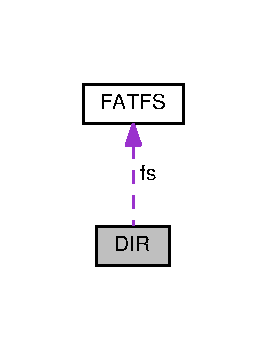
\includegraphics[width=128pt]{structDIR__coll__graph}
\end{center}
\end{figure}
\subsection*{Data Fields}
\begin{DoxyCompactItemize}
\item 
\hyperlink{structFATFS}{F\-A\-T\-F\-S} $\ast$ \hyperlink{structDIR_a312eaa66cb703fb2993ea98173dc0c9a}{fs}
\item 
\hyperlink{integer_8h_a197942eefa7db30960ae396d68339b97}{W\-O\-R\-D} \hyperlink{structDIR_aca2c95a99a04173917ec70c030891383}{id}
\item 
\hyperlink{integer_8h_a197942eefa7db30960ae396d68339b97}{W\-O\-R\-D} \hyperlink{structDIR_ab95119fbacbe45e3e9ee0f962b844092}{index}
\item 
\hyperlink{integer_8h_ad342ac907eb044443153a22f964bf0af}{D\-W\-O\-R\-D} \hyperlink{structDIR_a9212af5877b94d790dd3bab3aa320994}{sclust}
\item 
\hyperlink{integer_8h_ad342ac907eb044443153a22f964bf0af}{D\-W\-O\-R\-D} \hyperlink{structDIR_acfbb8ba2d6e73b6f999ceffd1857c190}{clust}
\item 
\hyperlink{integer_8h_ad342ac907eb044443153a22f964bf0af}{D\-W\-O\-R\-D} \hyperlink{structDIR_ad01fcc812ed0dad11a593574336adc9e}{sect}
\item 
\hyperlink{integer_8h_a4ae1dab0fb4b072a66584546209e7d58}{B\-Y\-T\-E} $\ast$ \hyperlink{structDIR_a6c2a8c0cf2d55ae99775e93a16593449}{dir}
\item 
\hyperlink{integer_8h_a4ae1dab0fb4b072a66584546209e7d58}{B\-Y\-T\-E} $\ast$ \hyperlink{structDIR_a32da2f31d6c3b6c42eef981cb0cfd2ee}{fn}
\end{DoxyCompactItemize}


\subsection{Field Documentation}
\hypertarget{structDIR_acfbb8ba2d6e73b6f999ceffd1857c190}{\index{D\-I\-R@{D\-I\-R}!clust@{clust}}
\index{clust@{clust}!DIR@{D\-I\-R}}
\subsubsection[{clust}]{\setlength{\rightskip}{0pt plus 5cm}{\bf D\-W\-O\-R\-D} D\-I\-R\-::clust}}\label{structDIR_acfbb8ba2d6e73b6f999ceffd1857c190}


Referenced by dir\-\_\-next(), and dir\-\_\-sdi().

\hypertarget{structDIR_a6c2a8c0cf2d55ae99775e93a16593449}{\index{D\-I\-R@{D\-I\-R}!dir@{dir}}
\index{dir@{dir}!DIR@{D\-I\-R}}
\subsubsection[{dir}]{\setlength{\rightskip}{0pt plus 5cm}{\bf B\-Y\-T\-E}$\ast$ D\-I\-R\-::dir}}\label{structDIR_a6c2a8c0cf2d55ae99775e93a16593449}


Referenced by dir\-\_\-alloc(), dir\-\_\-find(), dir\-\_\-next(), dir\-\_\-read(), dir\-\_\-register(), dir\-\_\-sdi(), f\-\_\-getlabel(), f\-\_\-open(), f\-\_\-setlabel(), and follow\-\_\-path().

\hypertarget{structDIR_a32da2f31d6c3b6c42eef981cb0cfd2ee}{\index{D\-I\-R@{D\-I\-R}!fn@{fn}}
\index{fn@{fn}!DIR@{D\-I\-R}}
\subsubsection[{fn}]{\setlength{\rightskip}{0pt plus 5cm}{\bf B\-Y\-T\-E}$\ast$ D\-I\-R\-::fn}}\label{structDIR_a32da2f31d6c3b6c42eef981cb0cfd2ee}


Referenced by create\-\_\-name(), dir\-\_\-find(), dir\-\_\-register(), and follow\-\_\-path().

\hypertarget{structDIR_a312eaa66cb703fb2993ea98173dc0c9a}{\index{D\-I\-R@{D\-I\-R}!fs@{fs}}
\index{fs@{fs}!DIR@{D\-I\-R}}
\subsubsection[{fs}]{\setlength{\rightskip}{0pt plus 5cm}{\bf F\-A\-T\-F\-S}$\ast$ D\-I\-R\-::fs}}\label{structDIR_a312eaa66cb703fb2993ea98173dc0c9a}


Referenced by dir\-\_\-alloc(), dir\-\_\-find(), dir\-\_\-next(), dir\-\_\-read(), dir\-\_\-register(), dir\-\_\-sdi(), f\-\_\-getlabel(), f\-\_\-open(), f\-\_\-setlabel(), and follow\-\_\-path().

\hypertarget{structDIR_aca2c95a99a04173917ec70c030891383}{\index{D\-I\-R@{D\-I\-R}!id@{id}}
\index{id@{id}!DIR@{D\-I\-R}}
\subsubsection[{id}]{\setlength{\rightskip}{0pt plus 5cm}{\bf W\-O\-R\-D} D\-I\-R\-::id}}\label{structDIR_aca2c95a99a04173917ec70c030891383}
\hypertarget{structDIR_ab95119fbacbe45e3e9ee0f962b844092}{\index{D\-I\-R@{D\-I\-R}!index@{index}}
\index{index@{index}!DIR@{D\-I\-R}}
\subsubsection[{index}]{\setlength{\rightskip}{0pt plus 5cm}{\bf W\-O\-R\-D} D\-I\-R\-::index}}\label{structDIR_ab95119fbacbe45e3e9ee0f962b844092}


Referenced by dir\-\_\-find(), dir\-\_\-next(), dir\-\_\-read(), dir\-\_\-register(), and dir\-\_\-sdi().

\hypertarget{structDIR_a9212af5877b94d790dd3bab3aa320994}{\index{D\-I\-R@{D\-I\-R}!sclust@{sclust}}
\index{sclust@{sclust}!DIR@{D\-I\-R}}
\subsubsection[{sclust}]{\setlength{\rightskip}{0pt plus 5cm}{\bf D\-W\-O\-R\-D} D\-I\-R\-::sclust}}\label{structDIR_a9212af5877b94d790dd3bab3aa320994}


Referenced by dir\-\_\-sdi(), f\-\_\-getlabel(), f\-\_\-setlabel(), and follow\-\_\-path().

\hypertarget{structDIR_ad01fcc812ed0dad11a593574336adc9e}{\index{D\-I\-R@{D\-I\-R}!sect@{sect}}
\index{sect@{sect}!DIR@{D\-I\-R}}
\subsubsection[{sect}]{\setlength{\rightskip}{0pt plus 5cm}{\bf D\-W\-O\-R\-D} D\-I\-R\-::sect}}\label{structDIR_ad01fcc812ed0dad11a593574336adc9e}


Referenced by dir\-\_\-alloc(), dir\-\_\-find(), dir\-\_\-next(), dir\-\_\-read(), dir\-\_\-register(), and dir\-\_\-sdi().



The documentation for this struct was generated from the following file\-:\begin{DoxyCompactItemize}
\item 
sd\-\_\-card/\hyperlink{ff_8h}{ff.\-h}\end{DoxyCompactItemize}

\hypertarget{structFATFS}{\section{F\-A\-T\-F\-S Struct Reference}
\label{structFATFS}\index{F\-A\-T\-F\-S@{F\-A\-T\-F\-S}}
}


{\ttfamily \#include $<$ff.\-h$>$}

\subsection*{Data Fields}
\begin{DoxyCompactItemize}
\item 
\hyperlink{integer_8h_a4ae1dab0fb4b072a66584546209e7d58}{B\-Y\-T\-E} \hyperlink{structFATFS_add27d97babe807b573eac98a71dc4ae5}{fs\-\_\-type}
\item 
\hyperlink{integer_8h_a4ae1dab0fb4b072a66584546209e7d58}{B\-Y\-T\-E} \hyperlink{structFATFS_a6a791560e2687e8b1569bfce61208d2d}{drv}
\item 
\hyperlink{integer_8h_a4ae1dab0fb4b072a66584546209e7d58}{B\-Y\-T\-E} \hyperlink{structFATFS_a504a1175f6dcc9a854b9da94463bd108}{csize}
\item 
\hyperlink{integer_8h_a4ae1dab0fb4b072a66584546209e7d58}{B\-Y\-T\-E} \hyperlink{structFATFS_a56716c7e7ac10cf46e73ffb2a2e9b545}{n\-\_\-fats}
\item 
\hyperlink{integer_8h_a4ae1dab0fb4b072a66584546209e7d58}{B\-Y\-T\-E} \hyperlink{structFATFS_a647e43c9ccae94b7274793d1909897de}{wflag}
\item 
\hyperlink{integer_8h_a4ae1dab0fb4b072a66584546209e7d58}{B\-Y\-T\-E} \hyperlink{structFATFS_a84e9cdc5a6a8e33ea7ec192058abf161}{fsi\-\_\-flag}
\item 
\hyperlink{integer_8h_a197942eefa7db30960ae396d68339b97}{W\-O\-R\-D} \hyperlink{structFATFS_a417095d7c20d56d417dc0998e0dd5a5c}{id}
\item 
\hyperlink{integer_8h_a197942eefa7db30960ae396d68339b97}{W\-O\-R\-D} \hyperlink{structFATFS_a189a00aa038044ffad0fc7f7dcf2aae1}{n\-\_\-rootdir}
\item 
\hyperlink{integer_8h_ad342ac907eb044443153a22f964bf0af}{D\-W\-O\-R\-D} \hyperlink{structFATFS_ad315def289218e26ab78ff90fde700d1}{last\-\_\-clust}
\item 
\hyperlink{integer_8h_ad342ac907eb044443153a22f964bf0af}{D\-W\-O\-R\-D} \hyperlink{structFATFS_a5fb49e6ac511bd97eaffdd636d0e4165}{free\-\_\-clust}
\item 
\hyperlink{integer_8h_ad342ac907eb044443153a22f964bf0af}{D\-W\-O\-R\-D} \hyperlink{structFATFS_a4900e785d26dfed6e456ceeb59ec29a7}{fsi\-\_\-sector}
\item 
\hyperlink{integer_8h_ad342ac907eb044443153a22f964bf0af}{D\-W\-O\-R\-D} \hyperlink{structFATFS_a8da50eeba6469bc20d60ca0cf9a1307c}{n\-\_\-fatent}
\item 
\hyperlink{integer_8h_ad342ac907eb044443153a22f964bf0af}{D\-W\-O\-R\-D} \hyperlink{structFATFS_a53e9560659f14e66f306c2c444198bf3}{fsize}
\item 
\hyperlink{integer_8h_ad342ac907eb044443153a22f964bf0af}{D\-W\-O\-R\-D} \hyperlink{structFATFS_a8f0ca578755749d204f59dc83f1a7649}{volbase}
\item 
\hyperlink{integer_8h_ad342ac907eb044443153a22f964bf0af}{D\-W\-O\-R\-D} \hyperlink{structFATFS_a848fba02c4aabe02ef2984e578f33d64}{fatbase}
\item 
\hyperlink{integer_8h_ad342ac907eb044443153a22f964bf0af}{D\-W\-O\-R\-D} \hyperlink{structFATFS_a3f72fd998dbcce4652a85a81fe944bc4}{dirbase}
\item 
\hyperlink{integer_8h_ad342ac907eb044443153a22f964bf0af}{D\-W\-O\-R\-D} \hyperlink{structFATFS_a5b6c0bc2e9fd2ae8ef714210a74a2d5d}{database}
\item 
\hyperlink{integer_8h_ad342ac907eb044443153a22f964bf0af}{D\-W\-O\-R\-D} \hyperlink{structFATFS_ac60e69c00e6bf7c25febfbac4dc1476b}{winsect}
\item 
\hyperlink{integer_8h_a4ae1dab0fb4b072a66584546209e7d58}{B\-Y\-T\-E} \hyperlink{structFATFS_a7cc35a593465e727ab87723c14610644}{win} \mbox{[}\hyperlink{ffconf_8h_ac271b697378912f17132cb9c7d0de024}{\-\_\-\-M\-A\-X\-\_\-\-S\-S}\mbox{]}
\end{DoxyCompactItemize}


\subsection{Field Documentation}
\hypertarget{structFATFS_a504a1175f6dcc9a854b9da94463bd108}{\index{F\-A\-T\-F\-S@{F\-A\-T\-F\-S}!csize@{csize}}
\index{csize@{csize}!FATFS@{F\-A\-T\-F\-S}}
\subsubsection[{csize}]{\setlength{\rightskip}{0pt plus 5cm}{\bf B\-Y\-T\-E} F\-A\-T\-F\-S\-::csize}}\label{structFATFS_a504a1175f6dcc9a854b9da94463bd108}


Referenced by chk\-\_\-mounted(), clust2sect(), dir\-\_\-next(), dir\-\_\-sdi(), f\-\_\-lseek(), f\-\_\-read(), f\-\_\-write(), and remove\-\_\-chain().

\hypertarget{structFATFS_a5b6c0bc2e9fd2ae8ef714210a74a2d5d}{\index{F\-A\-T\-F\-S@{F\-A\-T\-F\-S}!database@{database}}
\index{database@{database}!FATFS@{F\-A\-T\-F\-S}}
\subsubsection[{database}]{\setlength{\rightskip}{0pt plus 5cm}{\bf D\-W\-O\-R\-D} F\-A\-T\-F\-S\-::database}}\label{structFATFS_a5b6c0bc2e9fd2ae8ef714210a74a2d5d}


Referenced by chk\-\_\-mounted(), and clust2sect().

\hypertarget{structFATFS_a3f72fd998dbcce4652a85a81fe944bc4}{\index{F\-A\-T\-F\-S@{F\-A\-T\-F\-S}!dirbase@{dirbase}}
\index{dirbase@{dirbase}!FATFS@{F\-A\-T\-F\-S}}
\subsubsection[{dirbase}]{\setlength{\rightskip}{0pt plus 5cm}{\bf D\-W\-O\-R\-D} F\-A\-T\-F\-S\-::dirbase}}\label{structFATFS_a3f72fd998dbcce4652a85a81fe944bc4}


Referenced by chk\-\_\-mounted(), and dir\-\_\-sdi().

\hypertarget{structFATFS_a6a791560e2687e8b1569bfce61208d2d}{\index{F\-A\-T\-F\-S@{F\-A\-T\-F\-S}!drv@{drv}}
\index{drv@{drv}!FATFS@{F\-A\-T\-F\-S}}
\subsubsection[{drv}]{\setlength{\rightskip}{0pt plus 5cm}{\bf B\-Y\-T\-E} F\-A\-T\-F\-S\-::drv}}\label{structFATFS_a6a791560e2687e8b1569bfce61208d2d}


Referenced by check\-\_\-fs(), chk\-\_\-mounted(), f\-\_\-lseek(), f\-\_\-read(), f\-\_\-sync(), f\-\_\-write(), move\-\_\-window(), remove\-\_\-chain(), sync\-\_\-fs(), sync\-\_\-window(), and validate().

\hypertarget{structFATFS_a848fba02c4aabe02ef2984e578f33d64}{\index{F\-A\-T\-F\-S@{F\-A\-T\-F\-S}!fatbase@{fatbase}}
\index{fatbase@{fatbase}!FATFS@{F\-A\-T\-F\-S}}
\subsubsection[{fatbase}]{\setlength{\rightskip}{0pt plus 5cm}{\bf D\-W\-O\-R\-D} F\-A\-T\-F\-S\-::fatbase}}\label{structFATFS_a848fba02c4aabe02ef2984e578f33d64}


Referenced by chk\-\_\-mounted(), get\-\_\-fat(), put\-\_\-fat(), and sync\-\_\-window().

\hypertarget{structFATFS_a5fb49e6ac511bd97eaffdd636d0e4165}{\index{F\-A\-T\-F\-S@{F\-A\-T\-F\-S}!free\-\_\-clust@{free\-\_\-clust}}
\index{free\-\_\-clust@{free\-\_\-clust}!FATFS@{F\-A\-T\-F\-S}}
\subsubsection[{free\-\_\-clust}]{\setlength{\rightskip}{0pt plus 5cm}{\bf D\-W\-O\-R\-D} F\-A\-T\-F\-S\-::free\-\_\-clust}}\label{structFATFS_a5fb49e6ac511bd97eaffdd636d0e4165}


Referenced by chk\-\_\-mounted(), create\-\_\-chain(), remove\-\_\-chain(), and sync\-\_\-fs().

\hypertarget{structFATFS_add27d97babe807b573eac98a71dc4ae5}{\index{F\-A\-T\-F\-S@{F\-A\-T\-F\-S}!fs\-\_\-type@{fs\-\_\-type}}
\index{fs\-\_\-type@{fs\-\_\-type}!FATFS@{F\-A\-T\-F\-S}}
\subsubsection[{fs\-\_\-type}]{\setlength{\rightskip}{0pt plus 5cm}{\bf B\-Y\-T\-E} F\-A\-T\-F\-S\-::fs\-\_\-type}}\label{structFATFS_add27d97babe807b573eac98a71dc4ae5}


Referenced by chk\-\_\-mounted(), dir\-\_\-sdi(), f\-\_\-getlabel(), f\-\_\-mount(), get\-\_\-fat(), ld\-\_\-clust(), put\-\_\-fat(), sync\-\_\-fs(), and validate().

\hypertarget{structFATFS_a84e9cdc5a6a8e33ea7ec192058abf161}{\index{F\-A\-T\-F\-S@{F\-A\-T\-F\-S}!fsi\-\_\-flag@{fsi\-\_\-flag}}
\index{fsi\-\_\-flag@{fsi\-\_\-flag}!FATFS@{F\-A\-T\-F\-S}}
\subsubsection[{fsi\-\_\-flag}]{\setlength{\rightskip}{0pt plus 5cm}{\bf B\-Y\-T\-E} F\-A\-T\-F\-S\-::fsi\-\_\-flag}}\label{structFATFS_a84e9cdc5a6a8e33ea7ec192058abf161}


Referenced by chk\-\_\-mounted(), create\-\_\-chain(), remove\-\_\-chain(), and sync\-\_\-fs().

\hypertarget{structFATFS_a4900e785d26dfed6e456ceeb59ec29a7}{\index{F\-A\-T\-F\-S@{F\-A\-T\-F\-S}!fsi\-\_\-sector@{fsi\-\_\-sector}}
\index{fsi\-\_\-sector@{fsi\-\_\-sector}!FATFS@{F\-A\-T\-F\-S}}
\subsubsection[{fsi\-\_\-sector}]{\setlength{\rightskip}{0pt plus 5cm}{\bf D\-W\-O\-R\-D} F\-A\-T\-F\-S\-::fsi\-\_\-sector}}\label{structFATFS_a4900e785d26dfed6e456ceeb59ec29a7}


Referenced by chk\-\_\-mounted(), and sync\-\_\-fs().

\hypertarget{structFATFS_a53e9560659f14e66f306c2c444198bf3}{\index{F\-A\-T\-F\-S@{F\-A\-T\-F\-S}!fsize@{fsize}}
\index{fsize@{fsize}!FATFS@{F\-A\-T\-F\-S}}
\subsubsection[{fsize}]{\setlength{\rightskip}{0pt plus 5cm}{\bf D\-W\-O\-R\-D} F\-A\-T\-F\-S\-::fsize}}\label{structFATFS_a53e9560659f14e66f306c2c444198bf3}


Referenced by chk\-\_\-mounted(), and sync\-\_\-window().

\hypertarget{structFATFS_a417095d7c20d56d417dc0998e0dd5a5c}{\index{F\-A\-T\-F\-S@{F\-A\-T\-F\-S}!id@{id}}
\index{id@{id}!FATFS@{F\-A\-T\-F\-S}}
\subsubsection[{id}]{\setlength{\rightskip}{0pt plus 5cm}{\bf W\-O\-R\-D} F\-A\-T\-F\-S\-::id}}\label{structFATFS_a417095d7c20d56d417dc0998e0dd5a5c}


Referenced by chk\-\_\-mounted(), f\-\_\-open(), and validate().

\hypertarget{structFATFS_ad315def289218e26ab78ff90fde700d1}{\index{F\-A\-T\-F\-S@{F\-A\-T\-F\-S}!last\-\_\-clust@{last\-\_\-clust}}
\index{last\-\_\-clust@{last\-\_\-clust}!FATFS@{F\-A\-T\-F\-S}}
\subsubsection[{last\-\_\-clust}]{\setlength{\rightskip}{0pt plus 5cm}{\bf D\-W\-O\-R\-D} F\-A\-T\-F\-S\-::last\-\_\-clust}}\label{structFATFS_ad315def289218e26ab78ff90fde700d1}


Referenced by chk\-\_\-mounted(), create\-\_\-chain(), f\-\_\-open(), and sync\-\_\-fs().

\hypertarget{structFATFS_a8da50eeba6469bc20d60ca0cf9a1307c}{\index{F\-A\-T\-F\-S@{F\-A\-T\-F\-S}!n\-\_\-fatent@{n\-\_\-fatent}}
\index{n\-\_\-fatent@{n\-\_\-fatent}!FATFS@{F\-A\-T\-F\-S}}
\subsubsection[{n\-\_\-fatent}]{\setlength{\rightskip}{0pt plus 5cm}{\bf D\-W\-O\-R\-D} F\-A\-T\-F\-S\-::n\-\_\-fatent}}\label{structFATFS_a8da50eeba6469bc20d60ca0cf9a1307c}


Referenced by chk\-\_\-mounted(), clust2sect(), create\-\_\-chain(), dir\-\_\-next(), dir\-\_\-sdi(), f\-\_\-lseek(), get\-\_\-fat(), put\-\_\-fat(), and remove\-\_\-chain().

\hypertarget{structFATFS_a56716c7e7ac10cf46e73ffb2a2e9b545}{\index{F\-A\-T\-F\-S@{F\-A\-T\-F\-S}!n\-\_\-fats@{n\-\_\-fats}}
\index{n\-\_\-fats@{n\-\_\-fats}!FATFS@{F\-A\-T\-F\-S}}
\subsubsection[{n\-\_\-fats}]{\setlength{\rightskip}{0pt plus 5cm}{\bf B\-Y\-T\-E} F\-A\-T\-F\-S\-::n\-\_\-fats}}\label{structFATFS_a56716c7e7ac10cf46e73ffb2a2e9b545}


Referenced by chk\-\_\-mounted(), and sync\-\_\-window().

\hypertarget{structFATFS_a189a00aa038044ffad0fc7f7dcf2aae1}{\index{F\-A\-T\-F\-S@{F\-A\-T\-F\-S}!n\-\_\-rootdir@{n\-\_\-rootdir}}
\index{n\-\_\-rootdir@{n\-\_\-rootdir}!FATFS@{F\-A\-T\-F\-S}}
\subsubsection[{n\-\_\-rootdir}]{\setlength{\rightskip}{0pt plus 5cm}{\bf W\-O\-R\-D} F\-A\-T\-F\-S\-::n\-\_\-rootdir}}\label{structFATFS_a189a00aa038044ffad0fc7f7dcf2aae1}


Referenced by chk\-\_\-mounted(), dir\-\_\-next(), and dir\-\_\-sdi().

\hypertarget{structFATFS_a8f0ca578755749d204f59dc83f1a7649}{\index{F\-A\-T\-F\-S@{F\-A\-T\-F\-S}!volbase@{volbase}}
\index{volbase@{volbase}!FATFS@{F\-A\-T\-F\-S}}
\subsubsection[{volbase}]{\setlength{\rightskip}{0pt plus 5cm}{\bf D\-W\-O\-R\-D} F\-A\-T\-F\-S\-::volbase}}\label{structFATFS_a8f0ca578755749d204f59dc83f1a7649}


Referenced by chk\-\_\-mounted(), and f\-\_\-getlabel().

\hypertarget{structFATFS_a647e43c9ccae94b7274793d1909897de}{\index{F\-A\-T\-F\-S@{F\-A\-T\-F\-S}!wflag@{wflag}}
\index{wflag@{wflag}!FATFS@{F\-A\-T\-F\-S}}
\subsubsection[{wflag}]{\setlength{\rightskip}{0pt plus 5cm}{\bf B\-Y\-T\-E} F\-A\-T\-F\-S\-::wflag}}\label{structFATFS_a647e43c9ccae94b7274793d1909897de}


Referenced by chk\-\_\-mounted(), dir\-\_\-next(), dir\-\_\-register(), f\-\_\-open(), f\-\_\-read(), f\-\_\-setlabel(), f\-\_\-sync(), f\-\_\-write(), put\-\_\-fat(), and sync\-\_\-window().

\hypertarget{structFATFS_a7cc35a593465e727ab87723c14610644}{\index{F\-A\-T\-F\-S@{F\-A\-T\-F\-S}!win@{win}}
\index{win@{win}!FATFS@{F\-A\-T\-F\-S}}
\subsubsection[{win}]{\setlength{\rightskip}{0pt plus 5cm}{\bf B\-Y\-T\-E} F\-A\-T\-F\-S\-::win\mbox{[}{\bf \-\_\-\-M\-A\-X\-\_\-\-S\-S}\mbox{]}}}\label{structFATFS_a7cc35a593465e727ab87723c14610644}


Referenced by check\-\_\-fs(), chk\-\_\-mounted(), dir\-\_\-next(), dir\-\_\-sdi(), f\-\_\-getlabel(), f\-\_\-read(), f\-\_\-write(), get\-\_\-fat(), move\-\_\-window(), put\-\_\-fat(), sync\-\_\-fs(), and sync\-\_\-window().

\hypertarget{structFATFS_ac60e69c00e6bf7c25febfbac4dc1476b}{\index{F\-A\-T\-F\-S@{F\-A\-T\-F\-S}!winsect@{winsect}}
\index{winsect@{winsect}!FATFS@{F\-A\-T\-F\-S}}
\subsubsection[{winsect}]{\setlength{\rightskip}{0pt plus 5cm}{\bf D\-W\-O\-R\-D} F\-A\-T\-F\-S\-::winsect}}\label{structFATFS_ac60e69c00e6bf7c25febfbac4dc1476b}


Referenced by chk\-\_\-mounted(), dir\-\_\-next(), f\-\_\-open(), f\-\_\-read(), f\-\_\-write(), move\-\_\-window(), sync\-\_\-fs(), and sync\-\_\-window().



The documentation for this struct was generated from the following file\-:\begin{DoxyCompactItemize}
\item 
sd\-\_\-card/\hyperlink{ff_8h}{ff.\-h}\end{DoxyCompactItemize}

\hypertarget{structFIL}{\section{F\-I\-L Struct Reference}
\label{structFIL}\index{F\-I\-L@{F\-I\-L}}
}


{\ttfamily \#include $<$ff.\-h$>$}



Collaboration diagram for F\-I\-L\-:\nopagebreak
\begin{figure}[H]
\begin{center}
\leavevmode
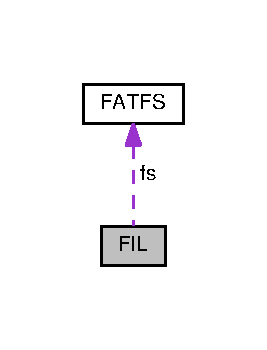
\includegraphics[width=128pt]{structFIL__coll__graph}
\end{center}
\end{figure}
\subsection*{Data Fields}
\begin{DoxyCompactItemize}
\item 
\hyperlink{structFATFS}{F\-A\-T\-F\-S} $\ast$ \hyperlink{structFIL_a42376a6797a06228911c8b836c1e9030}{fs}
\item 
\hyperlink{integer_8h_a197942eefa7db30960ae396d68339b97}{W\-O\-R\-D} \hyperlink{structFIL_af7cae0063b0045fb7078b560101ba8f2}{id}
\item 
\hyperlink{integer_8h_a4ae1dab0fb4b072a66584546209e7d58}{B\-Y\-T\-E} \hyperlink{structFIL_ac409508881f5a16f2998ae675072b376}{flag}
\item 
\hyperlink{integer_8h_a4ae1dab0fb4b072a66584546209e7d58}{B\-Y\-T\-E} \hyperlink{structFIL_a17f891ef69059bd879f6492473cfceae}{pad1}
\item 
\hyperlink{integer_8h_ad342ac907eb044443153a22f964bf0af}{D\-W\-O\-R\-D} \hyperlink{structFIL_a75d29cf9257c827d117887b9f924c4a9}{fptr}
\item 
\hyperlink{integer_8h_ad342ac907eb044443153a22f964bf0af}{D\-W\-O\-R\-D} \hyperlink{structFIL_aa00790d40d7b0081c345fd4f76e22b70}{fsize}
\item 
\hyperlink{integer_8h_ad342ac907eb044443153a22f964bf0af}{D\-W\-O\-R\-D} \hyperlink{structFIL_ad308b74c8d6975c6a9c30d90b4124c40}{sclust}
\item 
\hyperlink{integer_8h_ad342ac907eb044443153a22f964bf0af}{D\-W\-O\-R\-D} \hyperlink{structFIL_aa41312aba551b9a6d1c9d3c8c7d2734b}{clust}
\item 
\hyperlink{integer_8h_ad342ac907eb044443153a22f964bf0af}{D\-W\-O\-R\-D} \hyperlink{structFIL_ab3d4165d6fd32ac71a130d835fbf0b4d}{dsect}
\item 
\hyperlink{integer_8h_ad342ac907eb044443153a22f964bf0af}{D\-W\-O\-R\-D} \hyperlink{structFIL_ab203794f939ad4480e81dfa488770783}{dir\-\_\-sect}
\item 
\hyperlink{integer_8h_a4ae1dab0fb4b072a66584546209e7d58}{B\-Y\-T\-E} $\ast$ \hyperlink{structFIL_a5af9e9fb312b629220eaf684dd28c4a9}{dir\-\_\-ptr}
\end{DoxyCompactItemize}


\subsection{Field Documentation}
\hypertarget{structFIL_aa41312aba551b9a6d1c9d3c8c7d2734b}{\index{F\-I\-L@{F\-I\-L}!clust@{clust}}
\index{clust@{clust}!FIL@{F\-I\-L}}
\subsubsection[{clust}]{\setlength{\rightskip}{0pt plus 5cm}{\bf D\-W\-O\-R\-D} F\-I\-L\-::clust}}\label{structFIL_aa41312aba551b9a6d1c9d3c8c7d2734b}


Referenced by f\-\_\-lseek(), f\-\_\-read(), and f\-\_\-write().

\hypertarget{structFIL_a5af9e9fb312b629220eaf684dd28c4a9}{\index{F\-I\-L@{F\-I\-L}!dir\-\_\-ptr@{dir\-\_\-ptr}}
\index{dir\-\_\-ptr@{dir\-\_\-ptr}!FIL@{F\-I\-L}}
\subsubsection[{dir\-\_\-ptr}]{\setlength{\rightskip}{0pt plus 5cm}{\bf B\-Y\-T\-E}$\ast$ F\-I\-L\-::dir\-\_\-ptr}}\label{structFIL_a5af9e9fb312b629220eaf684dd28c4a9}


Referenced by f\-\_\-open(), and f\-\_\-sync().

\hypertarget{structFIL_ab203794f939ad4480e81dfa488770783}{\index{F\-I\-L@{F\-I\-L}!dir\-\_\-sect@{dir\-\_\-sect}}
\index{dir\-\_\-sect@{dir\-\_\-sect}!FIL@{F\-I\-L}}
\subsubsection[{dir\-\_\-sect}]{\setlength{\rightskip}{0pt plus 5cm}{\bf D\-W\-O\-R\-D} F\-I\-L\-::dir\-\_\-sect}}\label{structFIL_ab203794f939ad4480e81dfa488770783}


Referenced by f\-\_\-open(), and f\-\_\-sync().

\hypertarget{structFIL_ab3d4165d6fd32ac71a130d835fbf0b4d}{\index{F\-I\-L@{F\-I\-L}!dsect@{dsect}}
\index{dsect@{dsect}!FIL@{F\-I\-L}}
\subsubsection[{dsect}]{\setlength{\rightskip}{0pt plus 5cm}{\bf D\-W\-O\-R\-D} F\-I\-L\-::dsect}}\label{structFIL_ab3d4165d6fd32ac71a130d835fbf0b4d}


Referenced by f\-\_\-lseek(), f\-\_\-open(), f\-\_\-read(), f\-\_\-sync(), and f\-\_\-write().

\hypertarget{structFIL_ac409508881f5a16f2998ae675072b376}{\index{F\-I\-L@{F\-I\-L}!flag@{flag}}
\index{flag@{flag}!FIL@{F\-I\-L}}
\subsubsection[{flag}]{\setlength{\rightskip}{0pt plus 5cm}{\bf B\-Y\-T\-E} F\-I\-L\-::flag}}\label{structFIL_ac409508881f5a16f2998ae675072b376}


Referenced by f\-\_\-lseek(), f\-\_\-open(), f\-\_\-read(), f\-\_\-sync(), and f\-\_\-write().

\hypertarget{structFIL_a75d29cf9257c827d117887b9f924c4a9}{\index{F\-I\-L@{F\-I\-L}!fptr@{fptr}}
\index{fptr@{fptr}!FIL@{F\-I\-L}}
\subsubsection[{fptr}]{\setlength{\rightskip}{0pt plus 5cm}{\bf D\-W\-O\-R\-D} F\-I\-L\-::fptr}}\label{structFIL_a75d29cf9257c827d117887b9f924c4a9}


Referenced by f\-\_\-lseek(), f\-\_\-open(), f\-\_\-read(), and f\-\_\-write().

\hypertarget{structFIL_a42376a6797a06228911c8b836c1e9030}{\index{F\-I\-L@{F\-I\-L}!fs@{fs}}
\index{fs@{fs}!FIL@{F\-I\-L}}
\subsubsection[{fs}]{\setlength{\rightskip}{0pt plus 5cm}{\bf F\-A\-T\-F\-S}$\ast$ F\-I\-L\-::fs}}\label{structFIL_a42376a6797a06228911c8b836c1e9030}


Referenced by f\-\_\-close(), f\-\_\-lseek(), f\-\_\-open(), f\-\_\-read(), f\-\_\-sync(), f\-\_\-write(), and validate().

\hypertarget{structFIL_aa00790d40d7b0081c345fd4f76e22b70}{\index{F\-I\-L@{F\-I\-L}!fsize@{fsize}}
\index{fsize@{fsize}!FIL@{F\-I\-L}}
\subsubsection[{fsize}]{\setlength{\rightskip}{0pt plus 5cm}{\bf D\-W\-O\-R\-D} F\-I\-L\-::fsize}}\label{structFIL_aa00790d40d7b0081c345fd4f76e22b70}


Referenced by f\-\_\-lseek(), f\-\_\-open(), f\-\_\-read(), f\-\_\-sync(), and f\-\_\-write().

\hypertarget{structFIL_af7cae0063b0045fb7078b560101ba8f2}{\index{F\-I\-L@{F\-I\-L}!id@{id}}
\index{id@{id}!FIL@{F\-I\-L}}
\subsubsection[{id}]{\setlength{\rightskip}{0pt plus 5cm}{\bf W\-O\-R\-D} F\-I\-L\-::id}}\label{structFIL_af7cae0063b0045fb7078b560101ba8f2}


Referenced by f\-\_\-open(), and validate().

\hypertarget{structFIL_a17f891ef69059bd879f6492473cfceae}{\index{F\-I\-L@{F\-I\-L}!pad1@{pad1}}
\index{pad1@{pad1}!FIL@{F\-I\-L}}
\subsubsection[{pad1}]{\setlength{\rightskip}{0pt plus 5cm}{\bf B\-Y\-T\-E} F\-I\-L\-::pad1}}\label{structFIL_a17f891ef69059bd879f6492473cfceae}
\hypertarget{structFIL_ad308b74c8d6975c6a9c30d90b4124c40}{\index{F\-I\-L@{F\-I\-L}!sclust@{sclust}}
\index{sclust@{sclust}!FIL@{F\-I\-L}}
\subsubsection[{sclust}]{\setlength{\rightskip}{0pt plus 5cm}{\bf D\-W\-O\-R\-D} F\-I\-L\-::sclust}}\label{structFIL_ad308b74c8d6975c6a9c30d90b4124c40}


Referenced by f\-\_\-lseek(), f\-\_\-open(), f\-\_\-read(), f\-\_\-sync(), and f\-\_\-write().



The documentation for this struct was generated from the following file\-:\begin{DoxyCompactItemize}
\item 
sd\-\_\-card/\hyperlink{ff_8h}{ff.\-h}\end{DoxyCompactItemize}

\hypertarget{structFILINFO}{\section{F\-I\-L\-I\-N\-F\-O Struct Reference}
\label{structFILINFO}\index{F\-I\-L\-I\-N\-F\-O@{F\-I\-L\-I\-N\-F\-O}}
}


{\ttfamily \#include $<$ff.\-h$>$}

\subsection*{Data Fields}
\begin{DoxyCompactItemize}
\item 
\hyperlink{integer_8h_ad342ac907eb044443153a22f964bf0af}{D\-W\-O\-R\-D} \hyperlink{structFILINFO_aee7441af7dc0c443d1e1e6011cc7dcac}{fsize}
\item 
\hyperlink{integer_8h_a197942eefa7db30960ae396d68339b97}{W\-O\-R\-D} \hyperlink{structFILINFO_a7c01c48a15b1b49da459924437b0bd52}{fdate}
\item 
\hyperlink{integer_8h_a197942eefa7db30960ae396d68339b97}{W\-O\-R\-D} \hyperlink{structFILINFO_ae0f751b79621bf7b29669f177bbe6b9a}{ftime}
\item 
\hyperlink{integer_8h_a4ae1dab0fb4b072a66584546209e7d58}{B\-Y\-T\-E} \hyperlink{structFILINFO_a838d542585831b085537b363f18205c0}{fattrib}
\item 
\hyperlink{ff_8h_a03bdb8ce5895c7e261aadc2529637546}{T\-C\-H\-A\-R} \hyperlink{structFILINFO_abd852510f2f79b4ec773156d8942dc7c}{fname} \mbox{[}13\mbox{]}
\end{DoxyCompactItemize}


\subsection{Field Documentation}
\hypertarget{structFILINFO_a838d542585831b085537b363f18205c0}{\index{F\-I\-L\-I\-N\-F\-O@{F\-I\-L\-I\-N\-F\-O}!fattrib@{fattrib}}
\index{fattrib@{fattrib}!FILINFO@{F\-I\-L\-I\-N\-F\-O}}
\subsubsection[{fattrib}]{\setlength{\rightskip}{0pt plus 5cm}{\bf B\-Y\-T\-E} F\-I\-L\-I\-N\-F\-O\-::fattrib}}\label{structFILINFO_a838d542585831b085537b363f18205c0}
\hypertarget{structFILINFO_a7c01c48a15b1b49da459924437b0bd52}{\index{F\-I\-L\-I\-N\-F\-O@{F\-I\-L\-I\-N\-F\-O}!fdate@{fdate}}
\index{fdate@{fdate}!FILINFO@{F\-I\-L\-I\-N\-F\-O}}
\subsubsection[{fdate}]{\setlength{\rightskip}{0pt plus 5cm}{\bf W\-O\-R\-D} F\-I\-L\-I\-N\-F\-O\-::fdate}}\label{structFILINFO_a7c01c48a15b1b49da459924437b0bd52}
\hypertarget{structFILINFO_abd852510f2f79b4ec773156d8942dc7c}{\index{F\-I\-L\-I\-N\-F\-O@{F\-I\-L\-I\-N\-F\-O}!fname@{fname}}
\index{fname@{fname}!FILINFO@{F\-I\-L\-I\-N\-F\-O}}
\subsubsection[{fname}]{\setlength{\rightskip}{0pt plus 5cm}{\bf T\-C\-H\-A\-R} F\-I\-L\-I\-N\-F\-O\-::fname\mbox{[}13\mbox{]}}}\label{structFILINFO_abd852510f2f79b4ec773156d8942dc7c}
\hypertarget{structFILINFO_aee7441af7dc0c443d1e1e6011cc7dcac}{\index{F\-I\-L\-I\-N\-F\-O@{F\-I\-L\-I\-N\-F\-O}!fsize@{fsize}}
\index{fsize@{fsize}!FILINFO@{F\-I\-L\-I\-N\-F\-O}}
\subsubsection[{fsize}]{\setlength{\rightskip}{0pt plus 5cm}{\bf D\-W\-O\-R\-D} F\-I\-L\-I\-N\-F\-O\-::fsize}}\label{structFILINFO_aee7441af7dc0c443d1e1e6011cc7dcac}
\hypertarget{structFILINFO_ae0f751b79621bf7b29669f177bbe6b9a}{\index{F\-I\-L\-I\-N\-F\-O@{F\-I\-L\-I\-N\-F\-O}!ftime@{ftime}}
\index{ftime@{ftime}!FILINFO@{F\-I\-L\-I\-N\-F\-O}}
\subsubsection[{ftime}]{\setlength{\rightskip}{0pt plus 5cm}{\bf W\-O\-R\-D} F\-I\-L\-I\-N\-F\-O\-::ftime}}\label{structFILINFO_ae0f751b79621bf7b29669f177bbe6b9a}


The documentation for this struct was generated from the following file\-:\begin{DoxyCompactItemize}
\item 
sd\-\_\-card/\hyperlink{ff_8h}{ff.\-h}\end{DoxyCompactItemize}

\hypertarget{structonode}{\section{onode Struct Reference}
\label{structonode}\index{onode@{onode}}
}


{\ttfamily \#include $<$list.\-h$>$}



Collaboration diagram for onode\-:\nopagebreak
\begin{figure}[H]
\begin{center}
\leavevmode
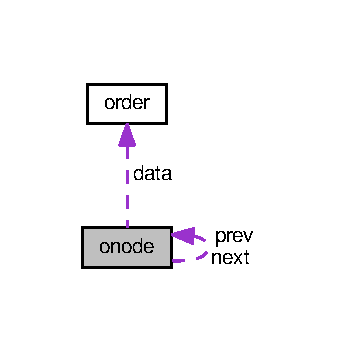
\includegraphics[width=162pt]{structonode__coll__graph}
\end{center}
\end{figure}
\subsection*{Data Fields}
\begin{DoxyCompactItemize}
\item 
struct \hyperlink{structorder}{order} $\ast$ \hyperlink{structonode_ab7312b747804b1474c83bd2bb7df8d3c}{data}
\item 
struct \hyperlink{structonode}{onode} $\ast$ \hyperlink{structonode_ac9704e6f9b12c04f52e61c856f8c1e29}{next}
\item 
struct \hyperlink{structonode}{onode} $\ast$ \hyperlink{structonode_a597f99367f877e2e4a9cafe4be30e837}{prev}
\end{DoxyCompactItemize}


\subsection{Field Documentation}
\hypertarget{structonode_ab7312b747804b1474c83bd2bb7df8d3c}{\index{onode@{onode}!data@{data}}
\index{data@{data}!onode@{onode}}
\subsubsection[{data}]{\setlength{\rightskip}{0pt plus 5cm}struct {\bf order}$\ast$ onode\-::data}}\label{structonode_ab7312b747804b1474c83bd2bb7df8d3c}


Referenced by delete\-List(), delete\-Node(), get\-Order\-Data(), get\-Order\-Node(), new\-Node\-By\-Ref(), print\-List(), sort(), and swap().

\hypertarget{structonode_ac9704e6f9b12c04f52e61c856f8c1e29}{\index{onode@{onode}!next@{next}}
\index{next@{next}!onode@{onode}}
\subsubsection[{next}]{\setlength{\rightskip}{0pt plus 5cm}struct {\bf onode}$\ast$ onode\-::next}}\label{structonode_ac9704e6f9b12c04f52e61c856f8c1e29}


Referenced by delete\-Just\-List(), delete\-List(), evict\-Node(), get\-Next\-Order(), get\-Order\-Node(), insert\-Node(), print\-List(), and push\-Node().

\hypertarget{structonode_a597f99367f877e2e4a9cafe4be30e837}{\index{onode@{onode}!prev@{prev}}
\index{prev@{prev}!onode@{onode}}
\subsubsection[{prev}]{\setlength{\rightskip}{0pt plus 5cm}struct {\bf onode}$\ast$ onode\-::prev}}\label{structonode_a597f99367f877e2e4a9cafe4be30e837}


Referenced by evict\-Node(), get\-Prev\-Order(), insert\-Node(), and push\-Node().



The documentation for this struct was generated from the following file\-:\begin{DoxyCompactItemize}
\item 
list/\hyperlink{list_8h}{list.\-h}\end{DoxyCompactItemize}

\hypertarget{structorder}{\section{order Struct Reference}
\label{structorder}\index{order@{order}}
}


{\ttfamily \#include $<$list.\-h$>$}

\subsection*{Data Fields}
\begin{DoxyCompactItemize}
\item 
int \hyperlink{structorder_a4328e44fed73692e76eb23049f1d972a}{id}
\item 
char \hyperlink{structorder_a8c533b3d1568db6bb3132be3a58b14ee}{bank1\-\_\-startstop}
\item 
char \hyperlink{structorder_a0a9f68e4094dfe71346d413df3c5f722}{bank1\-\_\-note}
\item 
char \hyperlink{structorder_aa07172101a0760b7b19335fe24f9e462}{bank2\-\_\-startstop}
\item 
char \hyperlink{structorder_adc801e65b34bd19e8db0decc145bc791}{bank2\-\_\-note}
\item 
char \hyperlink{structorder_a92057c9ceb6ae7cc28814e5a8b3ff3e2}{bank3\-\_\-startstop}
\item 
char \hyperlink{structorder_aed04b397690a0528443e701f41a99e8f}{bank3\-\_\-note}
\end{DoxyCompactItemize}


\subsection{Field Documentation}
\hypertarget{structorder_a0a9f68e4094dfe71346d413df3c5f722}{\index{order@{order}!bank1\-\_\-note@{bank1\-\_\-note}}
\index{bank1\-\_\-note@{bank1\-\_\-note}!order@{order}}
\subsubsection[{bank1\-\_\-note}]{\setlength{\rightskip}{0pt plus 5cm}char order\-::bank1\-\_\-note}}\label{structorder_a0a9f68e4094dfe71346d413df3c5f722}


Referenced by get\-Order\-Note(), main(), new\-Node(), and set\-Order\-Note().

\hypertarget{structorder_a8c533b3d1568db6bb3132be3a58b14ee}{\index{order@{order}!bank1\-\_\-startstop@{bank1\-\_\-startstop}}
\index{bank1\-\_\-startstop@{bank1\-\_\-startstop}!order@{order}}
\subsubsection[{bank1\-\_\-startstop}]{\setlength{\rightskip}{0pt plus 5cm}char order\-::bank1\-\_\-startstop}}\label{structorder_a8c533b3d1568db6bb3132be3a58b14ee}


Referenced by get\-Order\-Startstop(), main(), new\-Node(), and set\-Order\-Startstop().

\hypertarget{structorder_adc801e65b34bd19e8db0decc145bc791}{\index{order@{order}!bank2\-\_\-note@{bank2\-\_\-note}}
\index{bank2\-\_\-note@{bank2\-\_\-note}!order@{order}}
\subsubsection[{bank2\-\_\-note}]{\setlength{\rightskip}{0pt plus 5cm}char order\-::bank2\-\_\-note}}\label{structorder_adc801e65b34bd19e8db0decc145bc791}


Referenced by get\-Order\-Note(), main(), new\-Node(), and set\-Order\-Note().

\hypertarget{structorder_aa07172101a0760b7b19335fe24f9e462}{\index{order@{order}!bank2\-\_\-startstop@{bank2\-\_\-startstop}}
\index{bank2\-\_\-startstop@{bank2\-\_\-startstop}!order@{order}}
\subsubsection[{bank2\-\_\-startstop}]{\setlength{\rightskip}{0pt plus 5cm}char order\-::bank2\-\_\-startstop}}\label{structorder_aa07172101a0760b7b19335fe24f9e462}


Referenced by get\-Order\-Startstop(), main(), new\-Node(), and set\-Order\-Startstop().

\hypertarget{structorder_aed04b397690a0528443e701f41a99e8f}{\index{order@{order}!bank3\-\_\-note@{bank3\-\_\-note}}
\index{bank3\-\_\-note@{bank3\-\_\-note}!order@{order}}
\subsubsection[{bank3\-\_\-note}]{\setlength{\rightskip}{0pt plus 5cm}char order\-::bank3\-\_\-note}}\label{structorder_aed04b397690a0528443e701f41a99e8f}


Referenced by get\-Order\-Note(), main(), new\-Node(), and set\-Order\-Note().

\hypertarget{structorder_a92057c9ceb6ae7cc28814e5a8b3ff3e2}{\index{order@{order}!bank3\-\_\-startstop@{bank3\-\_\-startstop}}
\index{bank3\-\_\-startstop@{bank3\-\_\-startstop}!order@{order}}
\subsubsection[{bank3\-\_\-startstop}]{\setlength{\rightskip}{0pt plus 5cm}char order\-::bank3\-\_\-startstop}}\label{structorder_a92057c9ceb6ae7cc28814e5a8b3ff3e2}


Referenced by get\-Order\-Startstop(), main(), new\-Node(), and set\-Order\-Startstop().

\hypertarget{structorder_a4328e44fed73692e76eb23049f1d972a}{\index{order@{order}!id@{id}}
\index{id@{id}!order@{order}}
\subsubsection[{id}]{\setlength{\rightskip}{0pt plus 5cm}int order\-::id}}\label{structorder_a4328e44fed73692e76eb23049f1d972a}


Referenced by get\-Order\-Id(), get\-Order\-Node(), main(), new\-Node(), and set\-Order\-Id().



The documentation for this struct was generated from the following file\-:\begin{DoxyCompactItemize}
\item 
list/\hyperlink{list_8h}{list.\-h}\end{DoxyCompactItemize}

\chapter{File Documentation}
\hypertarget{config_8h}{\section{config.\-h File Reference}
\label{config_8h}\index{config.\-h@{config.\-h}}
}
This graph shows which files directly or indirectly include this file\-:\nopagebreak
\begin{figure}[H]
\begin{center}
\leavevmode
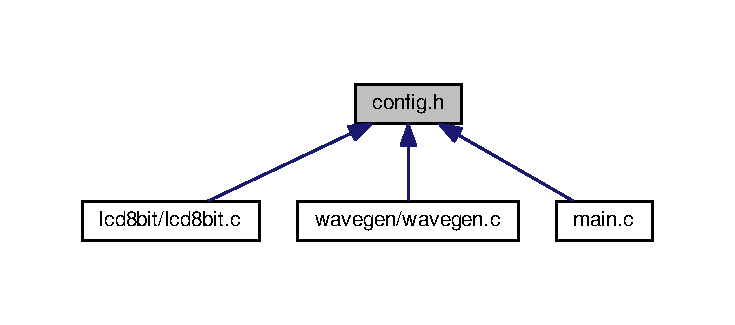
\includegraphics[width=350pt]{config_8h__dep__incl}
\end{center}
\end{figure}
\subsection*{Macros}
\begin{DoxyCompactItemize}
\item 
\#define \hyperlink{config_8h_a43bafb28b29491ec7f871319b5a3b2f8}{F\-\_\-\-C\-P\-U}~32000000\-U\-L
\end{DoxyCompactItemize}


\subsection{Macro Definition Documentation}
\hypertarget{config_8h_a43bafb28b29491ec7f871319b5a3b2f8}{\index{config.\-h@{config.\-h}!F\-\_\-\-C\-P\-U@{F\-\_\-\-C\-P\-U}}
\index{F\-\_\-\-C\-P\-U@{F\-\_\-\-C\-P\-U}!config.h@{config.\-h}}
\subsubsection[{F\-\_\-\-C\-P\-U}]{\setlength{\rightskip}{0pt plus 5cm}\#define F\-\_\-\-C\-P\-U~32000000\-U\-L}}\label{config_8h_a43bafb28b29491ec7f871319b5a3b2f8}

\hypertarget{keyboard_8c}{\section{keyboard/keyboard.c File Reference}
\label{keyboard_8c}\index{keyboard/keyboard.\-c@{keyboard/keyboard.\-c}}
}
{\ttfamily \#include \char`\"{}keyboard.\-h\char`\"{}}\\*
Include dependency graph for keyboard.\-c\-:\nopagebreak
\begin{figure}[H]
\begin{center}
\leavevmode
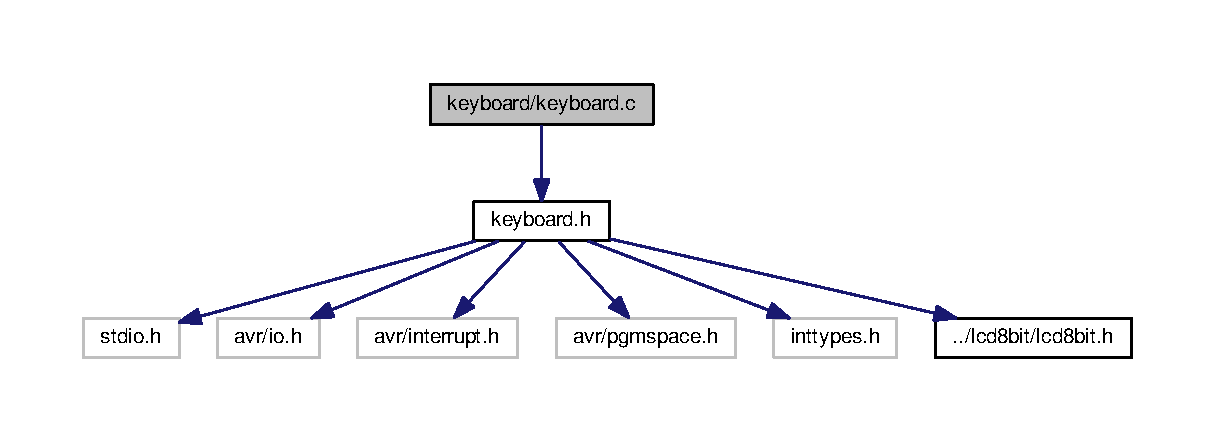
\includegraphics[width=350pt]{keyboard_8c__incl}
\end{center}
\end{figure}
\subsection*{Functions}
\begin{DoxyCompactItemize}
\item 
\hyperlink{keyboard_8c_aeaf658ec243c86cedf6953943cacfa6c}{I\-S\-R} (P\-O\-R\-T\-F\-\_\-\-I\-N\-T1\-\_\-vect)
\begin{DoxyCompactList}\small\item\em Interrupt service routine for P\-O\-R\-T\-F. \end{DoxyCompactList}\item 
void \hyperlink{keyboard_8c_a12e80295bc304d42073ca130ff9a9500}{keyboard\-\_\-clock\-\_\-init} (void)
\begin{DoxyCompactList}\small\item\em Initialiaze the clock to be 32\-Mhz. \end{DoxyCompactList}\item 
char \hyperlink{keyboard_8c_a0d8cfaf4d0e76cc5ecb09681adac3ef3}{keyboard\-\_\-render\-\_\-scan\-\_\-code} (uint8\-\_\-t data)
\item 
uint8\-\_\-t \hyperlink{keyboard_8c_a7060d775150320db57889d2659bb6284}{keyboard\-\_\-read\-\_\-char} ()
\item 
void \hyperlink{keyboard_8c_aaeb4e4a3c4813ee1efc6b98bba9ec781}{keyboard\-\_\-init} ()
\begin{DoxyCompactList}\small\item\em This function initialiazes the ports on the P\-S/2 port Sets up timer interrupts for P\-O\-R\-T\-F. \end{DoxyCompactList}\end{DoxyCompactItemize}
\subsection*{Variables}
\begin{DoxyCompactItemize}
\item 
char \hyperlink{keyboard_8c_ab51051b9acefccd468cdbd407c826fb0}{st} \mbox{[}20\mbox{]} =\char`\"{} \char`\"{}
\item 
volatile uint8\-\_\-t \hyperlink{keyboard_8c_ac6271798c92bfb95295c0eb43ad1f8a5}{kbd\-\_\-data}
\item 
volatile uint8\-\_\-t \hyperlink{keyboard_8c_a2076b44e14575d889c509d93df4e3ad2}{char\-\_\-waiting}
\item 
uint8\-\_\-t \hyperlink{keyboard_8c_a4962713018c207c653a60b1ec9554b52}{started}
\item 
uint8\-\_\-t \hyperlink{keyboard_8c_a3638028601cbd7e3383db0fe214e6c9b}{bit\-\_\-count}
\item 
uint8\-\_\-t \hyperlink{keyboard_8c_a28ac534ad4b71a6f265826746888e43e}{shift}
\item 
uint8\-\_\-t \hyperlink{keyboard_8c_ade2e2c50ad5f47ed8904d123c732d5a6}{caps\-\_\-lock}
\item 
uint8\-\_\-t \hyperlink{keyboard_8c_acd53bef429b3afe798b7228806e6e294}{extended}
\item 
uint8\-\_\-t \hyperlink{keyboard_8c_add4c887e71286ff439152f14a491d84b}{release}
\item 
const char keymap\mbox{[}128\mbox{]} \hyperlink{keyboard_8c_af786df5d8361570448476c5ec3d9e6e2}{P\-R\-O\-G\-M\-E\-M} = \{'?','?','?','?','?','?','?','?','?','?','?','?','?','?','?','?','?','?','?','?','?','q','1','?','?','?','z','s','a','w','2','?','?','c','x','d','e','4','3','?','?',' ','v','f','t','r','5','?','?','n','b','h','\hyperlink{list_8c_a71867e609034d4dbd6d0ad8d84540e59}{g}','y','6','?','?','?','m','j','u','7','8','?','?','?','k','i','o','0','9','?','?','?','?','l','?','p','?','?','?','?','?','?','?','?','?','?','?','?','?','?','?','?','?','?','?','?','?','?','?','?','?','?','?','?','?','?','?','?','?','?','?','?','?','?','?','?','?','?','?','?','?','?','?','?','?','?'\}
\begin{DoxyCompactList}\small\item\em include for P\-S/2 to A\-S\-C\-I\-I mapping \end{DoxyCompactList}\end{DoxyCompactItemize}


\subsection{Function Documentation}
\hypertarget{keyboard_8c_aeaf658ec243c86cedf6953943cacfa6c}{\index{keyboard.\-c@{keyboard.\-c}!I\-S\-R@{I\-S\-R}}
\index{I\-S\-R@{I\-S\-R}!keyboard.c@{keyboard.\-c}}
\subsubsection[{I\-S\-R}]{\setlength{\rightskip}{0pt plus 5cm}I\-S\-R (
\begin{DoxyParamCaption}
\item[{P\-O\-R\-T\-F\-\_\-\-I\-N\-T1\-\_\-vect}]{}
\end{DoxyParamCaption}
)}}\label{keyboard_8c_aeaf658ec243c86cedf6953943cacfa6c}


Interrupt service routine for P\-O\-R\-T\-F. 

Triggered when P\-O\-R\-T\-F pin 2 transitions from high to low. Handles P\-S/2 clock input and reads data in bit by bit. 

References bit\-\_\-count, char\-\_\-waiting, K\-B\-\_\-\-C\-L\-K, K\-B\-\_\-\-D\-A\-T\-A, K\-B\-\_\-\-P\-O\-R\-T, kbd\-\_\-data, release, shift, and started.

\hypertarget{keyboard_8c_a12e80295bc304d42073ca130ff9a9500}{\index{keyboard.\-c@{keyboard.\-c}!keyboard\-\_\-clock\-\_\-init@{keyboard\-\_\-clock\-\_\-init}}
\index{keyboard\-\_\-clock\-\_\-init@{keyboard\-\_\-clock\-\_\-init}!keyboard.c@{keyboard.\-c}}
\subsubsection[{keyboard\-\_\-clock\-\_\-init}]{\setlength{\rightskip}{0pt plus 5cm}void keyboard\-\_\-clock\-\_\-init (
\begin{DoxyParamCaption}
\item[{void}]{}
\end{DoxyParamCaption}
)}}\label{keyboard_8c_a12e80295bc304d42073ca130ff9a9500}


Initialiaze the clock to be 32\-Mhz. 

\hypertarget{keyboard_8c_aaeb4e4a3c4813ee1efc6b98bba9ec781}{\index{keyboard.\-c@{keyboard.\-c}!keyboard\-\_\-init@{keyboard\-\_\-init}}
\index{keyboard\-\_\-init@{keyboard\-\_\-init}!keyboard.c@{keyboard.\-c}}
\subsubsection[{keyboard\-\_\-init}]{\setlength{\rightskip}{0pt plus 5cm}void keyboard\-\_\-init (
\begin{DoxyParamCaption}
{}
\end{DoxyParamCaption}
)}}\label{keyboard_8c_aaeb4e4a3c4813ee1efc6b98bba9ec781}


This function initialiazes the ports on the P\-S/2 port Sets up timer interrupts for P\-O\-R\-T\-F. 

Make this interrupt medium level so it is higher priority than the timer interrupts!

References bit\-\_\-count, K\-B\-\_\-\-C\-L\-K, K\-B\-\_\-\-D\-A\-T\-A, K\-B\-\_\-\-P\-O\-R\-T, kbd\-\_\-data, and started.



Referenced by main().

\hypertarget{keyboard_8c_a7060d775150320db57889d2659bb6284}{\index{keyboard.\-c@{keyboard.\-c}!keyboard\-\_\-read\-\_\-char@{keyboard\-\_\-read\-\_\-char}}
\index{keyboard\-\_\-read\-\_\-char@{keyboard\-\_\-read\-\_\-char}!keyboard.c@{keyboard.\-c}}
\subsubsection[{keyboard\-\_\-read\-\_\-char}]{\setlength{\rightskip}{0pt plus 5cm}uint8\-\_\-t keyboard\-\_\-read\-\_\-char (
\begin{DoxyParamCaption}
{}
\end{DoxyParamCaption}
)}}\label{keyboard_8c_a7060d775150320db57889d2659bb6284}


References char\-\_\-waiting, kbd\-\_\-data, and release.



Referenced by main().

\hypertarget{keyboard_8c_a0d8cfaf4d0e76cc5ecb09681adac3ef3}{\index{keyboard.\-c@{keyboard.\-c}!keyboard\-\_\-render\-\_\-scan\-\_\-code@{keyboard\-\_\-render\-\_\-scan\-\_\-code}}
\index{keyboard\-\_\-render\-\_\-scan\-\_\-code@{keyboard\-\_\-render\-\_\-scan\-\_\-code}!keyboard.c@{keyboard.\-c}}
\subsubsection[{keyboard\-\_\-render\-\_\-scan\-\_\-code}]{\setlength{\rightskip}{0pt plus 5cm}char keyboard\-\_\-render\-\_\-scan\-\_\-code (
\begin{DoxyParamCaption}
\item[{uint8\-\_\-t}]{data}
\end{DoxyParamCaption}
)}}\label{keyboard_8c_a0d8cfaf4d0e76cc5ecb09681adac3ef3}


References shift.



Referenced by main().



\subsection{Variable Documentation}
\hypertarget{keyboard_8c_a3638028601cbd7e3383db0fe214e6c9b}{\index{keyboard.\-c@{keyboard.\-c}!bit\-\_\-count@{bit\-\_\-count}}
\index{bit\-\_\-count@{bit\-\_\-count}!keyboard.c@{keyboard.\-c}}
\subsubsection[{bit\-\_\-count}]{\setlength{\rightskip}{0pt plus 5cm}uint8\-\_\-t bit\-\_\-count}}\label{keyboard_8c_a3638028601cbd7e3383db0fe214e6c9b}


Referenced by I\-S\-R(), and keyboard\-\_\-init().

\hypertarget{keyboard_8c_ade2e2c50ad5f47ed8904d123c732d5a6}{\index{keyboard.\-c@{keyboard.\-c}!caps\-\_\-lock@{caps\-\_\-lock}}
\index{caps\-\_\-lock@{caps\-\_\-lock}!keyboard.c@{keyboard.\-c}}
\subsubsection[{caps\-\_\-lock}]{\setlength{\rightskip}{0pt plus 5cm}uint8\-\_\-t caps\-\_\-lock}}\label{keyboard_8c_ade2e2c50ad5f47ed8904d123c732d5a6}
\hypertarget{keyboard_8c_a2076b44e14575d889c509d93df4e3ad2}{\index{keyboard.\-c@{keyboard.\-c}!char\-\_\-waiting@{char\-\_\-waiting}}
\index{char\-\_\-waiting@{char\-\_\-waiting}!keyboard.c@{keyboard.\-c}}
\subsubsection[{char\-\_\-waiting}]{\setlength{\rightskip}{0pt plus 5cm}volatile uint8\-\_\-t char\-\_\-waiting}}\label{keyboard_8c_a2076b44e14575d889c509d93df4e3ad2}


Referenced by I\-S\-R(), keyboard\-\_\-read\-\_\-char(), and main().

\hypertarget{keyboard_8c_acd53bef429b3afe798b7228806e6e294}{\index{keyboard.\-c@{keyboard.\-c}!extended@{extended}}
\index{extended@{extended}!keyboard.c@{keyboard.\-c}}
\subsubsection[{extended}]{\setlength{\rightskip}{0pt plus 5cm}uint8\-\_\-t extended}}\label{keyboard_8c_acd53bef429b3afe798b7228806e6e294}
\hypertarget{keyboard_8c_ac6271798c92bfb95295c0eb43ad1f8a5}{\index{keyboard.\-c@{keyboard.\-c}!kbd\-\_\-data@{kbd\-\_\-data}}
\index{kbd\-\_\-data@{kbd\-\_\-data}!keyboard.c@{keyboard.\-c}}
\subsubsection[{kbd\-\_\-data}]{\setlength{\rightskip}{0pt plus 5cm}volatile uint8\-\_\-t kbd\-\_\-data}}\label{keyboard_8c_ac6271798c92bfb95295c0eb43ad1f8a5}


Referenced by I\-S\-R(), keyboard\-\_\-init(), and keyboard\-\_\-read\-\_\-char().

\hypertarget{keyboard_8c_af786df5d8361570448476c5ec3d9e6e2}{\index{keyboard.\-c@{keyboard.\-c}!P\-R\-O\-G\-M\-E\-M@{P\-R\-O\-G\-M\-E\-M}}
\index{P\-R\-O\-G\-M\-E\-M@{P\-R\-O\-G\-M\-E\-M}!keyboard.c@{keyboard.\-c}}
\subsubsection[{P\-R\-O\-G\-M\-E\-M}]{\setlength{\rightskip}{0pt plus 5cm}const char keymap \mbox{[}128\mbox{]} P\-R\-O\-G\-M\-E\-M = \{'?','?','?','?','?','?','?','?','?','?','?','?','?','?','?','?','?','?','?','?','?','q','1','?','?','?','z','s','a','w','2','?','?','c','x','d','e','4','3','?','?',' ','v','f','t','r','5','?','?','n','b','h','{\bf g}','y','6','?','?','?','m','j','u','7','8','?','?','?','k','i','o','0','9','?','?','?','?','l','?','p','?','?','?','?','?','?','?','?','?','?','?','?','?','?','?','?','?','?','?','?','?','?','?','?','?','?','?','?','?','?','?','?','?','?','?','?','?','?','?','?','?','?','?','?','?','?','?','?','?','?'\}}}\label{keyboard_8c_af786df5d8361570448476c5ec3d9e6e2}


include for P\-S/2 to A\-S\-C\-I\-I mapping 

\hypertarget{keyboard_8c_add4c887e71286ff439152f14a491d84b}{\index{keyboard.\-c@{keyboard.\-c}!release@{release}}
\index{release@{release}!keyboard.c@{keyboard.\-c}}
\subsubsection[{release}]{\setlength{\rightskip}{0pt plus 5cm}uint8\-\_\-t release}}\label{keyboard_8c_add4c887e71286ff439152f14a491d84b}


Referenced by I\-S\-R(), keyboard\-\_\-read\-\_\-char(), and main().

\hypertarget{keyboard_8c_a28ac534ad4b71a6f265826746888e43e}{\index{keyboard.\-c@{keyboard.\-c}!shift@{shift}}
\index{shift@{shift}!keyboard.c@{keyboard.\-c}}
\subsubsection[{shift}]{\setlength{\rightskip}{0pt plus 5cm}uint8\-\_\-t shift}}\label{keyboard_8c_a28ac534ad4b71a6f265826746888e43e}


Referenced by I\-S\-R(), and keyboard\-\_\-render\-\_\-scan\-\_\-code().

\hypertarget{keyboard_8c_ab51051b9acefccd468cdbd407c826fb0}{\index{keyboard.\-c@{keyboard.\-c}!st@{st}}
\index{st@{st}!keyboard.c@{keyboard.\-c}}
\subsubsection[{st}]{\setlength{\rightskip}{0pt plus 5cm}char st\mbox{[}20\mbox{]} =\char`\"{} \char`\"{}}}\label{keyboard_8c_ab51051b9acefccd468cdbd407c826fb0}
\hypertarget{keyboard_8c_a4962713018c207c653a60b1ec9554b52}{\index{keyboard.\-c@{keyboard.\-c}!started@{started}}
\index{started@{started}!keyboard.c@{keyboard.\-c}}
\subsubsection[{started}]{\setlength{\rightskip}{0pt plus 5cm}uint8\-\_\-t started}}\label{keyboard_8c_a4962713018c207c653a60b1ec9554b52}


Referenced by I\-S\-R(), and keyboard\-\_\-init().


\hypertarget{keyboard_8h}{\section{keyboard/keyboard.h File Reference}
\label{keyboard_8h}\index{keyboard/keyboard.\-h@{keyboard/keyboard.\-h}}
}
{\ttfamily \#include $<$stdio.\-h$>$}\\*
{\ttfamily \#include $<$avr/io.\-h$>$}\\*
{\ttfamily \#include $<$avr/interrupt.\-h$>$}\\*
{\ttfamily \#include $<$avr/pgmspace.\-h$>$}\\*
{\ttfamily \#include $<$inttypes.\-h$>$}\\*
{\ttfamily \#include \char`\"{}../lcd8bit/lcd8bit.\-h\char`\"{}}\\*
Include dependency graph for keyboard.\-h\-:\nopagebreak
\begin{figure}[H]
\begin{center}
\leavevmode
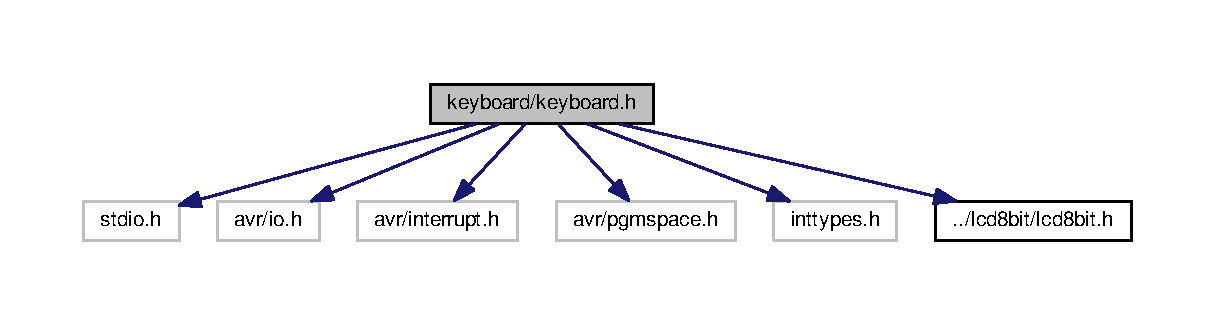
\includegraphics[width=350pt]{keyboard_8h__incl}
\end{center}
\end{figure}
This graph shows which files directly or indirectly include this file\-:\nopagebreak
\begin{figure}[H]
\begin{center}
\leavevmode
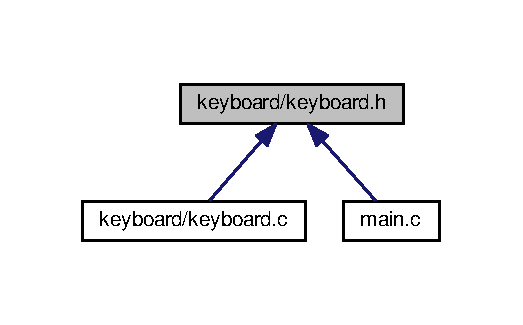
\includegraphics[width=251pt]{keyboard_8h__dep__incl}
\end{center}
\end{figure}
\subsection*{Macros}
\begin{DoxyCompactItemize}
\item 
\#define \hyperlink{keyboard_8h_a533f998159de957b1f91e571cda46b9c}{I\-N\-T\-E\-R\-R\-U\-P\-T\-\_\-\-P\-E\-R\-I\-O\-D}~512
\item 
\#define \hyperlink{keyboard_8h_abef1196c18f992aa76600b2fd4535bf9}{F\-I\-N\-T}~(\hyperlink{config_8h_a43bafb28b29491ec7f871319b5a3b2f8}{F\-\_\-\-C\-P\-U} / \hyperlink{~main_8c_a533f998159de957b1f91e571cda46b9c}{I\-N\-T\-E\-R\-R\-U\-P\-T\-\_\-\-P\-E\-R\-I\-O\-D})
\item 
\#define \hyperlink{keyboard_8h_a30588c5eca7c9cb6ebba02a0236f0119}{F\-S}~(\hyperlink{~main_8c_abef1196c18f992aa76600b2fd4535bf9}{F\-I\-N\-T})
\item 
\#define \hyperlink{keyboard_8h_a589673e7bbb27cd5ee1b6e977cb63d47}{K\-B\-\_\-\-C\-L\-K}~P\-I\-N2\-\_\-bm
\begin{DoxyCompactList}\small\item\em includes for lcd display library \end{DoxyCompactList}\item 
\#define \hyperlink{keyboard_8h_a2814188fded020b333e7d90454d61271}{K\-B\-\_\-\-D\-A\-T\-A}~P\-I\-N1\-\_\-bm
\begin{DoxyCompactList}\small\item\em set the keyboard data pin to P\-O\-R\-T\-F.\-1 \end{DoxyCompactList}\item 
\#define \hyperlink{keyboard_8h_acfa1f9e0b185e8d32bff74155a3ab4eb}{K\-B\-\_\-\-P\-O\-R\-T}~P\-O\-R\-T\-F
\begin{DoxyCompactList}\small\item\em define the keyboard port as P\-O\-R\-T\-F \end{DoxyCompactList}\end{DoxyCompactItemize}
\subsection*{Functions}
\begin{DoxyCompactItemize}
\item 
void \hyperlink{keyboard_8h_aaeb4e4a3c4813ee1efc6b98bba9ec781}{keyboard\-\_\-init} ()
\begin{DoxyCompactList}\small\item\em This function initialiazes the ports on the P\-S/2 port Sets up timer interrupts for P\-O\-R\-T\-F. \end{DoxyCompactList}\item 
char \hyperlink{keyboard_8h_a0d8cfaf4d0e76cc5ecb09681adac3ef3}{keyboard\-\_\-render\-\_\-scan\-\_\-code} (uint8\-\_\-t data)
\item 
uint8\-\_\-t \hyperlink{keyboard_8h_a7060d775150320db57889d2659bb6284}{keyboard\-\_\-read\-\_\-char} ()
\item 
void \hyperlink{keyboard_8h_a12e80295bc304d42073ca130ff9a9500}{keyboard\-\_\-clock\-\_\-init} (void)
\begin{DoxyCompactList}\small\item\em Initialiaze the clock to be 32\-Mhz. \end{DoxyCompactList}\end{DoxyCompactItemize}
\subsection*{Variables}
\begin{DoxyCompactItemize}
\item 
volatile uint8\-\_\-t \hyperlink{keyboard_8h_ac6271798c92bfb95295c0eb43ad1f8a5}{kbd\-\_\-data}
\item 
volatile uint8\-\_\-t \hyperlink{keyboard_8h_a2076b44e14575d889c509d93df4e3ad2}{char\-\_\-waiting}
\item 
uint8\-\_\-t \hyperlink{keyboard_8h_a4962713018c207c653a60b1ec9554b52}{started}
\item 
uint8\-\_\-t \hyperlink{keyboard_8h_a3638028601cbd7e3383db0fe214e6c9b}{bit\-\_\-count}
\item 
uint8\-\_\-t \hyperlink{keyboard_8h_a28ac534ad4b71a6f265826746888e43e}{shift}
\item 
uint8\-\_\-t \hyperlink{keyboard_8h_ade2e2c50ad5f47ed8904d123c732d5a6}{caps\-\_\-lock}
\item 
uint8\-\_\-t \hyperlink{keyboard_8h_acd53bef429b3afe798b7228806e6e294}{extended}
\item 
uint8\-\_\-t \hyperlink{keyboard_8h_add4c887e71286ff439152f14a491d84b}{release}
\end{DoxyCompactItemize}


\subsection{Macro Definition Documentation}
\hypertarget{keyboard_8h_abef1196c18f992aa76600b2fd4535bf9}{\index{keyboard.\-h@{keyboard.\-h}!F\-I\-N\-T@{F\-I\-N\-T}}
\index{F\-I\-N\-T@{F\-I\-N\-T}!keyboard.h@{keyboard.\-h}}
\subsubsection[{F\-I\-N\-T}]{\setlength{\rightskip}{0pt plus 5cm}\#define F\-I\-N\-T~({\bf F\-\_\-\-C\-P\-U} / {\bf I\-N\-T\-E\-R\-R\-U\-P\-T\-\_\-\-P\-E\-R\-I\-O\-D})}}\label{keyboard_8h_abef1196c18f992aa76600b2fd4535bf9}
\hypertarget{keyboard_8h_a30588c5eca7c9cb6ebba02a0236f0119}{\index{keyboard.\-h@{keyboard.\-h}!F\-S@{F\-S}}
\index{F\-S@{F\-S}!keyboard.h@{keyboard.\-h}}
\subsubsection[{F\-S}]{\setlength{\rightskip}{0pt plus 5cm}\#define F\-S~({\bf F\-I\-N\-T})}}\label{keyboard_8h_a30588c5eca7c9cb6ebba02a0236f0119}


Referenced by wavegen\-\_\-set\-Frequency(), and wavegen\-\_\-set\-Frequency2().

\hypertarget{keyboard_8h_a533f998159de957b1f91e571cda46b9c}{\index{keyboard.\-h@{keyboard.\-h}!I\-N\-T\-E\-R\-R\-U\-P\-T\-\_\-\-P\-E\-R\-I\-O\-D@{I\-N\-T\-E\-R\-R\-U\-P\-T\-\_\-\-P\-E\-R\-I\-O\-D}}
\index{I\-N\-T\-E\-R\-R\-U\-P\-T\-\_\-\-P\-E\-R\-I\-O\-D@{I\-N\-T\-E\-R\-R\-U\-P\-T\-\_\-\-P\-E\-R\-I\-O\-D}!keyboard.h@{keyboard.\-h}}
\subsubsection[{I\-N\-T\-E\-R\-R\-U\-P\-T\-\_\-\-P\-E\-R\-I\-O\-D}]{\setlength{\rightskip}{0pt plus 5cm}\#define I\-N\-T\-E\-R\-R\-U\-P\-T\-\_\-\-P\-E\-R\-I\-O\-D~512}}\label{keyboard_8h_a533f998159de957b1f91e571cda46b9c}
\hypertarget{keyboard_8h_a589673e7bbb27cd5ee1b6e977cb63d47}{\index{keyboard.\-h@{keyboard.\-h}!K\-B\-\_\-\-C\-L\-K@{K\-B\-\_\-\-C\-L\-K}}
\index{K\-B\-\_\-\-C\-L\-K@{K\-B\-\_\-\-C\-L\-K}!keyboard.h@{keyboard.\-h}}
\subsubsection[{K\-B\-\_\-\-C\-L\-K}]{\setlength{\rightskip}{0pt plus 5cm}\#define K\-B\-\_\-\-C\-L\-K~P\-I\-N2\-\_\-bm}}\label{keyboard_8h_a589673e7bbb27cd5ee1b6e977cb63d47}


includes for lcd display library 

set the keyboard clock pin to P\-O\-R\-T\-F.\-2 

Referenced by I\-S\-R(), and keyboard\-\_\-init().

\hypertarget{keyboard_8h_a2814188fded020b333e7d90454d61271}{\index{keyboard.\-h@{keyboard.\-h}!K\-B\-\_\-\-D\-A\-T\-A@{K\-B\-\_\-\-D\-A\-T\-A}}
\index{K\-B\-\_\-\-D\-A\-T\-A@{K\-B\-\_\-\-D\-A\-T\-A}!keyboard.h@{keyboard.\-h}}
\subsubsection[{K\-B\-\_\-\-D\-A\-T\-A}]{\setlength{\rightskip}{0pt plus 5cm}\#define K\-B\-\_\-\-D\-A\-T\-A~P\-I\-N1\-\_\-bm}}\label{keyboard_8h_a2814188fded020b333e7d90454d61271}


set the keyboard data pin to P\-O\-R\-T\-F.\-1 



Referenced by I\-S\-R(), and keyboard\-\_\-init().

\hypertarget{keyboard_8h_acfa1f9e0b185e8d32bff74155a3ab4eb}{\index{keyboard.\-h@{keyboard.\-h}!K\-B\-\_\-\-P\-O\-R\-T@{K\-B\-\_\-\-P\-O\-R\-T}}
\index{K\-B\-\_\-\-P\-O\-R\-T@{K\-B\-\_\-\-P\-O\-R\-T}!keyboard.h@{keyboard.\-h}}
\subsubsection[{K\-B\-\_\-\-P\-O\-R\-T}]{\setlength{\rightskip}{0pt plus 5cm}\#define K\-B\-\_\-\-P\-O\-R\-T~P\-O\-R\-T\-F}}\label{keyboard_8h_acfa1f9e0b185e8d32bff74155a3ab4eb}


define the keyboard port as P\-O\-R\-T\-F 



Referenced by I\-S\-R(), and keyboard\-\_\-init().



\subsection{Function Documentation}
\hypertarget{keyboard_8h_a12e80295bc304d42073ca130ff9a9500}{\index{keyboard.\-h@{keyboard.\-h}!keyboard\-\_\-clock\-\_\-init@{keyboard\-\_\-clock\-\_\-init}}
\index{keyboard\-\_\-clock\-\_\-init@{keyboard\-\_\-clock\-\_\-init}!keyboard.h@{keyboard.\-h}}
\subsubsection[{keyboard\-\_\-clock\-\_\-init}]{\setlength{\rightskip}{0pt plus 5cm}void keyboard\-\_\-clock\-\_\-init (
\begin{DoxyParamCaption}
\item[{void}]{}
\end{DoxyParamCaption}
)}}\label{keyboard_8h_a12e80295bc304d42073ca130ff9a9500}


Initialiaze the clock to be 32\-Mhz. 

\hypertarget{keyboard_8h_aaeb4e4a3c4813ee1efc6b98bba9ec781}{\index{keyboard.\-h@{keyboard.\-h}!keyboard\-\_\-init@{keyboard\-\_\-init}}
\index{keyboard\-\_\-init@{keyboard\-\_\-init}!keyboard.h@{keyboard.\-h}}
\subsubsection[{keyboard\-\_\-init}]{\setlength{\rightskip}{0pt plus 5cm}void keyboard\-\_\-init (
\begin{DoxyParamCaption}
{}
\end{DoxyParamCaption}
)}}\label{keyboard_8h_aaeb4e4a3c4813ee1efc6b98bba9ec781}


This function initialiazes the ports on the P\-S/2 port Sets up timer interrupts for P\-O\-R\-T\-F. 

Make this interrupt medium level so it is higher priority than the timer interrupts!

References bit\-\_\-count, K\-B\-\_\-\-C\-L\-K, K\-B\-\_\-\-D\-A\-T\-A, K\-B\-\_\-\-P\-O\-R\-T, kbd\-\_\-data, and started.



Referenced by main().

\hypertarget{keyboard_8h_a7060d775150320db57889d2659bb6284}{\index{keyboard.\-h@{keyboard.\-h}!keyboard\-\_\-read\-\_\-char@{keyboard\-\_\-read\-\_\-char}}
\index{keyboard\-\_\-read\-\_\-char@{keyboard\-\_\-read\-\_\-char}!keyboard.h@{keyboard.\-h}}
\subsubsection[{keyboard\-\_\-read\-\_\-char}]{\setlength{\rightskip}{0pt plus 5cm}uint8\-\_\-t keyboard\-\_\-read\-\_\-char (
\begin{DoxyParamCaption}
{}
\end{DoxyParamCaption}
)}}\label{keyboard_8h_a7060d775150320db57889d2659bb6284}


References char\-\_\-waiting, kbd\-\_\-data, and release.



Referenced by main().

\hypertarget{keyboard_8h_a0d8cfaf4d0e76cc5ecb09681adac3ef3}{\index{keyboard.\-h@{keyboard.\-h}!keyboard\-\_\-render\-\_\-scan\-\_\-code@{keyboard\-\_\-render\-\_\-scan\-\_\-code}}
\index{keyboard\-\_\-render\-\_\-scan\-\_\-code@{keyboard\-\_\-render\-\_\-scan\-\_\-code}!keyboard.h@{keyboard.\-h}}
\subsubsection[{keyboard\-\_\-render\-\_\-scan\-\_\-code}]{\setlength{\rightskip}{0pt plus 5cm}char keyboard\-\_\-render\-\_\-scan\-\_\-code (
\begin{DoxyParamCaption}
\item[{uint8\-\_\-t}]{data}
\end{DoxyParamCaption}
)}}\label{keyboard_8h_a0d8cfaf4d0e76cc5ecb09681adac3ef3}


References shift.



Referenced by main().



\subsection{Variable Documentation}
\hypertarget{keyboard_8h_a3638028601cbd7e3383db0fe214e6c9b}{\index{keyboard.\-h@{keyboard.\-h}!bit\-\_\-count@{bit\-\_\-count}}
\index{bit\-\_\-count@{bit\-\_\-count}!keyboard.h@{keyboard.\-h}}
\subsubsection[{bit\-\_\-count}]{\setlength{\rightskip}{0pt plus 5cm}uint8\-\_\-t bit\-\_\-count}}\label{keyboard_8h_a3638028601cbd7e3383db0fe214e6c9b}
\hypertarget{keyboard_8h_ade2e2c50ad5f47ed8904d123c732d5a6}{\index{keyboard.\-h@{keyboard.\-h}!caps\-\_\-lock@{caps\-\_\-lock}}
\index{caps\-\_\-lock@{caps\-\_\-lock}!keyboard.h@{keyboard.\-h}}
\subsubsection[{caps\-\_\-lock}]{\setlength{\rightskip}{0pt plus 5cm}uint8\-\_\-t caps\-\_\-lock}}\label{keyboard_8h_ade2e2c50ad5f47ed8904d123c732d5a6}
\hypertarget{keyboard_8h_a2076b44e14575d889c509d93df4e3ad2}{\index{keyboard.\-h@{keyboard.\-h}!char\-\_\-waiting@{char\-\_\-waiting}}
\index{char\-\_\-waiting@{char\-\_\-waiting}!keyboard.h@{keyboard.\-h}}
\subsubsection[{char\-\_\-waiting}]{\setlength{\rightskip}{0pt plus 5cm}volatile uint8\-\_\-t char\-\_\-waiting}}\label{keyboard_8h_a2076b44e14575d889c509d93df4e3ad2}
\hypertarget{keyboard_8h_acd53bef429b3afe798b7228806e6e294}{\index{keyboard.\-h@{keyboard.\-h}!extended@{extended}}
\index{extended@{extended}!keyboard.h@{keyboard.\-h}}
\subsubsection[{extended}]{\setlength{\rightskip}{0pt plus 5cm}uint8\-\_\-t extended}}\label{keyboard_8h_acd53bef429b3afe798b7228806e6e294}
\hypertarget{keyboard_8h_ac6271798c92bfb95295c0eb43ad1f8a5}{\index{keyboard.\-h@{keyboard.\-h}!kbd\-\_\-data@{kbd\-\_\-data}}
\index{kbd\-\_\-data@{kbd\-\_\-data}!keyboard.h@{keyboard.\-h}}
\subsubsection[{kbd\-\_\-data}]{\setlength{\rightskip}{0pt plus 5cm}volatile uint8\-\_\-t kbd\-\_\-data}}\label{keyboard_8h_ac6271798c92bfb95295c0eb43ad1f8a5}
\hypertarget{keyboard_8h_add4c887e71286ff439152f14a491d84b}{\index{keyboard.\-h@{keyboard.\-h}!release@{release}}
\index{release@{release}!keyboard.h@{keyboard.\-h}}
\subsubsection[{release}]{\setlength{\rightskip}{0pt plus 5cm}uint8\-\_\-t release}}\label{keyboard_8h_add4c887e71286ff439152f14a491d84b}
\hypertarget{keyboard_8h_a28ac534ad4b71a6f265826746888e43e}{\index{keyboard.\-h@{keyboard.\-h}!shift@{shift}}
\index{shift@{shift}!keyboard.h@{keyboard.\-h}}
\subsubsection[{shift}]{\setlength{\rightskip}{0pt plus 5cm}uint8\-\_\-t shift}}\label{keyboard_8h_a28ac534ad4b71a6f265826746888e43e}
\hypertarget{keyboard_8h_a4962713018c207c653a60b1ec9554b52}{\index{keyboard.\-h@{keyboard.\-h}!started@{started}}
\index{started@{started}!keyboard.h@{keyboard.\-h}}
\subsubsection[{started}]{\setlength{\rightskip}{0pt plus 5cm}uint8\-\_\-t started}}\label{keyboard_8h_a4962713018c207c653a60b1ec9554b52}

\hypertarget{keymap_8h}{\section{keyboard/keymap.h File Reference}
\label{keymap_8h}\index{keyboard/keymap.\-h@{keyboard/keymap.\-h}}
}

\hypertarget{lcd8bit_8c}{\section{lcd8bit/lcd8bit.c File Reference}
\label{lcd8bit_8c}\index{lcd8bit/lcd8bit.\-c@{lcd8bit/lcd8bit.\-c}}
}
{\ttfamily \#include \char`\"{}../config.\-h\char`\"{}}\\*
{\ttfamily \#include $<$avr/io.\-h$>$}\\*
{\ttfamily \#include $<$avr/pgmspace.\-h$>$}\\*
{\ttfamily \#include $<$util/delay.\-h$>$}\\*
{\ttfamily \#include $<$stdio.\-h$>$}\\*
{\ttfamily \#include \char`\"{}lcd8bit.\-h\char`\"{}}\\*
Include dependency graph for lcd8bit.\-c\-:\nopagebreak
\begin{figure}[H]
\begin{center}
\leavevmode
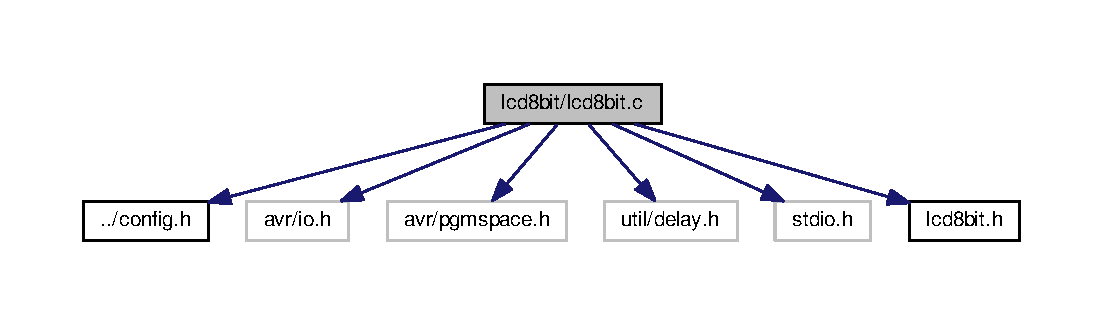
\includegraphics[width=350pt]{lcd8bit_8c__incl}
\end{center}
\end{figure}
\subsection*{Macros}
\begin{DoxyCompactItemize}
\item 
\#define \hyperlink{lcd8bit_8c_ab0c169c959c5be67954c866776329563}{D\-A\-T\-A\-\_\-\-P\-O\-R\-T}~P\-O\-R\-T\-B
\item 
\#define \hyperlink{lcd8bit_8c_a4781e073871c6f27f89b9463ad3a4ed1}{L\-C\-D\-\_\-\-R\-S}~P\-I\-N0\-\_\-bm    /$\ast$ R\-S on pin P\-B3 $\ast$/
\item 
\#define \hyperlink{lcd8bit_8c_a6ec15b1e813d1f56d2eb644a127e5d49}{L\-C\-D\-\_\-\-E}~P\-I\-N1\-\_\-bm    /$\ast$ E on pin P\-B1 $\ast$/
\item 
\#define \hyperlink{lcd8bit_8c_a18b1a802fdc6371ca9ea8219ab62f219}{C\-O\-M\-M\-\_\-\-P\-O\-R\-T}~P\-O\-R\-T\-A
\end{DoxyCompactItemize}
\subsection*{Functions}
\begin{DoxyCompactItemize}
\item 
void \hyperlink{lcd8bit_8c_a9d0f278e2fa5d8921d3a4fdd508a561e}{lcd\-\_\-set\-\_\-write\-\_\-instruction} ()
\item 
void \hyperlink{lcd8bit_8c_ad55e5c04e2a5354bfd4840be5e0eb5d1}{lcd\-\_\-set\-\_\-write\-\_\-data} ()
\item 
void \hyperlink{lcd8bit_8c_aef7fba4025d73ad60e375357e557bca3}{lcd\-\_\-write\-\_\-byte} (char c)
\item 
void \hyperlink{lcd8bit_8c_a88fdc90276b48773630acfc4525ff0db}{lcd\-\_\-clear\-\_\-and\-\_\-home} ()
\item 
void \hyperlink{lcd8bit_8c_a60675105b93bba6762aaab88d732365a}{lcd\-\_\-home} ()
\item 
void \hyperlink{lcd8bit_8c_affc4cf9b640d7c72fcb1e8be36c0183c}{lcd\-\_\-goto} (uint8\-\_\-t line, uint8\-\_\-t pos)
\item 
void \hyperlink{lcd8bit_8c_a8752d4e091188fcb07bbc9ae3c496e95}{lcd\-\_\-line\-\_\-one} ()
\item 
void \hyperlink{lcd8bit_8c_aa0b44a03031cc3639604de620e426021}{lcd\-\_\-line\-\_\-two} ()
\item 
void \hyperlink{lcd8bit_8c_a082c749307f206b15a9cbeb775b03b5c}{lcd\-\_\-write\-\_\-data} (char c)
\item 
void \hyperlink{lcd8bit_8c_a348a0350888f0a9bc01ed290423e2af8}{lcd\-\_\-write\-\_\-string} (char $\ast$x, uint8\-\_\-t len)
\item 
void \hyperlink{lcd8bit_8c_a9aa8378a804ddb51f770bd01665df653}{lcd\-\_\-write\-\_\-string\-\_\-0} (char $\ast$x)
\item 
void \hyperlink{lcd8bit_8c_a39cdfea82914e968ea1dbf7a8c6c9f9e}{lcd\-\_\-write\-\_\-string\-\_\-p} (const char $\ast$s)
\item 
void \hyperlink{lcd8bit_8c_ac23e73124dc9fabae95671fe71d074a6}{lcd\-\_\-init} ()
\end{DoxyCompactItemize}


\subsection{Macro Definition Documentation}
\hypertarget{lcd8bit_8c_a18b1a802fdc6371ca9ea8219ab62f219}{\index{lcd8bit.\-c@{lcd8bit.\-c}!C\-O\-M\-M\-\_\-\-P\-O\-R\-T@{C\-O\-M\-M\-\_\-\-P\-O\-R\-T}}
\index{C\-O\-M\-M\-\_\-\-P\-O\-R\-T@{C\-O\-M\-M\-\_\-\-P\-O\-R\-T}!lcd8bit.c@{lcd8bit.\-c}}
\subsubsection[{C\-O\-M\-M\-\_\-\-P\-O\-R\-T}]{\setlength{\rightskip}{0pt plus 5cm}\#define C\-O\-M\-M\-\_\-\-P\-O\-R\-T~P\-O\-R\-T\-A}}\label{lcd8bit_8c_a18b1a802fdc6371ca9ea8219ab62f219}


Referenced by lcd\-\_\-init(), lcd\-\_\-set\-\_\-write\-\_\-data(), lcd\-\_\-set\-\_\-write\-\_\-instruction(), and lcd\-\_\-write\-\_\-byte().

\hypertarget{lcd8bit_8c_ab0c169c959c5be67954c866776329563}{\index{lcd8bit.\-c@{lcd8bit.\-c}!D\-A\-T\-A\-\_\-\-P\-O\-R\-T@{D\-A\-T\-A\-\_\-\-P\-O\-R\-T}}
\index{D\-A\-T\-A\-\_\-\-P\-O\-R\-T@{D\-A\-T\-A\-\_\-\-P\-O\-R\-T}!lcd8bit.c@{lcd8bit.\-c}}
\subsubsection[{D\-A\-T\-A\-\_\-\-P\-O\-R\-T}]{\setlength{\rightskip}{0pt plus 5cm}\#define D\-A\-T\-A\-\_\-\-P\-O\-R\-T~P\-O\-R\-T\-B}}\label{lcd8bit_8c_ab0c169c959c5be67954c866776329563}


Referenced by lcd\-\_\-init(), and lcd\-\_\-write\-\_\-byte().

\hypertarget{lcd8bit_8c_a6ec15b1e813d1f56d2eb644a127e5d49}{\index{lcd8bit.\-c@{lcd8bit.\-c}!L\-C\-D\-\_\-\-E@{L\-C\-D\-\_\-\-E}}
\index{L\-C\-D\-\_\-\-E@{L\-C\-D\-\_\-\-E}!lcd8bit.c@{lcd8bit.\-c}}
\subsubsection[{L\-C\-D\-\_\-\-E}]{\setlength{\rightskip}{0pt plus 5cm}\#define L\-C\-D\-\_\-\-E~P\-I\-N1\-\_\-bm    /$\ast$ E on pin P\-B1 $\ast$/}}\label{lcd8bit_8c_a6ec15b1e813d1f56d2eb644a127e5d49}


Referenced by lcd\-\_\-init(), and lcd\-\_\-write\-\_\-byte().

\hypertarget{lcd8bit_8c_a4781e073871c6f27f89b9463ad3a4ed1}{\index{lcd8bit.\-c@{lcd8bit.\-c}!L\-C\-D\-\_\-\-R\-S@{L\-C\-D\-\_\-\-R\-S}}
\index{L\-C\-D\-\_\-\-R\-S@{L\-C\-D\-\_\-\-R\-S}!lcd8bit.c@{lcd8bit.\-c}}
\subsubsection[{L\-C\-D\-\_\-\-R\-S}]{\setlength{\rightskip}{0pt plus 5cm}\#define L\-C\-D\-\_\-\-R\-S~P\-I\-N0\-\_\-bm    /$\ast$ R\-S on pin P\-B3 $\ast$/}}\label{lcd8bit_8c_a4781e073871c6f27f89b9463ad3a4ed1}


Referenced by lcd\-\_\-init(), lcd\-\_\-set\-\_\-write\-\_\-data(), and lcd\-\_\-set\-\_\-write\-\_\-instruction().



\subsection{Function Documentation}
\hypertarget{lcd8bit_8c_a88fdc90276b48773630acfc4525ff0db}{\index{lcd8bit.\-c@{lcd8bit.\-c}!lcd\-\_\-clear\-\_\-and\-\_\-home@{lcd\-\_\-clear\-\_\-and\-\_\-home}}
\index{lcd\-\_\-clear\-\_\-and\-\_\-home@{lcd\-\_\-clear\-\_\-and\-\_\-home}!lcd8bit.c@{lcd8bit.\-c}}
\subsubsection[{lcd\-\_\-clear\-\_\-and\-\_\-home}]{\setlength{\rightskip}{0pt plus 5cm}void lcd\-\_\-clear\-\_\-and\-\_\-home (
\begin{DoxyParamCaption}
{}
\end{DoxyParamCaption}
)}}\label{lcd8bit_8c_a88fdc90276b48773630acfc4525ff0db}


References lcd\-\_\-set\-\_\-write\-\_\-instruction(), and lcd\-\_\-write\-\_\-byte().



Referenced by die(), lcd\-\_\-init(), and main().



Here is the call graph for this function\-:
\nopagebreak
\begin{figure}[H]
\begin{center}
\leavevmode
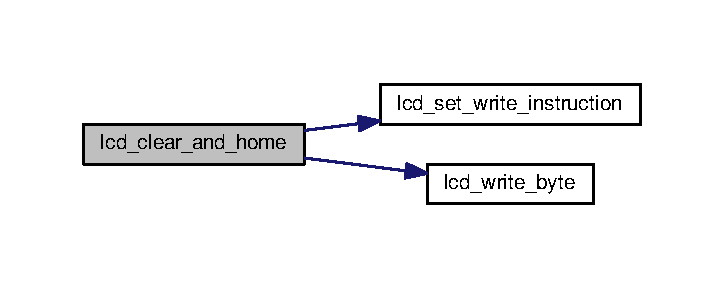
\includegraphics[width=348pt]{lcd8bit_8c_a88fdc90276b48773630acfc4525ff0db_cgraph}
\end{center}
\end{figure}


\hypertarget{lcd8bit_8c_affc4cf9b640d7c72fcb1e8be36c0183c}{\index{lcd8bit.\-c@{lcd8bit.\-c}!lcd\-\_\-goto@{lcd\-\_\-goto}}
\index{lcd\-\_\-goto@{lcd\-\_\-goto}!lcd8bit.c@{lcd8bit.\-c}}
\subsubsection[{lcd\-\_\-goto}]{\setlength{\rightskip}{0pt plus 5cm}void lcd\-\_\-goto (
\begin{DoxyParamCaption}
\item[{uint8\-\_\-t}]{line, }
\item[{uint8\-\_\-t}]{pos}
\end{DoxyParamCaption}
)}}\label{lcd8bit_8c_affc4cf9b640d7c72fcb1e8be36c0183c}


References lcd\-\_\-set\-\_\-write\-\_\-instruction(), and lcd\-\_\-write\-\_\-byte().



Referenced by lcd\-\_\-line\-\_\-one(), and lcd\-\_\-line\-\_\-two().



Here is the call graph for this function\-:
\nopagebreak
\begin{figure}[H]
\begin{center}
\leavevmode
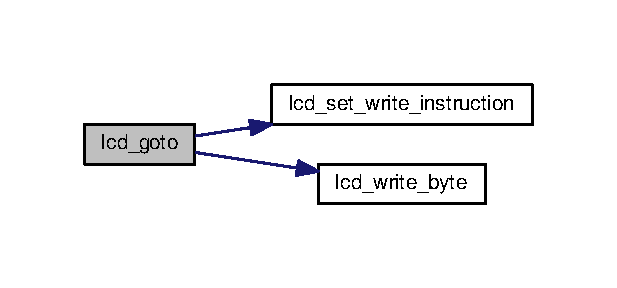
\includegraphics[width=296pt]{lcd8bit_8c_affc4cf9b640d7c72fcb1e8be36c0183c_cgraph}
\end{center}
\end{figure}


\hypertarget{lcd8bit_8c_a60675105b93bba6762aaab88d732365a}{\index{lcd8bit.\-c@{lcd8bit.\-c}!lcd\-\_\-home@{lcd\-\_\-home}}
\index{lcd\-\_\-home@{lcd\-\_\-home}!lcd8bit.c@{lcd8bit.\-c}}
\subsubsection[{lcd\-\_\-home}]{\setlength{\rightskip}{0pt plus 5cm}void lcd\-\_\-home (
\begin{DoxyParamCaption}
{}
\end{DoxyParamCaption}
)}}\label{lcd8bit_8c_a60675105b93bba6762aaab88d732365a}


References lcd\-\_\-set\-\_\-write\-\_\-instruction(), and lcd\-\_\-write\-\_\-byte().



Here is the call graph for this function\-:
\nopagebreak
\begin{figure}[H]
\begin{center}
\leavevmode
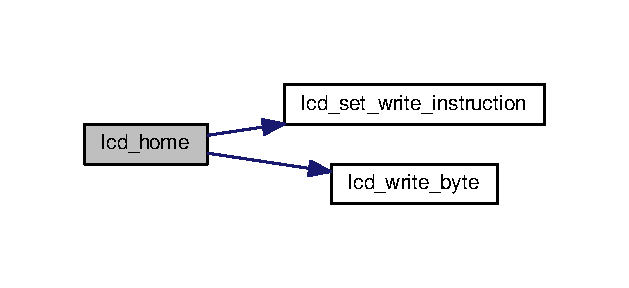
\includegraphics[width=302pt]{lcd8bit_8c_a60675105b93bba6762aaab88d732365a_cgraph}
\end{center}
\end{figure}


\hypertarget{lcd8bit_8c_ac23e73124dc9fabae95671fe71d074a6}{\index{lcd8bit.\-c@{lcd8bit.\-c}!lcd\-\_\-init@{lcd\-\_\-init}}
\index{lcd\-\_\-init@{lcd\-\_\-init}!lcd8bit.c@{lcd8bit.\-c}}
\subsubsection[{lcd\-\_\-init}]{\setlength{\rightskip}{0pt plus 5cm}void lcd\-\_\-init (
\begin{DoxyParamCaption}
{}
\end{DoxyParamCaption}
)}}\label{lcd8bit_8c_ac23e73124dc9fabae95671fe71d074a6}


References C\-O\-M\-M\-\_\-\-P\-O\-R\-T, D\-A\-T\-A\-\_\-\-P\-O\-R\-T, lcd\-\_\-clear\-\_\-and\-\_\-home(), L\-C\-D\-\_\-\-E, L\-C\-D\-\_\-\-R\-S, and lcd\-\_\-write\-\_\-byte().



Referenced by main().



Here is the call graph for this function\-:
\nopagebreak
\begin{figure}[H]
\begin{center}
\leavevmode
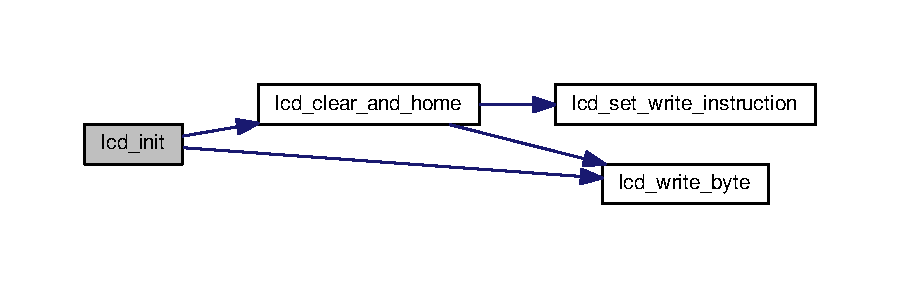
\includegraphics[width=350pt]{lcd8bit_8c_ac23e73124dc9fabae95671fe71d074a6_cgraph}
\end{center}
\end{figure}


\hypertarget{lcd8bit_8c_a8752d4e091188fcb07bbc9ae3c496e95}{\index{lcd8bit.\-c@{lcd8bit.\-c}!lcd\-\_\-line\-\_\-one@{lcd\-\_\-line\-\_\-one}}
\index{lcd\-\_\-line\-\_\-one@{lcd\-\_\-line\-\_\-one}!lcd8bit.c@{lcd8bit.\-c}}
\subsubsection[{lcd\-\_\-line\-\_\-one}]{\setlength{\rightskip}{0pt plus 5cm}void lcd\-\_\-line\-\_\-one (
\begin{DoxyParamCaption}
{}
\end{DoxyParamCaption}
)}}\label{lcd8bit_8c_a8752d4e091188fcb07bbc9ae3c496e95}


References lcd\-\_\-goto().



Referenced by die(), and main().



Here is the call graph for this function\-:
\nopagebreak
\begin{figure}[H]
\begin{center}
\leavevmode
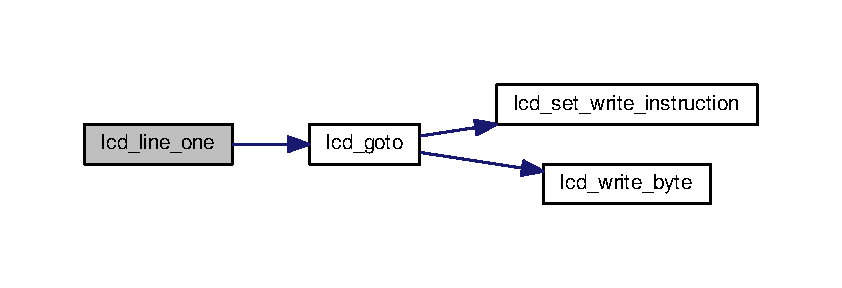
\includegraphics[width=350pt]{lcd8bit_8c_a8752d4e091188fcb07bbc9ae3c496e95_cgraph}
\end{center}
\end{figure}


\hypertarget{lcd8bit_8c_aa0b44a03031cc3639604de620e426021}{\index{lcd8bit.\-c@{lcd8bit.\-c}!lcd\-\_\-line\-\_\-two@{lcd\-\_\-line\-\_\-two}}
\index{lcd\-\_\-line\-\_\-two@{lcd\-\_\-line\-\_\-two}!lcd8bit.c@{lcd8bit.\-c}}
\subsubsection[{lcd\-\_\-line\-\_\-two}]{\setlength{\rightskip}{0pt plus 5cm}void lcd\-\_\-line\-\_\-two (
\begin{DoxyParamCaption}
{}
\end{DoxyParamCaption}
)}}\label{lcd8bit_8c_aa0b44a03031cc3639604de620e426021}


References lcd\-\_\-goto().



Referenced by die(), and main().



Here is the call graph for this function\-:
\nopagebreak
\begin{figure}[H]
\begin{center}
\leavevmode
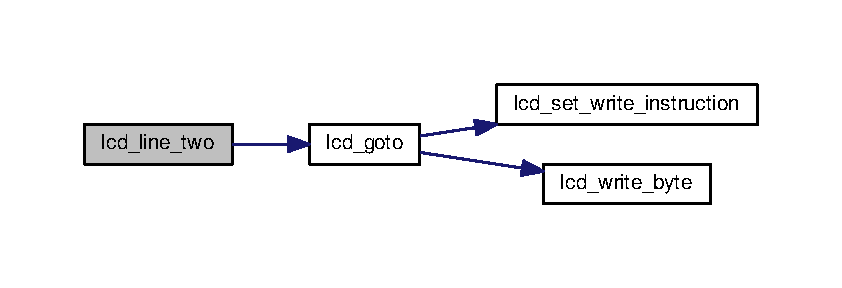
\includegraphics[width=350pt]{lcd8bit_8c_aa0b44a03031cc3639604de620e426021_cgraph}
\end{center}
\end{figure}


\hypertarget{lcd8bit_8c_ad55e5c04e2a5354bfd4840be5e0eb5d1}{\index{lcd8bit.\-c@{lcd8bit.\-c}!lcd\-\_\-set\-\_\-write\-\_\-data@{lcd\-\_\-set\-\_\-write\-\_\-data}}
\index{lcd\-\_\-set\-\_\-write\-\_\-data@{lcd\-\_\-set\-\_\-write\-\_\-data}!lcd8bit.c@{lcd8bit.\-c}}
\subsubsection[{lcd\-\_\-set\-\_\-write\-\_\-data}]{\setlength{\rightskip}{0pt plus 5cm}void lcd\-\_\-set\-\_\-write\-\_\-data (
\begin{DoxyParamCaption}
{}
\end{DoxyParamCaption}
)}}\label{lcd8bit_8c_ad55e5c04e2a5354bfd4840be5e0eb5d1}


References C\-O\-M\-M\-\_\-\-P\-O\-R\-T, and L\-C\-D\-\_\-\-R\-S.



Referenced by lcd\-\_\-write\-\_\-data().

\hypertarget{lcd8bit_8c_a9d0f278e2fa5d8921d3a4fdd508a561e}{\index{lcd8bit.\-c@{lcd8bit.\-c}!lcd\-\_\-set\-\_\-write\-\_\-instruction@{lcd\-\_\-set\-\_\-write\-\_\-instruction}}
\index{lcd\-\_\-set\-\_\-write\-\_\-instruction@{lcd\-\_\-set\-\_\-write\-\_\-instruction}!lcd8bit.c@{lcd8bit.\-c}}
\subsubsection[{lcd\-\_\-set\-\_\-write\-\_\-instruction}]{\setlength{\rightskip}{0pt plus 5cm}void lcd\-\_\-set\-\_\-write\-\_\-instruction (
\begin{DoxyParamCaption}
{}
\end{DoxyParamCaption}
)}}\label{lcd8bit_8c_a9d0f278e2fa5d8921d3a4fdd508a561e}


References C\-O\-M\-M\-\_\-\-P\-O\-R\-T, and L\-C\-D\-\_\-\-R\-S.



Referenced by lcd\-\_\-clear\-\_\-and\-\_\-home(), lcd\-\_\-goto(), and lcd\-\_\-home().

\hypertarget{lcd8bit_8c_aef7fba4025d73ad60e375357e557bca3}{\index{lcd8bit.\-c@{lcd8bit.\-c}!lcd\-\_\-write\-\_\-byte@{lcd\-\_\-write\-\_\-byte}}
\index{lcd\-\_\-write\-\_\-byte@{lcd\-\_\-write\-\_\-byte}!lcd8bit.c@{lcd8bit.\-c}}
\subsubsection[{lcd\-\_\-write\-\_\-byte}]{\setlength{\rightskip}{0pt plus 5cm}void lcd\-\_\-write\-\_\-byte (
\begin{DoxyParamCaption}
\item[{char}]{c}
\end{DoxyParamCaption}
)}}\label{lcd8bit_8c_aef7fba4025d73ad60e375357e557bca3}


References C\-O\-M\-M\-\_\-\-P\-O\-R\-T, D\-A\-T\-A\-\_\-\-P\-O\-R\-T, and L\-C\-D\-\_\-\-E.



Referenced by lcd\-\_\-clear\-\_\-and\-\_\-home(), lcd\-\_\-goto(), lcd\-\_\-home(), lcd\-\_\-init(), and lcd\-\_\-write\-\_\-data().

\hypertarget{lcd8bit_8c_a082c749307f206b15a9cbeb775b03b5c}{\index{lcd8bit.\-c@{lcd8bit.\-c}!lcd\-\_\-write\-\_\-data@{lcd\-\_\-write\-\_\-data}}
\index{lcd\-\_\-write\-\_\-data@{lcd\-\_\-write\-\_\-data}!lcd8bit.c@{lcd8bit.\-c}}
\subsubsection[{lcd\-\_\-write\-\_\-data}]{\setlength{\rightskip}{0pt plus 5cm}void lcd\-\_\-write\-\_\-data (
\begin{DoxyParamCaption}
\item[{char}]{c}
\end{DoxyParamCaption}
)}}\label{lcd8bit_8c_a082c749307f206b15a9cbeb775b03b5c}


References lcd\-\_\-set\-\_\-write\-\_\-data(), and lcd\-\_\-write\-\_\-byte().



Referenced by lcd\-\_\-write\-\_\-string(), lcd\-\_\-write\-\_\-string\-\_\-0(), and lcd\-\_\-write\-\_\-string\-\_\-p().



Here is the call graph for this function\-:
\nopagebreak
\begin{figure}[H]
\begin{center}
\leavevmode
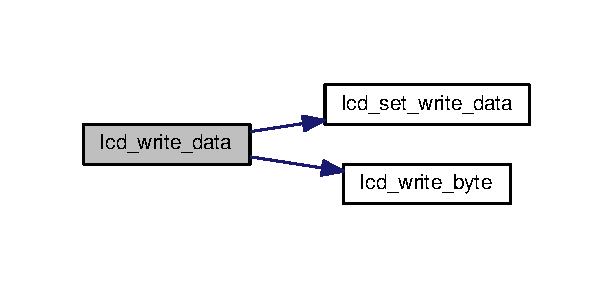
\includegraphics[width=294pt]{lcd8bit_8c_a082c749307f206b15a9cbeb775b03b5c_cgraph}
\end{center}
\end{figure}


\hypertarget{lcd8bit_8c_a348a0350888f0a9bc01ed290423e2af8}{\index{lcd8bit.\-c@{lcd8bit.\-c}!lcd\-\_\-write\-\_\-string@{lcd\-\_\-write\-\_\-string}}
\index{lcd\-\_\-write\-\_\-string@{lcd\-\_\-write\-\_\-string}!lcd8bit.c@{lcd8bit.\-c}}
\subsubsection[{lcd\-\_\-write\-\_\-string}]{\setlength{\rightskip}{0pt plus 5cm}void lcd\-\_\-write\-\_\-string (
\begin{DoxyParamCaption}
\item[{char $\ast$}]{x, }
\item[{uint8\-\_\-t}]{len}
\end{DoxyParamCaption}
)}}\label{lcd8bit_8c_a348a0350888f0a9bc01ed290423e2af8}


References lcd\-\_\-write\-\_\-data().



Here is the call graph for this function\-:
\nopagebreak
\begin{figure}[H]
\begin{center}
\leavevmode
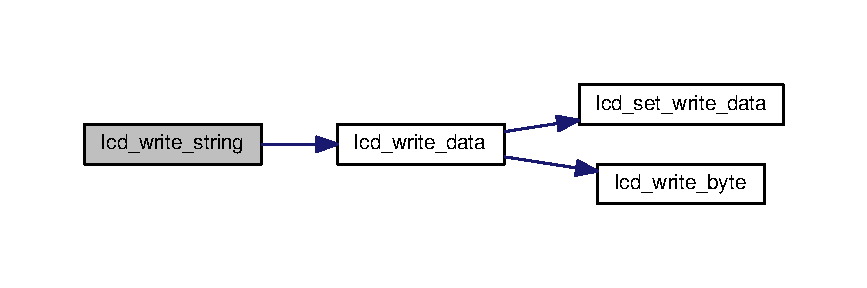
\includegraphics[width=350pt]{lcd8bit_8c_a348a0350888f0a9bc01ed290423e2af8_cgraph}
\end{center}
\end{figure}


\hypertarget{lcd8bit_8c_a9aa8378a804ddb51f770bd01665df653}{\index{lcd8bit.\-c@{lcd8bit.\-c}!lcd\-\_\-write\-\_\-string\-\_\-0@{lcd\-\_\-write\-\_\-string\-\_\-0}}
\index{lcd\-\_\-write\-\_\-string\-\_\-0@{lcd\-\_\-write\-\_\-string\-\_\-0}!lcd8bit.c@{lcd8bit.\-c}}
\subsubsection[{lcd\-\_\-write\-\_\-string\-\_\-0}]{\setlength{\rightskip}{0pt plus 5cm}void lcd\-\_\-write\-\_\-string\-\_\-0 (
\begin{DoxyParamCaption}
\item[{char $\ast$}]{x}
\end{DoxyParamCaption}
)}}\label{lcd8bit_8c_a9aa8378a804ddb51f770bd01665df653}


References lcd\-\_\-write\-\_\-data().



Referenced by die(), and main().



Here is the call graph for this function\-:
\nopagebreak
\begin{figure}[H]
\begin{center}
\leavevmode
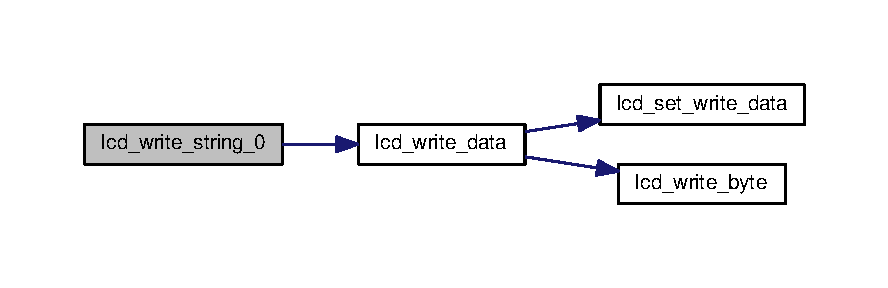
\includegraphics[width=350pt]{lcd8bit_8c_a9aa8378a804ddb51f770bd01665df653_cgraph}
\end{center}
\end{figure}


\hypertarget{lcd8bit_8c_a39cdfea82914e968ea1dbf7a8c6c9f9e}{\index{lcd8bit.\-c@{lcd8bit.\-c}!lcd\-\_\-write\-\_\-string\-\_\-p@{lcd\-\_\-write\-\_\-string\-\_\-p}}
\index{lcd\-\_\-write\-\_\-string\-\_\-p@{lcd\-\_\-write\-\_\-string\-\_\-p}!lcd8bit.c@{lcd8bit.\-c}}
\subsubsection[{lcd\-\_\-write\-\_\-string\-\_\-p}]{\setlength{\rightskip}{0pt plus 5cm}void lcd\-\_\-write\-\_\-string\-\_\-p (
\begin{DoxyParamCaption}
\item[{const char $\ast$}]{s}
\end{DoxyParamCaption}
)}}\label{lcd8bit_8c_a39cdfea82914e968ea1dbf7a8c6c9f9e}


References lcd\-\_\-write\-\_\-data().



Here is the call graph for this function\-:
\nopagebreak
\begin{figure}[H]
\begin{center}
\leavevmode
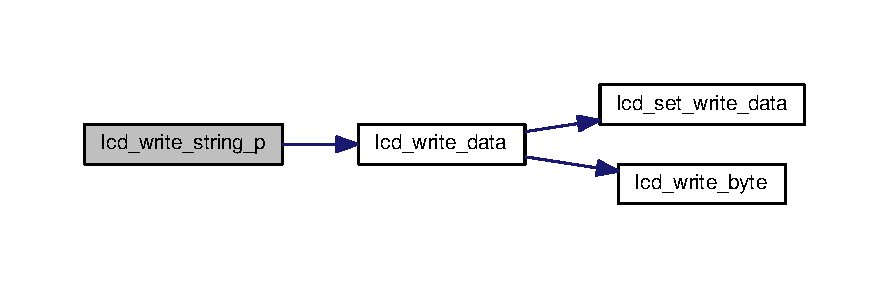
\includegraphics[width=350pt]{lcd8bit_8c_a39cdfea82914e968ea1dbf7a8c6c9f9e_cgraph}
\end{center}
\end{figure}



\hypertarget{lcd8bit_8h}{\section{lcd8bit/lcd8bit.h File Reference}
\label{lcd8bit_8h}\index{lcd8bit/lcd8bit.\-h@{lcd8bit/lcd8bit.\-h}}
}
This graph shows which files directly or indirectly include this file\-:\nopagebreak
\begin{figure}[H]
\begin{center}
\leavevmode
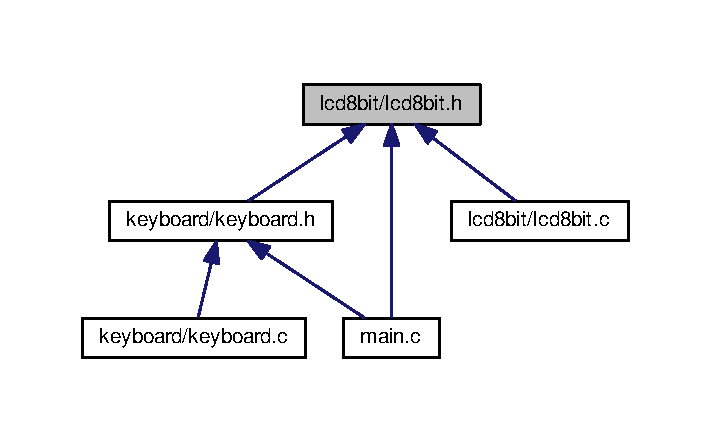
\includegraphics[width=341pt]{lcd8bit_8h__dep__incl}
\end{center}
\end{figure}
\subsection*{Functions}
\begin{DoxyCompactItemize}
\item 
void \hyperlink{lcd8bit_8h_a9d0f278e2fa5d8921d3a4fdd508a561e}{lcd\-\_\-set\-\_\-write\-\_\-instruction} ()
\item 
void \hyperlink{lcd8bit_8h_ad55e5c04e2a5354bfd4840be5e0eb5d1}{lcd\-\_\-set\-\_\-write\-\_\-data} ()
\item 
void \hyperlink{lcd8bit_8h_aef7fba4025d73ad60e375357e557bca3}{lcd\-\_\-write\-\_\-byte} (char c)
\item 
void \hyperlink{lcd8bit_8h_a88fdc90276b48773630acfc4525ff0db}{lcd\-\_\-clear\-\_\-and\-\_\-home} ()
\item 
void \hyperlink{lcd8bit_8h_a60675105b93bba6762aaab88d732365a}{lcd\-\_\-home} ()
\item 
void \hyperlink{lcd8bit_8h_affc4cf9b640d7c72fcb1e8be36c0183c}{lcd\-\_\-goto} (uint8\-\_\-t line, uint8\-\_\-t pos)
\item 
void \hyperlink{lcd8bit_8h_a8752d4e091188fcb07bbc9ae3c496e95}{lcd\-\_\-line\-\_\-one} ()
\item 
void \hyperlink{lcd8bit_8h_aa0b44a03031cc3639604de620e426021}{lcd\-\_\-line\-\_\-two} ()
\item 
void \hyperlink{lcd8bit_8h_a082c749307f206b15a9cbeb775b03b5c}{lcd\-\_\-write\-\_\-data} (char c)
\item 
void \hyperlink{lcd8bit_8h_a348a0350888f0a9bc01ed290423e2af8}{lcd\-\_\-write\-\_\-string} (char $\ast$x, uint8\-\_\-t len)
\item 
void \hyperlink{lcd8bit_8h_a9aa8378a804ddb51f770bd01665df653}{lcd\-\_\-write\-\_\-string\-\_\-0} (char $\ast$x)
\item 
void \hyperlink{lcd8bit_8h_a39cdfea82914e968ea1dbf7a8c6c9f9e}{lcd\-\_\-write\-\_\-string\-\_\-p} (const char $\ast$s)
\item 
void \hyperlink{lcd8bit_8h_ac23e73124dc9fabae95671fe71d074a6}{lcd\-\_\-init} ()
\end{DoxyCompactItemize}


\subsection{Function Documentation}
\hypertarget{lcd8bit_8h_a88fdc90276b48773630acfc4525ff0db}{\index{lcd8bit.\-h@{lcd8bit.\-h}!lcd\-\_\-clear\-\_\-and\-\_\-home@{lcd\-\_\-clear\-\_\-and\-\_\-home}}
\index{lcd\-\_\-clear\-\_\-and\-\_\-home@{lcd\-\_\-clear\-\_\-and\-\_\-home}!lcd8bit.h@{lcd8bit.\-h}}
\subsubsection[{lcd\-\_\-clear\-\_\-and\-\_\-home}]{\setlength{\rightskip}{0pt plus 5cm}void lcd\-\_\-clear\-\_\-and\-\_\-home (
\begin{DoxyParamCaption}
{}
\end{DoxyParamCaption}
)}}\label{lcd8bit_8h_a88fdc90276b48773630acfc4525ff0db}


References lcd\-\_\-set\-\_\-write\-\_\-instruction(), and lcd\-\_\-write\-\_\-byte().



Referenced by die(), lcd\-\_\-init(), and main().



Here is the call graph for this function\-:
\nopagebreak
\begin{figure}[H]
\begin{center}
\leavevmode
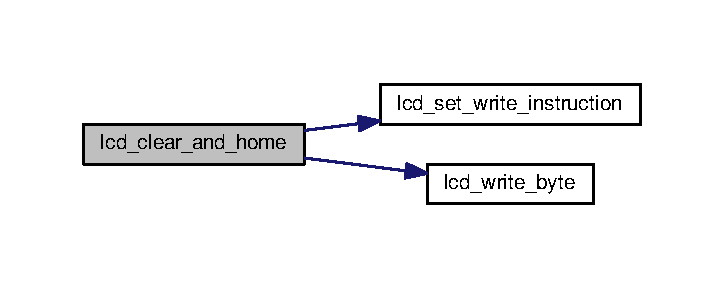
\includegraphics[width=348pt]{lcd8bit_8h_a88fdc90276b48773630acfc4525ff0db_cgraph}
\end{center}
\end{figure}


\hypertarget{lcd8bit_8h_affc4cf9b640d7c72fcb1e8be36c0183c}{\index{lcd8bit.\-h@{lcd8bit.\-h}!lcd\-\_\-goto@{lcd\-\_\-goto}}
\index{lcd\-\_\-goto@{lcd\-\_\-goto}!lcd8bit.h@{lcd8bit.\-h}}
\subsubsection[{lcd\-\_\-goto}]{\setlength{\rightskip}{0pt plus 5cm}void lcd\-\_\-goto (
\begin{DoxyParamCaption}
\item[{uint8\-\_\-t}]{line, }
\item[{uint8\-\_\-t}]{pos}
\end{DoxyParamCaption}
)}}\label{lcd8bit_8h_affc4cf9b640d7c72fcb1e8be36c0183c}


References lcd\-\_\-set\-\_\-write\-\_\-instruction(), and lcd\-\_\-write\-\_\-byte().



Referenced by lcd\-\_\-line\-\_\-one(), and lcd\-\_\-line\-\_\-two().



Here is the call graph for this function\-:
\nopagebreak
\begin{figure}[H]
\begin{center}
\leavevmode
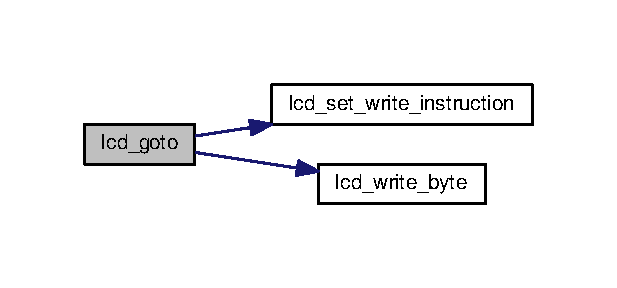
\includegraphics[width=296pt]{lcd8bit_8h_affc4cf9b640d7c72fcb1e8be36c0183c_cgraph}
\end{center}
\end{figure}


\hypertarget{lcd8bit_8h_a60675105b93bba6762aaab88d732365a}{\index{lcd8bit.\-h@{lcd8bit.\-h}!lcd\-\_\-home@{lcd\-\_\-home}}
\index{lcd\-\_\-home@{lcd\-\_\-home}!lcd8bit.h@{lcd8bit.\-h}}
\subsubsection[{lcd\-\_\-home}]{\setlength{\rightskip}{0pt plus 5cm}void lcd\-\_\-home (
\begin{DoxyParamCaption}
{}
\end{DoxyParamCaption}
)}}\label{lcd8bit_8h_a60675105b93bba6762aaab88d732365a}


References lcd\-\_\-set\-\_\-write\-\_\-instruction(), and lcd\-\_\-write\-\_\-byte().



Here is the call graph for this function\-:
\nopagebreak
\begin{figure}[H]
\begin{center}
\leavevmode
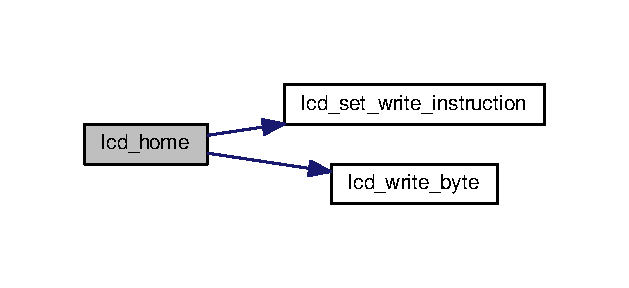
\includegraphics[width=302pt]{lcd8bit_8h_a60675105b93bba6762aaab88d732365a_cgraph}
\end{center}
\end{figure}


\hypertarget{lcd8bit_8h_ac23e73124dc9fabae95671fe71d074a6}{\index{lcd8bit.\-h@{lcd8bit.\-h}!lcd\-\_\-init@{lcd\-\_\-init}}
\index{lcd\-\_\-init@{lcd\-\_\-init}!lcd8bit.h@{lcd8bit.\-h}}
\subsubsection[{lcd\-\_\-init}]{\setlength{\rightskip}{0pt plus 5cm}void lcd\-\_\-init (
\begin{DoxyParamCaption}
{}
\end{DoxyParamCaption}
)}}\label{lcd8bit_8h_ac23e73124dc9fabae95671fe71d074a6}


References C\-O\-M\-M\-\_\-\-P\-O\-R\-T, D\-A\-T\-A\-\_\-\-P\-O\-R\-T, lcd\-\_\-clear\-\_\-and\-\_\-home(), L\-C\-D\-\_\-\-E, L\-C\-D\-\_\-\-R\-S, and lcd\-\_\-write\-\_\-byte().



Referenced by main().



Here is the call graph for this function\-:
\nopagebreak
\begin{figure}[H]
\begin{center}
\leavevmode
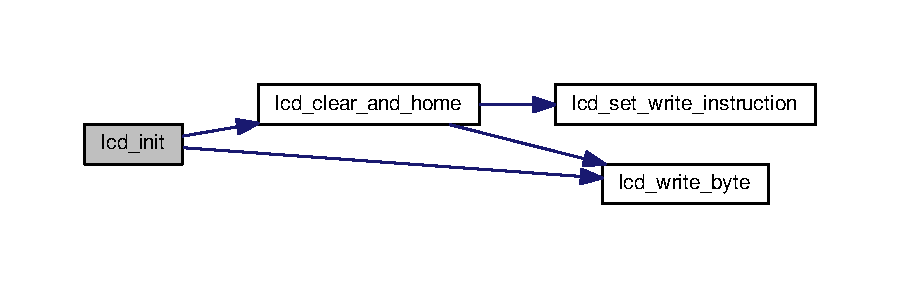
\includegraphics[width=350pt]{lcd8bit_8h_ac23e73124dc9fabae95671fe71d074a6_cgraph}
\end{center}
\end{figure}


\hypertarget{lcd8bit_8h_a8752d4e091188fcb07bbc9ae3c496e95}{\index{lcd8bit.\-h@{lcd8bit.\-h}!lcd\-\_\-line\-\_\-one@{lcd\-\_\-line\-\_\-one}}
\index{lcd\-\_\-line\-\_\-one@{lcd\-\_\-line\-\_\-one}!lcd8bit.h@{lcd8bit.\-h}}
\subsubsection[{lcd\-\_\-line\-\_\-one}]{\setlength{\rightskip}{0pt plus 5cm}void lcd\-\_\-line\-\_\-one (
\begin{DoxyParamCaption}
{}
\end{DoxyParamCaption}
)}}\label{lcd8bit_8h_a8752d4e091188fcb07bbc9ae3c496e95}


References lcd\-\_\-goto().



Referenced by die(), and main().



Here is the call graph for this function\-:
\nopagebreak
\begin{figure}[H]
\begin{center}
\leavevmode
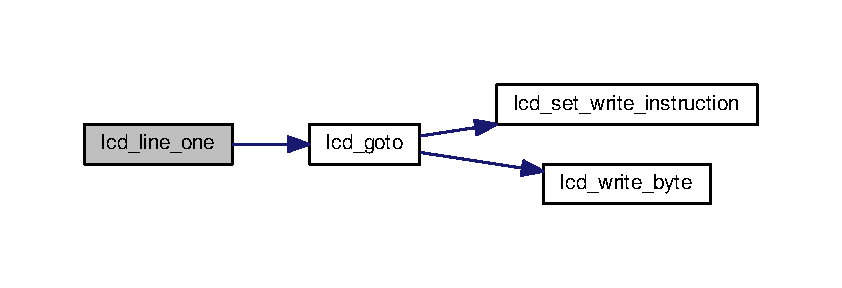
\includegraphics[width=350pt]{lcd8bit_8h_a8752d4e091188fcb07bbc9ae3c496e95_cgraph}
\end{center}
\end{figure}


\hypertarget{lcd8bit_8h_aa0b44a03031cc3639604de620e426021}{\index{lcd8bit.\-h@{lcd8bit.\-h}!lcd\-\_\-line\-\_\-two@{lcd\-\_\-line\-\_\-two}}
\index{lcd\-\_\-line\-\_\-two@{lcd\-\_\-line\-\_\-two}!lcd8bit.h@{lcd8bit.\-h}}
\subsubsection[{lcd\-\_\-line\-\_\-two}]{\setlength{\rightskip}{0pt plus 5cm}void lcd\-\_\-line\-\_\-two (
\begin{DoxyParamCaption}
{}
\end{DoxyParamCaption}
)}}\label{lcd8bit_8h_aa0b44a03031cc3639604de620e426021}


References lcd\-\_\-goto().



Referenced by die(), and main().



Here is the call graph for this function\-:
\nopagebreak
\begin{figure}[H]
\begin{center}
\leavevmode
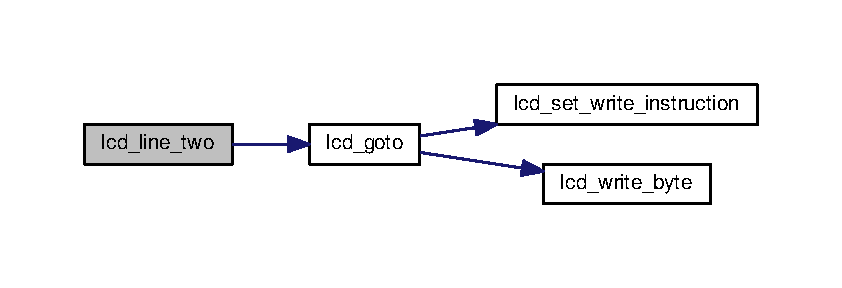
\includegraphics[width=350pt]{lcd8bit_8h_aa0b44a03031cc3639604de620e426021_cgraph}
\end{center}
\end{figure}


\hypertarget{lcd8bit_8h_ad55e5c04e2a5354bfd4840be5e0eb5d1}{\index{lcd8bit.\-h@{lcd8bit.\-h}!lcd\-\_\-set\-\_\-write\-\_\-data@{lcd\-\_\-set\-\_\-write\-\_\-data}}
\index{lcd\-\_\-set\-\_\-write\-\_\-data@{lcd\-\_\-set\-\_\-write\-\_\-data}!lcd8bit.h@{lcd8bit.\-h}}
\subsubsection[{lcd\-\_\-set\-\_\-write\-\_\-data}]{\setlength{\rightskip}{0pt plus 5cm}void lcd\-\_\-set\-\_\-write\-\_\-data (
\begin{DoxyParamCaption}
{}
\end{DoxyParamCaption}
)}}\label{lcd8bit_8h_ad55e5c04e2a5354bfd4840be5e0eb5d1}


References C\-O\-M\-M\-\_\-\-P\-O\-R\-T, and L\-C\-D\-\_\-\-R\-S.



Referenced by lcd\-\_\-write\-\_\-data().

\hypertarget{lcd8bit_8h_a9d0f278e2fa5d8921d3a4fdd508a561e}{\index{lcd8bit.\-h@{lcd8bit.\-h}!lcd\-\_\-set\-\_\-write\-\_\-instruction@{lcd\-\_\-set\-\_\-write\-\_\-instruction}}
\index{lcd\-\_\-set\-\_\-write\-\_\-instruction@{lcd\-\_\-set\-\_\-write\-\_\-instruction}!lcd8bit.h@{lcd8bit.\-h}}
\subsubsection[{lcd\-\_\-set\-\_\-write\-\_\-instruction}]{\setlength{\rightskip}{0pt plus 5cm}void lcd\-\_\-set\-\_\-write\-\_\-instruction (
\begin{DoxyParamCaption}
{}
\end{DoxyParamCaption}
)}}\label{lcd8bit_8h_a9d0f278e2fa5d8921d3a4fdd508a561e}


References C\-O\-M\-M\-\_\-\-P\-O\-R\-T, and L\-C\-D\-\_\-\-R\-S.



Referenced by lcd\-\_\-clear\-\_\-and\-\_\-home(), lcd\-\_\-goto(), and lcd\-\_\-home().

\hypertarget{lcd8bit_8h_aef7fba4025d73ad60e375357e557bca3}{\index{lcd8bit.\-h@{lcd8bit.\-h}!lcd\-\_\-write\-\_\-byte@{lcd\-\_\-write\-\_\-byte}}
\index{lcd\-\_\-write\-\_\-byte@{lcd\-\_\-write\-\_\-byte}!lcd8bit.h@{lcd8bit.\-h}}
\subsubsection[{lcd\-\_\-write\-\_\-byte}]{\setlength{\rightskip}{0pt plus 5cm}void lcd\-\_\-write\-\_\-byte (
\begin{DoxyParamCaption}
\item[{char}]{c}
\end{DoxyParamCaption}
)}}\label{lcd8bit_8h_aef7fba4025d73ad60e375357e557bca3}


References C\-O\-M\-M\-\_\-\-P\-O\-R\-T, D\-A\-T\-A\-\_\-\-P\-O\-R\-T, and L\-C\-D\-\_\-\-E.



Referenced by lcd\-\_\-clear\-\_\-and\-\_\-home(), lcd\-\_\-goto(), lcd\-\_\-home(), lcd\-\_\-init(), and lcd\-\_\-write\-\_\-data().

\hypertarget{lcd8bit_8h_a082c749307f206b15a9cbeb775b03b5c}{\index{lcd8bit.\-h@{lcd8bit.\-h}!lcd\-\_\-write\-\_\-data@{lcd\-\_\-write\-\_\-data}}
\index{lcd\-\_\-write\-\_\-data@{lcd\-\_\-write\-\_\-data}!lcd8bit.h@{lcd8bit.\-h}}
\subsubsection[{lcd\-\_\-write\-\_\-data}]{\setlength{\rightskip}{0pt plus 5cm}void lcd\-\_\-write\-\_\-data (
\begin{DoxyParamCaption}
\item[{char}]{c}
\end{DoxyParamCaption}
)}}\label{lcd8bit_8h_a082c749307f206b15a9cbeb775b03b5c}


References lcd\-\_\-set\-\_\-write\-\_\-data(), and lcd\-\_\-write\-\_\-byte().



Referenced by lcd\-\_\-write\-\_\-string(), lcd\-\_\-write\-\_\-string\-\_\-0(), and lcd\-\_\-write\-\_\-string\-\_\-p().



Here is the call graph for this function\-:
\nopagebreak
\begin{figure}[H]
\begin{center}
\leavevmode
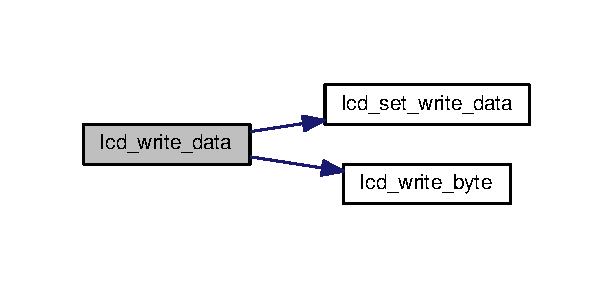
\includegraphics[width=294pt]{lcd8bit_8h_a082c749307f206b15a9cbeb775b03b5c_cgraph}
\end{center}
\end{figure}


\hypertarget{lcd8bit_8h_a348a0350888f0a9bc01ed290423e2af8}{\index{lcd8bit.\-h@{lcd8bit.\-h}!lcd\-\_\-write\-\_\-string@{lcd\-\_\-write\-\_\-string}}
\index{lcd\-\_\-write\-\_\-string@{lcd\-\_\-write\-\_\-string}!lcd8bit.h@{lcd8bit.\-h}}
\subsubsection[{lcd\-\_\-write\-\_\-string}]{\setlength{\rightskip}{0pt plus 5cm}void lcd\-\_\-write\-\_\-string (
\begin{DoxyParamCaption}
\item[{char $\ast$}]{x, }
\item[{uint8\-\_\-t}]{len}
\end{DoxyParamCaption}
)}}\label{lcd8bit_8h_a348a0350888f0a9bc01ed290423e2af8}


References lcd\-\_\-write\-\_\-data().



Here is the call graph for this function\-:
\nopagebreak
\begin{figure}[H]
\begin{center}
\leavevmode
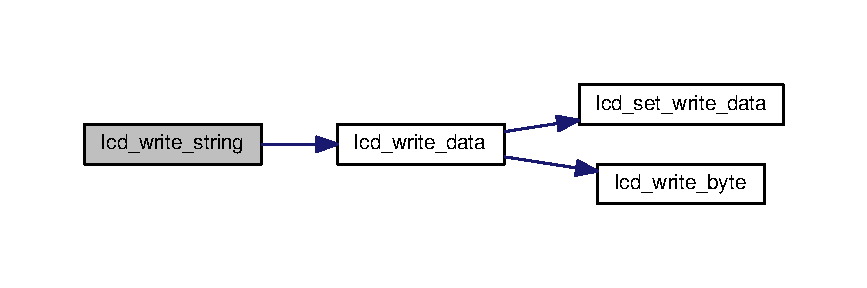
\includegraphics[width=350pt]{lcd8bit_8h_a348a0350888f0a9bc01ed290423e2af8_cgraph}
\end{center}
\end{figure}


\hypertarget{lcd8bit_8h_a9aa8378a804ddb51f770bd01665df653}{\index{lcd8bit.\-h@{lcd8bit.\-h}!lcd\-\_\-write\-\_\-string\-\_\-0@{lcd\-\_\-write\-\_\-string\-\_\-0}}
\index{lcd\-\_\-write\-\_\-string\-\_\-0@{lcd\-\_\-write\-\_\-string\-\_\-0}!lcd8bit.h@{lcd8bit.\-h}}
\subsubsection[{lcd\-\_\-write\-\_\-string\-\_\-0}]{\setlength{\rightskip}{0pt plus 5cm}void lcd\-\_\-write\-\_\-string\-\_\-0 (
\begin{DoxyParamCaption}
\item[{char $\ast$}]{x}
\end{DoxyParamCaption}
)}}\label{lcd8bit_8h_a9aa8378a804ddb51f770bd01665df653}


References lcd\-\_\-write\-\_\-data().



Referenced by die(), and main().



Here is the call graph for this function\-:
\nopagebreak
\begin{figure}[H]
\begin{center}
\leavevmode
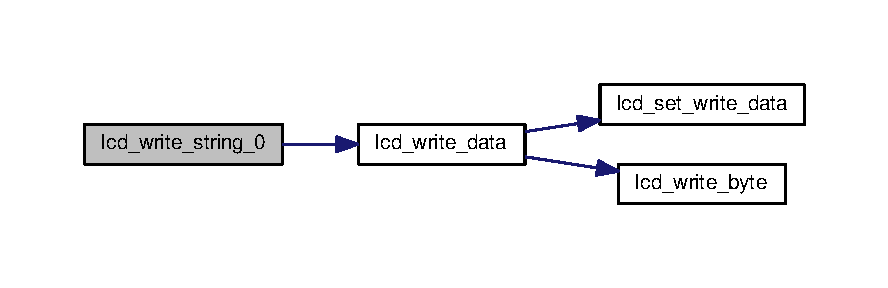
\includegraphics[width=350pt]{lcd8bit_8h_a9aa8378a804ddb51f770bd01665df653_cgraph}
\end{center}
\end{figure}


\hypertarget{lcd8bit_8h_a39cdfea82914e968ea1dbf7a8c6c9f9e}{\index{lcd8bit.\-h@{lcd8bit.\-h}!lcd\-\_\-write\-\_\-string\-\_\-p@{lcd\-\_\-write\-\_\-string\-\_\-p}}
\index{lcd\-\_\-write\-\_\-string\-\_\-p@{lcd\-\_\-write\-\_\-string\-\_\-p}!lcd8bit.h@{lcd8bit.\-h}}
\subsubsection[{lcd\-\_\-write\-\_\-string\-\_\-p}]{\setlength{\rightskip}{0pt plus 5cm}void lcd\-\_\-write\-\_\-string\-\_\-p (
\begin{DoxyParamCaption}
\item[{const char $\ast$}]{s}
\end{DoxyParamCaption}
)}}\label{lcd8bit_8h_a39cdfea82914e968ea1dbf7a8c6c9f9e}


References lcd\-\_\-write\-\_\-data().



Here is the call graph for this function\-:
\nopagebreak
\begin{figure}[H]
\begin{center}
\leavevmode
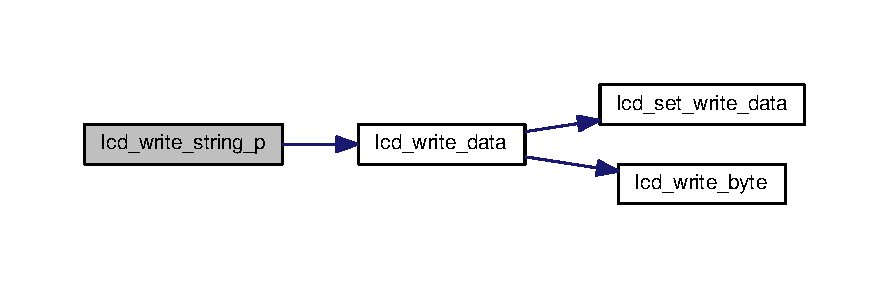
\includegraphics[width=350pt]{lcd8bit_8h_a39cdfea82914e968ea1dbf7a8c6c9f9e_cgraph}
\end{center}
\end{figure}



\hypertarget{list_8c}{\section{list/list.c File Reference}
\label{list_8c}\index{list/list.\-c@{list/list.\-c}}
}
{\ttfamily \#include $<$stdlib.\-h$>$}\\*
{\ttfamily \#include $<$stdio.\-h$>$}\\*
{\ttfamily \#include $<$string.\-h$>$}\\*
{\ttfamily \#include \char`\"{}list.\-h\char`\"{}}\\*
Include dependency graph for list.\-c\-:\nopagebreak
\begin{figure}[H]
\begin{center}
\leavevmode
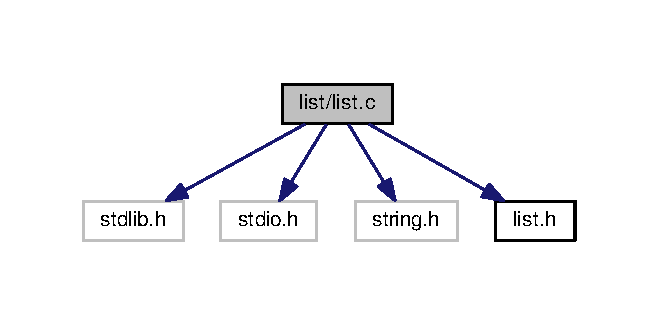
\includegraphics[width=316pt]{list_8c__incl}
\end{center}
\end{figure}
\subsection*{Functions}
\begin{DoxyCompactItemize}
\item 
struct \hyperlink{structonode}{onode} $\ast$ \hyperlink{list_8c_ace16262cb905d559225fe768d32d574b}{new\-Node} (struct \hyperlink{structorder}{order} $\ast$data)
\begin{DoxyCompactList}\small\item\em Returns a new linked list node filled in with the given order. \end{DoxyCompactList}\item 
struct \hyperlink{structonode}{onode} $\ast$ \hyperlink{list_8c_ad0b81dec75f1c7bfca0ec9a6f9ae2f30}{new\-Node\-By\-Ref} (struct \hyperlink{structorder}{order} $\ast$data)
\begin{DoxyCompactList}\small\item\em Returns a new linked list node filled in with the given order. \end{DoxyCompactList}\item 
void \hyperlink{list_8c_ab20a8a7735339bdced34d2d97304b583}{push\-Node} (struct \hyperlink{structonode}{onode} $\ast$$\ast$head, struct \hyperlink{structonode}{onode} $\ast$node)
\begin{DoxyCompactList}\small\item\em In a linked list with $\ast$head as the head pointer, adds the given node to the front of the list. \end{DoxyCompactList}\item 
void \hyperlink{list_8c_a68123d7e3ab7016228af42c9ae480626}{sort} (struct \hyperlink{structonode}{onode} $\ast$$\ast$head)
\begin{DoxyCompactList}\small\item\em Performes insertion sort on the list by comparing the Order\-I\-D. \end{DoxyCompactList}\item 
void \hyperlink{list_8c_a48838b111c5cba7f2503e6cb34992371}{swap} (struct \hyperlink{structonode}{onode} $\ast$$\ast$head, struct \hyperlink{structonode}{onode} $\ast$node1, struct \hyperlink{structonode}{onode} $\ast$node2)
\item 
void \hyperlink{list_8c_aac2759a1682242fc31ec173316a40647}{insert\-Node} (struct \hyperlink{structonode}{onode} $\ast$$\ast$head, struct \hyperlink{structonode}{onode} $\ast$prev\-Node, struct \hyperlink{structonode}{onode} $\ast$inserting\-Node)
\begin{DoxyCompactList}\small\item\em Insert the given node after the prev\-Node. \end{DoxyCompactList}\item 
void \hyperlink{list_8c_a57726dc16efcab2ebe228494fce04bf0}{evict\-Node} (struct \hyperlink{structonode}{onode} $\ast$$\ast$head, struct \hyperlink{structonode}{onode} $\ast$node)
\begin{DoxyCompactList}\small\item\em Internally removes the specified node from the list, and updates the linked list. \end{DoxyCompactList}\item 
void \hyperlink{list_8c_a440d2fb8a7f4399ae63fadcd19e67353}{delete\-Node\-Only} (struct \hyperlink{structonode}{onode} $\ast$$\ast$head, struct \hyperlink{structonode}{onode} $\ast$node)
\begin{DoxyCompactList}\small\item\em Removes the specified node from the list, and does N\-O\-T free memory the node is using. \end{DoxyCompactList}\item 
void \hyperlink{list_8c_a59bce7be7525819723563c7a5d83065f}{delete\-Node} (struct \hyperlink{structonode}{onode} $\ast$$\ast$head, struct \hyperlink{structonode}{onode} $\ast$node)
\begin{DoxyCompactList}\small\item\em Removes the specified node from the list, and frees all memory the node is using. \end{DoxyCompactList}\item 
void \hyperlink{list_8c_ac334adb29fda2c483930f77a871bc049}{print\-List} (struct \hyperlink{structonode}{onode} $\ast$node, void($\ast$print\-Item)(struct \hyperlink{structorder}{order} $\ast$, F\-I\-L\-E $\ast$), F\-I\-L\-E $\ast$out)
\item 
struct \hyperlink{structonode}{onode} $\ast$ \hyperlink{list_8c_ace9faaeb801bbdf650d93f4a8b075c4c}{get\-Next\-Order} (struct \hyperlink{structonode}{onode} $\ast$order\-\_\-node)
\begin{DoxyCompactList}\small\item\em Simply returns the next node in the list, or N\-U\-L\-L if there are no further nodes. \end{DoxyCompactList}\item 
struct \hyperlink{structonode}{onode} $\ast$ \hyperlink{list_8c_a9960b22010f913d546f29222e8fe71c1}{get\-Prev\-Order} (struct \hyperlink{structonode}{onode} $\ast$order\-\_\-node)
\item 
struct \hyperlink{structorder}{order} $\ast$ \hyperlink{list_8c_a926f037e453969ff428e61cf5d0300ac}{get\-Order\-Data} (struct \hyperlink{structonode}{onode} $\ast$order\-\_\-node)
\item 
int \hyperlink{list_8c_a2eecdd9441c2808156e2823cf2647acf}{get\-Order\-Id} (struct \hyperlink{structorder}{order} $\ast$order\-Data)
\item 
char \hyperlink{list_8c_a73e537f55ebe8a58816876e8c62c0613}{get\-Order\-Startstop} (struct \hyperlink{structorder}{order} $\ast$order\-Data, char bank\-Num)
\item 
int \hyperlink{list_8c_a2300cf7be3777ca0d27069a65378d41d}{get\-Order\-Note} (struct \hyperlink{structorder}{order} $\ast$order\-Data, char bank\-Num)
\item 
void \hyperlink{list_8c_a2772e75f849e208065637fb8e40816f6}{set\-Order\-Startstop} (struct \hyperlink{structorder}{order} $\ast$order\-Data, char new\-Startstop, char bank\-Num)
\item 
void \hyperlink{list_8c_ac4be440700d9a5aba95aab1486c043d6}{set\-Order\-Note} (struct \hyperlink{structorder}{order} $\ast$order\-Data, char new\-Note, char bank\-Num)
\item 
void \hyperlink{list_8c_aa1c09c554716a9c9267e6bdea34f4040}{set\-Order\-Id} (struct \hyperlink{structorder}{order} $\ast$order\-Data, int id)
\item 
void \hyperlink{list_8c_afd387a5ae038d1e69411b6e5dee52bfe}{delete\-List} (struct \hyperlink{structonode}{onode} $\ast$$\ast$head)
\begin{DoxyCompactList}\small\item\em Deletes every node in the list with $\ast$head as the head pointer. \end{DoxyCompactList}\item 
void \hyperlink{list_8c_a1ca006182933095d94eb455540ff162d}{delete\-Just\-List} (struct \hyperlink{structonode}{onode} $\ast$$\ast$head)
\begin{DoxyCompactList}\small\item\em Deletes every node E\-X\-C\-E\-P\-T the head in the list with $\ast$head as the head pointer. \end{DoxyCompactList}\end{DoxyCompactItemize}
\begin{Indent}{\bf group1 Content Management\-: Setters and Getters for linked\-List}\par
{\em Setters and Getters for linked\-List }\begin{DoxyCompactItemize}
\item 
struct \hyperlink{structonode}{onode} $\ast$ \hyperlink{list_8c_a495419524f4f52b77b4734361093ee47}{get\-Order\-Node} (struct \hyperlink{structonode}{onode} $\ast$head, int id)
\begin{DoxyCompactList}\small\item\em Returns the pointer to the node containing the given word in the linked list with head as the head pointer. \end{DoxyCompactList}\end{DoxyCompactItemize}
\end{Indent}
\subsection*{Variables}
\begin{DoxyCompactItemize}
\item 
int \hyperlink{list_8c_a71867e609034d4dbd6d0ad8d84540e59}{g} =0
\end{DoxyCompactItemize}


\subsection{Function Documentation}
\hypertarget{list_8c_a1ca006182933095d94eb455540ff162d}{\index{list.\-c@{list.\-c}!delete\-Just\-List@{delete\-Just\-List}}
\index{delete\-Just\-List@{delete\-Just\-List}!list.c@{list.\-c}}
\subsubsection[{delete\-Just\-List}]{\setlength{\rightskip}{0pt plus 5cm}void delete\-Just\-List (
\begin{DoxyParamCaption}
\item[{struct {\bf onode} $\ast$$\ast$}]{head}
\end{DoxyParamCaption}
)}}\label{list_8c_a1ca006182933095d94eb455540ff162d}


Deletes every node E\-X\-C\-E\-P\-T the head in the list with $\ast$head as the head pointer. 

After calling this function, all memory used by the list should be freed, and $\ast$head should be N\-U\-L\-L. 

References onode\-::next.

\hypertarget{list_8c_afd387a5ae038d1e69411b6e5dee52bfe}{\index{list.\-c@{list.\-c}!delete\-List@{delete\-List}}
\index{delete\-List@{delete\-List}!list.c@{list.\-c}}
\subsubsection[{delete\-List}]{\setlength{\rightskip}{0pt plus 5cm}void delete\-List (
\begin{DoxyParamCaption}
\item[{struct {\bf onode} $\ast$$\ast$}]{head}
\end{DoxyParamCaption}
)}}\label{list_8c_afd387a5ae038d1e69411b6e5dee52bfe}


Deletes every node in the list with $\ast$head as the head pointer. 

After calling this function, all memory used by the list should be freed, and $\ast$head should be N\-U\-L\-L. 

References onode\-::data, and onode\-::next.

\hypertarget{list_8c_a59bce7be7525819723563c7a5d83065f}{\index{list.\-c@{list.\-c}!delete\-Node@{delete\-Node}}
\index{delete\-Node@{delete\-Node}!list.c@{list.\-c}}
\subsubsection[{delete\-Node}]{\setlength{\rightskip}{0pt plus 5cm}void delete\-Node (
\begin{DoxyParamCaption}
\item[{struct {\bf onode} $\ast$$\ast$}]{head, }
\item[{struct {\bf onode} $\ast$}]{node}
\end{DoxyParamCaption}
)}}\label{list_8c_a59bce7be7525819723563c7a5d83065f}


Removes the specified node from the list, and frees all memory the node is using. 

Remember if $\ast$head is the node being deleted, it must be updated. 

References onode\-::data, and delete\-Node\-Only().



Here is the call graph for this function\-:
\nopagebreak
\begin{figure}[H]
\begin{center}
\leavevmode
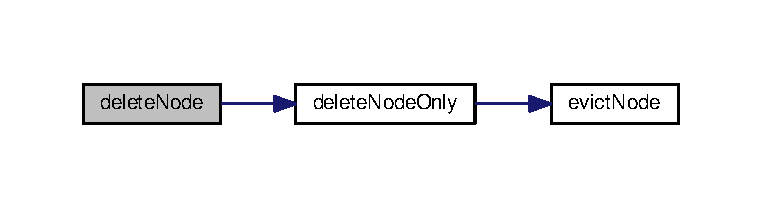
\includegraphics[width=350pt]{list_8c_a59bce7be7525819723563c7a5d83065f_cgraph}
\end{center}
\end{figure}


\hypertarget{list_8c_a440d2fb8a7f4399ae63fadcd19e67353}{\index{list.\-c@{list.\-c}!delete\-Node\-Only@{delete\-Node\-Only}}
\index{delete\-Node\-Only@{delete\-Node\-Only}!list.c@{list.\-c}}
\subsubsection[{delete\-Node\-Only}]{\setlength{\rightskip}{0pt plus 5cm}void delete\-Node\-Only (
\begin{DoxyParamCaption}
\item[{struct {\bf onode} $\ast$$\ast$}]{head, }
\item[{struct {\bf onode} $\ast$}]{node}
\end{DoxyParamCaption}
)}}\label{list_8c_a440d2fb8a7f4399ae63fadcd19e67353}


Removes the specified node from the list, and does N\-O\-T free memory the node is using. 

Remember if $\ast$head is the node being deleted, it must be updated. 

References evict\-Node().



Referenced by delete\-Node().



Here is the call graph for this function\-:
\nopagebreak
\begin{figure}[H]
\begin{center}
\leavevmode
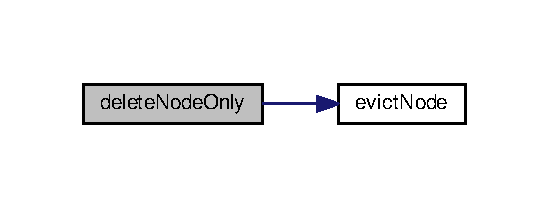
\includegraphics[width=264pt]{list_8c_a440d2fb8a7f4399ae63fadcd19e67353_cgraph}
\end{center}
\end{figure}


\hypertarget{list_8c_a57726dc16efcab2ebe228494fce04bf0}{\index{list.\-c@{list.\-c}!evict\-Node@{evict\-Node}}
\index{evict\-Node@{evict\-Node}!list.c@{list.\-c}}
\subsubsection[{evict\-Node}]{\setlength{\rightskip}{0pt plus 5cm}void evict\-Node (
\begin{DoxyParamCaption}
\item[{struct {\bf onode} $\ast$$\ast$}]{head, }
\item[{struct {\bf onode} $\ast$}]{node}
\end{DoxyParamCaption}
)}}\label{list_8c_a57726dc16efcab2ebe228494fce04bf0}


Internally removes the specified node from the list, and updates the linked list. 



References onode\-::next, and onode\-::prev.



Referenced by delete\-Node\-Only().

\hypertarget{list_8c_ace9faaeb801bbdf650d93f4a8b075c4c}{\index{list.\-c@{list.\-c}!get\-Next\-Order@{get\-Next\-Order}}
\index{get\-Next\-Order@{get\-Next\-Order}!list.c@{list.\-c}}
\subsubsection[{get\-Next\-Order}]{\setlength{\rightskip}{0pt plus 5cm}struct {\bf onode}$\ast$ get\-Next\-Order (
\begin{DoxyParamCaption}
\item[{struct {\bf onode} $\ast$}]{order\-\_\-node}
\end{DoxyParamCaption}
)}}\label{list_8c_ace9faaeb801bbdf650d93f4a8b075c4c}


Simply returns the next node in the list, or N\-U\-L\-L if there are no further nodes. 



References onode\-::next.



Referenced by sort().

\hypertarget{list_8c_a926f037e453969ff428e61cf5d0300ac}{\index{list.\-c@{list.\-c}!get\-Order\-Data@{get\-Order\-Data}}
\index{get\-Order\-Data@{get\-Order\-Data}!list.c@{list.\-c}}
\subsubsection[{get\-Order\-Data}]{\setlength{\rightskip}{0pt plus 5cm}struct {\bf order}$\ast$ get\-Order\-Data (
\begin{DoxyParamCaption}
\item[{struct {\bf onode} $\ast$}]{order\-\_\-node}
\end{DoxyParamCaption}
)}}\label{list_8c_a926f037e453969ff428e61cf5d0300ac}


References onode\-::data.

\hypertarget{list_8c_a2eecdd9441c2808156e2823cf2647acf}{\index{list.\-c@{list.\-c}!get\-Order\-Id@{get\-Order\-Id}}
\index{get\-Order\-Id@{get\-Order\-Id}!list.c@{list.\-c}}
\subsubsection[{get\-Order\-Id}]{\setlength{\rightskip}{0pt plus 5cm}int get\-Order\-Id (
\begin{DoxyParamCaption}
\item[{struct {\bf order} $\ast$}]{order\-Data}
\end{DoxyParamCaption}
)}}\label{list_8c_a2eecdd9441c2808156e2823cf2647acf}


References order\-::id.



Referenced by sort().

\hypertarget{list_8c_a495419524f4f52b77b4734361093ee47}{\index{list.\-c@{list.\-c}!get\-Order\-Node@{get\-Order\-Node}}
\index{get\-Order\-Node@{get\-Order\-Node}!list.c@{list.\-c}}
\subsubsection[{get\-Order\-Node}]{\setlength{\rightskip}{0pt plus 5cm}struct {\bf onode} $\ast$ get\-Order\-Node (
\begin{DoxyParamCaption}
\item[{struct {\bf onode} $\ast$}]{head, }
\item[{int}]{id}
\end{DoxyParamCaption}
)}}\label{list_8c_a495419524f4f52b77b4734361093ee47}


Returns the pointer to the node containing the given word in the linked list with head as the head pointer. 

In a linked list with $\ast$head as the head pointer, returns the onode with the given order id.

If a node with the given word cannot be found, the function returns N\-U\-L\-L. 

References onode\-::data, order\-::id, and onode\-::next.

\hypertarget{list_8c_a2300cf7be3777ca0d27069a65378d41d}{\index{list.\-c@{list.\-c}!get\-Order\-Note@{get\-Order\-Note}}
\index{get\-Order\-Note@{get\-Order\-Note}!list.c@{list.\-c}}
\subsubsection[{get\-Order\-Note}]{\setlength{\rightskip}{0pt plus 5cm}int get\-Order\-Note (
\begin{DoxyParamCaption}
\item[{struct {\bf order} $\ast$}]{order\-Data, }
\item[{char}]{bank\-Num}
\end{DoxyParamCaption}
)}}\label{list_8c_a2300cf7be3777ca0d27069a65378d41d}


References order\-::bank1\-\_\-note, order\-::bank2\-\_\-note, and order\-::bank3\-\_\-note.

\hypertarget{list_8c_a73e537f55ebe8a58816876e8c62c0613}{\index{list.\-c@{list.\-c}!get\-Order\-Startstop@{get\-Order\-Startstop}}
\index{get\-Order\-Startstop@{get\-Order\-Startstop}!list.c@{list.\-c}}
\subsubsection[{get\-Order\-Startstop}]{\setlength{\rightskip}{0pt plus 5cm}char get\-Order\-Startstop (
\begin{DoxyParamCaption}
\item[{struct {\bf order} $\ast$}]{order\-Data, }
\item[{char}]{bank\-Num}
\end{DoxyParamCaption}
)}}\label{list_8c_a73e537f55ebe8a58816876e8c62c0613}


References order\-::bank1\-\_\-startstop, order\-::bank2\-\_\-startstop, and order\-::bank3\-\_\-startstop.

\hypertarget{list_8c_a9960b22010f913d546f29222e8fe71c1}{\index{list.\-c@{list.\-c}!get\-Prev\-Order@{get\-Prev\-Order}}
\index{get\-Prev\-Order@{get\-Prev\-Order}!list.c@{list.\-c}}
\subsubsection[{get\-Prev\-Order}]{\setlength{\rightskip}{0pt plus 5cm}struct {\bf onode}$\ast$ get\-Prev\-Order (
\begin{DoxyParamCaption}
\item[{struct {\bf onode} $\ast$}]{order\-\_\-node}
\end{DoxyParamCaption}
)}}\label{list_8c_a9960b22010f913d546f29222e8fe71c1}


References onode\-::prev.



Referenced by sort().

\hypertarget{list_8c_aac2759a1682242fc31ec173316a40647}{\index{list.\-c@{list.\-c}!insert\-Node@{insert\-Node}}
\index{insert\-Node@{insert\-Node}!list.c@{list.\-c}}
\subsubsection[{insert\-Node}]{\setlength{\rightskip}{0pt plus 5cm}void insert\-Node (
\begin{DoxyParamCaption}
\item[{struct {\bf onode} $\ast$$\ast$}]{head, }
\item[{struct {\bf onode} $\ast$}]{prev\-Node, }
\item[{struct {\bf onode} $\ast$}]{inserting\-Node}
\end{DoxyParamCaption}
)}}\label{list_8c_aac2759a1682242fc31ec173316a40647}


Insert the given node after the prev\-Node. 

If the prev\-Node is N\-U\-L\-L, then the given node is inserted at the head of the list. 

References onode\-::next, onode\-::prev, and push\-Node().



Here is the call graph for this function\-:
\nopagebreak
\begin{figure}[H]
\begin{center}
\leavevmode
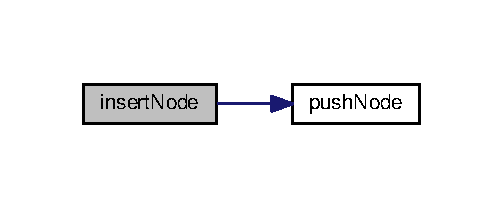
\includegraphics[width=242pt]{list_8c_aac2759a1682242fc31ec173316a40647_cgraph}
\end{center}
\end{figure}


\hypertarget{list_8c_ace16262cb905d559225fe768d32d574b}{\index{list.\-c@{list.\-c}!new\-Node@{new\-Node}}
\index{new\-Node@{new\-Node}!list.c@{list.\-c}}
\subsubsection[{new\-Node}]{\setlength{\rightskip}{0pt plus 5cm}struct {\bf onode}$\ast$ new\-Node (
\begin{DoxyParamCaption}
\item[{struct {\bf order} $\ast$}]{data}
\end{DoxyParamCaption}
)}}\label{list_8c_ace16262cb905d559225fe768d32d574b}


Returns a new linked list node filled in with the given order. 

Returns a new linked list node filled in with the given order, The function allocates a new order and copy the values stored in data then allocate a linked list node.

The order is copied into the node as a new instance. 

References order\-::bank1\-\_\-note, order\-::bank1\-\_\-startstop, order\-::bank2\-\_\-note, order\-::bank2\-\_\-startstop, order\-::bank3\-\_\-note, order\-::bank3\-\_\-startstop, g, and order\-::id.



Referenced by main().

\hypertarget{list_8c_ad0b81dec75f1c7bfca0ec9a6f9ae2f30}{\index{list.\-c@{list.\-c}!new\-Node\-By\-Ref@{new\-Node\-By\-Ref}}
\index{new\-Node\-By\-Ref@{new\-Node\-By\-Ref}!list.c@{list.\-c}}
\subsubsection[{new\-Node\-By\-Ref}]{\setlength{\rightskip}{0pt plus 5cm}struct {\bf onode}$\ast$ new\-Node\-By\-Ref (
\begin{DoxyParamCaption}
\item[{struct {\bf order} $\ast$}]{data}
\end{DoxyParamCaption}
)}}\label{list_8c_ad0b81dec75f1c7bfca0ec9a6f9ae2f30}


Returns a new linked list node filled in with the given order. 

Returns a new linked list node filled in with the given order, The function allocates a new order and copy the values stored in data then allocate a linked list node.

The order is inserted by reference. 

References onode\-::data.

\hypertarget{list_8c_ac334adb29fda2c483930f77a871bc049}{\index{list.\-c@{list.\-c}!print\-List@{print\-List}}
\index{print\-List@{print\-List}!list.c@{list.\-c}}
\subsubsection[{print\-List}]{\setlength{\rightskip}{0pt plus 5cm}void print\-List (
\begin{DoxyParamCaption}
\item[{struct {\bf onode} $\ast$}]{node, }
\item[{void($\ast$)(struct {\bf order} $\ast$, F\-I\-L\-E $\ast$)}]{print\-Item, }
\item[{F\-I\-L\-E $\ast$}]{out}
\end{DoxyParamCaption}
)}}\label{list_8c_ac334adb29fda2c483930f77a871bc049}


References onode\-::data, and onode\-::next.

\hypertarget{list_8c_ab20a8a7735339bdced34d2d97304b583}{\index{list.\-c@{list.\-c}!push\-Node@{push\-Node}}
\index{push\-Node@{push\-Node}!list.c@{list.\-c}}
\subsubsection[{push\-Node}]{\setlength{\rightskip}{0pt plus 5cm}void push\-Node (
\begin{DoxyParamCaption}
\item[{struct {\bf onode} $\ast$$\ast$}]{head, }
\item[{struct {\bf onode} $\ast$}]{node}
\end{DoxyParamCaption}
)}}\label{list_8c_ab20a8a7735339bdced34d2d97304b583}


In a linked list with $\ast$head as the head pointer, adds the given node to the front of the list. 



References onode\-::next, and onode\-::prev.



Referenced by insert\-Node(), and main().

\hypertarget{list_8c_aa1c09c554716a9c9267e6bdea34f4040}{\index{list.\-c@{list.\-c}!set\-Order\-Id@{set\-Order\-Id}}
\index{set\-Order\-Id@{set\-Order\-Id}!list.c@{list.\-c}}
\subsubsection[{set\-Order\-Id}]{\setlength{\rightskip}{0pt plus 5cm}void set\-Order\-Id (
\begin{DoxyParamCaption}
\item[{struct {\bf order} $\ast$}]{order\-Data, }
\item[{int}]{id}
\end{DoxyParamCaption}
)}}\label{list_8c_aa1c09c554716a9c9267e6bdea34f4040}


References order\-::id.

\hypertarget{list_8c_ac4be440700d9a5aba95aab1486c043d6}{\index{list.\-c@{list.\-c}!set\-Order\-Note@{set\-Order\-Note}}
\index{set\-Order\-Note@{set\-Order\-Note}!list.c@{list.\-c}}
\subsubsection[{set\-Order\-Note}]{\setlength{\rightskip}{0pt plus 5cm}void set\-Order\-Note (
\begin{DoxyParamCaption}
\item[{struct {\bf order} $\ast$}]{order\-Data, }
\item[{char}]{new\-Note, }
\item[{char}]{bank\-Num}
\end{DoxyParamCaption}
)}}\label{list_8c_ac4be440700d9a5aba95aab1486c043d6}


References order\-::bank1\-\_\-note, order\-::bank2\-\_\-note, and order\-::bank3\-\_\-note.

\hypertarget{list_8c_a2772e75f849e208065637fb8e40816f6}{\index{list.\-c@{list.\-c}!set\-Order\-Startstop@{set\-Order\-Startstop}}
\index{set\-Order\-Startstop@{set\-Order\-Startstop}!list.c@{list.\-c}}
\subsubsection[{set\-Order\-Startstop}]{\setlength{\rightskip}{0pt plus 5cm}void set\-Order\-Startstop (
\begin{DoxyParamCaption}
\item[{struct {\bf order} $\ast$}]{order\-Data, }
\item[{char}]{new\-Startstop, }
\item[{char}]{bank\-Num}
\end{DoxyParamCaption}
)}}\label{list_8c_a2772e75f849e208065637fb8e40816f6}


References order\-::bank1\-\_\-startstop, order\-::bank2\-\_\-startstop, and order\-::bank3\-\_\-startstop.

\hypertarget{list_8c_a68123d7e3ab7016228af42c9ae480626}{\index{list.\-c@{list.\-c}!sort@{sort}}
\index{sort@{sort}!list.c@{list.\-c}}
\subsubsection[{sort}]{\setlength{\rightskip}{0pt plus 5cm}void sort (
\begin{DoxyParamCaption}
\item[{struct {\bf onode} $\ast$$\ast$}]{head}
\end{DoxyParamCaption}
)}}\label{list_8c_a68123d7e3ab7016228af42c9ae480626}


Performes insertion sort on the list by comparing the Order\-I\-D. 

Sorts from largest(head) to smallest. 

References onode\-::data, get\-Next\-Order(), get\-Order\-Id(), get\-Prev\-Order(), and swap().



Referenced by main().



Here is the call graph for this function\-:
\nopagebreak
\begin{figure}[H]
\begin{center}
\leavevmode
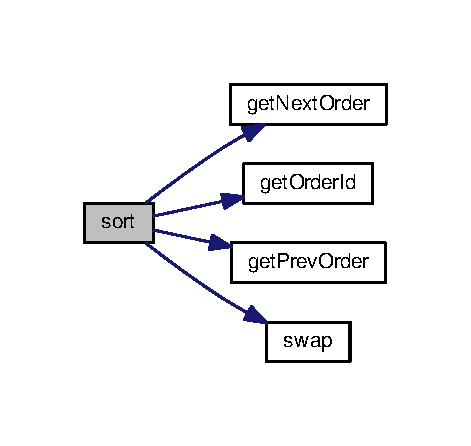
\includegraphics[width=226pt]{list_8c_a68123d7e3ab7016228af42c9ae480626_cgraph}
\end{center}
\end{figure}


\hypertarget{list_8c_a48838b111c5cba7f2503e6cb34992371}{\index{list.\-c@{list.\-c}!swap@{swap}}
\index{swap@{swap}!list.c@{list.\-c}}
\subsubsection[{swap}]{\setlength{\rightskip}{0pt plus 5cm}void swap (
\begin{DoxyParamCaption}
\item[{struct {\bf onode} $\ast$$\ast$}]{head, }
\item[{struct {\bf onode} $\ast$}]{node1, }
\item[{struct {\bf onode} $\ast$}]{node2}
\end{DoxyParamCaption}
)}}\label{list_8c_a48838b111c5cba7f2503e6cb34992371}


References onode\-::data.



Referenced by sort().



\subsection{Variable Documentation}
\hypertarget{list_8c_a71867e609034d4dbd6d0ad8d84540e59}{\index{list.\-c@{list.\-c}!g@{g}}
\index{g@{g}!list.c@{list.\-c}}
\subsubsection[{g}]{\setlength{\rightskip}{0pt plus 5cm}int g =0}}\label{list_8c_a71867e609034d4dbd6d0ad8d84540e59}


Referenced by new\-Node().


\hypertarget{list_8h}{\section{list/list.h File Reference}
\label{list_8h}\index{list/list.\-h@{list/list.\-h}}
}
This graph shows which files directly or indirectly include this file\-:\nopagebreak
\begin{figure}[H]
\begin{center}
\leavevmode
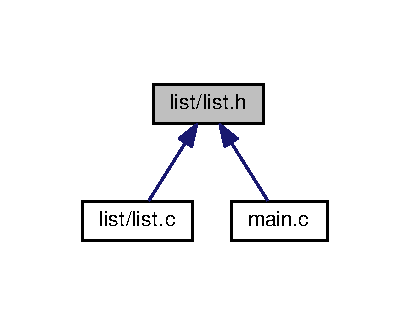
\includegraphics[width=197pt]{list_8h__dep__incl}
\end{center}
\end{figure}
\subsection*{Data Structures}
\begin{DoxyCompactItemize}
\item 
struct \hyperlink{structorder}{order}
\item 
struct \hyperlink{structonode}{onode}
\end{DoxyCompactItemize}
\subsection*{Functions}
\begin{DoxyCompactItemize}
\item 
struct \hyperlink{structonode}{onode} $\ast$ \hyperlink{list_8h_ace16262cb905d559225fe768d32d574b}{new\-Node} (struct \hyperlink{structorder}{order} $\ast$data)
\begin{DoxyCompactList}\small\item\em Returns a new linked list node filled in with the given order, The function allocates a new order and copy the values stored in data then allocate a linked list node. \end{DoxyCompactList}\item 
struct \hyperlink{structonode}{onode} $\ast$ \hyperlink{list_8h_ad0b81dec75f1c7bfca0ec9a6f9ae2f30}{new\-Node\-By\-Ref} (struct \hyperlink{structorder}{order} $\ast$data)
\begin{DoxyCompactList}\small\item\em Returns a new linked list node filled in with the given order, The function allocates a new order and copy the values stored in data then allocate a linked list node. \end{DoxyCompactList}\item 
void \hyperlink{list_8h_ab20a8a7735339bdced34d2d97304b583}{push\-Node} (struct \hyperlink{structonode}{onode} $\ast$$\ast$head, struct \hyperlink{structonode}{onode} $\ast$node)
\begin{DoxyCompactList}\small\item\em In a linked list with $\ast$head as the head pointer, adds the given node to the front of the list. \end{DoxyCompactList}\item 
struct \hyperlink{structonode}{onode} $\ast$ \hyperlink{list_8h_afd94ea6b6cb1035da16a95976a484ec8}{get\-Order\-Node} (struct \hyperlink{structonode}{onode} $\ast$head, int id)
\begin{DoxyCompactList}\small\item\em In a linked list with $\ast$head as the head pointer, returns the onode with the given order id. \end{DoxyCompactList}\item 
void \hyperlink{list_8h_aac2759a1682242fc31ec173316a40647}{insert\-Node} (struct \hyperlink{structonode}{onode} $\ast$$\ast$head, struct \hyperlink{structonode}{onode} $\ast$prev\-Node, struct \hyperlink{structonode}{onode} $\ast$inserting\-Node)
\begin{DoxyCompactList}\small\item\em Insert the given node after the prev\-Node. \end{DoxyCompactList}\item 
void \hyperlink{list_8h_a57726dc16efcab2ebe228494fce04bf0}{evict\-Node} (struct \hyperlink{structonode}{onode} $\ast$$\ast$head, struct \hyperlink{structonode}{onode} $\ast$node)
\begin{DoxyCompactList}\small\item\em Internally removes the specified node from the list, and updates the linked list. \end{DoxyCompactList}\item 
void \hyperlink{list_8h_a59bce7be7525819723563c7a5d83065f}{delete\-Node} (struct \hyperlink{structonode}{onode} $\ast$$\ast$head, struct \hyperlink{structonode}{onode} $\ast$node)
\begin{DoxyCompactList}\small\item\em Removes the specified node from the list, and frees all memory the node is using. \end{DoxyCompactList}\item 
void \hyperlink{list_8h_a440d2fb8a7f4399ae63fadcd19e67353}{delete\-Node\-Only} (struct \hyperlink{structonode}{onode} $\ast$$\ast$head, struct \hyperlink{structonode}{onode} $\ast$node)
\begin{DoxyCompactList}\small\item\em Removes the specified node from the list, and does N\-O\-T free memory the node is using. \end{DoxyCompactList}\item 
void \hyperlink{list_8h_afd387a5ae038d1e69411b6e5dee52bfe}{delete\-List} (struct \hyperlink{structonode}{onode} $\ast$$\ast$head)
\begin{DoxyCompactList}\small\item\em Deletes every node in the list with $\ast$head as the head pointer. \end{DoxyCompactList}\item 
void \hyperlink{list_8h_a1ca006182933095d94eb455540ff162d}{delete\-Just\-List} (struct \hyperlink{structonode}{onode} $\ast$$\ast$head)
\begin{DoxyCompactList}\small\item\em Deletes every node E\-X\-C\-E\-P\-T the head in the list with $\ast$head as the head pointer. \end{DoxyCompactList}\item 
void \hyperlink{list_8h_ac334adb29fda2c483930f77a871bc049}{print\-List} (struct \hyperlink{structonode}{onode} $\ast$node, void($\ast$print\-Item)(struct \hyperlink{structorder}{order} $\ast$, F\-I\-L\-E $\ast$), F\-I\-L\-E $\ast$out)
\end{DoxyCompactItemize}
\begin{Indent}{\bf group1 Content Management\-: Setters and Getters for linked\-List}\par
{\em Setters and Getters for linked\-List }\begin{DoxyCompactItemize}
\item 
struct \hyperlink{structonode}{onode} $\ast$ \hyperlink{list_8h_ace9faaeb801bbdf650d93f4a8b075c4c}{get\-Next\-Order} (struct \hyperlink{structonode}{onode} $\ast$order\-\_\-node)
\begin{DoxyCompactList}\small\item\em Simply returns the next node in the list, or N\-U\-L\-L if there are no further nodes. \end{DoxyCompactList}\item 
struct \hyperlink{structonode}{onode} $\ast$ \hyperlink{list_8h_a9960b22010f913d546f29222e8fe71c1}{get\-Prev\-Order} (struct \hyperlink{structonode}{onode} $\ast$order\-\_\-node)
\item 
struct \hyperlink{structorder}{order} $\ast$ \hyperlink{list_8h_a926f037e453969ff428e61cf5d0300ac}{get\-Order\-Data} (struct \hyperlink{structonode}{onode} $\ast$order\-\_\-node)
\end{DoxyCompactItemize}
\end{Indent}
\begin{Indent}{\bf group2 Content Management\-: Setters and Getters for order data}\par
{\em Setters and Getters for linked\-List }\begin{DoxyCompactItemize}
\item 
int \hyperlink{list_8h_a2eecdd9441c2808156e2823cf2647acf}{get\-Order\-Id} (struct \hyperlink{structorder}{order} $\ast$order\-Data)
\item 
char \hyperlink{list_8h_a73e537f55ebe8a58816876e8c62c0613}{get\-Order\-Startstop} (struct \hyperlink{structorder}{order} $\ast$order\-Data, char bank\-Num)
\item 
int \hyperlink{list_8h_a2300cf7be3777ca0d27069a65378d41d}{get\-Order\-Note} (struct \hyperlink{structorder}{order} $\ast$order\-Data, char bank\-Num)
\item 
void \hyperlink{list_8h_aa1c09c554716a9c9267e6bdea34f4040}{set\-Order\-Id} (struct \hyperlink{structorder}{order} $\ast$order\-Data, int id)
\item 
void \hyperlink{list_8h_a2772e75f849e208065637fb8e40816f6}{set\-Order\-Startstop} (struct \hyperlink{structorder}{order} $\ast$order\-Data, char new\-Startstop, char bank\-Num)
\item 
void \hyperlink{list_8h_ac4be440700d9a5aba95aab1486c043d6}{set\-Order\-Note} (struct \hyperlink{structorder}{order} $\ast$order\-Data, char new\-Note, char bank\-Num)
\end{DoxyCompactItemize}
\end{Indent}
\begin{Indent}{\bf group3 Sorting functions}\par
\begin{DoxyCompactItemize}
\item 
void \hyperlink{list_8h_a2619995556f99e9827e5be178b5d6ebd}{swap} (struct \hyperlink{structonode}{onode} $\ast$$\ast$head, struct \hyperlink{structonode}{onode} $\ast$n1, struct \hyperlink{structonode}{onode} $\ast$n2)
\item 
void \hyperlink{list_8h_a68123d7e3ab7016228af42c9ae480626}{sort} (struct \hyperlink{structonode}{onode} $\ast$$\ast$head)
\begin{DoxyCompactList}\small\item\em Performes insertion sort on the list by comparing the Order\-I\-D. \end{DoxyCompactList}\end{DoxyCompactItemize}
\end{Indent}


\subsection{Function Documentation}
\hypertarget{list_8h_a1ca006182933095d94eb455540ff162d}{\index{list.\-h@{list.\-h}!delete\-Just\-List@{delete\-Just\-List}}
\index{delete\-Just\-List@{delete\-Just\-List}!list.h@{list.\-h}}
\subsubsection[{delete\-Just\-List}]{\setlength{\rightskip}{0pt plus 5cm}void delete\-Just\-List (
\begin{DoxyParamCaption}
\item[{struct {\bf onode} $\ast$$\ast$}]{head}
\end{DoxyParamCaption}
)}}\label{list_8h_a1ca006182933095d94eb455540ff162d}


Deletes every node E\-X\-C\-E\-P\-T the head in the list with $\ast$head as the head pointer. 

After calling this function, all memory used by the list should be freed, and $\ast$head should be N\-U\-L\-L. 

References onode\-::next.

\hypertarget{list_8h_afd387a5ae038d1e69411b6e5dee52bfe}{\index{list.\-h@{list.\-h}!delete\-List@{delete\-List}}
\index{delete\-List@{delete\-List}!list.h@{list.\-h}}
\subsubsection[{delete\-List}]{\setlength{\rightskip}{0pt plus 5cm}void delete\-List (
\begin{DoxyParamCaption}
\item[{struct {\bf onode} $\ast$$\ast$}]{head}
\end{DoxyParamCaption}
)}}\label{list_8h_afd387a5ae038d1e69411b6e5dee52bfe}


Deletes every node in the list with $\ast$head as the head pointer. 

After calling this function, all memory used by the list should be freed, and $\ast$head should be N\-U\-L\-L. 

References onode\-::data, and onode\-::next.

\hypertarget{list_8h_a59bce7be7525819723563c7a5d83065f}{\index{list.\-h@{list.\-h}!delete\-Node@{delete\-Node}}
\index{delete\-Node@{delete\-Node}!list.h@{list.\-h}}
\subsubsection[{delete\-Node}]{\setlength{\rightskip}{0pt plus 5cm}void delete\-Node (
\begin{DoxyParamCaption}
\item[{struct {\bf onode} $\ast$$\ast$}]{head, }
\item[{struct {\bf onode} $\ast$}]{node}
\end{DoxyParamCaption}
)}}\label{list_8h_a59bce7be7525819723563c7a5d83065f}


Removes the specified node from the list, and frees all memory the node is using. 

Remember if $\ast$head is the node being deleted, it must be updated. 

References onode\-::data, and delete\-Node\-Only().



Here is the call graph for this function\-:
\nopagebreak
\begin{figure}[H]
\begin{center}
\leavevmode
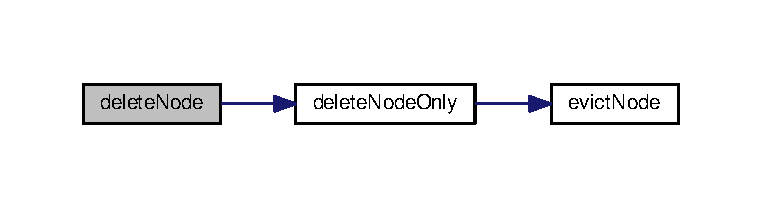
\includegraphics[width=350pt]{list_8h_a59bce7be7525819723563c7a5d83065f_cgraph}
\end{center}
\end{figure}


\hypertarget{list_8h_a440d2fb8a7f4399ae63fadcd19e67353}{\index{list.\-h@{list.\-h}!delete\-Node\-Only@{delete\-Node\-Only}}
\index{delete\-Node\-Only@{delete\-Node\-Only}!list.h@{list.\-h}}
\subsubsection[{delete\-Node\-Only}]{\setlength{\rightskip}{0pt plus 5cm}void delete\-Node\-Only (
\begin{DoxyParamCaption}
\item[{struct {\bf onode} $\ast$$\ast$}]{head, }
\item[{struct {\bf onode} $\ast$}]{node}
\end{DoxyParamCaption}
)}}\label{list_8h_a440d2fb8a7f4399ae63fadcd19e67353}


Removes the specified node from the list, and does N\-O\-T free memory the node is using. 

Remember if $\ast$head is the node being deleted, it must be updated. 

References evict\-Node().



Referenced by delete\-Node().



Here is the call graph for this function\-:
\nopagebreak
\begin{figure}[H]
\begin{center}
\leavevmode
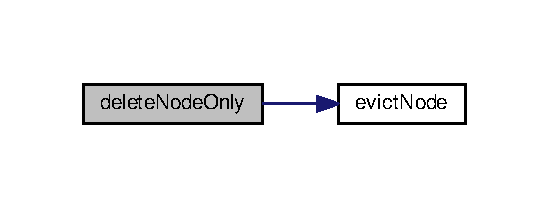
\includegraphics[width=264pt]{list_8h_a440d2fb8a7f4399ae63fadcd19e67353_cgraph}
\end{center}
\end{figure}


\hypertarget{list_8h_a57726dc16efcab2ebe228494fce04bf0}{\index{list.\-h@{list.\-h}!evict\-Node@{evict\-Node}}
\index{evict\-Node@{evict\-Node}!list.h@{list.\-h}}
\subsubsection[{evict\-Node}]{\setlength{\rightskip}{0pt plus 5cm}void evict\-Node (
\begin{DoxyParamCaption}
\item[{struct {\bf onode} $\ast$$\ast$}]{head, }
\item[{struct {\bf onode} $\ast$}]{node}
\end{DoxyParamCaption}
)}}\label{list_8h_a57726dc16efcab2ebe228494fce04bf0}


Internally removes the specified node from the list, and updates the linked list. 



References onode\-::next, and onode\-::prev.



Referenced by delete\-Node\-Only().

\hypertarget{list_8h_ace9faaeb801bbdf650d93f4a8b075c4c}{\index{list.\-h@{list.\-h}!get\-Next\-Order@{get\-Next\-Order}}
\index{get\-Next\-Order@{get\-Next\-Order}!list.h@{list.\-h}}
\subsubsection[{get\-Next\-Order}]{\setlength{\rightskip}{0pt plus 5cm}struct {\bf onode}$\ast$ get\-Next\-Order (
\begin{DoxyParamCaption}
\item[{struct {\bf onode} $\ast$}]{order\-\_\-node}
\end{DoxyParamCaption}
)}}\label{list_8h_ace9faaeb801bbdf650d93f4a8b075c4c}


Simply returns the next node in the list, or N\-U\-L\-L if there are no further nodes. 



References onode\-::next.



Referenced by sort().

\hypertarget{list_8h_a926f037e453969ff428e61cf5d0300ac}{\index{list.\-h@{list.\-h}!get\-Order\-Data@{get\-Order\-Data}}
\index{get\-Order\-Data@{get\-Order\-Data}!list.h@{list.\-h}}
\subsubsection[{get\-Order\-Data}]{\setlength{\rightskip}{0pt plus 5cm}struct {\bf order}$\ast$ get\-Order\-Data (
\begin{DoxyParamCaption}
\item[{struct {\bf onode} $\ast$}]{order\-\_\-node}
\end{DoxyParamCaption}
)}}\label{list_8h_a926f037e453969ff428e61cf5d0300ac}


References onode\-::data.

\hypertarget{list_8h_a2eecdd9441c2808156e2823cf2647acf}{\index{list.\-h@{list.\-h}!get\-Order\-Id@{get\-Order\-Id}}
\index{get\-Order\-Id@{get\-Order\-Id}!list.h@{list.\-h}}
\subsubsection[{get\-Order\-Id}]{\setlength{\rightskip}{0pt plus 5cm}int get\-Order\-Id (
\begin{DoxyParamCaption}
\item[{struct {\bf order} $\ast$}]{order\-Data}
\end{DoxyParamCaption}
)}}\label{list_8h_a2eecdd9441c2808156e2823cf2647acf}


References order\-::id.



Referenced by sort().

\hypertarget{list_8h_afd94ea6b6cb1035da16a95976a484ec8}{\index{list.\-h@{list.\-h}!get\-Order\-Node@{get\-Order\-Node}}
\index{get\-Order\-Node@{get\-Order\-Node}!list.h@{list.\-h}}
\subsubsection[{get\-Order\-Node}]{\setlength{\rightskip}{0pt plus 5cm}struct {\bf onode}$\ast$ get\-Order\-Node (
\begin{DoxyParamCaption}
\item[{struct {\bf onode} $\ast$}]{head, }
\item[{int}]{id}
\end{DoxyParamCaption}
)}}\label{list_8h_afd94ea6b6cb1035da16a95976a484ec8}


In a linked list with $\ast$head as the head pointer, returns the onode with the given order id. 

In a linked list with $\ast$head as the head pointer, returns the onode with the given order id.

If a node with the given word cannot be found, the function returns N\-U\-L\-L. 

References onode\-::data, order\-::id, and onode\-::next.

\hypertarget{list_8h_a2300cf7be3777ca0d27069a65378d41d}{\index{list.\-h@{list.\-h}!get\-Order\-Note@{get\-Order\-Note}}
\index{get\-Order\-Note@{get\-Order\-Note}!list.h@{list.\-h}}
\subsubsection[{get\-Order\-Note}]{\setlength{\rightskip}{0pt plus 5cm}int get\-Order\-Note (
\begin{DoxyParamCaption}
\item[{struct {\bf order} $\ast$}]{order\-Data, }
\item[{char}]{bank\-Num}
\end{DoxyParamCaption}
)}}\label{list_8h_a2300cf7be3777ca0d27069a65378d41d}


References order\-::bank1\-\_\-note, order\-::bank2\-\_\-note, and order\-::bank3\-\_\-note.

\hypertarget{list_8h_a73e537f55ebe8a58816876e8c62c0613}{\index{list.\-h@{list.\-h}!get\-Order\-Startstop@{get\-Order\-Startstop}}
\index{get\-Order\-Startstop@{get\-Order\-Startstop}!list.h@{list.\-h}}
\subsubsection[{get\-Order\-Startstop}]{\setlength{\rightskip}{0pt plus 5cm}char get\-Order\-Startstop (
\begin{DoxyParamCaption}
\item[{struct {\bf order} $\ast$}]{order\-Data, }
\item[{char}]{bank\-Num}
\end{DoxyParamCaption}
)}}\label{list_8h_a73e537f55ebe8a58816876e8c62c0613}


References order\-::bank1\-\_\-startstop, order\-::bank2\-\_\-startstop, and order\-::bank3\-\_\-startstop.

\hypertarget{list_8h_a9960b22010f913d546f29222e8fe71c1}{\index{list.\-h@{list.\-h}!get\-Prev\-Order@{get\-Prev\-Order}}
\index{get\-Prev\-Order@{get\-Prev\-Order}!list.h@{list.\-h}}
\subsubsection[{get\-Prev\-Order}]{\setlength{\rightskip}{0pt plus 5cm}struct {\bf onode}$\ast$ get\-Prev\-Order (
\begin{DoxyParamCaption}
\item[{struct {\bf onode} $\ast$}]{order\-\_\-node}
\end{DoxyParamCaption}
)}}\label{list_8h_a9960b22010f913d546f29222e8fe71c1}


References onode\-::prev.



Referenced by sort().

\hypertarget{list_8h_aac2759a1682242fc31ec173316a40647}{\index{list.\-h@{list.\-h}!insert\-Node@{insert\-Node}}
\index{insert\-Node@{insert\-Node}!list.h@{list.\-h}}
\subsubsection[{insert\-Node}]{\setlength{\rightskip}{0pt plus 5cm}void insert\-Node (
\begin{DoxyParamCaption}
\item[{struct {\bf onode} $\ast$$\ast$}]{head, }
\item[{struct {\bf onode} $\ast$}]{prev\-Node, }
\item[{struct {\bf onode} $\ast$}]{inserting\-Node}
\end{DoxyParamCaption}
)}}\label{list_8h_aac2759a1682242fc31ec173316a40647}


Insert the given node after the prev\-Node. 

If the prev\-Node is N\-U\-L\-L, then the given node is inserted at the head of the list. 

References onode\-::next, onode\-::prev, and push\-Node().



Here is the call graph for this function\-:
\nopagebreak
\begin{figure}[H]
\begin{center}
\leavevmode
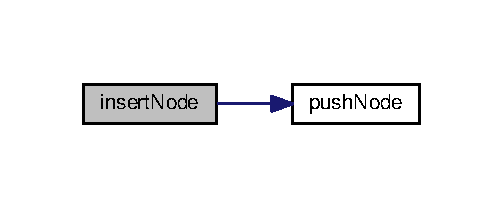
\includegraphics[width=242pt]{list_8h_aac2759a1682242fc31ec173316a40647_cgraph}
\end{center}
\end{figure}


\hypertarget{list_8h_ace16262cb905d559225fe768d32d574b}{\index{list.\-h@{list.\-h}!new\-Node@{new\-Node}}
\index{new\-Node@{new\-Node}!list.h@{list.\-h}}
\subsubsection[{new\-Node}]{\setlength{\rightskip}{0pt plus 5cm}struct {\bf onode}$\ast$ new\-Node (
\begin{DoxyParamCaption}
\item[{struct {\bf order} $\ast$}]{data}
\end{DoxyParamCaption}
)}}\label{list_8h_ace16262cb905d559225fe768d32d574b}


Returns a new linked list node filled in with the given order, The function allocates a new order and copy the values stored in data then allocate a linked list node. 

If you are implementing this function make sure that you duplicate, as the original data may be modified by the calling function.

Returns a new linked list node filled in with the given order, The function allocates a new order and copy the values stored in data then allocate a linked list node.

The order is copied into the node as a new instance. 

References order\-::bank1\-\_\-note, order\-::bank1\-\_\-startstop, order\-::bank2\-\_\-note, order\-::bank2\-\_\-startstop, order\-::bank3\-\_\-note, order\-::bank3\-\_\-startstop, g, and order\-::id.



Referenced by main().

\hypertarget{list_8h_ad0b81dec75f1c7bfca0ec9a6f9ae2f30}{\index{list.\-h@{list.\-h}!new\-Node\-By\-Ref@{new\-Node\-By\-Ref}}
\index{new\-Node\-By\-Ref@{new\-Node\-By\-Ref}!list.h@{list.\-h}}
\subsubsection[{new\-Node\-By\-Ref}]{\setlength{\rightskip}{0pt plus 5cm}struct {\bf onode}$\ast$ new\-Node\-By\-Ref (
\begin{DoxyParamCaption}
\item[{struct {\bf order} $\ast$}]{data}
\end{DoxyParamCaption}
)}}\label{list_8h_ad0b81dec75f1c7bfca0ec9a6f9ae2f30}


Returns a new linked list node filled in with the given order, The function allocates a new order and copy the values stored in data then allocate a linked list node. 

This function is different that new\-Node in that the new node is created by reference and not copied

Returns a new linked list node filled in with the given order, The function allocates a new order and copy the values stored in data then allocate a linked list node.

The order is inserted by reference. 

References onode\-::data.

\hypertarget{list_8h_ac334adb29fda2c483930f77a871bc049}{\index{list.\-h@{list.\-h}!print\-List@{print\-List}}
\index{print\-List@{print\-List}!list.h@{list.\-h}}
\subsubsection[{print\-List}]{\setlength{\rightskip}{0pt plus 5cm}void print\-List (
\begin{DoxyParamCaption}
\item[{struct {\bf onode} $\ast$}]{node, }
\item[{void($\ast$)(struct {\bf order} $\ast$, F\-I\-L\-E $\ast$)}]{print\-Item, }
\item[{F\-I\-L\-E $\ast$}]{out}
\end{DoxyParamCaption}
)}}\label{list_8h_ac334adb29fda2c483930f77a871bc049}


References onode\-::data, and onode\-::next.

\hypertarget{list_8h_ab20a8a7735339bdced34d2d97304b583}{\index{list.\-h@{list.\-h}!push\-Node@{push\-Node}}
\index{push\-Node@{push\-Node}!list.h@{list.\-h}}
\subsubsection[{push\-Node}]{\setlength{\rightskip}{0pt plus 5cm}void push\-Node (
\begin{DoxyParamCaption}
\item[{struct {\bf onode} $\ast$$\ast$}]{head, }
\item[{struct {\bf onode} $\ast$}]{node}
\end{DoxyParamCaption}
)}}\label{list_8h_ab20a8a7735339bdced34d2d97304b583}


In a linked list with $\ast$head as the head pointer, adds the given node to the front of the list. 



References onode\-::next, and onode\-::prev.



Referenced by insert\-Node(), and main().

\hypertarget{list_8h_aa1c09c554716a9c9267e6bdea34f4040}{\index{list.\-h@{list.\-h}!set\-Order\-Id@{set\-Order\-Id}}
\index{set\-Order\-Id@{set\-Order\-Id}!list.h@{list.\-h}}
\subsubsection[{set\-Order\-Id}]{\setlength{\rightskip}{0pt plus 5cm}void set\-Order\-Id (
\begin{DoxyParamCaption}
\item[{struct {\bf order} $\ast$}]{order\-Data, }
\item[{int}]{id}
\end{DoxyParamCaption}
)}}\label{list_8h_aa1c09c554716a9c9267e6bdea34f4040}


References order\-::id.

\hypertarget{list_8h_ac4be440700d9a5aba95aab1486c043d6}{\index{list.\-h@{list.\-h}!set\-Order\-Note@{set\-Order\-Note}}
\index{set\-Order\-Note@{set\-Order\-Note}!list.h@{list.\-h}}
\subsubsection[{set\-Order\-Note}]{\setlength{\rightskip}{0pt plus 5cm}void set\-Order\-Note (
\begin{DoxyParamCaption}
\item[{struct {\bf order} $\ast$}]{order\-Data, }
\item[{char}]{new\-Note, }
\item[{char}]{bank\-Num}
\end{DoxyParamCaption}
)}}\label{list_8h_ac4be440700d9a5aba95aab1486c043d6}


References order\-::bank1\-\_\-note, order\-::bank2\-\_\-note, and order\-::bank3\-\_\-note.

\hypertarget{list_8h_a2772e75f849e208065637fb8e40816f6}{\index{list.\-h@{list.\-h}!set\-Order\-Startstop@{set\-Order\-Startstop}}
\index{set\-Order\-Startstop@{set\-Order\-Startstop}!list.h@{list.\-h}}
\subsubsection[{set\-Order\-Startstop}]{\setlength{\rightskip}{0pt plus 5cm}void set\-Order\-Startstop (
\begin{DoxyParamCaption}
\item[{struct {\bf order} $\ast$}]{order\-Data, }
\item[{char}]{new\-Startstop, }
\item[{char}]{bank\-Num}
\end{DoxyParamCaption}
)}}\label{list_8h_a2772e75f849e208065637fb8e40816f6}


References order\-::bank1\-\_\-startstop, order\-::bank2\-\_\-startstop, and order\-::bank3\-\_\-startstop.

\hypertarget{list_8h_a68123d7e3ab7016228af42c9ae480626}{\index{list.\-h@{list.\-h}!sort@{sort}}
\index{sort@{sort}!list.h@{list.\-h}}
\subsubsection[{sort}]{\setlength{\rightskip}{0pt plus 5cm}void sort (
\begin{DoxyParamCaption}
\item[{struct {\bf onode} $\ast$$\ast$}]{head}
\end{DoxyParamCaption}
)}}\label{list_8h_a68123d7e3ab7016228af42c9ae480626}


Performes insertion sort on the list by comparing the Order\-I\-D. 

Sorts from largest(head) to smallest. 

References onode\-::data, get\-Next\-Order(), get\-Order\-Id(), get\-Prev\-Order(), and swap().



Referenced by main().



Here is the call graph for this function\-:
\nopagebreak
\begin{figure}[H]
\begin{center}
\leavevmode
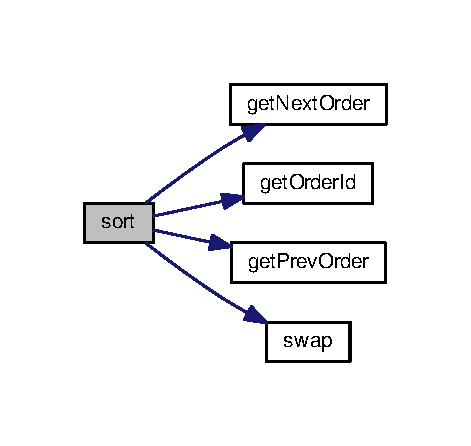
\includegraphics[width=226pt]{list_8h_a68123d7e3ab7016228af42c9ae480626_cgraph}
\end{center}
\end{figure}


\hypertarget{list_8h_a2619995556f99e9827e5be178b5d6ebd}{\index{list.\-h@{list.\-h}!swap@{swap}}
\index{swap@{swap}!list.h@{list.\-h}}
\subsubsection[{swap}]{\setlength{\rightskip}{0pt plus 5cm}void swap (
\begin{DoxyParamCaption}
\item[{struct {\bf onode} $\ast$$\ast$}]{head, }
\item[{struct {\bf onode} $\ast$}]{n1, }
\item[{struct {\bf onode} $\ast$}]{n2}
\end{DoxyParamCaption}
)}}\label{list_8h_a2619995556f99e9827e5be178b5d6ebd}


References onode\-::data.



Referenced by sort().


\hypertarget{main_8c}{\section{main.\-c File Reference}
\label{main_8c}\index{main.\-c@{main.\-c}}
}
{\ttfamily \#include \char`\"{}config.\-h\char`\"{}}\\*
{\ttfamily \#include $<$avr/io.\-h$>$}\\*
{\ttfamily \#include $<$avr/pgmspace.\-h$>$}\\*
{\ttfamily \#include $<$util/delay.\-h$>$}\\*
{\ttfamily \#include $<$stdio.\-h$>$}\\*
{\ttfamily \#include $<$string.\-h$>$}\\*
{\ttfamily \#include $<$stdlib.\-h$>$}\\*
{\ttfamily \#include \char`\"{}list/list.\-h\char`\"{}}\\*
{\ttfamily \#include \char`\"{}lcd8bit/lcd8bit.\-h\char`\"{}}\\*
{\ttfamily \#include \char`\"{}sd\-\_\-card/ff.\-h\char`\"{}}\\*
{\ttfamily \#include \char`\"{}sd\-\_\-card/integer.\-h\char`\"{}}\\*
{\ttfamily \#include \char`\"{}wavegen/wavegen.\-h\char`\"{}}\\*
{\ttfamily \#include \char`\"{}keyboard/keyboard.\-h\char`\"{}}\\*
Include dependency graph for main.\-c\-:\nopagebreak
\begin{figure}[H]
\begin{center}
\leavevmode
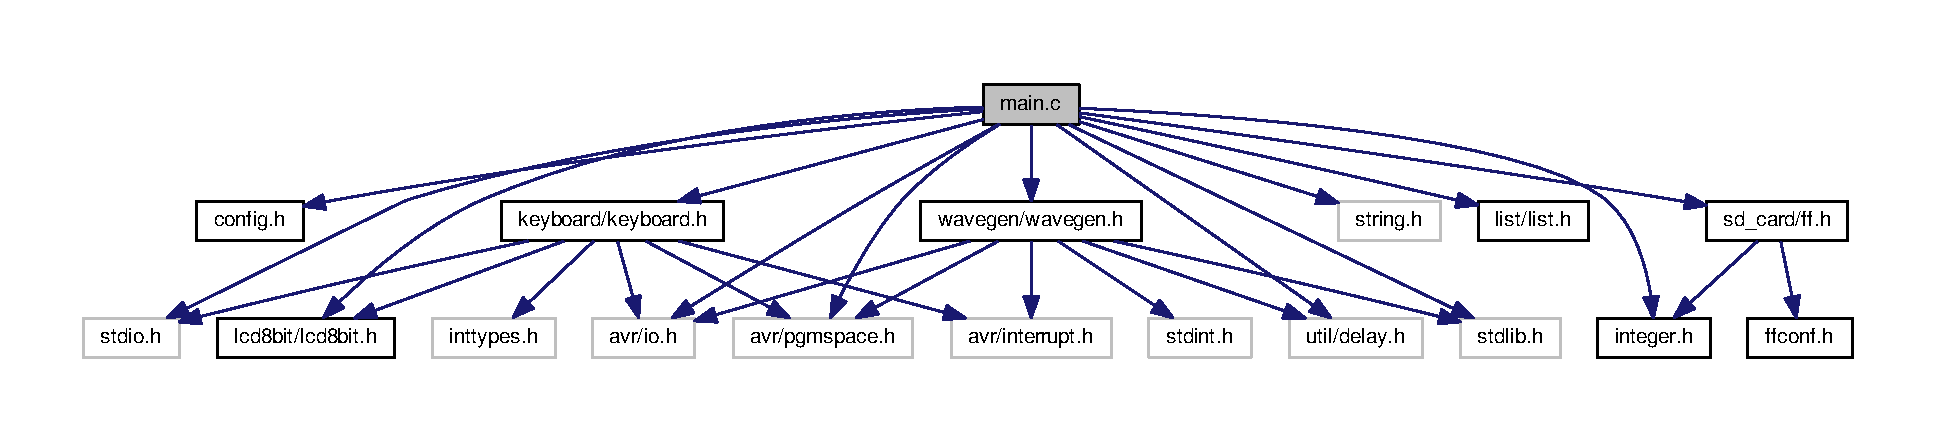
\includegraphics[width=350pt]{main_8c__incl}
\end{center}
\end{figure}
\subsection*{Functions}
\begin{DoxyCompactItemize}
\item 
\hyperlink{integer_8h_ad342ac907eb044443153a22f964bf0af}{D\-W\-O\-R\-D} \hyperlink{main_8c_af58b536abfd30f77213f4ecaf2ac52f5}{get\-\_\-fattime} (void)
\begin{DoxyCompactList}\small\item\em User Provided R\-T\-C Function called by Fat\-Fs module Used to provide a Timestamp for S\-D\-Card files and folders. \end{DoxyCompactList}\item 
void \hyperlink{main_8c_a3963feeee7b8bfeb3f34308a81c43663}{die} (char $\ast$message)
\begin{DoxyCompactList}\small\item\em Definations for wavegen library. \end{DoxyCompactList}\item 
int \hyperlink{main_8c_ae66f6b31b5ad750f1fe042a706a4e3d4}{main} ()
\end{DoxyCompactItemize}
\subsection*{Variables}
\begin{DoxyCompactItemize}
\item 
\hyperlink{structFATFS}{F\-A\-T\-F\-S} \hyperlink{main_8c_a8f47e042c2aca024c6534fdf5c3d9426}{Fat\-Fs}
\begin{DoxyCompactList}\small\item\em includes for linkedlist library \end{DoxyCompactList}\item 
\hyperlink{structFIL}{F\-I\-L} $\ast$ \hyperlink{main_8c_a8d839bbcaa5e21902d2481c87c4f359f}{fp}
\begin{DoxyCompactList}\small\item\em fpe object \end{DoxyCompactList}\end{DoxyCompactItemize}


\subsection{Function Documentation}
\hypertarget{main_8c_a3963feeee7b8bfeb3f34308a81c43663}{\index{main.\-c@{main.\-c}!die@{die}}
\index{die@{die}!main.c@{main.\-c}}
\subsubsection[{die}]{\setlength{\rightskip}{0pt plus 5cm}void die (
\begin{DoxyParamCaption}
\item[{char $\ast$}]{message}
\end{DoxyParamCaption}
)}}\label{main_8c_a3963feeee7b8bfeb3f34308a81c43663}


Definations for wavegen library. 

includes for P\-S/2 keyboard interface library End execution and display an error message on L\-C\-D 

References lcd\-\_\-clear\-\_\-and\-\_\-home(), lcd\-\_\-line\-\_\-one(), lcd\-\_\-line\-\_\-two(), and lcd\-\_\-write\-\_\-string\-\_\-0().



Referenced by main().



Here is the call graph for this function\-:
\nopagebreak
\begin{figure}[H]
\begin{center}
\leavevmode
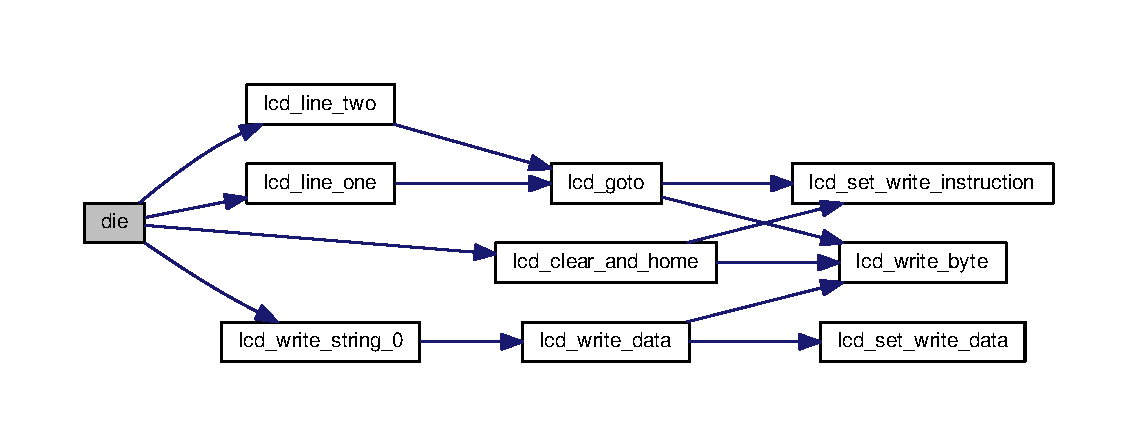
\includegraphics[width=350pt]{main_8c_a3963feeee7b8bfeb3f34308a81c43663_cgraph}
\end{center}
\end{figure}


\hypertarget{main_8c_af58b536abfd30f77213f4ecaf2ac52f5}{\index{main.\-c@{main.\-c}!get\-\_\-fattime@{get\-\_\-fattime}}
\index{get\-\_\-fattime@{get\-\_\-fattime}!main.c@{main.\-c}}
\subsubsection[{get\-\_\-fattime}]{\setlength{\rightskip}{0pt plus 5cm}{\bf D\-W\-O\-R\-D} get\-\_\-fattime (
\begin{DoxyParamCaption}
\item[{void}]{}
\end{DoxyParamCaption}
)}}\label{main_8c_af58b536abfd30f77213f4ecaf2ac52f5}


User Provided R\-T\-C Function called by Fat\-Fs module Used to provide a Timestamp for S\-D\-Card files and folders. 



Referenced by f\-\_\-open(), f\-\_\-setlabel(), and f\-\_\-sync().

\hypertarget{main_8c_ae66f6b31b5ad750f1fe042a706a4e3d4}{\index{main.\-c@{main.\-c}!main@{main}}
\index{main@{main}!main.c@{main.\-c}}
\subsubsection[{main}]{\setlength{\rightskip}{0pt plus 5cm}int main (
\begin{DoxyParamCaption}
{}
\end{DoxyParamCaption}
)}}\label{main_8c_ae66f6b31b5ad750f1fe042a706a4e3d4}


References order\-::bank1\-\_\-note, order\-::bank1\-\_\-startstop, order\-::bank2\-\_\-note, order\-::bank2\-\_\-startstop, order\-::bank3\-\_\-note, order\-::bank3\-\_\-startstop, char\-\_\-waiting, die(), f\-\_\-close(), f\-\_\-getlabel(), f\-\_\-mount(), f\-\_\-open(), f\-\_\-read(), f\-\_\-write(), F\-A\-\_\-\-C\-R\-E\-A\-T\-E\-\_\-\-A\-L\-W\-A\-Y\-S, F\-A\-\_\-\-R\-E\-A\-D, F\-A\-\_\-\-W\-R\-I\-T\-E, F\-R\-\_\-\-O\-K, order\-::id, keyboard\-\_\-init(), keyboard\-\_\-read\-\_\-char(), keyboard\-\_\-render\-\_\-scan\-\_\-code(), lcd\-\_\-clear\-\_\-and\-\_\-home(), lcd\-\_\-init(), lcd\-\_\-line\-\_\-one(), lcd\-\_\-line\-\_\-two(), lcd\-\_\-write\-\_\-string\-\_\-0(), new\-Node(), push\-Node(), release, sort(), wavegen\-\_\-clock\-\_\-init(), wavegen\-\_\-noise\-Wave(), wavegen\-\_\-pwm\-Init(), wavegen\-\_\-set\-Frequency(), wavegen\-\_\-set\-Frequency2(), wavegen\-\_\-set\-Sound(), and wavegen\-\_\-sine\-Wave().



Here is the call graph for this function\-:
\nopagebreak
\begin{figure}[H]
\begin{center}
\leavevmode
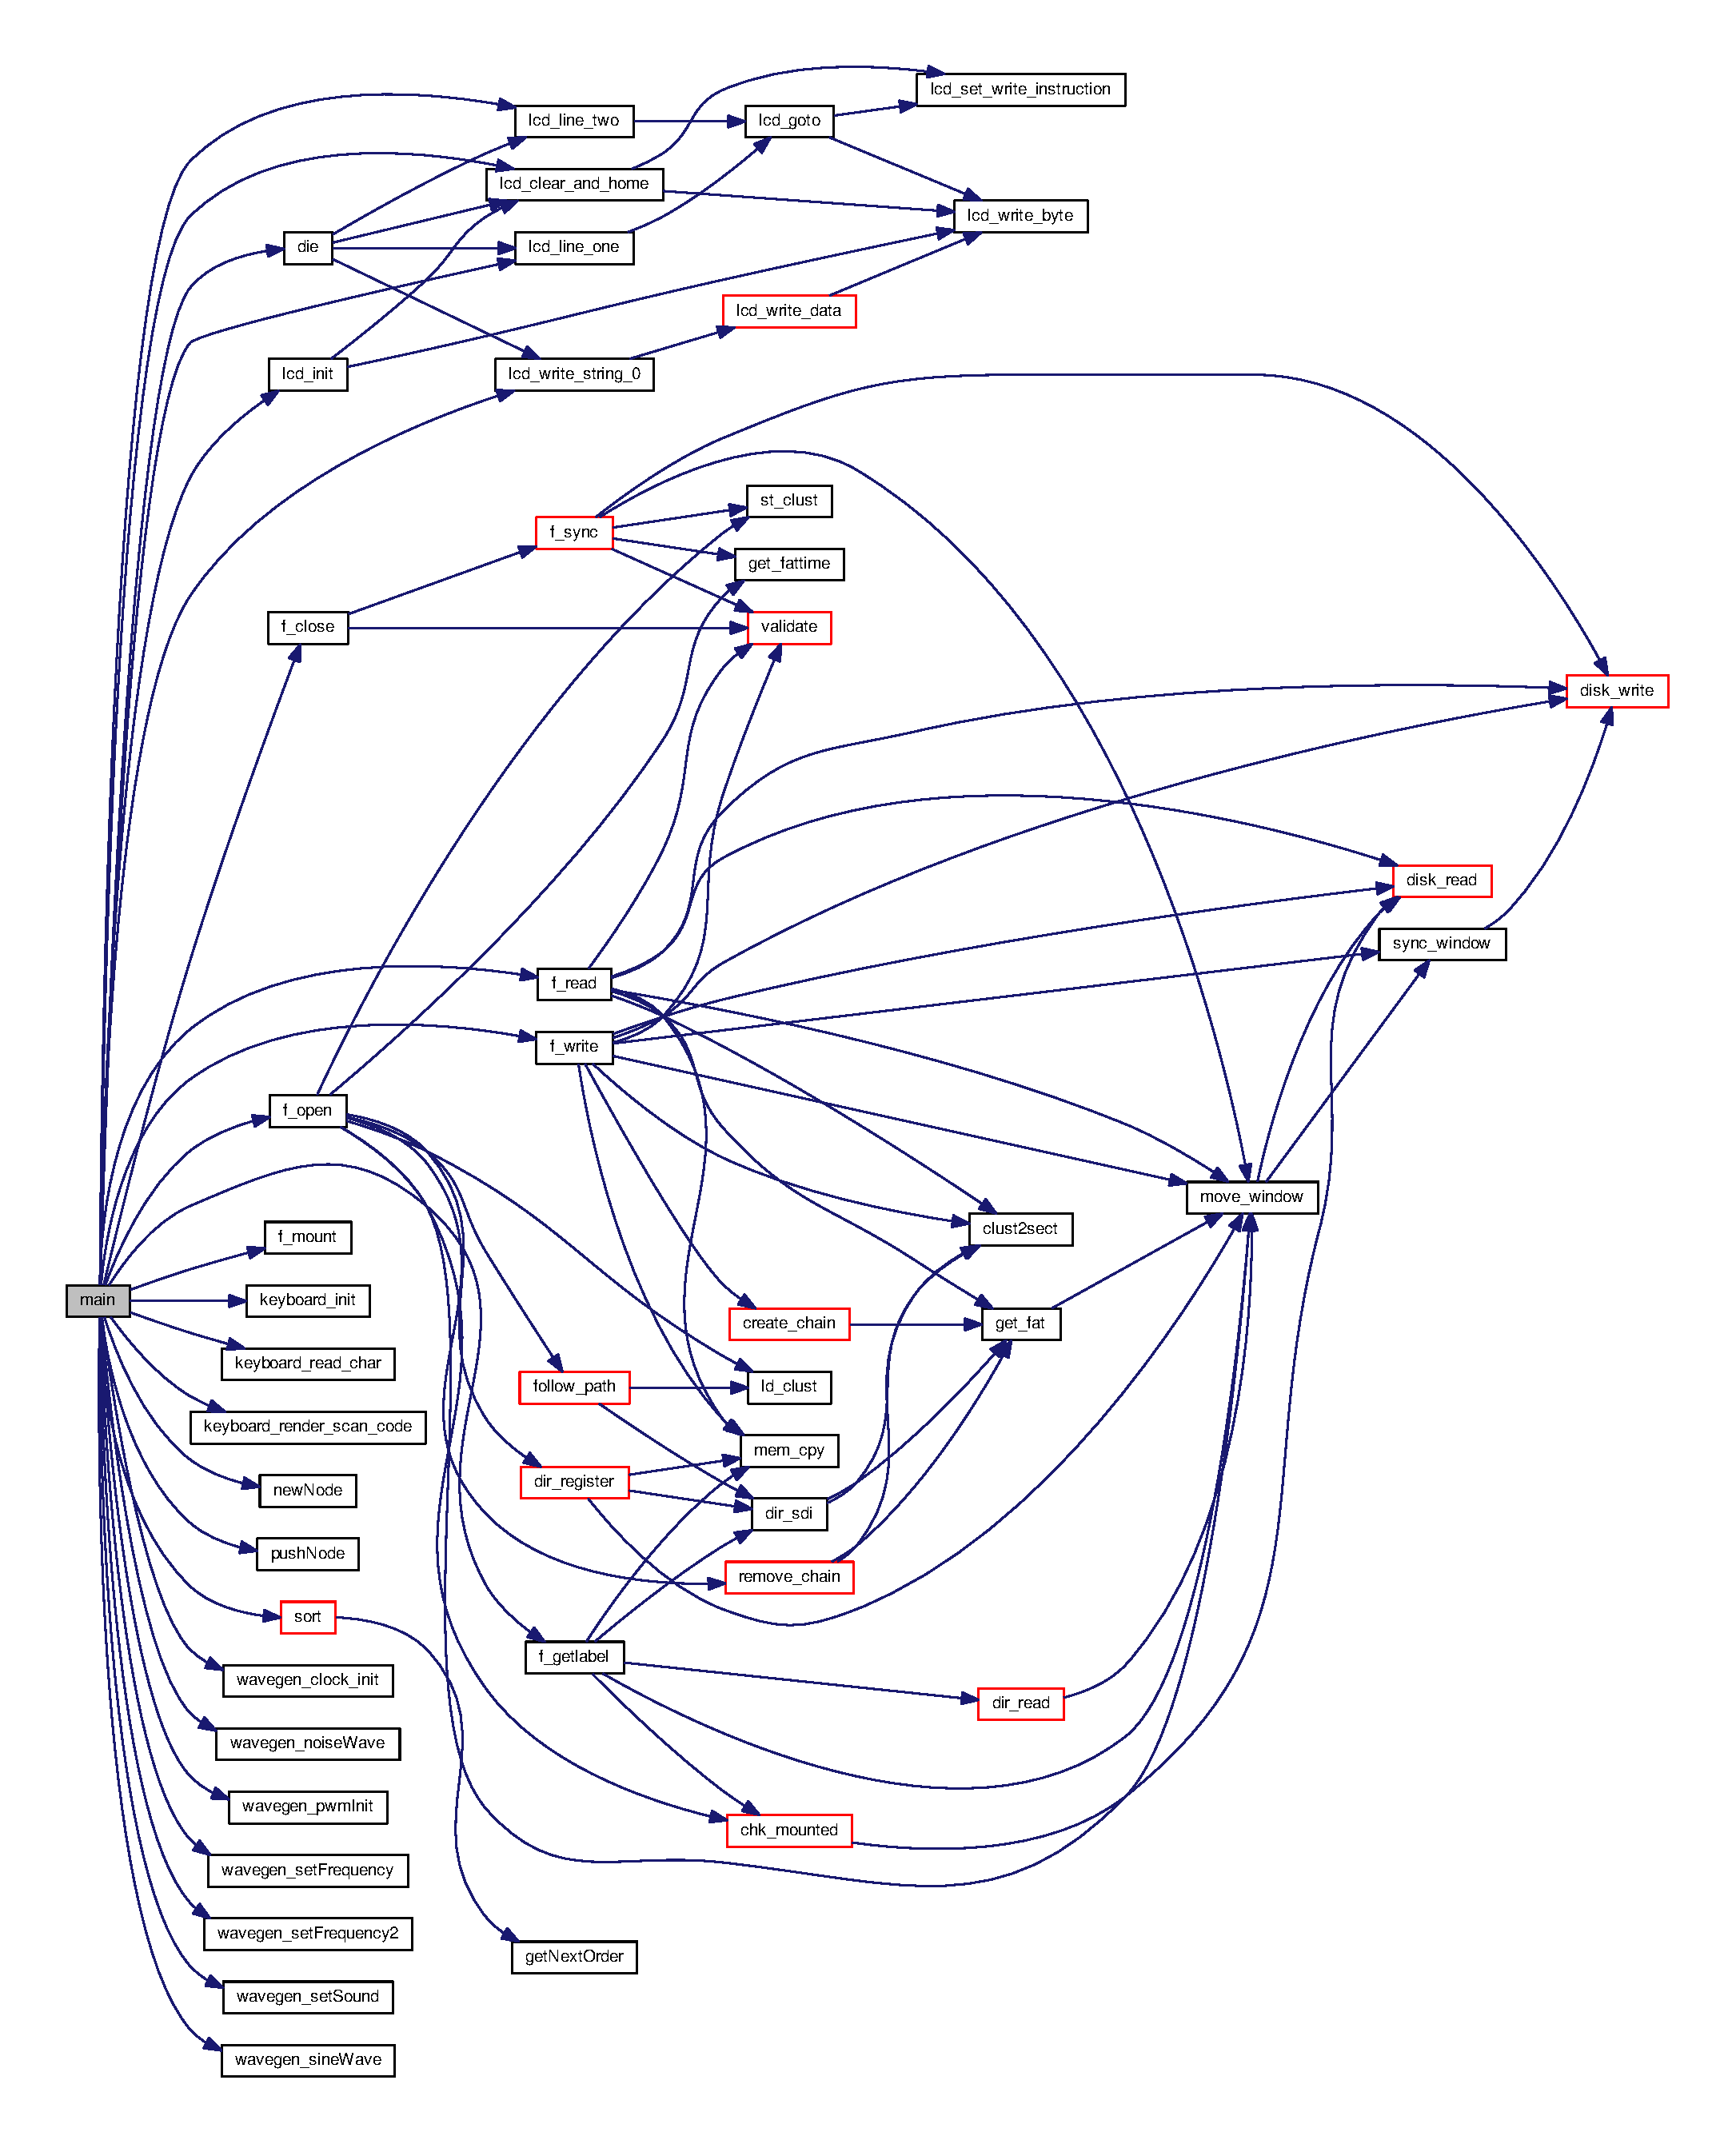
\includegraphics[width=350pt]{main_8c_ae66f6b31b5ad750f1fe042a706a4e3d4_cgraph}
\end{center}
\end{figure}




\subsection{Variable Documentation}
\hypertarget{main_8c_a8f47e042c2aca024c6534fdf5c3d9426}{\index{main.\-c@{main.\-c}!Fat\-Fs@{Fat\-Fs}}
\index{Fat\-Fs@{Fat\-Fs}!main.c@{main.\-c}}
\subsubsection[{Fat\-Fs}]{\setlength{\rightskip}{0pt plus 5cm}{\bf F\-A\-T\-F\-S} Fat\-Fs}}\label{main_8c_a8f47e042c2aca024c6534fdf5c3d9426}


includes for linkedlist library 

includes for lcd display library Definations for S\-D C\-A\-R\-D library\-Fat\-Fs work area \hypertarget{main_8c_a8d839bbcaa5e21902d2481c87c4f359f}{\index{main.\-c@{main.\-c}!fp@{fp}}
\index{fp@{fp}!main.c@{main.\-c}}
\subsubsection[{fp}]{\setlength{\rightskip}{0pt plus 5cm}{\bf F\-I\-L}$\ast$ fp}}\label{main_8c_a8d839bbcaa5e21902d2481c87c4f359f}


fpe object 


\hypertarget{Makefile}{\section{Makefile File Reference}
\label{Makefile}\index{Makefile@{Makefile}}
}
\subsection*{Variables}
\begin{DoxyCompactItemize}
\item 
\hyperlink{Makefile_a833b28f90e109607cd5d9e826474893a}{D\-E\-V\-I\-C\-E}
\item 
gc sections \hyperlink{Makefile_acbf05e6f0553ff348b66242ac5d80039}{Wl}
\end{DoxyCompactItemize}


\subsection{Variable Documentation}
\hypertarget{Makefile_a833b28f90e109607cd5d9e826474893a}{\index{Makefile@{Makefile}!D\-E\-V\-I\-C\-E@{D\-E\-V\-I\-C\-E}}
\index{D\-E\-V\-I\-C\-E@{D\-E\-V\-I\-C\-E}!Makefile@{Makefile}}
\subsubsection[{D\-E\-V\-I\-C\-E}]{\setlength{\rightskip}{0pt plus 5cm}D\-E\-V\-I\-C\-E}}\label{Makefile_a833b28f90e109607cd5d9e826474893a}
{\bfseries Initial value\-:}
\begin{DoxyCode}
=atxmega256d3
AVRDUDE\_DEVICE=x256d3

PROG= -c avrispmkII -P usb

CFLAGS=-\hyperlink{list_8c_a71867e609034d4dbd6d0ad8d84540e59}{g} -Wall -mcall-prologues -mmcu=$(\hyperlink{Makefile_a833b28f90e109607cd5d9e826474893a}{DEVICE}) -Os -std=c99 -fno-strict-aliasing
CC=avr-gcc
OBJ2HEX=avr-objcopy
LDFLAGS=-\hyperlink{Makefile_acbf05e6f0553ff348b66242ac5d80039}{Wl}
\end{DoxyCode}
\hypertarget{Makefile_acbf05e6f0553ff348b66242ac5d80039}{\index{Makefile@{Makefile}!Wl@{Wl}}
\index{Wl@{Wl}!Makefile@{Makefile}}
\subsubsection[{Wl}]{\setlength{\rightskip}{0pt plus 5cm}gc sections Wl}}\label{Makefile_acbf05e6f0553ff348b66242ac5d80039}

\hypertarget{diskio_8h}{\section{sd\-\_\-card/diskio.h File Reference}
\label{diskio_8h}\index{sd\-\_\-card/diskio.\-h@{sd\-\_\-card/diskio.\-h}}
}
{\ttfamily \#include \char`\"{}integer.\-h\char`\"{}}\\*
Include dependency graph for diskio.\-h\-:\nopagebreak
\begin{figure}[H]
\begin{center}
\leavevmode
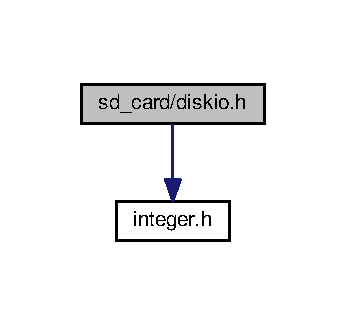
\includegraphics[width=166pt]{diskio_8h__incl}
\end{center}
\end{figure}
This graph shows which files directly or indirectly include this file\-:\nopagebreak
\begin{figure}[H]
\begin{center}
\leavevmode
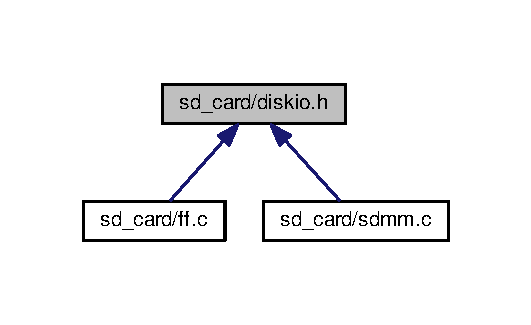
\includegraphics[width=255pt]{diskio_8h__dep__incl}
\end{center}
\end{figure}
\subsection*{Macros}
\begin{DoxyCompactItemize}
\item 
\#define \hyperlink{diskio_8h_abd6503c70d862b979a3f7080a59e9acd}{S\-T\-A\-\_\-\-N\-O\-I\-N\-I\-T}~0x01	/$\ast$ Drive not initialized $\ast$/
\item 
\#define \hyperlink{diskio_8h_aec625080763d6cf487e550a6c9a2dd19}{S\-T\-A\-\_\-\-N\-O\-D\-I\-S\-K}~0x02	/$\ast$ No medium in the drive $\ast$/
\item 
\#define \hyperlink{diskio_8h_a9ec6dc5f6620a33fabe388d3a111ca8c}{S\-T\-A\-\_\-\-P\-R\-O\-T\-E\-C\-T}~0x04	/$\ast$ Write protected $\ast$/
\item 
\#define \hyperlink{diskio_8h_a1b3c492f9aec325f0655941b75256f3c}{C\-T\-R\-L\-\_\-\-S\-Y\-N\-C}~0	/$\ast$ Flush disk cache (for write functions) $\ast$/
\item 
\#define \hyperlink{diskio_8h_a570216006f6a8fc4e1698b1bbb2d1dde}{G\-E\-T\-\_\-\-S\-E\-C\-T\-O\-R\-\_\-\-C\-O\-U\-N\-T}~1	/$\ast$ Get media size (for only \hyperlink{ff_8h_a7bead26ffb9a3b426bd42629ed6bf756}{f\-\_\-mkfs}()) $\ast$/
\item 
\#define \hyperlink{diskio_8h_aec3bb4dfe075d0ba2f3b07b300a95500}{G\-E\-T\-\_\-\-B\-L\-O\-C\-K\-\_\-\-S\-I\-Z\-E}~3	/$\ast$ Get erase block size (for only \hyperlink{ff_8h_a7bead26ffb9a3b426bd42629ed6bf756}{f\-\_\-mkfs}()) $\ast$/
\item 
\#define \hyperlink{diskio_8h_a3b1dc812217ea7ffa118b14a3c1ab151}{C\-T\-R\-L\-\_\-\-E\-R\-A\-S\-E\-\_\-\-S\-E\-C\-T\-O\-R}~4	/$\ast$ Force erased a block of sectors (for only \hyperlink{ffconf_8h_a0e697dc4206d98eac355ae878dcc286e}{\-\_\-\-U\-S\-E\-\_\-\-E\-R\-A\-S\-E}) $\ast$/
\item 
\#define \hyperlink{diskio_8h_a345531a07462afbd999f414708e3b65b}{C\-T\-R\-L\-\_\-\-P\-O\-W\-E\-R}~5	/$\ast$ Get/Set power status $\ast$/
\item 
\#define \hyperlink{diskio_8h_aba3a81a9a47c7d1bf3ac7749bc72dcfd}{M\-M\-C\-\_\-\-G\-E\-T\-\_\-\-T\-Y\-P\-E}~10	/$\ast$ Get card type $\ast$/
\item 
\#define \hyperlink{diskio_8h_ae3b858b81287929f7c7bea3b7aec3087}{M\-M\-C\-\_\-\-G\-E\-T\-\_\-\-C\-S\-D}~11	/$\ast$ Get C\-S\-D $\ast$/
\item 
\#define \hyperlink{diskio_8h_a17ad303dd18b19a4c90ab30a8a1c14c4}{M\-M\-C\-\_\-\-G\-E\-T\-\_\-\-C\-I\-D}~12	/$\ast$ Get C\-I\-D $\ast$/
\item 
\#define \hyperlink{diskio_8h_aff118ba6bd7a9fe7699cee049cff5d6c}{M\-M\-C\-\_\-\-G\-E\-T\-\_\-\-O\-C\-R}~13	/$\ast$ Get O\-C\-R $\ast$/
\item 
\#define \hyperlink{diskio_8h_a5cc43c8449b872e16ea5ab42592f793e}{M\-M\-C\-\_\-\-G\-E\-T\-\_\-\-S\-D\-S\-T\-A\-T}~14	/$\ast$ Get S\-D status $\ast$/
\item 
\#define \hyperlink{diskio_8h_a23f5fff3341e98825ea1f7367fd09f1a}{A\-T\-A\-\_\-\-G\-E\-T\-\_\-\-R\-E\-V}~20	/$\ast$ Get F/W revision $\ast$/
\item 
\#define \hyperlink{diskio_8h_a31f556ab98ab80c39058b38d9283865d}{A\-T\-A\-\_\-\-G\-E\-T\-\_\-\-M\-O\-D\-E\-L}~21	/$\ast$ Get model name $\ast$/
\item 
\#define \hyperlink{diskio_8h_a469c4f989757ee1ee404134fea3c74ba}{A\-T\-A\-\_\-\-G\-E\-T\-\_\-\-S\-N}~22	/$\ast$ Get serial number $\ast$/
\item 
\#define \hyperlink{diskio_8h_ac52ec66c278308382fdf7b2c57f0ad8c}{C\-T\-\_\-\-M\-M\-C}~0x01		/$\ast$ M\-M\-C ver 3 $\ast$/
\item 
\#define \hyperlink{diskio_8h_ad1c9fc863ec15d3320b3850dc571626e}{C\-T\-\_\-\-S\-D1}~0x02		/$\ast$ S\-D ver 1 $\ast$/
\item 
\#define \hyperlink{diskio_8h_a0db1b71113e73184a5ba511e7020a922}{C\-T\-\_\-\-S\-D2}~0x04		/$\ast$ S\-D ver 2 $\ast$/
\item 
\#define \hyperlink{diskio_8h_ae76d94ac83c68d1f025cb0bcad77fa5d}{C\-T\-\_\-\-S\-D\-C}~(\hyperlink{diskio_8h_ad1c9fc863ec15d3320b3850dc571626e}{C\-T\-\_\-\-S\-D1}$\vert$\hyperlink{diskio_8h_a0db1b71113e73184a5ba511e7020a922}{C\-T\-\_\-\-S\-D2})	/$\ast$ S\-D $\ast$/
\item 
\#define \hyperlink{diskio_8h_a7d48ce54c27f4f60666309e8627fab47}{C\-T\-\_\-\-B\-L\-O\-C\-K}~0x08		/$\ast$ Block addressing $\ast$/
\end{DoxyCompactItemize}
\subsection*{Typedefs}
\begin{DoxyCompactItemize}
\item 
typedef \hyperlink{integer_8h_a4ae1dab0fb4b072a66584546209e7d58}{B\-Y\-T\-E} \hyperlink{diskio_8h_adba6790898ce4029c20a34b898ce73c1}{D\-S\-T\-A\-T\-U\-S}
\end{DoxyCompactItemize}
\subsection*{Enumerations}
\begin{DoxyCompactItemize}
\item 
enum \hyperlink{diskio_8h_aacdfef1dad6565f65c26d12fe0ea4b2b}{D\-R\-E\-S\-U\-L\-T} \{ \\*
\hyperlink{diskio_8h_aacdfef1dad6565f65c26d12fe0ea4b2ba2ea4b6ef3fffc17dd1d38ab5c2837737}{R\-E\-S\-\_\-\-O\-K} = 0, 
\hyperlink{diskio_8h_aacdfef1dad6565f65c26d12fe0ea4b2ba78011f5557679ec178fb40bd21e89840}{R\-E\-S\-\_\-\-E\-R\-R\-O\-R}, 
\hyperlink{diskio_8h_aacdfef1dad6565f65c26d12fe0ea4b2ba442a6d4393dc404827067bc4e981b322}{R\-E\-S\-\_\-\-W\-R\-P\-R\-T}, 
\hyperlink{diskio_8h_aacdfef1dad6565f65c26d12fe0ea4b2baad64c27c69eb1ff39ae67c5f77bb2b1d}{R\-E\-S\-\_\-\-N\-O\-T\-R\-D\-Y}, 
\\*
\hyperlink{diskio_8h_aacdfef1dad6565f65c26d12fe0ea4b2baf4dcc07fd46310b5495fa8025c89a9f3}{R\-E\-S\-\_\-\-P\-A\-R\-E\-R\-R}
 \}
\end{DoxyCompactItemize}
\subsection*{Functions}
\begin{DoxyCompactItemize}
\item 
\hyperlink{diskio_8h_adba6790898ce4029c20a34b898ce73c1}{D\-S\-T\-A\-T\-U\-S} \hyperlink{diskio_8h_a09cdaa6f36fa409bdf002727bff98eb1}{disk\-\_\-initialize} (\hyperlink{integer_8h_a4ae1dab0fb4b072a66584546209e7d58}{B\-Y\-T\-E} pdrv)
\item 
\hyperlink{diskio_8h_adba6790898ce4029c20a34b898ce73c1}{D\-S\-T\-A\-T\-U\-S} \hyperlink{diskio_8h_a8348ac5ee6d709420c02e45c111f4793}{disk\-\_\-status} (\hyperlink{integer_8h_a4ae1dab0fb4b072a66584546209e7d58}{B\-Y\-T\-E} pdrv)
\item 
\hyperlink{diskio_8h_aacdfef1dad6565f65c26d12fe0ea4b2b}{D\-R\-E\-S\-U\-L\-T} \hyperlink{diskio_8h_ac0c802f8a12fa2047b4bec7109b9293f}{disk\-\_\-read} (\hyperlink{integer_8h_a4ae1dab0fb4b072a66584546209e7d58}{B\-Y\-T\-E} pdrv, \hyperlink{integer_8h_a4ae1dab0fb4b072a66584546209e7d58}{B\-Y\-T\-E} $\ast$buff, \hyperlink{integer_8h_ad342ac907eb044443153a22f964bf0af}{D\-W\-O\-R\-D} sector, \hyperlink{integer_8h_a4ae1dab0fb4b072a66584546209e7d58}{B\-Y\-T\-E} count)
\item 
\hyperlink{diskio_8h_aacdfef1dad6565f65c26d12fe0ea4b2b}{D\-R\-E\-S\-U\-L\-T} \hyperlink{diskio_8h_ac4785625f4bb82e33562079813659880}{disk\-\_\-write} (\hyperlink{integer_8h_a4ae1dab0fb4b072a66584546209e7d58}{B\-Y\-T\-E} pdrv, const \hyperlink{integer_8h_a4ae1dab0fb4b072a66584546209e7d58}{B\-Y\-T\-E} $\ast$buff, \hyperlink{integer_8h_ad342ac907eb044443153a22f964bf0af}{D\-W\-O\-R\-D} sector, \hyperlink{integer_8h_a4ae1dab0fb4b072a66584546209e7d58}{B\-Y\-T\-E} count)
\item 
\hyperlink{diskio_8h_aacdfef1dad6565f65c26d12fe0ea4b2b}{D\-R\-E\-S\-U\-L\-T} \hyperlink{diskio_8h_ab00fa450a811dbdabe3c655c1a36fab4}{disk\-\_\-ioctl} (\hyperlink{integer_8h_a4ae1dab0fb4b072a66584546209e7d58}{B\-Y\-T\-E} pdrv, \hyperlink{integer_8h_a4ae1dab0fb4b072a66584546209e7d58}{B\-Y\-T\-E} cmd, void $\ast$buff)
\end{DoxyCompactItemize}


\subsection{Macro Definition Documentation}
\hypertarget{diskio_8h_a31f556ab98ab80c39058b38d9283865d}{\index{diskio.\-h@{diskio.\-h}!A\-T\-A\-\_\-\-G\-E\-T\-\_\-\-M\-O\-D\-E\-L@{A\-T\-A\-\_\-\-G\-E\-T\-\_\-\-M\-O\-D\-E\-L}}
\index{A\-T\-A\-\_\-\-G\-E\-T\-\_\-\-M\-O\-D\-E\-L@{A\-T\-A\-\_\-\-G\-E\-T\-\_\-\-M\-O\-D\-E\-L}!diskio.h@{diskio.\-h}}
\subsubsection[{A\-T\-A\-\_\-\-G\-E\-T\-\_\-\-M\-O\-D\-E\-L}]{\setlength{\rightskip}{0pt plus 5cm}\#define A\-T\-A\-\_\-\-G\-E\-T\-\_\-\-M\-O\-D\-E\-L~21	/$\ast$ Get model name $\ast$/}}\label{diskio_8h_a31f556ab98ab80c39058b38d9283865d}
\hypertarget{diskio_8h_a23f5fff3341e98825ea1f7367fd09f1a}{\index{diskio.\-h@{diskio.\-h}!A\-T\-A\-\_\-\-G\-E\-T\-\_\-\-R\-E\-V@{A\-T\-A\-\_\-\-G\-E\-T\-\_\-\-R\-E\-V}}
\index{A\-T\-A\-\_\-\-G\-E\-T\-\_\-\-R\-E\-V@{A\-T\-A\-\_\-\-G\-E\-T\-\_\-\-R\-E\-V}!diskio.h@{diskio.\-h}}
\subsubsection[{A\-T\-A\-\_\-\-G\-E\-T\-\_\-\-R\-E\-V}]{\setlength{\rightskip}{0pt plus 5cm}\#define A\-T\-A\-\_\-\-G\-E\-T\-\_\-\-R\-E\-V~20	/$\ast$ Get F/W revision $\ast$/}}\label{diskio_8h_a23f5fff3341e98825ea1f7367fd09f1a}
\hypertarget{diskio_8h_a469c4f989757ee1ee404134fea3c74ba}{\index{diskio.\-h@{diskio.\-h}!A\-T\-A\-\_\-\-G\-E\-T\-\_\-\-S\-N@{A\-T\-A\-\_\-\-G\-E\-T\-\_\-\-S\-N}}
\index{A\-T\-A\-\_\-\-G\-E\-T\-\_\-\-S\-N@{A\-T\-A\-\_\-\-G\-E\-T\-\_\-\-S\-N}!diskio.h@{diskio.\-h}}
\subsubsection[{A\-T\-A\-\_\-\-G\-E\-T\-\_\-\-S\-N}]{\setlength{\rightskip}{0pt plus 5cm}\#define A\-T\-A\-\_\-\-G\-E\-T\-\_\-\-S\-N~22	/$\ast$ Get serial number $\ast$/}}\label{diskio_8h_a469c4f989757ee1ee404134fea3c74ba}
\hypertarget{diskio_8h_a7d48ce54c27f4f60666309e8627fab47}{\index{diskio.\-h@{diskio.\-h}!C\-T\-\_\-\-B\-L\-O\-C\-K@{C\-T\-\_\-\-B\-L\-O\-C\-K}}
\index{C\-T\-\_\-\-B\-L\-O\-C\-K@{C\-T\-\_\-\-B\-L\-O\-C\-K}!diskio.h@{diskio.\-h}}
\subsubsection[{C\-T\-\_\-\-B\-L\-O\-C\-K}]{\setlength{\rightskip}{0pt plus 5cm}\#define C\-T\-\_\-\-B\-L\-O\-C\-K~0x08		/$\ast$ Block addressing $\ast$/}}\label{diskio_8h_a7d48ce54c27f4f60666309e8627fab47}


Referenced by disk\-\_\-initialize(), disk\-\_\-read(), and disk\-\_\-write().

\hypertarget{diskio_8h_ac52ec66c278308382fdf7b2c57f0ad8c}{\index{diskio.\-h@{diskio.\-h}!C\-T\-\_\-\-M\-M\-C@{C\-T\-\_\-\-M\-M\-C}}
\index{C\-T\-\_\-\-M\-M\-C@{C\-T\-\_\-\-M\-M\-C}!diskio.h@{diskio.\-h}}
\subsubsection[{C\-T\-\_\-\-M\-M\-C}]{\setlength{\rightskip}{0pt plus 5cm}\#define C\-T\-\_\-\-M\-M\-C~0x01		/$\ast$ M\-M\-C ver 3 $\ast$/}}\label{diskio_8h_ac52ec66c278308382fdf7b2c57f0ad8c}


Referenced by disk\-\_\-initialize().

\hypertarget{diskio_8h_ad1c9fc863ec15d3320b3850dc571626e}{\index{diskio.\-h@{diskio.\-h}!C\-T\-\_\-\-S\-D1@{C\-T\-\_\-\-S\-D1}}
\index{C\-T\-\_\-\-S\-D1@{C\-T\-\_\-\-S\-D1}!diskio.h@{diskio.\-h}}
\subsubsection[{C\-T\-\_\-\-S\-D1}]{\setlength{\rightskip}{0pt plus 5cm}\#define C\-T\-\_\-\-S\-D1~0x02		/$\ast$ S\-D ver 1 $\ast$/}}\label{diskio_8h_ad1c9fc863ec15d3320b3850dc571626e}


Referenced by disk\-\_\-initialize().

\hypertarget{diskio_8h_a0db1b71113e73184a5ba511e7020a922}{\index{diskio.\-h@{diskio.\-h}!C\-T\-\_\-\-S\-D2@{C\-T\-\_\-\-S\-D2}}
\index{C\-T\-\_\-\-S\-D2@{C\-T\-\_\-\-S\-D2}!diskio.h@{diskio.\-h}}
\subsubsection[{C\-T\-\_\-\-S\-D2}]{\setlength{\rightskip}{0pt plus 5cm}\#define C\-T\-\_\-\-S\-D2~0x04		/$\ast$ S\-D ver 2 $\ast$/}}\label{diskio_8h_a0db1b71113e73184a5ba511e7020a922}


Referenced by disk\-\_\-initialize().

\hypertarget{diskio_8h_ae76d94ac83c68d1f025cb0bcad77fa5d}{\index{diskio.\-h@{diskio.\-h}!C\-T\-\_\-\-S\-D\-C@{C\-T\-\_\-\-S\-D\-C}}
\index{C\-T\-\_\-\-S\-D\-C@{C\-T\-\_\-\-S\-D\-C}!diskio.h@{diskio.\-h}}
\subsubsection[{C\-T\-\_\-\-S\-D\-C}]{\setlength{\rightskip}{0pt plus 5cm}\#define C\-T\-\_\-\-S\-D\-C~({\bf C\-T\-\_\-\-S\-D1}$\vert${\bf C\-T\-\_\-\-S\-D2})	/$\ast$ S\-D $\ast$/}}\label{diskio_8h_ae76d94ac83c68d1f025cb0bcad77fa5d}


Referenced by disk\-\_\-write().

\hypertarget{diskio_8h_a3b1dc812217ea7ffa118b14a3c1ab151}{\index{diskio.\-h@{diskio.\-h}!C\-T\-R\-L\-\_\-\-E\-R\-A\-S\-E\-\_\-\-S\-E\-C\-T\-O\-R@{C\-T\-R\-L\-\_\-\-E\-R\-A\-S\-E\-\_\-\-S\-E\-C\-T\-O\-R}}
\index{C\-T\-R\-L\-\_\-\-E\-R\-A\-S\-E\-\_\-\-S\-E\-C\-T\-O\-R@{C\-T\-R\-L\-\_\-\-E\-R\-A\-S\-E\-\_\-\-S\-E\-C\-T\-O\-R}!diskio.h@{diskio.\-h}}
\subsubsection[{C\-T\-R\-L\-\_\-\-E\-R\-A\-S\-E\-\_\-\-S\-E\-C\-T\-O\-R}]{\setlength{\rightskip}{0pt plus 5cm}\#define C\-T\-R\-L\-\_\-\-E\-R\-A\-S\-E\-\_\-\-S\-E\-C\-T\-O\-R~4	/$\ast$ Force erased a block of sectors (for only {\bf \-\_\-\-U\-S\-E\-\_\-\-E\-R\-A\-S\-E}) $\ast$/}}\label{diskio_8h_a3b1dc812217ea7ffa118b14a3c1ab151}


Referenced by remove\-\_\-chain().

\hypertarget{diskio_8h_a345531a07462afbd999f414708e3b65b}{\index{diskio.\-h@{diskio.\-h}!C\-T\-R\-L\-\_\-\-P\-O\-W\-E\-R@{C\-T\-R\-L\-\_\-\-P\-O\-W\-E\-R}}
\index{C\-T\-R\-L\-\_\-\-P\-O\-W\-E\-R@{C\-T\-R\-L\-\_\-\-P\-O\-W\-E\-R}!diskio.h@{diskio.\-h}}
\subsubsection[{C\-T\-R\-L\-\_\-\-P\-O\-W\-E\-R}]{\setlength{\rightskip}{0pt plus 5cm}\#define C\-T\-R\-L\-\_\-\-P\-O\-W\-E\-R~5	/$\ast$ Get/Set power status $\ast$/}}\label{diskio_8h_a345531a07462afbd999f414708e3b65b}
\hypertarget{diskio_8h_a1b3c492f9aec325f0655941b75256f3c}{\index{diskio.\-h@{diskio.\-h}!C\-T\-R\-L\-\_\-\-S\-Y\-N\-C@{C\-T\-R\-L\-\_\-\-S\-Y\-N\-C}}
\index{C\-T\-R\-L\-\_\-\-S\-Y\-N\-C@{C\-T\-R\-L\-\_\-\-S\-Y\-N\-C}!diskio.h@{diskio.\-h}}
\subsubsection[{C\-T\-R\-L\-\_\-\-S\-Y\-N\-C}]{\setlength{\rightskip}{0pt plus 5cm}\#define C\-T\-R\-L\-\_\-\-S\-Y\-N\-C~0	/$\ast$ Flush disk cache (for write functions) $\ast$/}}\label{diskio_8h_a1b3c492f9aec325f0655941b75256f3c}


Referenced by disk\-\_\-ioctl(), and sync\-\_\-fs().

\hypertarget{diskio_8h_aec3bb4dfe075d0ba2f3b07b300a95500}{\index{diskio.\-h@{diskio.\-h}!G\-E\-T\-\_\-\-B\-L\-O\-C\-K\-\_\-\-S\-I\-Z\-E@{G\-E\-T\-\_\-\-B\-L\-O\-C\-K\-\_\-\-S\-I\-Z\-E}}
\index{G\-E\-T\-\_\-\-B\-L\-O\-C\-K\-\_\-\-S\-I\-Z\-E@{G\-E\-T\-\_\-\-B\-L\-O\-C\-K\-\_\-\-S\-I\-Z\-E}!diskio.h@{diskio.\-h}}
\subsubsection[{G\-E\-T\-\_\-\-B\-L\-O\-C\-K\-\_\-\-S\-I\-Z\-E}]{\setlength{\rightskip}{0pt plus 5cm}\#define G\-E\-T\-\_\-\-B\-L\-O\-C\-K\-\_\-\-S\-I\-Z\-E~3	/$\ast$ Get erase block size (for only {\bf f\-\_\-mkfs}()) $\ast$/}}\label{diskio_8h_aec3bb4dfe075d0ba2f3b07b300a95500}


Referenced by disk\-\_\-ioctl().

\hypertarget{diskio_8h_a570216006f6a8fc4e1698b1bbb2d1dde}{\index{diskio.\-h@{diskio.\-h}!G\-E\-T\-\_\-\-S\-E\-C\-T\-O\-R\-\_\-\-C\-O\-U\-N\-T@{G\-E\-T\-\_\-\-S\-E\-C\-T\-O\-R\-\_\-\-C\-O\-U\-N\-T}}
\index{G\-E\-T\-\_\-\-S\-E\-C\-T\-O\-R\-\_\-\-C\-O\-U\-N\-T@{G\-E\-T\-\_\-\-S\-E\-C\-T\-O\-R\-\_\-\-C\-O\-U\-N\-T}!diskio.h@{diskio.\-h}}
\subsubsection[{G\-E\-T\-\_\-\-S\-E\-C\-T\-O\-R\-\_\-\-C\-O\-U\-N\-T}]{\setlength{\rightskip}{0pt plus 5cm}\#define G\-E\-T\-\_\-\-S\-E\-C\-T\-O\-R\-\_\-\-C\-O\-U\-N\-T~1	/$\ast$ Get media size (for only {\bf f\-\_\-mkfs}()) $\ast$/}}\label{diskio_8h_a570216006f6a8fc4e1698b1bbb2d1dde}


Referenced by disk\-\_\-ioctl().

\hypertarget{diskio_8h_a17ad303dd18b19a4c90ab30a8a1c14c4}{\index{diskio.\-h@{diskio.\-h}!M\-M\-C\-\_\-\-G\-E\-T\-\_\-\-C\-I\-D@{M\-M\-C\-\_\-\-G\-E\-T\-\_\-\-C\-I\-D}}
\index{M\-M\-C\-\_\-\-G\-E\-T\-\_\-\-C\-I\-D@{M\-M\-C\-\_\-\-G\-E\-T\-\_\-\-C\-I\-D}!diskio.h@{diskio.\-h}}
\subsubsection[{M\-M\-C\-\_\-\-G\-E\-T\-\_\-\-C\-I\-D}]{\setlength{\rightskip}{0pt plus 5cm}\#define M\-M\-C\-\_\-\-G\-E\-T\-\_\-\-C\-I\-D~12	/$\ast$ Get C\-I\-D $\ast$/}}\label{diskio_8h_a17ad303dd18b19a4c90ab30a8a1c14c4}
\hypertarget{diskio_8h_ae3b858b81287929f7c7bea3b7aec3087}{\index{diskio.\-h@{diskio.\-h}!M\-M\-C\-\_\-\-G\-E\-T\-\_\-\-C\-S\-D@{M\-M\-C\-\_\-\-G\-E\-T\-\_\-\-C\-S\-D}}
\index{M\-M\-C\-\_\-\-G\-E\-T\-\_\-\-C\-S\-D@{M\-M\-C\-\_\-\-G\-E\-T\-\_\-\-C\-S\-D}!diskio.h@{diskio.\-h}}
\subsubsection[{M\-M\-C\-\_\-\-G\-E\-T\-\_\-\-C\-S\-D}]{\setlength{\rightskip}{0pt plus 5cm}\#define M\-M\-C\-\_\-\-G\-E\-T\-\_\-\-C\-S\-D~11	/$\ast$ Get C\-S\-D $\ast$/}}\label{diskio_8h_ae3b858b81287929f7c7bea3b7aec3087}
\hypertarget{diskio_8h_aff118ba6bd7a9fe7699cee049cff5d6c}{\index{diskio.\-h@{diskio.\-h}!M\-M\-C\-\_\-\-G\-E\-T\-\_\-\-O\-C\-R@{M\-M\-C\-\_\-\-G\-E\-T\-\_\-\-O\-C\-R}}
\index{M\-M\-C\-\_\-\-G\-E\-T\-\_\-\-O\-C\-R@{M\-M\-C\-\_\-\-G\-E\-T\-\_\-\-O\-C\-R}!diskio.h@{diskio.\-h}}
\subsubsection[{M\-M\-C\-\_\-\-G\-E\-T\-\_\-\-O\-C\-R}]{\setlength{\rightskip}{0pt plus 5cm}\#define M\-M\-C\-\_\-\-G\-E\-T\-\_\-\-O\-C\-R~13	/$\ast$ Get O\-C\-R $\ast$/}}\label{diskio_8h_aff118ba6bd7a9fe7699cee049cff5d6c}
\hypertarget{diskio_8h_a5cc43c8449b872e16ea5ab42592f793e}{\index{diskio.\-h@{diskio.\-h}!M\-M\-C\-\_\-\-G\-E\-T\-\_\-\-S\-D\-S\-T\-A\-T@{M\-M\-C\-\_\-\-G\-E\-T\-\_\-\-S\-D\-S\-T\-A\-T}}
\index{M\-M\-C\-\_\-\-G\-E\-T\-\_\-\-S\-D\-S\-T\-A\-T@{M\-M\-C\-\_\-\-G\-E\-T\-\_\-\-S\-D\-S\-T\-A\-T}!diskio.h@{diskio.\-h}}
\subsubsection[{M\-M\-C\-\_\-\-G\-E\-T\-\_\-\-S\-D\-S\-T\-A\-T}]{\setlength{\rightskip}{0pt plus 5cm}\#define M\-M\-C\-\_\-\-G\-E\-T\-\_\-\-S\-D\-S\-T\-A\-T~14	/$\ast$ Get S\-D status $\ast$/}}\label{diskio_8h_a5cc43c8449b872e16ea5ab42592f793e}
\hypertarget{diskio_8h_aba3a81a9a47c7d1bf3ac7749bc72dcfd}{\index{diskio.\-h@{diskio.\-h}!M\-M\-C\-\_\-\-G\-E\-T\-\_\-\-T\-Y\-P\-E@{M\-M\-C\-\_\-\-G\-E\-T\-\_\-\-T\-Y\-P\-E}}
\index{M\-M\-C\-\_\-\-G\-E\-T\-\_\-\-T\-Y\-P\-E@{M\-M\-C\-\_\-\-G\-E\-T\-\_\-\-T\-Y\-P\-E}!diskio.h@{diskio.\-h}}
\subsubsection[{M\-M\-C\-\_\-\-G\-E\-T\-\_\-\-T\-Y\-P\-E}]{\setlength{\rightskip}{0pt plus 5cm}\#define M\-M\-C\-\_\-\-G\-E\-T\-\_\-\-T\-Y\-P\-E~10	/$\ast$ Get card type $\ast$/}}\label{diskio_8h_aba3a81a9a47c7d1bf3ac7749bc72dcfd}
\hypertarget{diskio_8h_aec625080763d6cf487e550a6c9a2dd19}{\index{diskio.\-h@{diskio.\-h}!S\-T\-A\-\_\-\-N\-O\-D\-I\-S\-K@{S\-T\-A\-\_\-\-N\-O\-D\-I\-S\-K}}
\index{S\-T\-A\-\_\-\-N\-O\-D\-I\-S\-K@{S\-T\-A\-\_\-\-N\-O\-D\-I\-S\-K}!diskio.h@{diskio.\-h}}
\subsubsection[{S\-T\-A\-\_\-\-N\-O\-D\-I\-S\-K}]{\setlength{\rightskip}{0pt plus 5cm}\#define S\-T\-A\-\_\-\-N\-O\-D\-I\-S\-K~0x02	/$\ast$ No medium in the drive $\ast$/}}\label{diskio_8h_aec625080763d6cf487e550a6c9a2dd19}
\hypertarget{diskio_8h_abd6503c70d862b979a3f7080a59e9acd}{\index{diskio.\-h@{diskio.\-h}!S\-T\-A\-\_\-\-N\-O\-I\-N\-I\-T@{S\-T\-A\-\_\-\-N\-O\-I\-N\-I\-T}}
\index{S\-T\-A\-\_\-\-N\-O\-I\-N\-I\-T@{S\-T\-A\-\_\-\-N\-O\-I\-N\-I\-T}!diskio.h@{diskio.\-h}}
\subsubsection[{S\-T\-A\-\_\-\-N\-O\-I\-N\-I\-T}]{\setlength{\rightskip}{0pt plus 5cm}\#define S\-T\-A\-\_\-\-N\-O\-I\-N\-I\-T~0x01	/$\ast$ Drive not initialized $\ast$/}}\label{diskio_8h_abd6503c70d862b979a3f7080a59e9acd}


Referenced by chk\-\_\-mounted(), disk\-\_\-initialize(), disk\-\_\-ioctl(), disk\-\_\-read(), disk\-\_\-status(), disk\-\_\-write(), and validate().

\hypertarget{diskio_8h_a9ec6dc5f6620a33fabe388d3a111ca8c}{\index{diskio.\-h@{diskio.\-h}!S\-T\-A\-\_\-\-P\-R\-O\-T\-E\-C\-T@{S\-T\-A\-\_\-\-P\-R\-O\-T\-E\-C\-T}}
\index{S\-T\-A\-\_\-\-P\-R\-O\-T\-E\-C\-T@{S\-T\-A\-\_\-\-P\-R\-O\-T\-E\-C\-T}!diskio.h@{diskio.\-h}}
\subsubsection[{S\-T\-A\-\_\-\-P\-R\-O\-T\-E\-C\-T}]{\setlength{\rightskip}{0pt plus 5cm}\#define S\-T\-A\-\_\-\-P\-R\-O\-T\-E\-C\-T~0x04	/$\ast$ Write protected $\ast$/}}\label{diskio_8h_a9ec6dc5f6620a33fabe388d3a111ca8c}


Referenced by chk\-\_\-mounted().



\subsection{Typedef Documentation}
\hypertarget{diskio_8h_adba6790898ce4029c20a34b898ce73c1}{\index{diskio.\-h@{diskio.\-h}!D\-S\-T\-A\-T\-U\-S@{D\-S\-T\-A\-T\-U\-S}}
\index{D\-S\-T\-A\-T\-U\-S@{D\-S\-T\-A\-T\-U\-S}!diskio.h@{diskio.\-h}}
\subsubsection[{D\-S\-T\-A\-T\-U\-S}]{\setlength{\rightskip}{0pt plus 5cm}typedef {\bf B\-Y\-T\-E} {\bf D\-S\-T\-A\-T\-U\-S}}}\label{diskio_8h_adba6790898ce4029c20a34b898ce73c1}


\subsection{Enumeration Type Documentation}
\hypertarget{diskio_8h_aacdfef1dad6565f65c26d12fe0ea4b2b}{\index{diskio.\-h@{diskio.\-h}!D\-R\-E\-S\-U\-L\-T@{D\-R\-E\-S\-U\-L\-T}}
\index{D\-R\-E\-S\-U\-L\-T@{D\-R\-E\-S\-U\-L\-T}!diskio.h@{diskio.\-h}}
\subsubsection[{D\-R\-E\-S\-U\-L\-T}]{\setlength{\rightskip}{0pt plus 5cm}enum {\bf D\-R\-E\-S\-U\-L\-T}}}\label{diskio_8h_aacdfef1dad6565f65c26d12fe0ea4b2b}
\begin{Desc}
\item[Enumerator]\par
\begin{description}
\index{R\-E\-S\-\_\-\-O\-K@{R\-E\-S\-\_\-\-O\-K}!diskio.\-h@{diskio.\-h}}\index{diskio.\-h@{diskio.\-h}!R\-E\-S\-\_\-\-O\-K@{R\-E\-S\-\_\-\-O\-K}}\item[{\em 
\hypertarget{diskio_8h_aacdfef1dad6565f65c26d12fe0ea4b2ba2ea4b6ef3fffc17dd1d38ab5c2837737}{R\-E\-S\-\_\-\-O\-K}\label{diskio_8h_aacdfef1dad6565f65c26d12fe0ea4b2ba2ea4b6ef3fffc17dd1d38ab5c2837737}
}]\index{R\-E\-S\-\_\-\-E\-R\-R\-O\-R@{R\-E\-S\-\_\-\-E\-R\-R\-O\-R}!diskio.\-h@{diskio.\-h}}\index{diskio.\-h@{diskio.\-h}!R\-E\-S\-\_\-\-E\-R\-R\-O\-R@{R\-E\-S\-\_\-\-E\-R\-R\-O\-R}}\item[{\em 
\hypertarget{diskio_8h_aacdfef1dad6565f65c26d12fe0ea4b2ba78011f5557679ec178fb40bd21e89840}{R\-E\-S\-\_\-\-E\-R\-R\-O\-R}\label{diskio_8h_aacdfef1dad6565f65c26d12fe0ea4b2ba78011f5557679ec178fb40bd21e89840}
}]\index{R\-E\-S\-\_\-\-W\-R\-P\-R\-T@{R\-E\-S\-\_\-\-W\-R\-P\-R\-T}!diskio.\-h@{diskio.\-h}}\index{diskio.\-h@{diskio.\-h}!R\-E\-S\-\_\-\-W\-R\-P\-R\-T@{R\-E\-S\-\_\-\-W\-R\-P\-R\-T}}\item[{\em 
\hypertarget{diskio_8h_aacdfef1dad6565f65c26d12fe0ea4b2ba442a6d4393dc404827067bc4e981b322}{R\-E\-S\-\_\-\-W\-R\-P\-R\-T}\label{diskio_8h_aacdfef1dad6565f65c26d12fe0ea4b2ba442a6d4393dc404827067bc4e981b322}
}]\index{R\-E\-S\-\_\-\-N\-O\-T\-R\-D\-Y@{R\-E\-S\-\_\-\-N\-O\-T\-R\-D\-Y}!diskio.\-h@{diskio.\-h}}\index{diskio.\-h@{diskio.\-h}!R\-E\-S\-\_\-\-N\-O\-T\-R\-D\-Y@{R\-E\-S\-\_\-\-N\-O\-T\-R\-D\-Y}}\item[{\em 
\hypertarget{diskio_8h_aacdfef1dad6565f65c26d12fe0ea4b2baad64c27c69eb1ff39ae67c5f77bb2b1d}{R\-E\-S\-\_\-\-N\-O\-T\-R\-D\-Y}\label{diskio_8h_aacdfef1dad6565f65c26d12fe0ea4b2baad64c27c69eb1ff39ae67c5f77bb2b1d}
}]\index{R\-E\-S\-\_\-\-P\-A\-R\-E\-R\-R@{R\-E\-S\-\_\-\-P\-A\-R\-E\-R\-R}!diskio.\-h@{diskio.\-h}}\index{diskio.\-h@{diskio.\-h}!R\-E\-S\-\_\-\-P\-A\-R\-E\-R\-R@{R\-E\-S\-\_\-\-P\-A\-R\-E\-R\-R}}\item[{\em 
\hypertarget{diskio_8h_aacdfef1dad6565f65c26d12fe0ea4b2baf4dcc07fd46310b5495fa8025c89a9f3}{R\-E\-S\-\_\-\-P\-A\-R\-E\-R\-R}\label{diskio_8h_aacdfef1dad6565f65c26d12fe0ea4b2baf4dcc07fd46310b5495fa8025c89a9f3}
}]\end{description}
\end{Desc}


\subsection{Function Documentation}
\hypertarget{diskio_8h_a09cdaa6f36fa409bdf002727bff98eb1}{\index{diskio.\-h@{diskio.\-h}!disk\-\_\-initialize@{disk\-\_\-initialize}}
\index{disk\-\_\-initialize@{disk\-\_\-initialize}!diskio.h@{diskio.\-h}}
\subsubsection[{disk\-\_\-initialize}]{\setlength{\rightskip}{0pt plus 5cm}{\bf D\-S\-T\-A\-T\-U\-S} disk\-\_\-initialize (
\begin{DoxyParamCaption}
\item[{{\bf B\-Y\-T\-E}}]{pdrv}
\end{DoxyParamCaption}
)}}\label{diskio_8h_a09cdaa6f36fa409bdf002727bff98eb1}


References A\-C\-M\-D41, Card\-Type, C\-K\-\_\-\-I\-N\-I\-T, C\-K\-\_\-\-L, C\-M\-D0, C\-M\-D1, C\-M\-D16, C\-M\-D58, C\-M\-D8, C\-S\-\_\-\-H, C\-S\-\_\-\-I\-N\-I\-T, C\-T\-\_\-\-B\-L\-O\-C\-K, C\-T\-\_\-\-M\-M\-C, C\-T\-\_\-\-S\-D1, C\-T\-\_\-\-S\-D2, deselect(), D\-I\-\_\-\-I\-N\-I\-T, dly\-\_\-us(), D\-O\-\_\-\-I\-N\-I\-T, rcvr\-\_\-mmc(), R\-E\-S\-\_\-\-N\-O\-T\-R\-D\-Y, send\-\_\-cmd(), S\-T\-A\-\_\-\-N\-O\-I\-N\-I\-T, and Stat.



Referenced by chk\-\_\-mounted().



Here is the call graph for this function\-:
\nopagebreak
\begin{figure}[H]
\begin{center}
\leavevmode
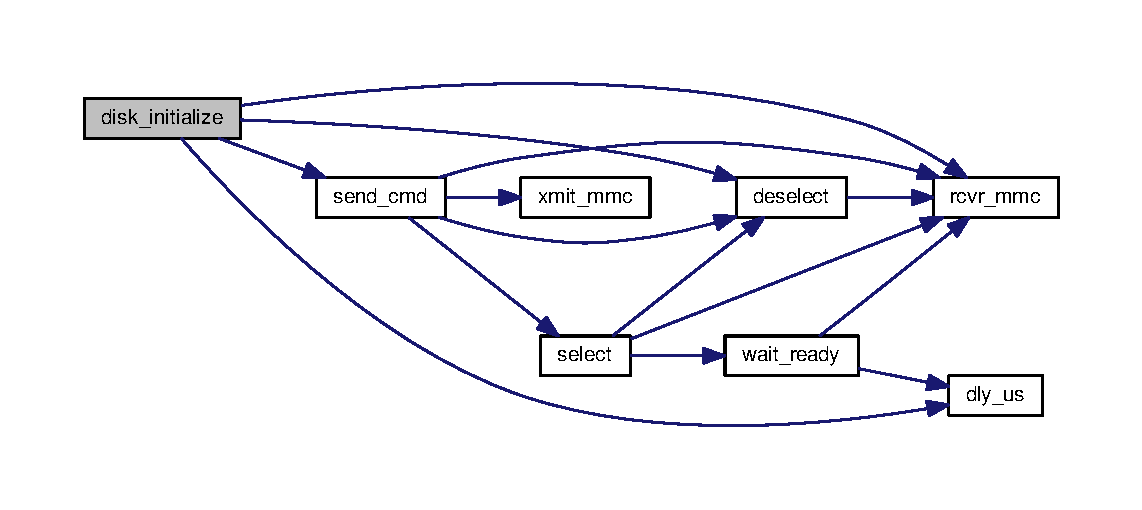
\includegraphics[width=350pt]{diskio_8h_a09cdaa6f36fa409bdf002727bff98eb1_cgraph}
\end{center}
\end{figure}


\hypertarget{diskio_8h_ab00fa450a811dbdabe3c655c1a36fab4}{\index{diskio.\-h@{diskio.\-h}!disk\-\_\-ioctl@{disk\-\_\-ioctl}}
\index{disk\-\_\-ioctl@{disk\-\_\-ioctl}!diskio.h@{diskio.\-h}}
\subsubsection[{disk\-\_\-ioctl}]{\setlength{\rightskip}{0pt plus 5cm}{\bf D\-R\-E\-S\-U\-L\-T} disk\-\_\-ioctl (
\begin{DoxyParamCaption}
\item[{{\bf B\-Y\-T\-E}}]{pdrv, }
\item[{{\bf B\-Y\-T\-E}}]{cmd, }
\item[{void $\ast$}]{buff}
\end{DoxyParamCaption}
)}}\label{diskio_8h_ab00fa450a811dbdabe3c655c1a36fab4}


References C\-M\-D9, C\-T\-R\-L\-\_\-\-S\-Y\-N\-C, deselect(), disk\-\_\-status(), G\-E\-T\-\_\-\-B\-L\-O\-C\-K\-\_\-\-S\-I\-Z\-E, G\-E\-T\-\_\-\-S\-E\-C\-T\-O\-R\-\_\-\-C\-O\-U\-N\-T, rcvr\-\_\-datablock(), R\-E\-S\-\_\-\-E\-R\-R\-O\-R, R\-E\-S\-\_\-\-N\-O\-T\-R\-D\-Y, R\-E\-S\-\_\-\-O\-K, R\-E\-S\-\_\-\-P\-A\-R\-E\-R\-R, select(), send\-\_\-cmd(), and S\-T\-A\-\_\-\-N\-O\-I\-N\-I\-T.



Referenced by chk\-\_\-mounted(), remove\-\_\-chain(), and sync\-\_\-fs().



Here is the call graph for this function\-:
\nopagebreak
\begin{figure}[H]
\begin{center}
\leavevmode
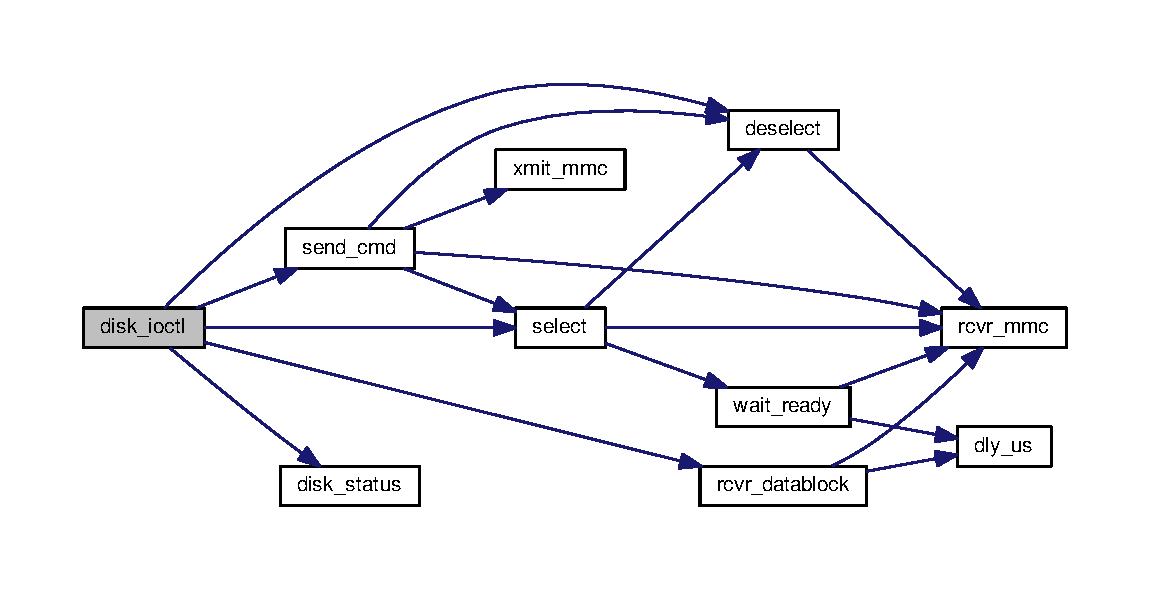
\includegraphics[width=350pt]{diskio_8h_ab00fa450a811dbdabe3c655c1a36fab4_cgraph}
\end{center}
\end{figure}


\hypertarget{diskio_8h_ac0c802f8a12fa2047b4bec7109b9293f}{\index{diskio.\-h@{diskio.\-h}!disk\-\_\-read@{disk\-\_\-read}}
\index{disk\-\_\-read@{disk\-\_\-read}!diskio.h@{diskio.\-h}}
\subsubsection[{disk\-\_\-read}]{\setlength{\rightskip}{0pt plus 5cm}{\bf D\-R\-E\-S\-U\-L\-T} disk\-\_\-read (
\begin{DoxyParamCaption}
\item[{{\bf B\-Y\-T\-E}}]{pdrv, }
\item[{{\bf B\-Y\-T\-E} $\ast$}]{buff, }
\item[{{\bf D\-W\-O\-R\-D}}]{sector, }
\item[{{\bf B\-Y\-T\-E}}]{count}
\end{DoxyParamCaption}
)}}\label{diskio_8h_ac0c802f8a12fa2047b4bec7109b9293f}


References Card\-Type, C\-M\-D12, C\-M\-D17, C\-M\-D18, C\-T\-\_\-\-B\-L\-O\-C\-K, deselect(), disk\-\_\-status(), rcvr\-\_\-datablock(), R\-E\-S\-\_\-\-E\-R\-R\-O\-R, R\-E\-S\-\_\-\-N\-O\-T\-R\-D\-Y, R\-E\-S\-\_\-\-O\-K, send\-\_\-cmd(), and S\-T\-A\-\_\-\-N\-O\-I\-N\-I\-T.



Referenced by check\-\_\-fs(), chk\-\_\-mounted(), f\-\_\-lseek(), f\-\_\-read(), f\-\_\-write(), and move\-\_\-window().



Here is the call graph for this function\-:
\nopagebreak
\begin{figure}[H]
\begin{center}
\leavevmode
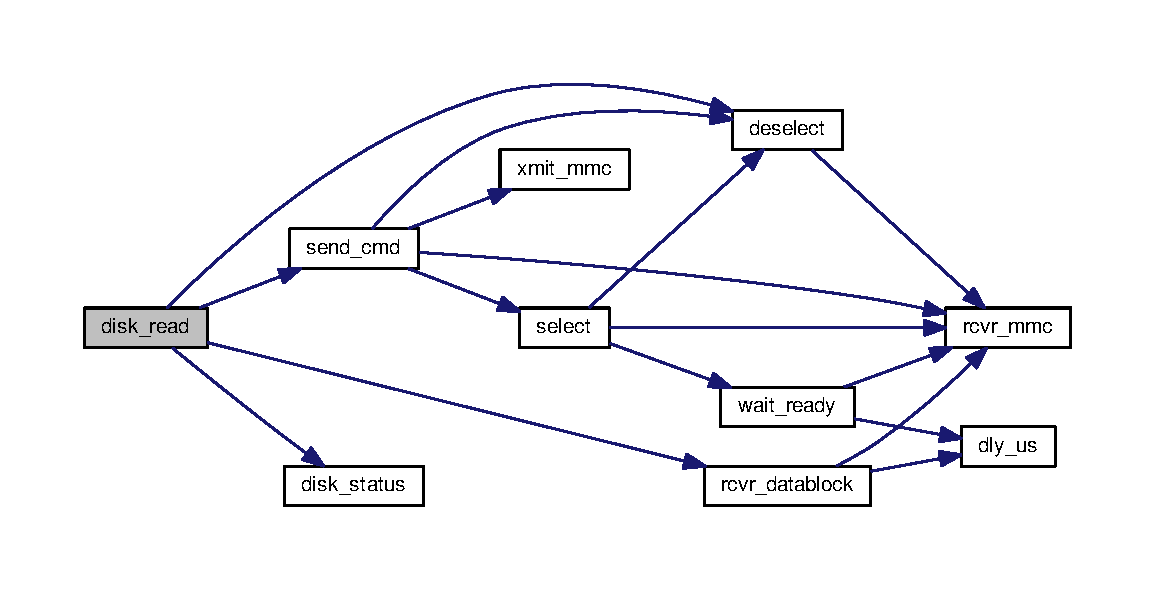
\includegraphics[width=350pt]{diskio_8h_ac0c802f8a12fa2047b4bec7109b9293f_cgraph}
\end{center}
\end{figure}


\hypertarget{diskio_8h_a8348ac5ee6d709420c02e45c111f4793}{\index{diskio.\-h@{diskio.\-h}!disk\-\_\-status@{disk\-\_\-status}}
\index{disk\-\_\-status@{disk\-\_\-status}!diskio.h@{diskio.\-h}}
\subsubsection[{disk\-\_\-status}]{\setlength{\rightskip}{0pt plus 5cm}{\bf D\-S\-T\-A\-T\-U\-S} disk\-\_\-status (
\begin{DoxyParamCaption}
\item[{{\bf B\-Y\-T\-E}}]{pdrv}
\end{DoxyParamCaption}
)}}\label{diskio_8h_a8348ac5ee6d709420c02e45c111f4793}


References S\-T\-A\-\_\-\-N\-O\-I\-N\-I\-T, and Stat.



Referenced by chk\-\_\-mounted(), disk\-\_\-ioctl(), disk\-\_\-read(), disk\-\_\-write(), and validate().

\hypertarget{diskio_8h_ac4785625f4bb82e33562079813659880}{\index{diskio.\-h@{diskio.\-h}!disk\-\_\-write@{disk\-\_\-write}}
\index{disk\-\_\-write@{disk\-\_\-write}!diskio.h@{diskio.\-h}}
\subsubsection[{disk\-\_\-write}]{\setlength{\rightskip}{0pt plus 5cm}{\bf D\-R\-E\-S\-U\-L\-T} disk\-\_\-write (
\begin{DoxyParamCaption}
\item[{{\bf B\-Y\-T\-E}}]{pdrv, }
\item[{const {\bf B\-Y\-T\-E} $\ast$}]{buff, }
\item[{{\bf D\-W\-O\-R\-D}}]{sector, }
\item[{{\bf B\-Y\-T\-E}}]{count}
\end{DoxyParamCaption}
)}}\label{diskio_8h_ac4785625f4bb82e33562079813659880}


References A\-C\-M\-D23, Card\-Type, C\-M\-D24, C\-M\-D25, C\-T\-\_\-\-B\-L\-O\-C\-K, C\-T\-\_\-\-S\-D\-C, deselect(), disk\-\_\-status(), R\-E\-S\-\_\-\-E\-R\-R\-O\-R, R\-E\-S\-\_\-\-N\-O\-T\-R\-D\-Y, R\-E\-S\-\_\-\-O\-K, send\-\_\-cmd(), S\-T\-A\-\_\-\-N\-O\-I\-N\-I\-T, and xmit\-\_\-datablock().



Referenced by f\-\_\-lseek(), f\-\_\-read(), f\-\_\-sync(), f\-\_\-write(), sync\-\_\-fs(), and sync\-\_\-window().



Here is the call graph for this function\-:
\nopagebreak
\begin{figure}[H]
\begin{center}
\leavevmode
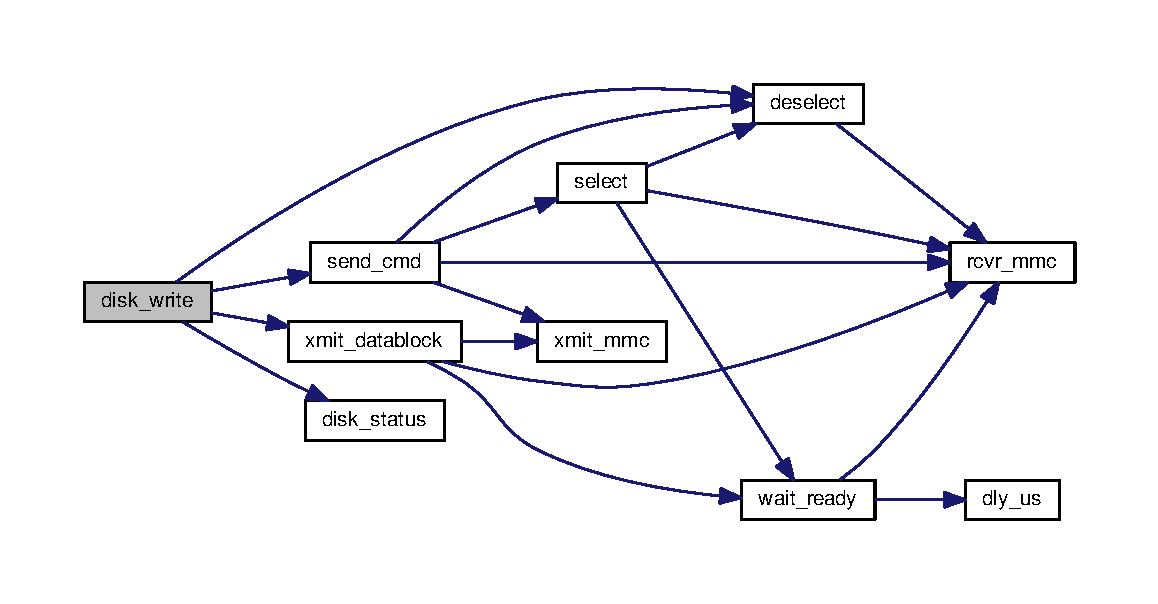
\includegraphics[width=350pt]{diskio_8h_ac4785625f4bb82e33562079813659880_cgraph}
\end{center}
\end{figure}



\hypertarget{ff_8c}{\section{sd\-\_\-card/ff.c File Reference}
\label{ff_8c}\index{sd\-\_\-card/ff.\-c@{sd\-\_\-card/ff.\-c}}
}
{\ttfamily \#include \char`\"{}ff.\-h\char`\"{}}\\*
{\ttfamily \#include \char`\"{}diskio.\-h\char`\"{}}\\*
Include dependency graph for ff.\-c\-:\nopagebreak
\begin{figure}[H]
\begin{center}
\leavevmode
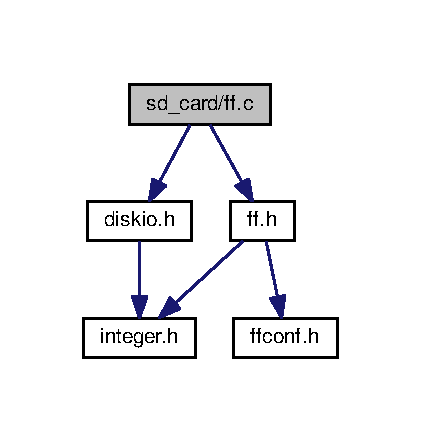
\includegraphics[width=202pt]{ff_8c__incl}
\end{center}
\end{figure}
\subsection*{Macros}
\begin{DoxyCompactItemize}
\item 
\#define \hyperlink{ff_8c_a42b5140fc5e09a53c8f4cba66dc0e6c1}{S\-S}(fs)~512\-U			/$\ast$ Fixed sector size $\ast$/
\item 
\#define \hyperlink{ff_8c_a458e336ac53f8249ed02d844469b7076}{E\-N\-T\-E\-R\-\_\-\-F\-F}(fs)
\item 
\#define \hyperlink{ff_8c_a7e653d8ca0ae09faa49cd5b7335fea84}{L\-E\-A\-V\-E\-\_\-\-F\-F}(fs, res)~return res
\item 
\#define \hyperlink{ff_8c_a41e4c46636679236568cf50b5535847f}{A\-B\-O\-R\-T}(fs, res)~\{ \hyperlink{main_8c_a8d839bbcaa5e21902d2481c87c4f359f}{fp}-\/$>$flag $\vert$= \hyperlink{ff_8h_ad3b47fe8126573b17752a9a242b76b9a}{F\-A\-\_\-\-\_\-\-E\-R\-R\-O\-R}; \hyperlink{ff_8c_a7e653d8ca0ae09faa49cd5b7335fea84}{L\-E\-A\-V\-E\-\_\-\-F\-F}(fs, res); \}
\item 
\#define \hyperlink{ff_8c_a228bfd2cabe490c8567aaf08b8b2cc14}{\-\_\-\-D\-F1\-S}~0
\item 
\#define \hyperlink{ff_8c_a4d9c368236443f6568fd60eebb809d0f}{\-\_\-\-E\-X\-C\-V\-T}
\item 
\#define \hyperlink{ff_8c_a89b2514198590e139dd064c5d534f302}{Is\-Upper}(c)~(((c)$>$='A')\&\&((c)$<$='Z'))
\item 
\#define \hyperlink{ff_8c_a4a9d454724926bd51a3aed589a97f08b}{Is\-Lower}(c)~(((c)$>$='a')\&\&((c)$<$='z'))
\item 
\#define \hyperlink{ff_8c_a65dee564f69f2ec27f25b67a348018b9}{Is\-Digit}(c)~(((c)$>$='0')\&\&((c)$<$='9'))
\item 
\#define \hyperlink{ff_8c_a58d63a832a117f179e41c7373d013dd6}{Is\-D\-B\-C\-S1}(c)~0
\item 
\#define \hyperlink{ff_8c_a66a3fa880af6078ef181656c1d7d8ef1}{Is\-D\-B\-C\-S2}(c)~0
\item 
\#define \hyperlink{ff_8c_a06c201f90533d5b49cd039c960327968}{N\-S}~11		/$\ast$ Index of name status byte in fn\mbox{[}$\,$\mbox{]} $\ast$/
\item 
\#define \hyperlink{ff_8c_ac92c92c3a3d6b9235ac98feeb00e565a}{N\-S\-\_\-\-L\-O\-S\-S}~0x01	/$\ast$ Out of 8.\-3 format $\ast$/
\item 
\#define \hyperlink{ff_8c_ae957b8d4065ea0b3eed822aec5368d29}{N\-S\-\_\-\-L\-F\-N}~0x02	/$\ast$ Force to create L\-F\-N entry $\ast$/
\item 
\#define \hyperlink{ff_8c_a5a0742bfc1d94f0c3baa5ede485048c4}{N\-S\-\_\-\-L\-A\-S\-T}~0x04	/$\ast$ Last segment $\ast$/
\item 
\#define \hyperlink{ff_8c_a4a0e89b504dece19e2e4b02c83782ca2}{N\-S\-\_\-\-B\-O\-D\-Y}~0x08	/$\ast$ Lower case flag (body) $\ast$/
\item 
\#define \hyperlink{ff_8c_a3b7fad0942e816fdb84d869c1f7a613e}{N\-S\-\_\-\-E\-X\-T}~0x10	/$\ast$ Lower case flag (ext) $\ast$/
\item 
\#define \hyperlink{ff_8c_a2db528782a021797b34bdc6e9e9de1c3}{N\-S\-\_\-\-D\-O\-T}~0x20	/$\ast$ Dot entry $\ast$/
\item 
\#define \hyperlink{ff_8c_aeec02d5ae07ede32b7d74155bf0fda15}{M\-I\-N\-\_\-\-F\-A\-T16}~4086	/$\ast$ Minimum number of clusters for F\-A\-T16 $\ast$/
\item 
\#define \hyperlink{ff_8c_a483625319f3e3bd5ac6502b46c375aed}{M\-I\-N\-\_\-\-F\-A\-T32}~65526	/$\ast$ Minimum number of clusters for F\-A\-T32 $\ast$/
\item 
\#define \hyperlink{ff_8c_a8f81669ee736efb2b2b49c7b0985472d}{B\-S\-\_\-jmp\-Boot}~0	/$\ast$ Jump instruction (3) $\ast$/
\item 
\#define \hyperlink{ff_8c_a02a76ada191ec2dc5f8af60ff3576da7}{B\-S\-\_\-\-O\-E\-M\-Name}~3	/$\ast$ O\-E\-M name (8) $\ast$/
\item 
\#define \hyperlink{ff_8c_a8551844b4eb4e15aecd8cc9aa3585fa2}{B\-P\-B\-\_\-\-Byts\-Per\-Sec}~11	/$\ast$ Sector size \mbox{[}byte\mbox{]} (2) $\ast$/
\item 
\#define \hyperlink{ff_8c_aab78e41c617a14b9540c0563d6b957fa}{B\-P\-B\-\_\-\-Sec\-Per\-Clus}~13	/$\ast$ Cluster size \mbox{[}sector\mbox{]} (1) $\ast$/
\item 
\#define \hyperlink{ff_8c_ab3ec444c8457c9bc98aa07e846f5c1b7}{B\-P\-B\-\_\-\-Rsvd\-Sec\-Cnt}~14	/$\ast$ Size of reserved area \mbox{[}sector\mbox{]} (2) $\ast$/
\item 
\#define \hyperlink{ff_8c_af44a1e8c89ec5502595f23496d24cbf1}{B\-P\-B\-\_\-\-Num\-F\-A\-Ts}~16	/$\ast$ Number of F\-A\-T copies (1) $\ast$/
\item 
\#define \hyperlink{ff_8c_aaa667f14c87c45dc128f2ab208e92f98}{B\-P\-B\-\_\-\-Root\-Ent\-Cnt}~17	/$\ast$ Number of root dir entries for F\-A\-T12/16 (2) $\ast$/
\item 
\#define \hyperlink{ff_8c_a4eb540eecde0f2df26fa8c7969341d68}{B\-P\-B\-\_\-\-Tot\-Sec16}~19	/$\ast$ Volume size \mbox{[}sector\mbox{]} (2) $\ast$/
\item 
\#define \hyperlink{ff_8c_a414e054c4b5ea3414ebefa3539e7e554}{B\-P\-B\-\_\-\-Media}~21	/$\ast$ Media descriptor (1) $\ast$/
\item 
\#define \hyperlink{ff_8c_a60a2f6efeb6a4c7cb2da1e5def6ca43b}{B\-P\-B\-\_\-\-F\-A\-T\-Sz16}~22	/$\ast$ F\-A\-T size \mbox{[}sector\mbox{]} (2) $\ast$/
\item 
\#define \hyperlink{ff_8c_ac71bb771432ea532bc47713a028ebd76}{B\-P\-B\-\_\-\-Sec\-Per\-Trk}~24	/$\ast$ Track size \mbox{[}sector\mbox{]} (2) $\ast$/
\item 
\#define \hyperlink{ff_8c_a9c03603c3be34d4c5cc1b481b0bc6774}{B\-P\-B\-\_\-\-Num\-Heads}~26	/$\ast$ Number of heads (2) $\ast$/
\item 
\#define \hyperlink{ff_8c_a449d4ed5c4c8105daf29aad9488277f7}{B\-P\-B\-\_\-\-Hidd\-Sec}~28	/$\ast$ Number of special hidden sectors (4) $\ast$/
\item 
\#define \hyperlink{ff_8c_a7723a9f0da553e8879d60909d85ccb7b}{B\-P\-B\-\_\-\-Tot\-Sec32}~32	/$\ast$ Volume size \mbox{[}sector\mbox{]} (4) $\ast$/
\item 
\#define \hyperlink{ff_8c_a0c51f7393341b839dfb241c2951f3ef4}{B\-S\-\_\-\-Drv\-Num}~36	/$\ast$ Physical drive number (2) $\ast$/
\item 
\#define \hyperlink{ff_8c_a85a92e790602efef4da3a2f141611ce8}{B\-S\-\_\-\-Boot\-Sig}~38	/$\ast$ Extended boot signature (1) $\ast$/
\item 
\#define \hyperlink{ff_8c_a383a71bda500a0fb5a37f4edd785acbf}{B\-S\-\_\-\-Vol\-I\-D}~39	/$\ast$ Volume serial number (4) $\ast$/
\item 
\#define \hyperlink{ff_8c_a28498ba4b07ff90aaa9628e81fb89d32}{B\-S\-\_\-\-Vol\-Lab}~43	/$\ast$ Volume label (8) $\ast$/
\item 
\#define \hyperlink{ff_8c_a2264848692d36c1b2499c9b6a10acf75}{B\-S\-\_\-\-Fil\-Sys\-Type}~54	/$\ast$ File system type (1) $\ast$/
\item 
\#define \hyperlink{ff_8c_a6e6340030dc29e7da2e9f92e472a763d}{B\-P\-B\-\_\-\-F\-A\-T\-Sz32}~36	/$\ast$ F\-A\-T size \mbox{[}sector\mbox{]} (4) $\ast$/
\item 
\#define \hyperlink{ff_8c_a6c832cd9e28f8e4fbbd45fdc86c7ebbb}{B\-P\-B\-\_\-\-Ext\-Flags}~40	/$\ast$ Extended flags (2) $\ast$/
\item 
\#define \hyperlink{ff_8c_a1f75a149df65028e24d43727b9ffcb9d}{B\-P\-B\-\_\-\-F\-S\-Ver}~42	/$\ast$ File system version (2) $\ast$/
\item 
\#define \hyperlink{ff_8c_a7add0104bd20083d6940d616faecd45a}{B\-P\-B\-\_\-\-Root\-Clus}~44	/$\ast$ Root dir first cluster (4) $\ast$/
\item 
\#define \hyperlink{ff_8c_a51c45669282b9ce9da5152231df9f3ac}{B\-P\-B\-\_\-\-F\-S\-Info}~48	/$\ast$ Offset of F\-S\-Info sector (2) $\ast$/
\item 
\#define \hyperlink{ff_8c_a383726fb93488d41866028b4f07c90e1}{B\-P\-B\-\_\-\-Bk\-Boot\-Sec}~50	/$\ast$ Offset of backup boot sector (2) $\ast$/
\item 
\#define \hyperlink{ff_8c_aa670c7b495f5b347c442df67b188c58f}{B\-S\-\_\-\-Drv\-Num32}~64	/$\ast$ Physical drive number (2) $\ast$/
\item 
\#define \hyperlink{ff_8c_a59c4b2f802ab4bc9319e5bd840e615b8}{B\-S\-\_\-\-Boot\-Sig32}~66	/$\ast$ Extended boot signature (1) $\ast$/
\item 
\#define \hyperlink{ff_8c_abaa3aafdcf5e83f8cb7e2bb373b13525}{B\-S\-\_\-\-Vol\-I\-D32}~67	/$\ast$ Volume serial number (4) $\ast$/
\item 
\#define \hyperlink{ff_8c_a8241a49bce313184a58617ba1ad9e84c}{B\-S\-\_\-\-Vol\-Lab32}~71	/$\ast$ Volume label (8) $\ast$/
\item 
\#define \hyperlink{ff_8c_a8d8786452966cd0ce579f2575a54a348}{B\-S\-\_\-\-Fil\-Sys\-Type32}~82	/$\ast$ File system type (1) $\ast$/
\item 
\#define \hyperlink{ff_8c_a318e58c1966aba52b90ab98dcb649883}{F\-S\-I\-\_\-\-Lead\-Sig}~0	/$\ast$ F\-S\-I\-: Leading signature (4) $\ast$/
\item 
\#define \hyperlink{ff_8c_a3bac0e6ff5907873030db1d0a7c4ebef}{F\-S\-I\-\_\-\-Struc\-Sig}~484	/$\ast$ F\-S\-I\-: Structure signature (4) $\ast$/
\item 
\#define \hyperlink{ff_8c_ab711e50459aba01b11c6b46a7cc1410b}{F\-S\-I\-\_\-\-Free\-\_\-\-Count}~488	/$\ast$ F\-S\-I\-: Number of free clusters (4) $\ast$/
\item 
\#define \hyperlink{ff_8c_a320700cedf300c9b418edf56e5e6b086}{F\-S\-I\-\_\-\-Nxt\-\_\-\-Free}~492	/$\ast$ F\-S\-I\-: Last allocated cluster (4) $\ast$/
\item 
\#define \hyperlink{ff_8c_ac3f187bf0ba891551f594af6b61f3188}{M\-B\-R\-\_\-\-Table}~446	/$\ast$ M\-B\-R\-: Partition table offset (2) $\ast$/
\item 
\#define \hyperlink{ff_8c_af133060c47366e7e557d4085d931183f}{S\-Z\-\_\-\-P\-T\-E}~16	/$\ast$ M\-B\-R\-: Size of a partition table entry $\ast$/
\item 
\#define \hyperlink{ff_8c_a74b810b3f3583c1eb54bd4305c0f261a}{B\-S\-\_\-55\-A\-A}~510	/$\ast$ Boot sector signature (2) $\ast$/
\item 
\#define \hyperlink{ff_8c_afa89348e9fc2de82ae9e12c661366b0e}{D\-I\-R\-\_\-\-Name}~0	/$\ast$ Short file name (11) $\ast$/
\item 
\#define \hyperlink{ff_8c_ad3233e40118ed66095f3c9545b788f8a}{D\-I\-R\-\_\-\-Attr}~11	/$\ast$ Attribute (1) $\ast$/
\item 
\#define \hyperlink{ff_8c_a87ee1f701c2ab941862e3ce00c1c1e9d}{D\-I\-R\-\_\-\-N\-Tres}~12	/$\ast$ N\-T flag (1) $\ast$/
\item 
\#define \hyperlink{ff_8c_a55fd459982581ae39fe3aeb242b2bc0f}{D\-I\-R\-\_\-\-Crt\-Time\-Tenth}~13	/$\ast$ Created time sub-\/second (1) $\ast$/
\item 
\#define \hyperlink{ff_8c_a47fb1881ea71d860db9b8280564cb4d5}{D\-I\-R\-\_\-\-Crt\-Time}~14	/$\ast$ Created time (2) $\ast$/
\item 
\#define \hyperlink{ff_8c_acf498617bb4c7750fd738864c3c0ab5a}{D\-I\-R\-\_\-\-Crt\-Date}~16	/$\ast$ Created date (2) $\ast$/
\item 
\#define \hyperlink{ff_8c_afa0625d73f4683df24345f51e7a43da3}{D\-I\-R\-\_\-\-Lst\-Acc\-Date}~18	/$\ast$ Last accessed date (2) $\ast$/
\item 
\#define \hyperlink{ff_8c_a0bc29c3f09e1e9c40c414f7d50d7905c}{D\-I\-R\-\_\-\-Fst\-Clus\-H\-I}~20	/$\ast$ Higher 16-\/bit of first cluster (2) $\ast$/
\item 
\#define \hyperlink{ff_8c_ab9452d336adeece2a1b0b54ab35b8a59}{D\-I\-R\-\_\-\-Wrt\-Time}~22	/$\ast$ Modified time (2) $\ast$/
\item 
\#define \hyperlink{ff_8c_abed17fa699511b09cbf64961373d63a4}{D\-I\-R\-\_\-\-Wrt\-Date}~24	/$\ast$ Modified date (2) $\ast$/
\item 
\#define \hyperlink{ff_8c_aebe0e913bff75a89d38dbcb04baf5dff}{D\-I\-R\-\_\-\-Fst\-Clus\-L\-O}~26	/$\ast$ Lower 16-\/bit of first cluster (2) $\ast$/
\item 
\#define \hyperlink{ff_8c_abfbfa613864a02a65f0bf70ead6672c7}{D\-I\-R\-\_\-\-File\-Size}~28	/$\ast$ File size (4) $\ast$/
\item 
\#define \hyperlink{ff_8c_a6c97d545619e6586b02b5d4f39f7be25}{L\-D\-I\-R\-\_\-\-Ord}~0	/$\ast$ L\-F\-N entry \hyperlink{structorder}{order} and \hyperlink{ff_8c_aff828b43518c49e1d637a822879b135d}{L\-L\-E} flag (1) $\ast$/
\item 
\#define \hyperlink{ff_8c_a28dcd75633b49e40b42a31f0cf5f5929}{L\-D\-I\-R\-\_\-\-Attr}~11	/$\ast$ L\-F\-N attribute (1) $\ast$/
\item 
\#define \hyperlink{ff_8c_acb98a052a9be81564b56854df35480a0}{L\-D\-I\-R\-\_\-\-Type}~12	/$\ast$ L\-F\-N type (1) $\ast$/
\item 
\#define \hyperlink{ff_8c_ade1d529763d2d097a6d1410956c8a84f}{L\-D\-I\-R\-\_\-\-Chksum}~13	/$\ast$ Sum of corresponding S\-F\-N entry $\ast$/
\item 
\#define \hyperlink{ff_8c_ad73024151eff6baea94e680f7928969d}{L\-D\-I\-R\-\_\-\-Fst\-Clus\-L\-O}~26	/$\ast$ Filled by zero (0) $\ast$/
\item 
\#define \hyperlink{ff_8c_ab10c2f2271dbdc132f9a6b9313fc7324}{S\-Z\-\_\-\-D\-I\-R}~32		/$\ast$ Size of a directory entry $\ast$/
\item 
\#define \hyperlink{ff_8c_aff828b43518c49e1d637a822879b135d}{L\-L\-E}~0x40	/$\ast$ Last long entry flag in L\-D\-I\-R\-\_\-\-Ord $\ast$/
\item 
\#define \hyperlink{ff_8c_af39f317ac33b961daaff4b8d8a7ec792}{D\-D\-E}~0x\-E5	/$\ast$ Deleted directory entry mark in D\-I\-R\-\_\-\-Name\mbox{[}0\mbox{]} $\ast$/
\item 
\#define \hyperlink{ff_8c_a741d6fdda5989919e0bb9811da804e56}{N\-D\-D\-E}~0x05	/$\ast$ Replacement of the character collides with D\-D\-E $\ast$/
\item 
\#define \hyperlink{ff_8c_a40aba328871d2be78bfdd74b390275db}{D\-E\-F\-\_\-\-N\-A\-M\-E\-B\-U\-F}~\hyperlink{integer_8h_a4ae1dab0fb4b072a66584546209e7d58}{B\-Y\-T\-E} sfn\mbox{[}12\mbox{]}
\item 
\#define \hyperlink{ff_8c_a966fe5792671b39db1ccf655a8c1af8d}{I\-N\-I\-T\-\_\-\-B\-U\-F}(dobj)~(dobj).fn = sfn
\item 
\#define \hyperlink{ff_8c_aba6d6942b59f11cf285bdbfb7e38f1fa}{F\-R\-E\-E\-\_\-\-B\-U\-F}()
\end{DoxyCompactItemize}
\subsection*{Functions}
\begin{DoxyCompactItemize}
\item 
static void \hyperlink{ff_8c_a8941d573d16af92c8570950d53164f30}{mem\-\_\-cpy} (void $\ast$dst, const void $\ast$src, \hyperlink{integer_8h_a36cb3b01d81ffd844bbbfb54003e06ec}{U\-I\-N\-T} cnt)
\item 
static void \hyperlink{ff_8c_a02eb5189e43056a9ddc8a59cbe89be93}{mem\-\_\-set} (void $\ast$dst, int val, \hyperlink{integer_8h_a36cb3b01d81ffd844bbbfb54003e06ec}{U\-I\-N\-T} cnt)
\item 
static int \hyperlink{ff_8c_a38b4f223d18bd4416d8bce0f07a63c01}{mem\-\_\-cmp} (const void $\ast$dst, const void $\ast$src, \hyperlink{integer_8h_a36cb3b01d81ffd844bbbfb54003e06ec}{U\-I\-N\-T} cnt)
\item 
static int \hyperlink{ff_8c_a1a60c4200d040e4f47e87dc927f23d14}{chk\-\_\-chr} (const char $\ast$str, int chr)
\item 
static \hyperlink{ff_8h_a49d0171ecbd362cda5680a0d360db44c}{F\-R\-E\-S\-U\-L\-T} \hyperlink{ff_8c_a5e18753404354b210096f9af99e31bc1}{sync\-\_\-window} (\hyperlink{structFATFS}{F\-A\-T\-F\-S} $\ast$fs)
\item 
static \hyperlink{ff_8h_a49d0171ecbd362cda5680a0d360db44c}{F\-R\-E\-S\-U\-L\-T} \hyperlink{ff_8c_af2e8986556ee6644b4bf31fa4158d735}{move\-\_\-window} (\hyperlink{structFATFS}{F\-A\-T\-F\-S} $\ast$fs, \hyperlink{integer_8h_ad342ac907eb044443153a22f964bf0af}{D\-W\-O\-R\-D} sector)
\item 
static \hyperlink{ff_8h_a49d0171ecbd362cda5680a0d360db44c}{F\-R\-E\-S\-U\-L\-T} \hyperlink{ff_8c_aec6b108298553219ebb2b960b528459d}{sync\-\_\-fs} (\hyperlink{structFATFS}{F\-A\-T\-F\-S} $\ast$fs)
\item 
\hyperlink{integer_8h_ad342ac907eb044443153a22f964bf0af}{D\-W\-O\-R\-D} \hyperlink{ff_8c_a7519abb60fe91f6aa1d17f64fbae123a}{clust2sect} (\hyperlink{structFATFS}{F\-A\-T\-F\-S} $\ast$fs, \hyperlink{integer_8h_ad342ac907eb044443153a22f964bf0af}{D\-W\-O\-R\-D} clst)
\item 
\hyperlink{integer_8h_ad342ac907eb044443153a22f964bf0af}{D\-W\-O\-R\-D} \hyperlink{ff_8c_a65611adf1626e5e08da77cd33a98dd8b}{get\-\_\-fat} (\hyperlink{structFATFS}{F\-A\-T\-F\-S} $\ast$fs, \hyperlink{integer_8h_ad342ac907eb044443153a22f964bf0af}{D\-W\-O\-R\-D} clst)
\item 
\hyperlink{ff_8h_a49d0171ecbd362cda5680a0d360db44c}{F\-R\-E\-S\-U\-L\-T} \hyperlink{ff_8c_abd4b6b071a8d728a88727051c12bc6d7}{put\-\_\-fat} (\hyperlink{structFATFS}{F\-A\-T\-F\-S} $\ast$fs, \hyperlink{integer_8h_ad342ac907eb044443153a22f964bf0af}{D\-W\-O\-R\-D} clst, \hyperlink{integer_8h_ad342ac907eb044443153a22f964bf0af}{D\-W\-O\-R\-D} val)
\item 
static \hyperlink{ff_8h_a49d0171ecbd362cda5680a0d360db44c}{F\-R\-E\-S\-U\-L\-T} \hyperlink{ff_8c_ab88651d19a5597dec220fe7538cccf23}{remove\-\_\-chain} (\hyperlink{structFATFS}{F\-A\-T\-F\-S} $\ast$fs, \hyperlink{integer_8h_ad342ac907eb044443153a22f964bf0af}{D\-W\-O\-R\-D} clst)
\item 
static \hyperlink{integer_8h_ad342ac907eb044443153a22f964bf0af}{D\-W\-O\-R\-D} \hyperlink{ff_8c_acbd0a20a17c6f9b6d536490d1cc3c5ac}{create\-\_\-chain} (\hyperlink{structFATFS}{F\-A\-T\-F\-S} $\ast$fs, \hyperlink{integer_8h_ad342ac907eb044443153a22f964bf0af}{D\-W\-O\-R\-D} clst)
\item 
static \hyperlink{ff_8h_a49d0171ecbd362cda5680a0d360db44c}{F\-R\-E\-S\-U\-L\-T} \hyperlink{ff_8c_ad173ae134b70df2fe9668a90247567ff}{dir\-\_\-sdi} (\hyperlink{structDIR}{D\-I\-R} $\ast$dj, \hyperlink{integer_8h_a197942eefa7db30960ae396d68339b97}{W\-O\-R\-D} idx)
\item 
static \hyperlink{ff_8h_a49d0171ecbd362cda5680a0d360db44c}{F\-R\-E\-S\-U\-L\-T} \hyperlink{ff_8c_aa70eb326eb0c3702ae16adf0b4dce1cc}{dir\-\_\-next} (\hyperlink{structDIR}{D\-I\-R} $\ast$dj, int stretch)
\item 
static \hyperlink{ff_8h_a49d0171ecbd362cda5680a0d360db44c}{F\-R\-E\-S\-U\-L\-T} \hyperlink{ff_8c_a42a5806b264207143a41d58a4c9ff9f1}{dir\-\_\-alloc} (\hyperlink{structDIR}{D\-I\-R} $\ast$dj, \hyperlink{integer_8h_a36cb3b01d81ffd844bbbfb54003e06ec}{U\-I\-N\-T} nent)
\item 
static \hyperlink{integer_8h_ad342ac907eb044443153a22f964bf0af}{D\-W\-O\-R\-D} \hyperlink{ff_8c_a996d46ee1f9aed650880aecb4b7eb314}{ld\-\_\-clust} (\hyperlink{structFATFS}{F\-A\-T\-F\-S} $\ast$fs, \hyperlink{integer_8h_a4ae1dab0fb4b072a66584546209e7d58}{B\-Y\-T\-E} $\ast$dir)
\item 
static void \hyperlink{ff_8c_a357e5a36452e057d68378c98cd61018c}{st\-\_\-clust} (\hyperlink{integer_8h_a4ae1dab0fb4b072a66584546209e7d58}{B\-Y\-T\-E} $\ast$dir, \hyperlink{integer_8h_ad342ac907eb044443153a22f964bf0af}{D\-W\-O\-R\-D} cl)
\item 
static \hyperlink{ff_8h_a49d0171ecbd362cda5680a0d360db44c}{F\-R\-E\-S\-U\-L\-T} \hyperlink{ff_8c_a809fe0feb8e7a864bc048cbd22cc0702}{dir\-\_\-find} (\hyperlink{structDIR}{D\-I\-R} $\ast$dj)
\item 
static \hyperlink{ff_8h_a49d0171ecbd362cda5680a0d360db44c}{F\-R\-E\-S\-U\-L\-T} \hyperlink{ff_8c_ac61cefc73baae693adfdfd86e9bd4741}{dir\-\_\-read} (\hyperlink{structDIR}{D\-I\-R} $\ast$dj, int vol)
\item 
static \hyperlink{ff_8h_a49d0171ecbd362cda5680a0d360db44c}{F\-R\-E\-S\-U\-L\-T} \hyperlink{ff_8c_aa51744cb902c0cd104d3680cc05ae8b5}{dir\-\_\-register} (\hyperlink{structDIR}{D\-I\-R} $\ast$dj)
\item 
static \hyperlink{ff_8h_a49d0171ecbd362cda5680a0d360db44c}{F\-R\-E\-S\-U\-L\-T} \hyperlink{ff_8c_a0bb6c133dec7b4fda00bce387e72e636}{create\-\_\-name} (\hyperlink{structDIR}{D\-I\-R} $\ast$dj, const \hyperlink{ff_8h_a03bdb8ce5895c7e261aadc2529637546}{T\-C\-H\-A\-R} $\ast$$\ast$path)
\item 
static \hyperlink{ff_8h_a49d0171ecbd362cda5680a0d360db44c}{F\-R\-E\-S\-U\-L\-T} \hyperlink{ff_8c_aac9a82c50bb738b3d78d4a46ffdad65d}{follow\-\_\-path} (\hyperlink{structDIR}{D\-I\-R} $\ast$dj, const \hyperlink{ff_8h_a03bdb8ce5895c7e261aadc2529637546}{T\-C\-H\-A\-R} $\ast$path)
\item 
static \hyperlink{integer_8h_a4ae1dab0fb4b072a66584546209e7d58}{B\-Y\-T\-E} \hyperlink{ff_8c_a55626c76a1556af5dc5345e2c0841a65}{check\-\_\-fs} (\hyperlink{structFATFS}{F\-A\-T\-F\-S} $\ast$fs, \hyperlink{integer_8h_ad342ac907eb044443153a22f964bf0af}{D\-W\-O\-R\-D} sect)
\item 
static \hyperlink{ff_8h_a49d0171ecbd362cda5680a0d360db44c}{F\-R\-E\-S\-U\-L\-T} \hyperlink{ff_8c_acb7ec4033afc5b9041ee9c82385552db}{chk\-\_\-mounted} (const \hyperlink{ff_8h_a03bdb8ce5895c7e261aadc2529637546}{T\-C\-H\-A\-R} $\ast$$\ast$path, \hyperlink{structFATFS}{F\-A\-T\-F\-S} $\ast$$\ast$rfs, \hyperlink{integer_8h_a4ae1dab0fb4b072a66584546209e7d58}{B\-Y\-T\-E} wmode)
\item 
static \hyperlink{ff_8h_a49d0171ecbd362cda5680a0d360db44c}{F\-R\-E\-S\-U\-L\-T} \hyperlink{ff_8c_aa7193f5b86c3996b5312043a0c26da5f}{validate} (void $\ast$obj)
\item 
\hyperlink{ff_8h_a49d0171ecbd362cda5680a0d360db44c}{F\-R\-E\-S\-U\-L\-T} \hyperlink{ff_8c_a5f9e6982ad48becf73dc39c797e8569d}{f\-\_\-mount} (\hyperlink{integer_8h_a4ae1dab0fb4b072a66584546209e7d58}{B\-Y\-T\-E} vol, \hyperlink{structFATFS}{F\-A\-T\-F\-S} $\ast$fs)
\item 
\hyperlink{ff_8h_a49d0171ecbd362cda5680a0d360db44c}{F\-R\-E\-S\-U\-L\-T} \hyperlink{ff_8c_aefdef7126128d99d0b3bd82c28e54d80}{f\-\_\-open} (\hyperlink{structFIL}{F\-I\-L} $\ast$\hyperlink{main_8c_a8d839bbcaa5e21902d2481c87c4f359f}{fp}, const \hyperlink{ff_8h_a03bdb8ce5895c7e261aadc2529637546}{T\-C\-H\-A\-R} $\ast$path, \hyperlink{integer_8h_a4ae1dab0fb4b072a66584546209e7d58}{B\-Y\-T\-E} mode)
\item 
\hyperlink{ff_8h_a49d0171ecbd362cda5680a0d360db44c}{F\-R\-E\-S\-U\-L\-T} \hyperlink{ff_8c_ac4c3dcb6869ca252888eebabe39727b3}{f\-\_\-read} (\hyperlink{structFIL}{F\-I\-L} $\ast$\hyperlink{main_8c_a8d839bbcaa5e21902d2481c87c4f359f}{fp}, void $\ast$buff, \hyperlink{integer_8h_a36cb3b01d81ffd844bbbfb54003e06ec}{U\-I\-N\-T} btr, \hyperlink{integer_8h_a36cb3b01d81ffd844bbbfb54003e06ec}{U\-I\-N\-T} $\ast$br)
\item 
\hyperlink{ff_8h_a49d0171ecbd362cda5680a0d360db44c}{F\-R\-E\-S\-U\-L\-T} \hyperlink{ff_8c_ae6a4dfae8a9e308bdb2283a37ef680f2}{f\-\_\-write} (\hyperlink{structFIL}{F\-I\-L} $\ast$\hyperlink{main_8c_a8d839bbcaa5e21902d2481c87c4f359f}{fp}, const void $\ast$buff, \hyperlink{integer_8h_a36cb3b01d81ffd844bbbfb54003e06ec}{U\-I\-N\-T} btw, \hyperlink{integer_8h_a36cb3b01d81ffd844bbbfb54003e06ec}{U\-I\-N\-T} $\ast$bw)
\item 
\hyperlink{ff_8h_a49d0171ecbd362cda5680a0d360db44c}{F\-R\-E\-S\-U\-L\-T} \hyperlink{ff_8c_ad69c7246b122ba56a134939ee0eaf847}{f\-\_\-sync} (\hyperlink{structFIL}{F\-I\-L} $\ast$\hyperlink{main_8c_a8d839bbcaa5e21902d2481c87c4f359f}{fp})
\item 
\hyperlink{ff_8h_a49d0171ecbd362cda5680a0d360db44c}{F\-R\-E\-S\-U\-L\-T} \hyperlink{ff_8c_a53882db20ef4323dcfd1874d7733ffc3}{f\-\_\-close} (\hyperlink{structFIL}{F\-I\-L} $\ast$\hyperlink{main_8c_a8d839bbcaa5e21902d2481c87c4f359f}{fp})
\item 
\hyperlink{ff_8h_a49d0171ecbd362cda5680a0d360db44c}{F\-R\-E\-S\-U\-L\-T} \hyperlink{ff_8c_a5df0ac672ada972e89ef4b003e57f964}{f\-\_\-lseek} (\hyperlink{structFIL}{F\-I\-L} $\ast$\hyperlink{main_8c_a8d839bbcaa5e21902d2481c87c4f359f}{fp}, \hyperlink{integer_8h_ad342ac907eb044443153a22f964bf0af}{D\-W\-O\-R\-D} ofs)
\item 
\hyperlink{ff_8h_a49d0171ecbd362cda5680a0d360db44c}{F\-R\-E\-S\-U\-L\-T} \hyperlink{ff_8c_a430bb7b15afe7198d15a03c34641578c}{f\-\_\-getlabel} (const \hyperlink{ff_8h_a03bdb8ce5895c7e261aadc2529637546}{T\-C\-H\-A\-R} $\ast$path, \hyperlink{ff_8h_a03bdb8ce5895c7e261aadc2529637546}{T\-C\-H\-A\-R} $\ast$label, \hyperlink{integer_8h_ad342ac907eb044443153a22f964bf0af}{D\-W\-O\-R\-D} $\ast$sn)
\item 
\hyperlink{ff_8h_a49d0171ecbd362cda5680a0d360db44c}{F\-R\-E\-S\-U\-L\-T} \hyperlink{ff_8c_aa82bca64e28bc0d656a7999dd0eadec7}{f\-\_\-setlabel} (const \hyperlink{ff_8h_a03bdb8ce5895c7e261aadc2529637546}{T\-C\-H\-A\-R} $\ast$label)
\end{DoxyCompactItemize}
\subsection*{Variables}
\begin{DoxyCompactItemize}
\item 
static \hyperlink{structFATFS}{F\-A\-T\-F\-S} $\ast$ \hyperlink{ff_8c_a3d7aad0939745576943767bf6c410eaf}{Fat\-Fs} \mbox{[}\hyperlink{ffconf_8h_a366da9a40c8ceb3103a6b72ca02b9969}{\-\_\-\-V\-O\-L\-U\-M\-E\-S}\mbox{]}
\item 
static \hyperlink{integer_8h_a197942eefa7db30960ae396d68339b97}{W\-O\-R\-D} \hyperlink{ff_8c_a0b3f41d8c416222e9b1c16e36d66e18b}{Fsid}
\item 
static const \hyperlink{integer_8h_a4ae1dab0fb4b072a66584546209e7d58}{B\-Y\-T\-E} \hyperlink{ff_8c_aded249c8b2fc2c9ca7997e028d07771b}{Ex\-Cvt} \mbox{[}$\,$\mbox{]} = \hyperlink{ff_8c_a4d9c368236443f6568fd60eebb809d0f}{\-\_\-\-E\-X\-C\-V\-T}
\end{DoxyCompactItemize}


\subsection{Macro Definition Documentation}
\hypertarget{ff_8c_a228bfd2cabe490c8567aaf08b8b2cc14}{\index{ff.\-c@{ff.\-c}!\-\_\-\-D\-F1\-S@{\-\_\-\-D\-F1\-S}}
\index{\-\_\-\-D\-F1\-S@{\-\_\-\-D\-F1\-S}!ff.c@{ff.\-c}}
\subsubsection[{\-\_\-\-D\-F1\-S}]{\setlength{\rightskip}{0pt plus 5cm}\#define \-\_\-\-D\-F1\-S~0}}\label{ff_8c_a228bfd2cabe490c8567aaf08b8b2cc14}


Referenced by create\-\_\-name(), and f\-\_\-setlabel().

\hypertarget{ff_8c_a4d9c368236443f6568fd60eebb809d0f}{\index{ff.\-c@{ff.\-c}!\-\_\-\-E\-X\-C\-V\-T@{\-\_\-\-E\-X\-C\-V\-T}}
\index{\-\_\-\-E\-X\-C\-V\-T@{\-\_\-\-E\-X\-C\-V\-T}!ff.c@{ff.\-c}}
\subsubsection[{\-\_\-\-E\-X\-C\-V\-T}]{\setlength{\rightskip}{0pt plus 5cm}\#define \-\_\-\-E\-X\-C\-V\-T}}\label{ff_8c_a4d9c368236443f6568fd60eebb809d0f}
{\bfseries Value\-:}
\begin{DoxyCode}
\{0x80,0x9A,0x90,0x41,0x8E,0x41,0x8F,0x80,0x45,0x45,0x45,0x49,0x49,0x49,0x8E,0x8F,0x90,0x92,0x92,0x4F,0x99,
      0x4F,0x55,0x55,0x59,0x99,0x9A,0x9B,0x9C,0x9D,0x9E,0x9F, \(\backslash\)
                                0x41,0x49,0x4F,0x55,0xA5,0xA5,0xA6,0xA7,0xA8,0xA9,0xAA,0xAB,0xAC,0x21,0xAE,
      0xAF,0xB0,0xB1,0xB2,0xB3,0xB4,0xB5,0xB6,0xB7,0xB8,0xB9,0xBA,0xBB,0xBC,0xBD,0xBE,0xBF, \(\backslash\)
                                0xC0,0xC1,0xC2,0xC3,0xC4,0xC5,0xC6,0xC7,0xC8,0xC9,0xCA,0xCB,0xCC,0xCD,0xCE,
      0xCF,0xD0,0xD1,0xD2,0xD3,0xD4,0xD5,0xD6,0xD7,0xD8,0xD9,0xDA,0xDB,0xDC,0xDD,0xDE,0xDF, \(\backslash\)
                                0xE0,0xE1,0xE2,0xE3,0xE4,0xE5,0xE6,0xE7,0xE8,0xE9,0xEA,0xEB,0xEC,0xED,0xEE,
      0xEF,0xF0,0xF1,0xF2,0xF3,0xF4,0xF5,0xF6,0xF7,0xF8,0xF9,0xFA,0xFB,0xFC,0xFD,0xFE,0xFF\}
\end{DoxyCode}
\hypertarget{ff_8c_a41e4c46636679236568cf50b5535847f}{\index{ff.\-c@{ff.\-c}!A\-B\-O\-R\-T@{A\-B\-O\-R\-T}}
\index{A\-B\-O\-R\-T@{A\-B\-O\-R\-T}!ff.c@{ff.\-c}}
\subsubsection[{A\-B\-O\-R\-T}]{\setlength{\rightskip}{0pt plus 5cm}\#define A\-B\-O\-R\-T(
\begin{DoxyParamCaption}
\item[{}]{fs, }
\item[{}]{res}
\end{DoxyParamCaption}
)~\{ {\bf fp}-\/$>$flag $\vert$= {\bf F\-A\-\_\-\-\_\-\-E\-R\-R\-O\-R}; {\bf L\-E\-A\-V\-E\-\_\-\-F\-F}(fs, res); \}}}\label{ff_8c_a41e4c46636679236568cf50b5535847f}


Referenced by f\-\_\-lseek(), f\-\_\-read(), and f\-\_\-write().

\hypertarget{ff_8c_a383726fb93488d41866028b4f07c90e1}{\index{ff.\-c@{ff.\-c}!B\-P\-B\-\_\-\-Bk\-Boot\-Sec@{B\-P\-B\-\_\-\-Bk\-Boot\-Sec}}
\index{B\-P\-B\-\_\-\-Bk\-Boot\-Sec@{B\-P\-B\-\_\-\-Bk\-Boot\-Sec}!ff.c@{ff.\-c}}
\subsubsection[{B\-P\-B\-\_\-\-Bk\-Boot\-Sec}]{\setlength{\rightskip}{0pt plus 5cm}\#define B\-P\-B\-\_\-\-Bk\-Boot\-Sec~50	/$\ast$ Offset of backup boot sector (2) $\ast$/}}\label{ff_8c_a383726fb93488d41866028b4f07c90e1}
\hypertarget{ff_8c_a8551844b4eb4e15aecd8cc9aa3585fa2}{\index{ff.\-c@{ff.\-c}!B\-P\-B\-\_\-\-Byts\-Per\-Sec@{B\-P\-B\-\_\-\-Byts\-Per\-Sec}}
\index{B\-P\-B\-\_\-\-Byts\-Per\-Sec@{B\-P\-B\-\_\-\-Byts\-Per\-Sec}!ff.c@{ff.\-c}}
\subsubsection[{B\-P\-B\-\_\-\-Byts\-Per\-Sec}]{\setlength{\rightskip}{0pt plus 5cm}\#define B\-P\-B\-\_\-\-Byts\-Per\-Sec~11	/$\ast$ Sector size \mbox{[}byte\mbox{]} (2) $\ast$/}}\label{ff_8c_a8551844b4eb4e15aecd8cc9aa3585fa2}


Referenced by chk\-\_\-mounted().

\hypertarget{ff_8c_a6c832cd9e28f8e4fbbd45fdc86c7ebbb}{\index{ff.\-c@{ff.\-c}!B\-P\-B\-\_\-\-Ext\-Flags@{B\-P\-B\-\_\-\-Ext\-Flags}}
\index{B\-P\-B\-\_\-\-Ext\-Flags@{B\-P\-B\-\_\-\-Ext\-Flags}!ff.c@{ff.\-c}}
\subsubsection[{B\-P\-B\-\_\-\-Ext\-Flags}]{\setlength{\rightskip}{0pt plus 5cm}\#define B\-P\-B\-\_\-\-Ext\-Flags~40	/$\ast$ Extended flags (2) $\ast$/}}\label{ff_8c_a6c832cd9e28f8e4fbbd45fdc86c7ebbb}
\hypertarget{ff_8c_a60a2f6efeb6a4c7cb2da1e5def6ca43b}{\index{ff.\-c@{ff.\-c}!B\-P\-B\-\_\-\-F\-A\-T\-Sz16@{B\-P\-B\-\_\-\-F\-A\-T\-Sz16}}
\index{B\-P\-B\-\_\-\-F\-A\-T\-Sz16@{B\-P\-B\-\_\-\-F\-A\-T\-Sz16}!ff.c@{ff.\-c}}
\subsubsection[{B\-P\-B\-\_\-\-F\-A\-T\-Sz16}]{\setlength{\rightskip}{0pt plus 5cm}\#define B\-P\-B\-\_\-\-F\-A\-T\-Sz16~22	/$\ast$ F\-A\-T size \mbox{[}sector\mbox{]} (2) $\ast$/}}\label{ff_8c_a60a2f6efeb6a4c7cb2da1e5def6ca43b}


Referenced by chk\-\_\-mounted().

\hypertarget{ff_8c_a6e6340030dc29e7da2e9f92e472a763d}{\index{ff.\-c@{ff.\-c}!B\-P\-B\-\_\-\-F\-A\-T\-Sz32@{B\-P\-B\-\_\-\-F\-A\-T\-Sz32}}
\index{B\-P\-B\-\_\-\-F\-A\-T\-Sz32@{B\-P\-B\-\_\-\-F\-A\-T\-Sz32}!ff.c@{ff.\-c}}
\subsubsection[{B\-P\-B\-\_\-\-F\-A\-T\-Sz32}]{\setlength{\rightskip}{0pt plus 5cm}\#define B\-P\-B\-\_\-\-F\-A\-T\-Sz32~36	/$\ast$ F\-A\-T size \mbox{[}sector\mbox{]} (4) $\ast$/}}\label{ff_8c_a6e6340030dc29e7da2e9f92e472a763d}


Referenced by chk\-\_\-mounted().

\hypertarget{ff_8c_a51c45669282b9ce9da5152231df9f3ac}{\index{ff.\-c@{ff.\-c}!B\-P\-B\-\_\-\-F\-S\-Info@{B\-P\-B\-\_\-\-F\-S\-Info}}
\index{B\-P\-B\-\_\-\-F\-S\-Info@{B\-P\-B\-\_\-\-F\-S\-Info}!ff.c@{ff.\-c}}
\subsubsection[{B\-P\-B\-\_\-\-F\-S\-Info}]{\setlength{\rightskip}{0pt plus 5cm}\#define B\-P\-B\-\_\-\-F\-S\-Info~48	/$\ast$ Offset of F\-S\-Info sector (2) $\ast$/}}\label{ff_8c_a51c45669282b9ce9da5152231df9f3ac}


Referenced by chk\-\_\-mounted().

\hypertarget{ff_8c_a1f75a149df65028e24d43727b9ffcb9d}{\index{ff.\-c@{ff.\-c}!B\-P\-B\-\_\-\-F\-S\-Ver@{B\-P\-B\-\_\-\-F\-S\-Ver}}
\index{B\-P\-B\-\_\-\-F\-S\-Ver@{B\-P\-B\-\_\-\-F\-S\-Ver}!ff.c@{ff.\-c}}
\subsubsection[{B\-P\-B\-\_\-\-F\-S\-Ver}]{\setlength{\rightskip}{0pt plus 5cm}\#define B\-P\-B\-\_\-\-F\-S\-Ver~42	/$\ast$ File system version (2) $\ast$/}}\label{ff_8c_a1f75a149df65028e24d43727b9ffcb9d}
\hypertarget{ff_8c_a449d4ed5c4c8105daf29aad9488277f7}{\index{ff.\-c@{ff.\-c}!B\-P\-B\-\_\-\-Hidd\-Sec@{B\-P\-B\-\_\-\-Hidd\-Sec}}
\index{B\-P\-B\-\_\-\-Hidd\-Sec@{B\-P\-B\-\_\-\-Hidd\-Sec}!ff.c@{ff.\-c}}
\subsubsection[{B\-P\-B\-\_\-\-Hidd\-Sec}]{\setlength{\rightskip}{0pt plus 5cm}\#define B\-P\-B\-\_\-\-Hidd\-Sec~28	/$\ast$ Number of special hidden sectors (4) $\ast$/}}\label{ff_8c_a449d4ed5c4c8105daf29aad9488277f7}
\hypertarget{ff_8c_a414e054c4b5ea3414ebefa3539e7e554}{\index{ff.\-c@{ff.\-c}!B\-P\-B\-\_\-\-Media@{B\-P\-B\-\_\-\-Media}}
\index{B\-P\-B\-\_\-\-Media@{B\-P\-B\-\_\-\-Media}!ff.c@{ff.\-c}}
\subsubsection[{B\-P\-B\-\_\-\-Media}]{\setlength{\rightskip}{0pt plus 5cm}\#define B\-P\-B\-\_\-\-Media~21	/$\ast$ Media descriptor (1) $\ast$/}}\label{ff_8c_a414e054c4b5ea3414ebefa3539e7e554}
\hypertarget{ff_8c_af44a1e8c89ec5502595f23496d24cbf1}{\index{ff.\-c@{ff.\-c}!B\-P\-B\-\_\-\-Num\-F\-A\-Ts@{B\-P\-B\-\_\-\-Num\-F\-A\-Ts}}
\index{B\-P\-B\-\_\-\-Num\-F\-A\-Ts@{B\-P\-B\-\_\-\-Num\-F\-A\-Ts}!ff.c@{ff.\-c}}
\subsubsection[{B\-P\-B\-\_\-\-Num\-F\-A\-Ts}]{\setlength{\rightskip}{0pt plus 5cm}\#define B\-P\-B\-\_\-\-Num\-F\-A\-Ts~16	/$\ast$ Number of F\-A\-T copies (1) $\ast$/}}\label{ff_8c_af44a1e8c89ec5502595f23496d24cbf1}


Referenced by chk\-\_\-mounted().

\hypertarget{ff_8c_a9c03603c3be34d4c5cc1b481b0bc6774}{\index{ff.\-c@{ff.\-c}!B\-P\-B\-\_\-\-Num\-Heads@{B\-P\-B\-\_\-\-Num\-Heads}}
\index{B\-P\-B\-\_\-\-Num\-Heads@{B\-P\-B\-\_\-\-Num\-Heads}!ff.c@{ff.\-c}}
\subsubsection[{B\-P\-B\-\_\-\-Num\-Heads}]{\setlength{\rightskip}{0pt plus 5cm}\#define B\-P\-B\-\_\-\-Num\-Heads~26	/$\ast$ Number of heads (2) $\ast$/}}\label{ff_8c_a9c03603c3be34d4c5cc1b481b0bc6774}
\hypertarget{ff_8c_a7add0104bd20083d6940d616faecd45a}{\index{ff.\-c@{ff.\-c}!B\-P\-B\-\_\-\-Root\-Clus@{B\-P\-B\-\_\-\-Root\-Clus}}
\index{B\-P\-B\-\_\-\-Root\-Clus@{B\-P\-B\-\_\-\-Root\-Clus}!ff.c@{ff.\-c}}
\subsubsection[{B\-P\-B\-\_\-\-Root\-Clus}]{\setlength{\rightskip}{0pt plus 5cm}\#define B\-P\-B\-\_\-\-Root\-Clus~44	/$\ast$ Root dir first cluster (4) $\ast$/}}\label{ff_8c_a7add0104bd20083d6940d616faecd45a}


Referenced by chk\-\_\-mounted().

\hypertarget{ff_8c_aaa667f14c87c45dc128f2ab208e92f98}{\index{ff.\-c@{ff.\-c}!B\-P\-B\-\_\-\-Root\-Ent\-Cnt@{B\-P\-B\-\_\-\-Root\-Ent\-Cnt}}
\index{B\-P\-B\-\_\-\-Root\-Ent\-Cnt@{B\-P\-B\-\_\-\-Root\-Ent\-Cnt}!ff.c@{ff.\-c}}
\subsubsection[{B\-P\-B\-\_\-\-Root\-Ent\-Cnt}]{\setlength{\rightskip}{0pt plus 5cm}\#define B\-P\-B\-\_\-\-Root\-Ent\-Cnt~17	/$\ast$ Number of root dir entries for F\-A\-T12/16 (2) $\ast$/}}\label{ff_8c_aaa667f14c87c45dc128f2ab208e92f98}


Referenced by chk\-\_\-mounted().

\hypertarget{ff_8c_ab3ec444c8457c9bc98aa07e846f5c1b7}{\index{ff.\-c@{ff.\-c}!B\-P\-B\-\_\-\-Rsvd\-Sec\-Cnt@{B\-P\-B\-\_\-\-Rsvd\-Sec\-Cnt}}
\index{B\-P\-B\-\_\-\-Rsvd\-Sec\-Cnt@{B\-P\-B\-\_\-\-Rsvd\-Sec\-Cnt}!ff.c@{ff.\-c}}
\subsubsection[{B\-P\-B\-\_\-\-Rsvd\-Sec\-Cnt}]{\setlength{\rightskip}{0pt plus 5cm}\#define B\-P\-B\-\_\-\-Rsvd\-Sec\-Cnt~14	/$\ast$ Size of reserved area \mbox{[}sector\mbox{]} (2) $\ast$/}}\label{ff_8c_ab3ec444c8457c9bc98aa07e846f5c1b7}


Referenced by chk\-\_\-mounted().

\hypertarget{ff_8c_aab78e41c617a14b9540c0563d6b957fa}{\index{ff.\-c@{ff.\-c}!B\-P\-B\-\_\-\-Sec\-Per\-Clus@{B\-P\-B\-\_\-\-Sec\-Per\-Clus}}
\index{B\-P\-B\-\_\-\-Sec\-Per\-Clus@{B\-P\-B\-\_\-\-Sec\-Per\-Clus}!ff.c@{ff.\-c}}
\subsubsection[{B\-P\-B\-\_\-\-Sec\-Per\-Clus}]{\setlength{\rightskip}{0pt plus 5cm}\#define B\-P\-B\-\_\-\-Sec\-Per\-Clus~13	/$\ast$ Cluster size \mbox{[}sector\mbox{]} (1) $\ast$/}}\label{ff_8c_aab78e41c617a14b9540c0563d6b957fa}


Referenced by chk\-\_\-mounted().

\hypertarget{ff_8c_ac71bb771432ea532bc47713a028ebd76}{\index{ff.\-c@{ff.\-c}!B\-P\-B\-\_\-\-Sec\-Per\-Trk@{B\-P\-B\-\_\-\-Sec\-Per\-Trk}}
\index{B\-P\-B\-\_\-\-Sec\-Per\-Trk@{B\-P\-B\-\_\-\-Sec\-Per\-Trk}!ff.c@{ff.\-c}}
\subsubsection[{B\-P\-B\-\_\-\-Sec\-Per\-Trk}]{\setlength{\rightskip}{0pt plus 5cm}\#define B\-P\-B\-\_\-\-Sec\-Per\-Trk~24	/$\ast$ Track size \mbox{[}sector\mbox{]} (2) $\ast$/}}\label{ff_8c_ac71bb771432ea532bc47713a028ebd76}
\hypertarget{ff_8c_a4eb540eecde0f2df26fa8c7969341d68}{\index{ff.\-c@{ff.\-c}!B\-P\-B\-\_\-\-Tot\-Sec16@{B\-P\-B\-\_\-\-Tot\-Sec16}}
\index{B\-P\-B\-\_\-\-Tot\-Sec16@{B\-P\-B\-\_\-\-Tot\-Sec16}!ff.c@{ff.\-c}}
\subsubsection[{B\-P\-B\-\_\-\-Tot\-Sec16}]{\setlength{\rightskip}{0pt plus 5cm}\#define B\-P\-B\-\_\-\-Tot\-Sec16~19	/$\ast$ Volume size \mbox{[}sector\mbox{]} (2) $\ast$/}}\label{ff_8c_a4eb540eecde0f2df26fa8c7969341d68}


Referenced by chk\-\_\-mounted().

\hypertarget{ff_8c_a7723a9f0da553e8879d60909d85ccb7b}{\index{ff.\-c@{ff.\-c}!B\-P\-B\-\_\-\-Tot\-Sec32@{B\-P\-B\-\_\-\-Tot\-Sec32}}
\index{B\-P\-B\-\_\-\-Tot\-Sec32@{B\-P\-B\-\_\-\-Tot\-Sec32}!ff.c@{ff.\-c}}
\subsubsection[{B\-P\-B\-\_\-\-Tot\-Sec32}]{\setlength{\rightskip}{0pt plus 5cm}\#define B\-P\-B\-\_\-\-Tot\-Sec32~32	/$\ast$ Volume size \mbox{[}sector\mbox{]} (4) $\ast$/}}\label{ff_8c_a7723a9f0da553e8879d60909d85ccb7b}


Referenced by chk\-\_\-mounted().

\hypertarget{ff_8c_a74b810b3f3583c1eb54bd4305c0f261a}{\index{ff.\-c@{ff.\-c}!B\-S\-\_\-55\-A\-A@{B\-S\-\_\-55\-A\-A}}
\index{B\-S\-\_\-55\-A\-A@{B\-S\-\_\-55\-A\-A}!ff.c@{ff.\-c}}
\subsubsection[{B\-S\-\_\-55\-A\-A}]{\setlength{\rightskip}{0pt plus 5cm}\#define B\-S\-\_\-55\-A\-A~510	/$\ast$ Boot sector signature (2) $\ast$/}}\label{ff_8c_a74b810b3f3583c1eb54bd4305c0f261a}


Referenced by check\-\_\-fs(), chk\-\_\-mounted(), and sync\-\_\-fs().

\hypertarget{ff_8c_a85a92e790602efef4da3a2f141611ce8}{\index{ff.\-c@{ff.\-c}!B\-S\-\_\-\-Boot\-Sig@{B\-S\-\_\-\-Boot\-Sig}}
\index{B\-S\-\_\-\-Boot\-Sig@{B\-S\-\_\-\-Boot\-Sig}!ff.c@{ff.\-c}}
\subsubsection[{B\-S\-\_\-\-Boot\-Sig}]{\setlength{\rightskip}{0pt plus 5cm}\#define B\-S\-\_\-\-Boot\-Sig~38	/$\ast$ Extended boot signature (1) $\ast$/}}\label{ff_8c_a85a92e790602efef4da3a2f141611ce8}
\hypertarget{ff_8c_a59c4b2f802ab4bc9319e5bd840e615b8}{\index{ff.\-c@{ff.\-c}!B\-S\-\_\-\-Boot\-Sig32@{B\-S\-\_\-\-Boot\-Sig32}}
\index{B\-S\-\_\-\-Boot\-Sig32@{B\-S\-\_\-\-Boot\-Sig32}!ff.c@{ff.\-c}}
\subsubsection[{B\-S\-\_\-\-Boot\-Sig32}]{\setlength{\rightskip}{0pt plus 5cm}\#define B\-S\-\_\-\-Boot\-Sig32~66	/$\ast$ Extended boot signature (1) $\ast$/}}\label{ff_8c_a59c4b2f802ab4bc9319e5bd840e615b8}
\hypertarget{ff_8c_a0c51f7393341b839dfb241c2951f3ef4}{\index{ff.\-c@{ff.\-c}!B\-S\-\_\-\-Drv\-Num@{B\-S\-\_\-\-Drv\-Num}}
\index{B\-S\-\_\-\-Drv\-Num@{B\-S\-\_\-\-Drv\-Num}!ff.c@{ff.\-c}}
\subsubsection[{B\-S\-\_\-\-Drv\-Num}]{\setlength{\rightskip}{0pt plus 5cm}\#define B\-S\-\_\-\-Drv\-Num~36	/$\ast$ Physical drive number (2) $\ast$/}}\label{ff_8c_a0c51f7393341b839dfb241c2951f3ef4}
\hypertarget{ff_8c_aa670c7b495f5b347c442df67b188c58f}{\index{ff.\-c@{ff.\-c}!B\-S\-\_\-\-Drv\-Num32@{B\-S\-\_\-\-Drv\-Num32}}
\index{B\-S\-\_\-\-Drv\-Num32@{B\-S\-\_\-\-Drv\-Num32}!ff.c@{ff.\-c}}
\subsubsection[{B\-S\-\_\-\-Drv\-Num32}]{\setlength{\rightskip}{0pt plus 5cm}\#define B\-S\-\_\-\-Drv\-Num32~64	/$\ast$ Physical drive number (2) $\ast$/}}\label{ff_8c_aa670c7b495f5b347c442df67b188c58f}
\hypertarget{ff_8c_a2264848692d36c1b2499c9b6a10acf75}{\index{ff.\-c@{ff.\-c}!B\-S\-\_\-\-Fil\-Sys\-Type@{B\-S\-\_\-\-Fil\-Sys\-Type}}
\index{B\-S\-\_\-\-Fil\-Sys\-Type@{B\-S\-\_\-\-Fil\-Sys\-Type}!ff.c@{ff.\-c}}
\subsubsection[{B\-S\-\_\-\-Fil\-Sys\-Type}]{\setlength{\rightskip}{0pt plus 5cm}\#define B\-S\-\_\-\-Fil\-Sys\-Type~54	/$\ast$ File system type (1) $\ast$/}}\label{ff_8c_a2264848692d36c1b2499c9b6a10acf75}


Referenced by check\-\_\-fs().

\hypertarget{ff_8c_a8d8786452966cd0ce579f2575a54a348}{\index{ff.\-c@{ff.\-c}!B\-S\-\_\-\-Fil\-Sys\-Type32@{B\-S\-\_\-\-Fil\-Sys\-Type32}}
\index{B\-S\-\_\-\-Fil\-Sys\-Type32@{B\-S\-\_\-\-Fil\-Sys\-Type32}!ff.c@{ff.\-c}}
\subsubsection[{B\-S\-\_\-\-Fil\-Sys\-Type32}]{\setlength{\rightskip}{0pt plus 5cm}\#define B\-S\-\_\-\-Fil\-Sys\-Type32~82	/$\ast$ File system type (1) $\ast$/}}\label{ff_8c_a8d8786452966cd0ce579f2575a54a348}


Referenced by check\-\_\-fs().

\hypertarget{ff_8c_a8f81669ee736efb2b2b49c7b0985472d}{\index{ff.\-c@{ff.\-c}!B\-S\-\_\-jmp\-Boot@{B\-S\-\_\-jmp\-Boot}}
\index{B\-S\-\_\-jmp\-Boot@{B\-S\-\_\-jmp\-Boot}!ff.c@{ff.\-c}}
\subsubsection[{B\-S\-\_\-jmp\-Boot}]{\setlength{\rightskip}{0pt plus 5cm}\#define B\-S\-\_\-jmp\-Boot~0	/$\ast$ Jump instruction (3) $\ast$/}}\label{ff_8c_a8f81669ee736efb2b2b49c7b0985472d}
\hypertarget{ff_8c_a02a76ada191ec2dc5f8af60ff3576da7}{\index{ff.\-c@{ff.\-c}!B\-S\-\_\-\-O\-E\-M\-Name@{B\-S\-\_\-\-O\-E\-M\-Name}}
\index{B\-S\-\_\-\-O\-E\-M\-Name@{B\-S\-\_\-\-O\-E\-M\-Name}!ff.c@{ff.\-c}}
\subsubsection[{B\-S\-\_\-\-O\-E\-M\-Name}]{\setlength{\rightskip}{0pt plus 5cm}\#define B\-S\-\_\-\-O\-E\-M\-Name~3	/$\ast$ O\-E\-M name (8) $\ast$/}}\label{ff_8c_a02a76ada191ec2dc5f8af60ff3576da7}
\hypertarget{ff_8c_a383a71bda500a0fb5a37f4edd785acbf}{\index{ff.\-c@{ff.\-c}!B\-S\-\_\-\-Vol\-I\-D@{B\-S\-\_\-\-Vol\-I\-D}}
\index{B\-S\-\_\-\-Vol\-I\-D@{B\-S\-\_\-\-Vol\-I\-D}!ff.c@{ff.\-c}}
\subsubsection[{B\-S\-\_\-\-Vol\-I\-D}]{\setlength{\rightskip}{0pt plus 5cm}\#define B\-S\-\_\-\-Vol\-I\-D~39	/$\ast$ Volume serial number (4) $\ast$/}}\label{ff_8c_a383a71bda500a0fb5a37f4edd785acbf}


Referenced by f\-\_\-getlabel().

\hypertarget{ff_8c_abaa3aafdcf5e83f8cb7e2bb373b13525}{\index{ff.\-c@{ff.\-c}!B\-S\-\_\-\-Vol\-I\-D32@{B\-S\-\_\-\-Vol\-I\-D32}}
\index{B\-S\-\_\-\-Vol\-I\-D32@{B\-S\-\_\-\-Vol\-I\-D32}!ff.c@{ff.\-c}}
\subsubsection[{B\-S\-\_\-\-Vol\-I\-D32}]{\setlength{\rightskip}{0pt plus 5cm}\#define B\-S\-\_\-\-Vol\-I\-D32~67	/$\ast$ Volume serial number (4) $\ast$/}}\label{ff_8c_abaa3aafdcf5e83f8cb7e2bb373b13525}


Referenced by f\-\_\-getlabel().

\hypertarget{ff_8c_a28498ba4b07ff90aaa9628e81fb89d32}{\index{ff.\-c@{ff.\-c}!B\-S\-\_\-\-Vol\-Lab@{B\-S\-\_\-\-Vol\-Lab}}
\index{B\-S\-\_\-\-Vol\-Lab@{B\-S\-\_\-\-Vol\-Lab}!ff.c@{ff.\-c}}
\subsubsection[{B\-S\-\_\-\-Vol\-Lab}]{\setlength{\rightskip}{0pt plus 5cm}\#define B\-S\-\_\-\-Vol\-Lab~43	/$\ast$ Volume label (8) $\ast$/}}\label{ff_8c_a28498ba4b07ff90aaa9628e81fb89d32}
\hypertarget{ff_8c_a8241a49bce313184a58617ba1ad9e84c}{\index{ff.\-c@{ff.\-c}!B\-S\-\_\-\-Vol\-Lab32@{B\-S\-\_\-\-Vol\-Lab32}}
\index{B\-S\-\_\-\-Vol\-Lab32@{B\-S\-\_\-\-Vol\-Lab32}!ff.c@{ff.\-c}}
\subsubsection[{B\-S\-\_\-\-Vol\-Lab32}]{\setlength{\rightskip}{0pt plus 5cm}\#define B\-S\-\_\-\-Vol\-Lab32~71	/$\ast$ Volume label (8) $\ast$/}}\label{ff_8c_a8241a49bce313184a58617ba1ad9e84c}
\hypertarget{ff_8c_af39f317ac33b961daaff4b8d8a7ec792}{\index{ff.\-c@{ff.\-c}!D\-D\-E@{D\-D\-E}}
\index{D\-D\-E@{D\-D\-E}!ff.c@{ff.\-c}}
\subsubsection[{D\-D\-E}]{\setlength{\rightskip}{0pt plus 5cm}\#define D\-D\-E~0x\-E5	/$\ast$ Deleted directory entry mark in D\-I\-R\-\_\-\-Name\mbox{[}0\mbox{]} $\ast$/}}\label{ff_8c_af39f317ac33b961daaff4b8d8a7ec792}


Referenced by create\-\_\-name(), dir\-\_\-alloc(), dir\-\_\-find(), dir\-\_\-read(), and f\-\_\-setlabel().

\hypertarget{ff_8c_a40aba328871d2be78bfdd74b390275db}{\index{ff.\-c@{ff.\-c}!D\-E\-F\-\_\-\-N\-A\-M\-E\-B\-U\-F@{D\-E\-F\-\_\-\-N\-A\-M\-E\-B\-U\-F}}
\index{D\-E\-F\-\_\-\-N\-A\-M\-E\-B\-U\-F@{D\-E\-F\-\_\-\-N\-A\-M\-E\-B\-U\-F}!ff.c@{ff.\-c}}
\subsubsection[{D\-E\-F\-\_\-\-N\-A\-M\-E\-B\-U\-F}]{\setlength{\rightskip}{0pt plus 5cm}\#define D\-E\-F\-\_\-\-N\-A\-M\-E\-B\-U\-F~{\bf B\-Y\-T\-E} sfn\mbox{[}12\mbox{]}}}\label{ff_8c_a40aba328871d2be78bfdd74b390275db}


Referenced by f\-\_\-open().

\hypertarget{ff_8c_ad3233e40118ed66095f3c9545b788f8a}{\index{ff.\-c@{ff.\-c}!D\-I\-R\-\_\-\-Attr@{D\-I\-R\-\_\-\-Attr}}
\index{D\-I\-R\-\_\-\-Attr@{D\-I\-R\-\_\-\-Attr}!ff.c@{ff.\-c}}
\subsubsection[{D\-I\-R\-\_\-\-Attr}]{\setlength{\rightskip}{0pt plus 5cm}\#define D\-I\-R\-\_\-\-Attr~11	/$\ast$ Attribute (1) $\ast$/}}\label{ff_8c_ad3233e40118ed66095f3c9545b788f8a}


Referenced by dir\-\_\-find(), dir\-\_\-read(), f\-\_\-open(), f\-\_\-setlabel(), f\-\_\-sync(), and follow\-\_\-path().

\hypertarget{ff_8c_acf498617bb4c7750fd738864c3c0ab5a}{\index{ff.\-c@{ff.\-c}!D\-I\-R\-\_\-\-Crt\-Date@{D\-I\-R\-\_\-\-Crt\-Date}}
\index{D\-I\-R\-\_\-\-Crt\-Date@{D\-I\-R\-\_\-\-Crt\-Date}!ff.c@{ff.\-c}}
\subsubsection[{D\-I\-R\-\_\-\-Crt\-Date}]{\setlength{\rightskip}{0pt plus 5cm}\#define D\-I\-R\-\_\-\-Crt\-Date~16	/$\ast$ Created date (2) $\ast$/}}\label{ff_8c_acf498617bb4c7750fd738864c3c0ab5a}
\hypertarget{ff_8c_a47fb1881ea71d860db9b8280564cb4d5}{\index{ff.\-c@{ff.\-c}!D\-I\-R\-\_\-\-Crt\-Time@{D\-I\-R\-\_\-\-Crt\-Time}}
\index{D\-I\-R\-\_\-\-Crt\-Time@{D\-I\-R\-\_\-\-Crt\-Time}!ff.c@{ff.\-c}}
\subsubsection[{D\-I\-R\-\_\-\-Crt\-Time}]{\setlength{\rightskip}{0pt plus 5cm}\#define D\-I\-R\-\_\-\-Crt\-Time~14	/$\ast$ Created time (2) $\ast$/}}\label{ff_8c_a47fb1881ea71d860db9b8280564cb4d5}


Referenced by f\-\_\-open().

\hypertarget{ff_8c_a55fd459982581ae39fe3aeb242b2bc0f}{\index{ff.\-c@{ff.\-c}!D\-I\-R\-\_\-\-Crt\-Time\-Tenth@{D\-I\-R\-\_\-\-Crt\-Time\-Tenth}}
\index{D\-I\-R\-\_\-\-Crt\-Time\-Tenth@{D\-I\-R\-\_\-\-Crt\-Time\-Tenth}!ff.c@{ff.\-c}}
\subsubsection[{D\-I\-R\-\_\-\-Crt\-Time\-Tenth}]{\setlength{\rightskip}{0pt plus 5cm}\#define D\-I\-R\-\_\-\-Crt\-Time\-Tenth~13	/$\ast$ Created time sub-\/second (1) $\ast$/}}\label{ff_8c_a55fd459982581ae39fe3aeb242b2bc0f}
\hypertarget{ff_8c_abfbfa613864a02a65f0bf70ead6672c7}{\index{ff.\-c@{ff.\-c}!D\-I\-R\-\_\-\-File\-Size@{D\-I\-R\-\_\-\-File\-Size}}
\index{D\-I\-R\-\_\-\-File\-Size@{D\-I\-R\-\_\-\-File\-Size}!ff.c@{ff.\-c}}
\subsubsection[{D\-I\-R\-\_\-\-File\-Size}]{\setlength{\rightskip}{0pt plus 5cm}\#define D\-I\-R\-\_\-\-File\-Size~28	/$\ast$ File size (4) $\ast$/}}\label{ff_8c_abfbfa613864a02a65f0bf70ead6672c7}


Referenced by f\-\_\-open(), and f\-\_\-sync().

\hypertarget{ff_8c_a0bc29c3f09e1e9c40c414f7d50d7905c}{\index{ff.\-c@{ff.\-c}!D\-I\-R\-\_\-\-Fst\-Clus\-H\-I@{D\-I\-R\-\_\-\-Fst\-Clus\-H\-I}}
\index{D\-I\-R\-\_\-\-Fst\-Clus\-H\-I@{D\-I\-R\-\_\-\-Fst\-Clus\-H\-I}!ff.c@{ff.\-c}}
\subsubsection[{D\-I\-R\-\_\-\-Fst\-Clus\-H\-I}]{\setlength{\rightskip}{0pt plus 5cm}\#define D\-I\-R\-\_\-\-Fst\-Clus\-H\-I~20	/$\ast$ Higher 16-\/bit of first cluster (2) $\ast$/}}\label{ff_8c_a0bc29c3f09e1e9c40c414f7d50d7905c}


Referenced by ld\-\_\-clust(), and st\-\_\-clust().

\hypertarget{ff_8c_aebe0e913bff75a89d38dbcb04baf5dff}{\index{ff.\-c@{ff.\-c}!D\-I\-R\-\_\-\-Fst\-Clus\-L\-O@{D\-I\-R\-\_\-\-Fst\-Clus\-L\-O}}
\index{D\-I\-R\-\_\-\-Fst\-Clus\-L\-O@{D\-I\-R\-\_\-\-Fst\-Clus\-L\-O}!ff.c@{ff.\-c}}
\subsubsection[{D\-I\-R\-\_\-\-Fst\-Clus\-L\-O}]{\setlength{\rightskip}{0pt plus 5cm}\#define D\-I\-R\-\_\-\-Fst\-Clus\-L\-O~26	/$\ast$ Lower 16-\/bit of first cluster (2) $\ast$/}}\label{ff_8c_aebe0e913bff75a89d38dbcb04baf5dff}


Referenced by ld\-\_\-clust(), and st\-\_\-clust().

\hypertarget{ff_8c_afa0625d73f4683df24345f51e7a43da3}{\index{ff.\-c@{ff.\-c}!D\-I\-R\-\_\-\-Lst\-Acc\-Date@{D\-I\-R\-\_\-\-Lst\-Acc\-Date}}
\index{D\-I\-R\-\_\-\-Lst\-Acc\-Date@{D\-I\-R\-\_\-\-Lst\-Acc\-Date}!ff.c@{ff.\-c}}
\subsubsection[{D\-I\-R\-\_\-\-Lst\-Acc\-Date}]{\setlength{\rightskip}{0pt plus 5cm}\#define D\-I\-R\-\_\-\-Lst\-Acc\-Date~18	/$\ast$ Last accessed date (2) $\ast$/}}\label{ff_8c_afa0625d73f4683df24345f51e7a43da3}


Referenced by f\-\_\-sync().

\hypertarget{ff_8c_afa89348e9fc2de82ae9e12c661366b0e}{\index{ff.\-c@{ff.\-c}!D\-I\-R\-\_\-\-Name@{D\-I\-R\-\_\-\-Name}}
\index{D\-I\-R\-\_\-\-Name@{D\-I\-R\-\_\-\-Name}!ff.c@{ff.\-c}}
\subsubsection[{D\-I\-R\-\_\-\-Name}]{\setlength{\rightskip}{0pt plus 5cm}\#define D\-I\-R\-\_\-\-Name~0	/$\ast$ Short file name (11) $\ast$/}}\label{ff_8c_afa89348e9fc2de82ae9e12c661366b0e}


Referenced by dir\-\_\-find(), and dir\-\_\-read().

\hypertarget{ff_8c_a87ee1f701c2ab941862e3ce00c1c1e9d}{\index{ff.\-c@{ff.\-c}!D\-I\-R\-\_\-\-N\-Tres@{D\-I\-R\-\_\-\-N\-Tres}}
\index{D\-I\-R\-\_\-\-N\-Tres@{D\-I\-R\-\_\-\-N\-Tres}!ff.c@{ff.\-c}}
\subsubsection[{D\-I\-R\-\_\-\-N\-Tres}]{\setlength{\rightskip}{0pt plus 5cm}\#define D\-I\-R\-\_\-\-N\-Tres~12	/$\ast$ N\-T flag (1) $\ast$/}}\label{ff_8c_a87ee1f701c2ab941862e3ce00c1c1e9d}


Referenced by dir\-\_\-register().

\hypertarget{ff_8c_abed17fa699511b09cbf64961373d63a4}{\index{ff.\-c@{ff.\-c}!D\-I\-R\-\_\-\-Wrt\-Date@{D\-I\-R\-\_\-\-Wrt\-Date}}
\index{D\-I\-R\-\_\-\-Wrt\-Date@{D\-I\-R\-\_\-\-Wrt\-Date}!ff.c@{ff.\-c}}
\subsubsection[{D\-I\-R\-\_\-\-Wrt\-Date}]{\setlength{\rightskip}{0pt plus 5cm}\#define D\-I\-R\-\_\-\-Wrt\-Date~24	/$\ast$ Modified date (2) $\ast$/}}\label{ff_8c_abed17fa699511b09cbf64961373d63a4}
\hypertarget{ff_8c_ab9452d336adeece2a1b0b54ab35b8a59}{\index{ff.\-c@{ff.\-c}!D\-I\-R\-\_\-\-Wrt\-Time@{D\-I\-R\-\_\-\-Wrt\-Time}}
\index{D\-I\-R\-\_\-\-Wrt\-Time@{D\-I\-R\-\_\-\-Wrt\-Time}!ff.c@{ff.\-c}}
\subsubsection[{D\-I\-R\-\_\-\-Wrt\-Time}]{\setlength{\rightskip}{0pt plus 5cm}\#define D\-I\-R\-\_\-\-Wrt\-Time~22	/$\ast$ Modified time (2) $\ast$/}}\label{ff_8c_ab9452d336adeece2a1b0b54ab35b8a59}


Referenced by f\-\_\-setlabel(), and f\-\_\-sync().

\hypertarget{ff_8c_a458e336ac53f8249ed02d844469b7076}{\index{ff.\-c@{ff.\-c}!E\-N\-T\-E\-R\-\_\-\-F\-F@{E\-N\-T\-E\-R\-\_\-\-F\-F}}
\index{E\-N\-T\-E\-R\-\_\-\-F\-F@{E\-N\-T\-E\-R\-\_\-\-F\-F}!ff.c@{ff.\-c}}
\subsubsection[{E\-N\-T\-E\-R\-\_\-\-F\-F}]{\setlength{\rightskip}{0pt plus 5cm}\#define E\-N\-T\-E\-R\-\_\-\-F\-F(
\begin{DoxyParamCaption}
\item[{}]{fs}
\end{DoxyParamCaption}
)}}\label{ff_8c_a458e336ac53f8249ed02d844469b7076}


Referenced by chk\-\_\-mounted(), and validate().

\hypertarget{ff_8c_aba6d6942b59f11cf285bdbfb7e38f1fa}{\index{ff.\-c@{ff.\-c}!F\-R\-E\-E\-\_\-\-B\-U\-F@{F\-R\-E\-E\-\_\-\-B\-U\-F}}
\index{F\-R\-E\-E\-\_\-\-B\-U\-F@{F\-R\-E\-E\-\_\-\-B\-U\-F}!ff.c@{ff.\-c}}
\subsubsection[{F\-R\-E\-E\-\_\-\-B\-U\-F}]{\setlength{\rightskip}{0pt plus 5cm}\#define F\-R\-E\-E\-\_\-\-B\-U\-F(
\begin{DoxyParamCaption}
{}
\end{DoxyParamCaption}
)}}\label{ff_8c_aba6d6942b59f11cf285bdbfb7e38f1fa}


Referenced by f\-\_\-open().

\hypertarget{ff_8c_ab711e50459aba01b11c6b46a7cc1410b}{\index{ff.\-c@{ff.\-c}!F\-S\-I\-\_\-\-Free\-\_\-\-Count@{F\-S\-I\-\_\-\-Free\-\_\-\-Count}}
\index{F\-S\-I\-\_\-\-Free\-\_\-\-Count@{F\-S\-I\-\_\-\-Free\-\_\-\-Count}!ff.c@{ff.\-c}}
\subsubsection[{F\-S\-I\-\_\-\-Free\-\_\-\-Count}]{\setlength{\rightskip}{0pt plus 5cm}\#define F\-S\-I\-\_\-\-Free\-\_\-\-Count~488	/$\ast$ F\-S\-I\-: Number of free clusters (4) $\ast$/}}\label{ff_8c_ab711e50459aba01b11c6b46a7cc1410b}


Referenced by chk\-\_\-mounted(), and sync\-\_\-fs().

\hypertarget{ff_8c_a318e58c1966aba52b90ab98dcb649883}{\index{ff.\-c@{ff.\-c}!F\-S\-I\-\_\-\-Lead\-Sig@{F\-S\-I\-\_\-\-Lead\-Sig}}
\index{F\-S\-I\-\_\-\-Lead\-Sig@{F\-S\-I\-\_\-\-Lead\-Sig}!ff.c@{ff.\-c}}
\subsubsection[{F\-S\-I\-\_\-\-Lead\-Sig}]{\setlength{\rightskip}{0pt plus 5cm}\#define F\-S\-I\-\_\-\-Lead\-Sig~0	/$\ast$ F\-S\-I\-: Leading signature (4) $\ast$/}}\label{ff_8c_a318e58c1966aba52b90ab98dcb649883}


Referenced by chk\-\_\-mounted(), and sync\-\_\-fs().

\hypertarget{ff_8c_a320700cedf300c9b418edf56e5e6b086}{\index{ff.\-c@{ff.\-c}!F\-S\-I\-\_\-\-Nxt\-\_\-\-Free@{F\-S\-I\-\_\-\-Nxt\-\_\-\-Free}}
\index{F\-S\-I\-\_\-\-Nxt\-\_\-\-Free@{F\-S\-I\-\_\-\-Nxt\-\_\-\-Free}!ff.c@{ff.\-c}}
\subsubsection[{F\-S\-I\-\_\-\-Nxt\-\_\-\-Free}]{\setlength{\rightskip}{0pt plus 5cm}\#define F\-S\-I\-\_\-\-Nxt\-\_\-\-Free~492	/$\ast$ F\-S\-I\-: Last allocated cluster (4) $\ast$/}}\label{ff_8c_a320700cedf300c9b418edf56e5e6b086}


Referenced by chk\-\_\-mounted(), and sync\-\_\-fs().

\hypertarget{ff_8c_a3bac0e6ff5907873030db1d0a7c4ebef}{\index{ff.\-c@{ff.\-c}!F\-S\-I\-\_\-\-Struc\-Sig@{F\-S\-I\-\_\-\-Struc\-Sig}}
\index{F\-S\-I\-\_\-\-Struc\-Sig@{F\-S\-I\-\_\-\-Struc\-Sig}!ff.c@{ff.\-c}}
\subsubsection[{F\-S\-I\-\_\-\-Struc\-Sig}]{\setlength{\rightskip}{0pt plus 5cm}\#define F\-S\-I\-\_\-\-Struc\-Sig~484	/$\ast$ F\-S\-I\-: Structure signature (4) $\ast$/}}\label{ff_8c_a3bac0e6ff5907873030db1d0a7c4ebef}


Referenced by chk\-\_\-mounted(), and sync\-\_\-fs().

\hypertarget{ff_8c_a966fe5792671b39db1ccf655a8c1af8d}{\index{ff.\-c@{ff.\-c}!I\-N\-I\-T\-\_\-\-B\-U\-F@{I\-N\-I\-T\-\_\-\-B\-U\-F}}
\index{I\-N\-I\-T\-\_\-\-B\-U\-F@{I\-N\-I\-T\-\_\-\-B\-U\-F}!ff.c@{ff.\-c}}
\subsubsection[{I\-N\-I\-T\-\_\-\-B\-U\-F}]{\setlength{\rightskip}{0pt plus 5cm}\#define I\-N\-I\-T\-\_\-\-B\-U\-F(
\begin{DoxyParamCaption}
\item[{}]{dobj}
\end{DoxyParamCaption}
)~(dobj).fn = sfn}}\label{ff_8c_a966fe5792671b39db1ccf655a8c1af8d}


Referenced by f\-\_\-open().

\hypertarget{ff_8c_a58d63a832a117f179e41c7373d013dd6}{\index{ff.\-c@{ff.\-c}!Is\-D\-B\-C\-S1@{Is\-D\-B\-C\-S1}}
\index{Is\-D\-B\-C\-S1@{Is\-D\-B\-C\-S1}!ff.c@{ff.\-c}}
\subsubsection[{Is\-D\-B\-C\-S1}]{\setlength{\rightskip}{0pt plus 5cm}\#define Is\-D\-B\-C\-S1(
\begin{DoxyParamCaption}
\item[{}]{c}
\end{DoxyParamCaption}
)~0}}\label{ff_8c_a58d63a832a117f179e41c7373d013dd6}


Referenced by create\-\_\-name(), f\-\_\-getlabel(), and f\-\_\-setlabel().

\hypertarget{ff_8c_a66a3fa880af6078ef181656c1d7d8ef1}{\index{ff.\-c@{ff.\-c}!Is\-D\-B\-C\-S2@{Is\-D\-B\-C\-S2}}
\index{Is\-D\-B\-C\-S2@{Is\-D\-B\-C\-S2}!ff.c@{ff.\-c}}
\subsubsection[{Is\-D\-B\-C\-S2}]{\setlength{\rightskip}{0pt plus 5cm}\#define Is\-D\-B\-C\-S2(
\begin{DoxyParamCaption}
\item[{}]{c}
\end{DoxyParamCaption}
)~0}}\label{ff_8c_a66a3fa880af6078ef181656c1d7d8ef1}


Referenced by create\-\_\-name(), f\-\_\-getlabel(), and f\-\_\-setlabel().

\hypertarget{ff_8c_a65dee564f69f2ec27f25b67a348018b9}{\index{ff.\-c@{ff.\-c}!Is\-Digit@{Is\-Digit}}
\index{Is\-Digit@{Is\-Digit}!ff.c@{ff.\-c}}
\subsubsection[{Is\-Digit}]{\setlength{\rightskip}{0pt plus 5cm}\#define Is\-Digit(
\begin{DoxyParamCaption}
\item[{}]{c}
\end{DoxyParamCaption}
)~(((c)$>$='0')\&\&((c)$<$='9'))}}\label{ff_8c_a65dee564f69f2ec27f25b67a348018b9}
\hypertarget{ff_8c_a4a9d454724926bd51a3aed589a97f08b}{\index{ff.\-c@{ff.\-c}!Is\-Lower@{Is\-Lower}}
\index{Is\-Lower@{Is\-Lower}!ff.c@{ff.\-c}}
\subsubsection[{Is\-Lower}]{\setlength{\rightskip}{0pt plus 5cm}\#define Is\-Lower(
\begin{DoxyParamCaption}
\item[{}]{c}
\end{DoxyParamCaption}
)~(((c)$>$='a')\&\&((c)$<$='z'))}}\label{ff_8c_a4a9d454724926bd51a3aed589a97f08b}


Referenced by create\-\_\-name(), and f\-\_\-setlabel().

\hypertarget{ff_8c_a89b2514198590e139dd064c5d534f302}{\index{ff.\-c@{ff.\-c}!Is\-Upper@{Is\-Upper}}
\index{Is\-Upper@{Is\-Upper}!ff.c@{ff.\-c}}
\subsubsection[{Is\-Upper}]{\setlength{\rightskip}{0pt plus 5cm}\#define Is\-Upper(
\begin{DoxyParamCaption}
\item[{}]{c}
\end{DoxyParamCaption}
)~(((c)$>$='A')\&\&((c)$<$='Z'))}}\label{ff_8c_a89b2514198590e139dd064c5d534f302}


Referenced by create\-\_\-name().

\hypertarget{ff_8c_a28dcd75633b49e40b42a31f0cf5f5929}{\index{ff.\-c@{ff.\-c}!L\-D\-I\-R\-\_\-\-Attr@{L\-D\-I\-R\-\_\-\-Attr}}
\index{L\-D\-I\-R\-\_\-\-Attr@{L\-D\-I\-R\-\_\-\-Attr}!ff.c@{ff.\-c}}
\subsubsection[{L\-D\-I\-R\-\_\-\-Attr}]{\setlength{\rightskip}{0pt plus 5cm}\#define L\-D\-I\-R\-\_\-\-Attr~11	/$\ast$ L\-F\-N attribute (1) $\ast$/}}\label{ff_8c_a28dcd75633b49e40b42a31f0cf5f5929}
\hypertarget{ff_8c_ade1d529763d2d097a6d1410956c8a84f}{\index{ff.\-c@{ff.\-c}!L\-D\-I\-R\-\_\-\-Chksum@{L\-D\-I\-R\-\_\-\-Chksum}}
\index{L\-D\-I\-R\-\_\-\-Chksum@{L\-D\-I\-R\-\_\-\-Chksum}!ff.c@{ff.\-c}}
\subsubsection[{L\-D\-I\-R\-\_\-\-Chksum}]{\setlength{\rightskip}{0pt plus 5cm}\#define L\-D\-I\-R\-\_\-\-Chksum~13	/$\ast$ Sum of corresponding S\-F\-N entry $\ast$/}}\label{ff_8c_ade1d529763d2d097a6d1410956c8a84f}


Referenced by dir\-\_\-find(), and dir\-\_\-read().

\hypertarget{ff_8c_ad73024151eff6baea94e680f7928969d}{\index{ff.\-c@{ff.\-c}!L\-D\-I\-R\-\_\-\-Fst\-Clus\-L\-O@{L\-D\-I\-R\-\_\-\-Fst\-Clus\-L\-O}}
\index{L\-D\-I\-R\-\_\-\-Fst\-Clus\-L\-O@{L\-D\-I\-R\-\_\-\-Fst\-Clus\-L\-O}!ff.c@{ff.\-c}}
\subsubsection[{L\-D\-I\-R\-\_\-\-Fst\-Clus\-L\-O}]{\setlength{\rightskip}{0pt plus 5cm}\#define L\-D\-I\-R\-\_\-\-Fst\-Clus\-L\-O~26	/$\ast$ Filled by zero (0) $\ast$/}}\label{ff_8c_ad73024151eff6baea94e680f7928969d}
\hypertarget{ff_8c_a6c97d545619e6586b02b5d4f39f7be25}{\index{ff.\-c@{ff.\-c}!L\-D\-I\-R\-\_\-\-Ord@{L\-D\-I\-R\-\_\-\-Ord}}
\index{L\-D\-I\-R\-\_\-\-Ord@{L\-D\-I\-R\-\_\-\-Ord}!ff.c@{ff.\-c}}
\subsubsection[{L\-D\-I\-R\-\_\-\-Ord}]{\setlength{\rightskip}{0pt plus 5cm}\#define L\-D\-I\-R\-\_\-\-Ord~0	/$\ast$ L\-F\-N entry {\bf order} and {\bf L\-L\-E} flag (1) $\ast$/}}\label{ff_8c_a6c97d545619e6586b02b5d4f39f7be25}
\hypertarget{ff_8c_acb98a052a9be81564b56854df35480a0}{\index{ff.\-c@{ff.\-c}!L\-D\-I\-R\-\_\-\-Type@{L\-D\-I\-R\-\_\-\-Type}}
\index{L\-D\-I\-R\-\_\-\-Type@{L\-D\-I\-R\-\_\-\-Type}!ff.c@{ff.\-c}}
\subsubsection[{L\-D\-I\-R\-\_\-\-Type}]{\setlength{\rightskip}{0pt plus 5cm}\#define L\-D\-I\-R\-\_\-\-Type~12	/$\ast$ L\-F\-N type (1) $\ast$/}}\label{ff_8c_acb98a052a9be81564b56854df35480a0}
\hypertarget{ff_8c_a7e653d8ca0ae09faa49cd5b7335fea84}{\index{ff.\-c@{ff.\-c}!L\-E\-A\-V\-E\-\_\-\-F\-F@{L\-E\-A\-V\-E\-\_\-\-F\-F}}
\index{L\-E\-A\-V\-E\-\_\-\-F\-F@{L\-E\-A\-V\-E\-\_\-\-F\-F}!ff.c@{ff.\-c}}
\subsubsection[{L\-E\-A\-V\-E\-\_\-\-F\-F}]{\setlength{\rightskip}{0pt plus 5cm}\#define L\-E\-A\-V\-E\-\_\-\-F\-F(
\begin{DoxyParamCaption}
\item[{}]{fs, }
\item[{}]{res}
\end{DoxyParamCaption}
)~return res}}\label{ff_8c_a7e653d8ca0ae09faa49cd5b7335fea84}


Referenced by f\-\_\-close(), f\-\_\-getlabel(), f\-\_\-lseek(), f\-\_\-open(), f\-\_\-read(), f\-\_\-setlabel(), f\-\_\-sync(), and f\-\_\-write().

\hypertarget{ff_8c_aff828b43518c49e1d637a822879b135d}{\index{ff.\-c@{ff.\-c}!L\-L\-E@{L\-L\-E}}
\index{L\-L\-E@{L\-L\-E}!ff.c@{ff.\-c}}
\subsubsection[{L\-L\-E}]{\setlength{\rightskip}{0pt plus 5cm}\#define L\-L\-E~0x40	/$\ast$ Last long entry flag in L\-D\-I\-R\-\_\-\-Ord $\ast$/}}\label{ff_8c_aff828b43518c49e1d637a822879b135d}
\hypertarget{ff_8c_ac3f187bf0ba891551f594af6b61f3188}{\index{ff.\-c@{ff.\-c}!M\-B\-R\-\_\-\-Table@{M\-B\-R\-\_\-\-Table}}
\index{M\-B\-R\-\_\-\-Table@{M\-B\-R\-\_\-\-Table}!ff.c@{ff.\-c}}
\subsubsection[{M\-B\-R\-\_\-\-Table}]{\setlength{\rightskip}{0pt plus 5cm}\#define M\-B\-R\-\_\-\-Table~446	/$\ast$ M\-B\-R\-: Partition table offset (2) $\ast$/}}\label{ff_8c_ac3f187bf0ba891551f594af6b61f3188}


Referenced by chk\-\_\-mounted().

\hypertarget{ff_8c_aeec02d5ae07ede32b7d74155bf0fda15}{\index{ff.\-c@{ff.\-c}!M\-I\-N\-\_\-\-F\-A\-T16@{M\-I\-N\-\_\-\-F\-A\-T16}}
\index{M\-I\-N\-\_\-\-F\-A\-T16@{M\-I\-N\-\_\-\-F\-A\-T16}!ff.c@{ff.\-c}}
\subsubsection[{M\-I\-N\-\_\-\-F\-A\-T16}]{\setlength{\rightskip}{0pt plus 5cm}\#define M\-I\-N\-\_\-\-F\-A\-T16~4086	/$\ast$ Minimum number of clusters for F\-A\-T16 $\ast$/}}\label{ff_8c_aeec02d5ae07ede32b7d74155bf0fda15}


Referenced by chk\-\_\-mounted().

\hypertarget{ff_8c_a483625319f3e3bd5ac6502b46c375aed}{\index{ff.\-c@{ff.\-c}!M\-I\-N\-\_\-\-F\-A\-T32@{M\-I\-N\-\_\-\-F\-A\-T32}}
\index{M\-I\-N\-\_\-\-F\-A\-T32@{M\-I\-N\-\_\-\-F\-A\-T32}!ff.c@{ff.\-c}}
\subsubsection[{M\-I\-N\-\_\-\-F\-A\-T32}]{\setlength{\rightskip}{0pt plus 5cm}\#define M\-I\-N\-\_\-\-F\-A\-T32~65526	/$\ast$ Minimum number of clusters for F\-A\-T32 $\ast$/}}\label{ff_8c_a483625319f3e3bd5ac6502b46c375aed}


Referenced by chk\-\_\-mounted().

\hypertarget{ff_8c_a741d6fdda5989919e0bb9811da804e56}{\index{ff.\-c@{ff.\-c}!N\-D\-D\-E@{N\-D\-D\-E}}
\index{N\-D\-D\-E@{N\-D\-D\-E}!ff.c@{ff.\-c}}
\subsubsection[{N\-D\-D\-E}]{\setlength{\rightskip}{0pt plus 5cm}\#define N\-D\-D\-E~0x05	/$\ast$ Replacement of the character collides with D\-D\-E $\ast$/}}\label{ff_8c_a741d6fdda5989919e0bb9811da804e56}


Referenced by create\-\_\-name().

\hypertarget{ff_8c_a06c201f90533d5b49cd039c960327968}{\index{ff.\-c@{ff.\-c}!N\-S@{N\-S}}
\index{N\-S@{N\-S}!ff.c@{ff.\-c}}
\subsubsection[{N\-S}]{\setlength{\rightskip}{0pt plus 5cm}\#define N\-S~11		/$\ast$ Index of name status byte in fn\mbox{[}$\,$\mbox{]} $\ast$/}}\label{ff_8c_a06c201f90533d5b49cd039c960327968}


Referenced by create\-\_\-name(), dir\-\_\-find(), dir\-\_\-register(), and follow\-\_\-path().

\hypertarget{ff_8c_a4a0e89b504dece19e2e4b02c83782ca2}{\index{ff.\-c@{ff.\-c}!N\-S\-\_\-\-B\-O\-D\-Y@{N\-S\-\_\-\-B\-O\-D\-Y}}
\index{N\-S\-\_\-\-B\-O\-D\-Y@{N\-S\-\_\-\-B\-O\-D\-Y}!ff.c@{ff.\-c}}
\subsubsection[{N\-S\-\_\-\-B\-O\-D\-Y}]{\setlength{\rightskip}{0pt plus 5cm}\#define N\-S\-\_\-\-B\-O\-D\-Y~0x08	/$\ast$ Lower case flag (body) $\ast$/}}\label{ff_8c_a4a0e89b504dece19e2e4b02c83782ca2}


Referenced by create\-\_\-name(), and dir\-\_\-register().

\hypertarget{ff_8c_a2db528782a021797b34bdc6e9e9de1c3}{\index{ff.\-c@{ff.\-c}!N\-S\-\_\-\-D\-O\-T@{N\-S\-\_\-\-D\-O\-T}}
\index{N\-S\-\_\-\-D\-O\-T@{N\-S\-\_\-\-D\-O\-T}!ff.c@{ff.\-c}}
\subsubsection[{N\-S\-\_\-\-D\-O\-T}]{\setlength{\rightskip}{0pt plus 5cm}\#define N\-S\-\_\-\-D\-O\-T~0x20	/$\ast$ Dot entry $\ast$/}}\label{ff_8c_a2db528782a021797b34bdc6e9e9de1c3}


Referenced by create\-\_\-name(), dir\-\_\-register(), and follow\-\_\-path().

\hypertarget{ff_8c_a3b7fad0942e816fdb84d869c1f7a613e}{\index{ff.\-c@{ff.\-c}!N\-S\-\_\-\-E\-X\-T@{N\-S\-\_\-\-E\-X\-T}}
\index{N\-S\-\_\-\-E\-X\-T@{N\-S\-\_\-\-E\-X\-T}!ff.c@{ff.\-c}}
\subsubsection[{N\-S\-\_\-\-E\-X\-T}]{\setlength{\rightskip}{0pt plus 5cm}\#define N\-S\-\_\-\-E\-X\-T~0x10	/$\ast$ Lower case flag (ext) $\ast$/}}\label{ff_8c_a3b7fad0942e816fdb84d869c1f7a613e}


Referenced by create\-\_\-name(), and dir\-\_\-register().

\hypertarget{ff_8c_a5a0742bfc1d94f0c3baa5ede485048c4}{\index{ff.\-c@{ff.\-c}!N\-S\-\_\-\-L\-A\-S\-T@{N\-S\-\_\-\-L\-A\-S\-T}}
\index{N\-S\-\_\-\-L\-A\-S\-T@{N\-S\-\_\-\-L\-A\-S\-T}!ff.c@{ff.\-c}}
\subsubsection[{N\-S\-\_\-\-L\-A\-S\-T}]{\setlength{\rightskip}{0pt plus 5cm}\#define N\-S\-\_\-\-L\-A\-S\-T~0x04	/$\ast$ Last segment $\ast$/}}\label{ff_8c_a5a0742bfc1d94f0c3baa5ede485048c4}


Referenced by create\-\_\-name(), and follow\-\_\-path().

\hypertarget{ff_8c_ae957b8d4065ea0b3eed822aec5368d29}{\index{ff.\-c@{ff.\-c}!N\-S\-\_\-\-L\-F\-N@{N\-S\-\_\-\-L\-F\-N}}
\index{N\-S\-\_\-\-L\-F\-N@{N\-S\-\_\-\-L\-F\-N}!ff.c@{ff.\-c}}
\subsubsection[{N\-S\-\_\-\-L\-F\-N}]{\setlength{\rightskip}{0pt plus 5cm}\#define N\-S\-\_\-\-L\-F\-N~0x02	/$\ast$ Force to create L\-F\-N entry $\ast$/}}\label{ff_8c_ae957b8d4065ea0b3eed822aec5368d29}


Referenced by create\-\_\-name(), and dir\-\_\-register().

\hypertarget{ff_8c_ac92c92c3a3d6b9235ac98feeb00e565a}{\index{ff.\-c@{ff.\-c}!N\-S\-\_\-\-L\-O\-S\-S@{N\-S\-\_\-\-L\-O\-S\-S}}
\index{N\-S\-\_\-\-L\-O\-S\-S@{N\-S\-\_\-\-L\-O\-S\-S}!ff.c@{ff.\-c}}
\subsubsection[{N\-S\-\_\-\-L\-O\-S\-S}]{\setlength{\rightskip}{0pt plus 5cm}\#define N\-S\-\_\-\-L\-O\-S\-S~0x01	/$\ast$ Out of 8.\-3 format $\ast$/}}\label{ff_8c_ac92c92c3a3d6b9235ac98feeb00e565a}


Referenced by create\-\_\-name(), dir\-\_\-find(), and dir\-\_\-register().

\hypertarget{ff_8c_a42b5140fc5e09a53c8f4cba66dc0e6c1}{\index{ff.\-c@{ff.\-c}!S\-S@{S\-S}}
\index{S\-S@{S\-S}!ff.c@{ff.\-c}}
\subsubsection[{S\-S}]{\setlength{\rightskip}{0pt plus 5cm}\#define S\-S(
\begin{DoxyParamCaption}
\item[{}]{fs}
\end{DoxyParamCaption}
)~512\-U			/$\ast$ Fixed sector size $\ast$/}}\label{ff_8c_a42b5140fc5e09a53c8f4cba66dc0e6c1}


Referenced by chk\-\_\-mounted(), dir\-\_\-next(), dir\-\_\-sdi(), f\-\_\-lseek(), f\-\_\-read(), f\-\_\-write(), get\-\_\-fat(), and put\-\_\-fat().

\hypertarget{ff_8c_ab10c2f2271dbdc132f9a6b9313fc7324}{\index{ff.\-c@{ff.\-c}!S\-Z\-\_\-\-D\-I\-R@{S\-Z\-\_\-\-D\-I\-R}}
\index{S\-Z\-\_\-\-D\-I\-R@{S\-Z\-\_\-\-D\-I\-R}!ff.c@{ff.\-c}}
\subsubsection[{S\-Z\-\_\-\-D\-I\-R}]{\setlength{\rightskip}{0pt plus 5cm}\#define S\-Z\-\_\-\-D\-I\-R~32		/$\ast$ Size of a directory entry $\ast$/}}\label{ff_8c_ab10c2f2271dbdc132f9a6b9313fc7324}


Referenced by chk\-\_\-mounted(), dir\-\_\-next(), dir\-\_\-register(), dir\-\_\-sdi(), and f\-\_\-setlabel().

\hypertarget{ff_8c_af133060c47366e7e557d4085d931183f}{\index{ff.\-c@{ff.\-c}!S\-Z\-\_\-\-P\-T\-E@{S\-Z\-\_\-\-P\-T\-E}}
\index{S\-Z\-\_\-\-P\-T\-E@{S\-Z\-\_\-\-P\-T\-E}!ff.c@{ff.\-c}}
\subsubsection[{S\-Z\-\_\-\-P\-T\-E}]{\setlength{\rightskip}{0pt plus 5cm}\#define S\-Z\-\_\-\-P\-T\-E~16	/$\ast$ M\-B\-R\-: Size of a partition table entry $\ast$/}}\label{ff_8c_af133060c47366e7e557d4085d931183f}


Referenced by chk\-\_\-mounted().



\subsection{Function Documentation}
\hypertarget{ff_8c_a55626c76a1556af5dc5345e2c0841a65}{\index{ff.\-c@{ff.\-c}!check\-\_\-fs@{check\-\_\-fs}}
\index{check\-\_\-fs@{check\-\_\-fs}!ff.c@{ff.\-c}}
\subsubsection[{check\-\_\-fs}]{\setlength{\rightskip}{0pt plus 5cm}static {\bf B\-Y\-T\-E} check\-\_\-fs (
\begin{DoxyParamCaption}
\item[{{\bf F\-A\-T\-F\-S} $\ast$}]{fs, }
\item[{{\bf D\-W\-O\-R\-D}}]{sect}
\end{DoxyParamCaption}
)\hspace{0.3cm}{\ttfamily [static]}}}\label{ff_8c_a55626c76a1556af5dc5345e2c0841a65}


References B\-S\-\_\-55\-A\-A, B\-S\-\_\-\-Fil\-Sys\-Type, B\-S\-\_\-\-Fil\-Sys\-Type32, disk\-\_\-read(), F\-A\-T\-F\-S\-::drv, L\-D\-\_\-\-D\-W\-O\-R\-D, L\-D\-\_\-\-W\-O\-R\-D, R\-E\-S\-\_\-\-O\-K, and F\-A\-T\-F\-S\-::win.



Referenced by chk\-\_\-mounted().



Here is the call graph for this function\-:
\nopagebreak
\begin{figure}[H]
\begin{center}
\leavevmode
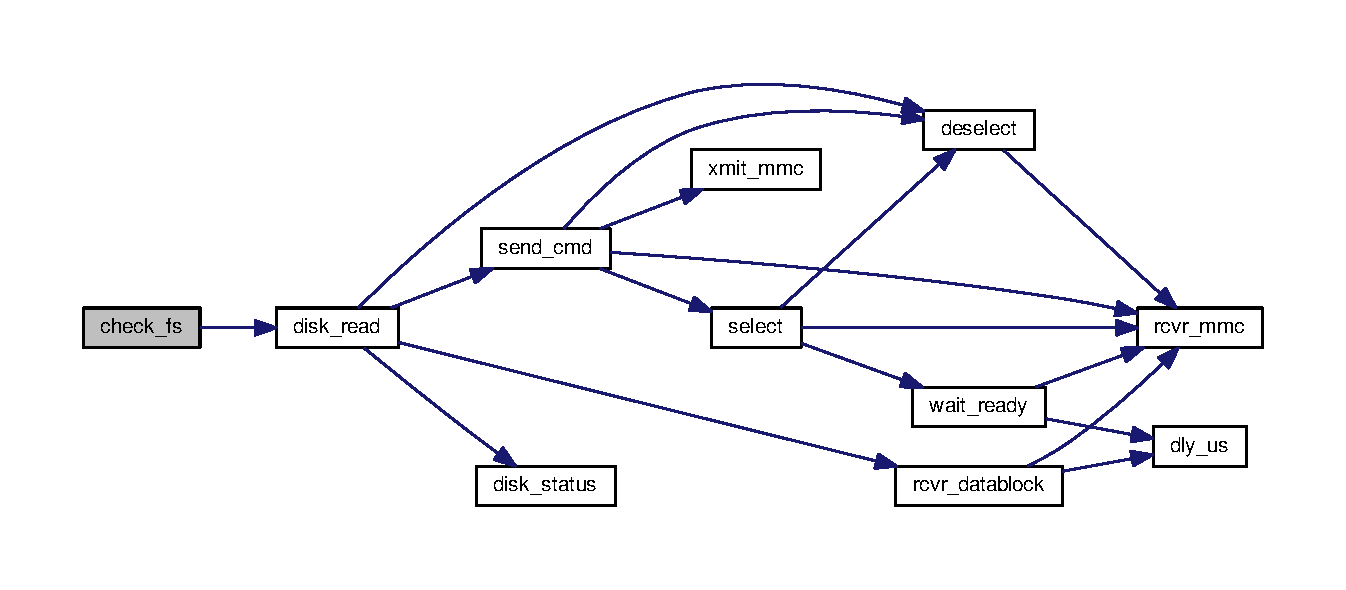
\includegraphics[width=350pt]{ff_8c_a55626c76a1556af5dc5345e2c0841a65_cgraph}
\end{center}
\end{figure}


\hypertarget{ff_8c_a1a60c4200d040e4f47e87dc927f23d14}{\index{ff.\-c@{ff.\-c}!chk\-\_\-chr@{chk\-\_\-chr}}
\index{chk\-\_\-chr@{chk\-\_\-chr}!ff.c@{ff.\-c}}
\subsubsection[{chk\-\_\-chr}]{\setlength{\rightskip}{0pt plus 5cm}static int chk\-\_\-chr (
\begin{DoxyParamCaption}
\item[{const char $\ast$}]{str, }
\item[{int}]{chr}
\end{DoxyParamCaption}
)\hspace{0.3cm}{\ttfamily [static]}}}\label{ff_8c_a1a60c4200d040e4f47e87dc927f23d14}


Referenced by create\-\_\-name(), and f\-\_\-setlabel().

\hypertarget{ff_8c_acb7ec4033afc5b9041ee9c82385552db}{\index{ff.\-c@{ff.\-c}!chk\-\_\-mounted@{chk\-\_\-mounted}}
\index{chk\-\_\-mounted@{chk\-\_\-mounted}!ff.c@{ff.\-c}}
\subsubsection[{chk\-\_\-mounted}]{\setlength{\rightskip}{0pt plus 5cm}static {\bf F\-R\-E\-S\-U\-L\-T} chk\-\_\-mounted (
\begin{DoxyParamCaption}
\item[{const {\bf T\-C\-H\-A\-R} $\ast$$\ast$}]{path, }
\item[{{\bf F\-A\-T\-F\-S} $\ast$$\ast$}]{rfs, }
\item[{{\bf B\-Y\-T\-E}}]{wmode}
\end{DoxyParamCaption}
)\hspace{0.3cm}{\ttfamily [static]}}}\label{ff_8c_acb7ec4033afc5b9041ee9c82385552db}


References \-\_\-\-F\-S\-\_\-\-R\-E\-A\-D\-O\-N\-L\-Y, \-\_\-\-V\-O\-L\-U\-M\-E\-S, B\-P\-B\-\_\-\-Byts\-Per\-Sec, B\-P\-B\-\_\-\-F\-A\-T\-Sz16, B\-P\-B\-\_\-\-F\-A\-T\-Sz32, B\-P\-B\-\_\-\-F\-S\-Info, B\-P\-B\-\_\-\-Num\-F\-A\-Ts, B\-P\-B\-\_\-\-Root\-Clus, B\-P\-B\-\_\-\-Root\-Ent\-Cnt, B\-P\-B\-\_\-\-Rsvd\-Sec\-Cnt, B\-P\-B\-\_\-\-Sec\-Per\-Clus, B\-P\-B\-\_\-\-Tot\-Sec16, B\-P\-B\-\_\-\-Tot\-Sec32, B\-S\-\_\-55\-A\-A, check\-\_\-fs(), F\-A\-T\-F\-S\-::csize, F\-A\-T\-F\-S\-::database, F\-A\-T\-F\-S\-::dirbase, disk\-\_\-initialize(), disk\-\_\-ioctl(), disk\-\_\-read(), disk\-\_\-status(), F\-A\-T\-F\-S\-::drv, E\-N\-T\-E\-R\-\_\-\-F\-F, F\-A\-T\-F\-S\-::fatbase, F\-R\-\_\-\-D\-I\-S\-K\-\_\-\-E\-R\-R, F\-R\-\_\-\-I\-N\-V\-A\-L\-I\-D\-\_\-\-D\-R\-I\-V\-E, F\-R\-\_\-\-N\-O\-\_\-\-F\-I\-L\-E\-S\-Y\-S\-T\-E\-M, F\-R\-\_\-\-N\-O\-T\-\_\-\-E\-N\-A\-B\-L\-E\-D, F\-R\-\_\-\-N\-O\-T\-\_\-\-R\-E\-A\-D\-Y, F\-R\-\_\-\-O\-K, F\-R\-\_\-\-W\-R\-I\-T\-E\-\_\-\-P\-R\-O\-T\-E\-C\-T\-E\-D, F\-A\-T\-F\-S\-::free\-\_\-clust, F\-S\-\_\-\-F\-A\-T12, F\-S\-\_\-\-F\-A\-T16, F\-S\-\_\-\-F\-A\-T32, F\-A\-T\-F\-S\-::fs\-\_\-type, F\-A\-T\-F\-S\-::fsi\-\_\-flag, F\-S\-I\-\_\-\-Free\-\_\-\-Count, F\-S\-I\-\_\-\-Lead\-Sig, F\-S\-I\-\_\-\-Nxt\-\_\-\-Free, F\-A\-T\-F\-S\-::fsi\-\_\-sector, F\-S\-I\-\_\-\-Struc\-Sig, Fsid, F\-A\-T\-F\-S\-::fsize, F\-A\-T\-F\-S\-::id, F\-A\-T\-F\-S\-::last\-\_\-clust, L\-D2\-P\-D, L\-D2\-P\-T, L\-D\-\_\-\-D\-W\-O\-R\-D, L\-D\-\_\-\-W\-O\-R\-D, M\-B\-R\-\_\-\-Table, M\-I\-N\-\_\-\-F\-A\-T16, M\-I\-N\-\_\-\-F\-A\-T32, F\-A\-T\-F\-S\-::n\-\_\-fatent, F\-A\-T\-F\-S\-::n\-\_\-fats, F\-A\-T\-F\-S\-::n\-\_\-rootdir, R\-E\-S\-\_\-\-O\-K, S\-S, S\-T\-A\-\_\-\-N\-O\-I\-N\-I\-T, S\-T\-A\-\_\-\-P\-R\-O\-T\-E\-C\-T, S\-Z\-\_\-\-D\-I\-R, S\-Z\-\_\-\-P\-T\-E, F\-A\-T\-F\-S\-::volbase, F\-A\-T\-F\-S\-::wflag, F\-A\-T\-F\-S\-::win, and F\-A\-T\-F\-S\-::winsect.



Referenced by f\-\_\-getlabel(), f\-\_\-open(), and f\-\_\-setlabel().



Here is the call graph for this function\-:
\nopagebreak
\begin{figure}[H]
\begin{center}
\leavevmode
\includegraphics[width=350pt]{ff_8c_acb7ec4033afc5b9041ee9c82385552db_cgraph}
\end{center}
\end{figure}


\hypertarget{ff_8c_a7519abb60fe91f6aa1d17f64fbae123a}{\index{ff.\-c@{ff.\-c}!clust2sect@{clust2sect}}
\index{clust2sect@{clust2sect}!ff.c@{ff.\-c}}
\subsubsection[{clust2sect}]{\setlength{\rightskip}{0pt plus 5cm}{\bf D\-W\-O\-R\-D} clust2sect (
\begin{DoxyParamCaption}
\item[{{\bf F\-A\-T\-F\-S} $\ast$}]{fs, }
\item[{{\bf D\-W\-O\-R\-D}}]{clst}
\end{DoxyParamCaption}
)}}\label{ff_8c_a7519abb60fe91f6aa1d17f64fbae123a}


References F\-A\-T\-F\-S\-::csize, F\-A\-T\-F\-S\-::database, and F\-A\-T\-F\-S\-::n\-\_\-fatent.



Referenced by dir\-\_\-next(), dir\-\_\-sdi(), f\-\_\-lseek(), f\-\_\-read(), f\-\_\-write(), and remove\-\_\-chain().

\hypertarget{ff_8c_acbd0a20a17c6f9b6d536490d1cc3c5ac}{\index{ff.\-c@{ff.\-c}!create\-\_\-chain@{create\-\_\-chain}}
\index{create\-\_\-chain@{create\-\_\-chain}!ff.c@{ff.\-c}}
\subsubsection[{create\-\_\-chain}]{\setlength{\rightskip}{0pt plus 5cm}static {\bf D\-W\-O\-R\-D} create\-\_\-chain (
\begin{DoxyParamCaption}
\item[{{\bf F\-A\-T\-F\-S} $\ast$}]{fs, }
\item[{{\bf D\-W\-O\-R\-D}}]{clst}
\end{DoxyParamCaption}
)\hspace{0.3cm}{\ttfamily [static]}}}\label{ff_8c_acbd0a20a17c6f9b6d536490d1cc3c5ac}


References F\-R\-\_\-\-D\-I\-S\-K\-\_\-\-E\-R\-R, F\-R\-\_\-\-O\-K, F\-A\-T\-F\-S\-::free\-\_\-clust, F\-A\-T\-F\-S\-::fsi\-\_\-flag, get\-\_\-fat(), F\-A\-T\-F\-S\-::last\-\_\-clust, F\-A\-T\-F\-S\-::n\-\_\-fatent, and put\-\_\-fat().



Referenced by dir\-\_\-next(), f\-\_\-lseek(), and f\-\_\-write().



Here is the call graph for this function\-:
\nopagebreak
\begin{figure}[H]
\begin{center}
\leavevmode
\includegraphics[width=350pt]{ff_8c_acbd0a20a17c6f9b6d536490d1cc3c5ac_cgraph}
\end{center}
\end{figure}


\hypertarget{ff_8c_a0bb6c133dec7b4fda00bce387e72e636}{\index{ff.\-c@{ff.\-c}!create\-\_\-name@{create\-\_\-name}}
\index{create\-\_\-name@{create\-\_\-name}!ff.c@{ff.\-c}}
\subsubsection[{create\-\_\-name}]{\setlength{\rightskip}{0pt plus 5cm}static {\bf F\-R\-E\-S\-U\-L\-T} create\-\_\-name (
\begin{DoxyParamCaption}
\item[{{\bf D\-I\-R} $\ast$}]{dj, }
\item[{const {\bf T\-C\-H\-A\-R} $\ast$$\ast$}]{path}
\end{DoxyParamCaption}
)\hspace{0.3cm}{\ttfamily [static]}}}\label{ff_8c_a0bb6c133dec7b4fda00bce387e72e636}


References \-\_\-\-D\-F1\-S, \-\_\-\-M\-A\-X\-\_\-\-L\-F\-N, chk\-\_\-chr(), D\-D\-E, Ex\-Cvt, D\-I\-R\-::fn, F\-R\-\_\-\-I\-N\-V\-A\-L\-I\-D\-\_\-\-N\-A\-M\-E, F\-R\-\_\-\-O\-K, Is\-D\-B\-C\-S1, Is\-D\-B\-C\-S2, Is\-Lower, Is\-Upper, mem\-\_\-set(), N\-D\-D\-E, N\-S, N\-S\-\_\-\-B\-O\-D\-Y, N\-S\-\_\-\-D\-O\-T, N\-S\-\_\-\-E\-X\-T, N\-S\-\_\-\-L\-A\-S\-T, N\-S\-\_\-\-L\-F\-N, and N\-S\-\_\-\-L\-O\-S\-S.



Referenced by follow\-\_\-path().



Here is the call graph for this function\-:
\nopagebreak
\begin{figure}[H]
\begin{center}
\leavevmode
\includegraphics[width=248pt]{ff_8c_a0bb6c133dec7b4fda00bce387e72e636_cgraph}
\end{center}
\end{figure}


\hypertarget{ff_8c_a42a5806b264207143a41d58a4c9ff9f1}{\index{ff.\-c@{ff.\-c}!dir\-\_\-alloc@{dir\-\_\-alloc}}
\index{dir\-\_\-alloc@{dir\-\_\-alloc}!ff.c@{ff.\-c}}
\subsubsection[{dir\-\_\-alloc}]{\setlength{\rightskip}{0pt plus 5cm}static {\bf F\-R\-E\-S\-U\-L\-T} dir\-\_\-alloc (
\begin{DoxyParamCaption}
\item[{{\bf D\-I\-R} $\ast$}]{dj, }
\item[{{\bf U\-I\-N\-T}}]{nent}
\end{DoxyParamCaption}
)\hspace{0.3cm}{\ttfamily [static]}}}\label{ff_8c_a42a5806b264207143a41d58a4c9ff9f1}


References D\-D\-E, D\-I\-R\-::dir, dir\-\_\-next(), dir\-\_\-sdi(), F\-R\-\_\-\-O\-K, D\-I\-R\-::fs, move\-\_\-window(), and D\-I\-R\-::sect.



Referenced by dir\-\_\-register(), and f\-\_\-setlabel().



Here is the call graph for this function\-:
\nopagebreak
\begin{figure}[H]
\begin{center}
\leavevmode
\includegraphics[width=350pt]{ff_8c_a42a5806b264207143a41d58a4c9ff9f1_cgraph}
\end{center}
\end{figure}


\hypertarget{ff_8c_a809fe0feb8e7a864bc048cbd22cc0702}{\index{ff.\-c@{ff.\-c}!dir\-\_\-find@{dir\-\_\-find}}
\index{dir\-\_\-find@{dir\-\_\-find}!ff.c@{ff.\-c}}
\subsubsection[{dir\-\_\-find}]{\setlength{\rightskip}{0pt plus 5cm}static {\bf F\-R\-E\-S\-U\-L\-T} dir\-\_\-find (
\begin{DoxyParamCaption}
\item[{{\bf D\-I\-R} $\ast$}]{dj}
\end{DoxyParamCaption}
)\hspace{0.3cm}{\ttfamily [static]}}}\label{ff_8c_a809fe0feb8e7a864bc048cbd22cc0702}


References A\-M\-\_\-\-L\-F\-N, A\-M\-\_\-\-M\-A\-S\-K, A\-M\-\_\-\-V\-O\-L, D\-D\-E, D\-I\-R\-::dir, D\-I\-R\-\_\-\-Attr, D\-I\-R\-\_\-\-Name, dir\-\_\-next(), dir\-\_\-sdi(), D\-I\-R\-::fn, F\-R\-\_\-\-N\-O\-\_\-\-F\-I\-L\-E, F\-R\-\_\-\-O\-K, D\-I\-R\-::fs, D\-I\-R\-::index, L\-D\-I\-R\-\_\-\-Chksum, mem\-\_\-cmp(), move\-\_\-window(), N\-S, N\-S\-\_\-\-L\-O\-S\-S, and D\-I\-R\-::sect.



Referenced by dir\-\_\-register(), and follow\-\_\-path().



Here is the call graph for this function\-:
\nopagebreak
\begin{figure}[H]
\begin{center}
\leavevmode
\includegraphics[width=350pt]{ff_8c_a809fe0feb8e7a864bc048cbd22cc0702_cgraph}
\end{center}
\end{figure}


\hypertarget{ff_8c_aa70eb326eb0c3702ae16adf0b4dce1cc}{\index{ff.\-c@{ff.\-c}!dir\-\_\-next@{dir\-\_\-next}}
\index{dir\-\_\-next@{dir\-\_\-next}!ff.c@{ff.\-c}}
\subsubsection[{dir\-\_\-next}]{\setlength{\rightskip}{0pt plus 5cm}static {\bf F\-R\-E\-S\-U\-L\-T} dir\-\_\-next (
\begin{DoxyParamCaption}
\item[{{\bf D\-I\-R} $\ast$}]{dj, }
\item[{int}]{stretch}
\end{DoxyParamCaption}
)\hspace{0.3cm}{\ttfamily [static]}}}\label{ff_8c_aa70eb326eb0c3702ae16adf0b4dce1cc}


References D\-I\-R\-::clust, clust2sect(), create\-\_\-chain(), F\-A\-T\-F\-S\-::csize, D\-I\-R\-::dir, F\-R\-\_\-\-D\-E\-N\-I\-E\-D, F\-R\-\_\-\-D\-I\-S\-K\-\_\-\-E\-R\-R, F\-R\-\_\-\-I\-N\-T\-\_\-\-E\-R\-R, F\-R\-\_\-\-N\-O\-\_\-\-F\-I\-L\-E, F\-R\-\_\-\-O\-K, D\-I\-R\-::fs, get\-\_\-fat(), D\-I\-R\-::index, mem\-\_\-set(), F\-A\-T\-F\-S\-::n\-\_\-fatent, F\-A\-T\-F\-S\-::n\-\_\-rootdir, D\-I\-R\-::sect, S\-S, sync\-\_\-window(), S\-Z\-\_\-\-D\-I\-R, F\-A\-T\-F\-S\-::wflag, F\-A\-T\-F\-S\-::win, and F\-A\-T\-F\-S\-::winsect.



Referenced by dir\-\_\-alloc(), dir\-\_\-find(), dir\-\_\-read(), and dir\-\_\-register().



Here is the call graph for this function\-:
\nopagebreak
\begin{figure}[H]
\begin{center}
\leavevmode
\includegraphics[width=350pt]{ff_8c_aa70eb326eb0c3702ae16adf0b4dce1cc_cgraph}
\end{center}
\end{figure}


\hypertarget{ff_8c_ac61cefc73baae693adfdfd86e9bd4741}{\index{ff.\-c@{ff.\-c}!dir\-\_\-read@{dir\-\_\-read}}
\index{dir\-\_\-read@{dir\-\_\-read}!ff.c@{ff.\-c}}
\subsubsection[{dir\-\_\-read}]{\setlength{\rightskip}{0pt plus 5cm}static {\bf F\-R\-E\-S\-U\-L\-T} dir\-\_\-read (
\begin{DoxyParamCaption}
\item[{{\bf D\-I\-R} $\ast$}]{dj, }
\item[{int}]{vol}
\end{DoxyParamCaption}
)\hspace{0.3cm}{\ttfamily [static]}}}\label{ff_8c_ac61cefc73baae693adfdfd86e9bd4741}


References \-\_\-\-F\-S\-\_\-\-R\-P\-A\-T\-H, A\-M\-\_\-\-L\-F\-N, A\-M\-\_\-\-M\-A\-S\-K, A\-M\-\_\-\-V\-O\-L, D\-D\-E, D\-I\-R\-::dir, D\-I\-R\-\_\-\-Attr, D\-I\-R\-\_\-\-Name, dir\-\_\-next(), F\-R\-\_\-\-N\-O\-\_\-\-F\-I\-L\-E, F\-R\-\_\-\-O\-K, D\-I\-R\-::fs, D\-I\-R\-::index, L\-D\-I\-R\-\_\-\-Chksum, move\-\_\-window(), and D\-I\-R\-::sect.



Referenced by f\-\_\-getlabel(), and f\-\_\-setlabel().



Here is the call graph for this function\-:
\nopagebreak
\begin{figure}[H]
\begin{center}
\leavevmode
\includegraphics[width=350pt]{ff_8c_ac61cefc73baae693adfdfd86e9bd4741_cgraph}
\end{center}
\end{figure}


\hypertarget{ff_8c_aa51744cb902c0cd104d3680cc05ae8b5}{\index{ff.\-c@{ff.\-c}!dir\-\_\-register@{dir\-\_\-register}}
\index{dir\-\_\-register@{dir\-\_\-register}!ff.c@{ff.\-c}}
\subsubsection[{dir\-\_\-register}]{\setlength{\rightskip}{0pt plus 5cm}static {\bf F\-R\-E\-S\-U\-L\-T} dir\-\_\-register (
\begin{DoxyParamCaption}
\item[{{\bf D\-I\-R} $\ast$}]{dj}
\end{DoxyParamCaption}
)\hspace{0.3cm}{\ttfamily [static]}}}\label{ff_8c_aa51744cb902c0cd104d3680cc05ae8b5}


References \-\_\-\-F\-S\-\_\-\-R\-P\-A\-T\-H, D\-I\-R\-::dir, dir\-\_\-alloc(), dir\-\_\-find(), dir\-\_\-next(), D\-I\-R\-\_\-\-N\-Tres, dir\-\_\-sdi(), D\-I\-R\-::fn, F\-R\-\_\-\-D\-E\-N\-I\-E\-D, F\-R\-\_\-\-I\-N\-V\-A\-L\-I\-D\-\_\-\-N\-A\-M\-E, F\-R\-\_\-\-N\-O\-\_\-\-F\-I\-L\-E, F\-R\-\_\-\-O\-K, D\-I\-R\-::fs, D\-I\-R\-::index, mem\-\_\-cpy(), mem\-\_\-set(), move\-\_\-window(), N\-S, N\-S\-\_\-\-B\-O\-D\-Y, N\-S\-\_\-\-D\-O\-T, N\-S\-\_\-\-E\-X\-T, N\-S\-\_\-\-L\-F\-N, N\-S\-\_\-\-L\-O\-S\-S, D\-I\-R\-::sect, S\-Z\-\_\-\-D\-I\-R, and F\-A\-T\-F\-S\-::wflag.



Referenced by f\-\_\-open().



Here is the call graph for this function\-:
\nopagebreak
\begin{figure}[H]
\begin{center}
\leavevmode
\includegraphics[width=350pt]{ff_8c_aa51744cb902c0cd104d3680cc05ae8b5_cgraph}
\end{center}
\end{figure}


\hypertarget{ff_8c_ad173ae134b70df2fe9668a90247567ff}{\index{ff.\-c@{ff.\-c}!dir\-\_\-sdi@{dir\-\_\-sdi}}
\index{dir\-\_\-sdi@{dir\-\_\-sdi}!ff.c@{ff.\-c}}
\subsubsection[{dir\-\_\-sdi}]{\setlength{\rightskip}{0pt plus 5cm}static {\bf F\-R\-E\-S\-U\-L\-T} dir\-\_\-sdi (
\begin{DoxyParamCaption}
\item[{{\bf D\-I\-R} $\ast$}]{dj, }
\item[{{\bf W\-O\-R\-D}}]{idx}
\end{DoxyParamCaption}
)\hspace{0.3cm}{\ttfamily [static]}}}\label{ff_8c_ad173ae134b70df2fe9668a90247567ff}


References D\-I\-R\-::clust, clust2sect(), F\-A\-T\-F\-S\-::csize, D\-I\-R\-::dir, F\-A\-T\-F\-S\-::dirbase, F\-R\-\_\-\-D\-I\-S\-K\-\_\-\-E\-R\-R, F\-R\-\_\-\-I\-N\-T\-\_\-\-E\-R\-R, F\-R\-\_\-\-O\-K, D\-I\-R\-::fs, F\-S\-\_\-\-F\-A\-T32, F\-A\-T\-F\-S\-::fs\-\_\-type, get\-\_\-fat(), D\-I\-R\-::index, F\-A\-T\-F\-S\-::n\-\_\-fatent, F\-A\-T\-F\-S\-::n\-\_\-rootdir, D\-I\-R\-::sclust, D\-I\-R\-::sect, S\-S, S\-Z\-\_\-\-D\-I\-R, and F\-A\-T\-F\-S\-::win.



Referenced by dir\-\_\-alloc(), dir\-\_\-find(), dir\-\_\-register(), f\-\_\-getlabel(), f\-\_\-setlabel(), and follow\-\_\-path().



Here is the call graph for this function\-:
\nopagebreak
\begin{figure}[H]
\begin{center}
\leavevmode
\includegraphics[width=350pt]{ff_8c_ad173ae134b70df2fe9668a90247567ff_cgraph}
\end{center}
\end{figure}


\hypertarget{ff_8c_a53882db20ef4323dcfd1874d7733ffc3}{\index{ff.\-c@{ff.\-c}!f\-\_\-close@{f\-\_\-close}}
\index{f\-\_\-close@{f\-\_\-close}!ff.c@{ff.\-c}}
\subsubsection[{f\-\_\-close}]{\setlength{\rightskip}{0pt plus 5cm}{\bf F\-R\-E\-S\-U\-L\-T} f\-\_\-close (
\begin{DoxyParamCaption}
\item[{{\bf F\-I\-L} $\ast$}]{fp}
\end{DoxyParamCaption}
)}}\label{ff_8c_a53882db20ef4323dcfd1874d7733ffc3}


References f\-\_\-sync(), F\-R\-\_\-\-O\-K, F\-I\-L\-::fs, L\-E\-A\-V\-E\-\_\-\-F\-F, and validate().



Referenced by main().



Here is the call graph for this function\-:
\nopagebreak
\begin{figure}[H]
\begin{center}
\leavevmode
\includegraphics[width=350pt]{ff_8c_a53882db20ef4323dcfd1874d7733ffc3_cgraph}
\end{center}
\end{figure}


\hypertarget{ff_8c_a430bb7b15afe7198d15a03c34641578c}{\index{ff.\-c@{ff.\-c}!f\-\_\-getlabel@{f\-\_\-getlabel}}
\index{f\-\_\-getlabel@{f\-\_\-getlabel}!ff.c@{ff.\-c}}
\subsubsection[{f\-\_\-getlabel}]{\setlength{\rightskip}{0pt plus 5cm}{\bf F\-R\-E\-S\-U\-L\-T} f\-\_\-getlabel (
\begin{DoxyParamCaption}
\item[{const {\bf T\-C\-H\-A\-R} $\ast$}]{path, }
\item[{{\bf T\-C\-H\-A\-R} $\ast$}]{label, }
\item[{{\bf D\-W\-O\-R\-D} $\ast$}]{sn}
\end{DoxyParamCaption}
)}}\label{ff_8c_a430bb7b15afe7198d15a03c34641578c}


References B\-S\-\_\-\-Vol\-I\-D, B\-S\-\_\-\-Vol\-I\-D32, chk\-\_\-mounted(), D\-I\-R\-::dir, dir\-\_\-read(), dir\-\_\-sdi(), F\-R\-\_\-\-N\-O\-\_\-\-F\-I\-L\-E, F\-R\-\_\-\-O\-K, D\-I\-R\-::fs, F\-S\-\_\-\-F\-A\-T32, F\-A\-T\-F\-S\-::fs\-\_\-type, Is\-D\-B\-C\-S1, Is\-D\-B\-C\-S2, L\-D\-\_\-\-D\-W\-O\-R\-D, L\-E\-A\-V\-E\-\_\-\-F\-F, mem\-\_\-cpy(), move\-\_\-window(), D\-I\-R\-::sclust, F\-A\-T\-F\-S\-::volbase, and F\-A\-T\-F\-S\-::win.



Referenced by main().



Here is the call graph for this function\-:
\nopagebreak
\begin{figure}[H]
\begin{center}
\leavevmode
\includegraphics[width=350pt]{ff_8c_a430bb7b15afe7198d15a03c34641578c_cgraph}
\end{center}
\end{figure}


\hypertarget{ff_8c_a5df0ac672ada972e89ef4b003e57f964}{\index{ff.\-c@{ff.\-c}!f\-\_\-lseek@{f\-\_\-lseek}}
\index{f\-\_\-lseek@{f\-\_\-lseek}!ff.c@{ff.\-c}}
\subsubsection[{f\-\_\-lseek}]{\setlength{\rightskip}{0pt plus 5cm}{\bf F\-R\-E\-S\-U\-L\-T} f\-\_\-lseek (
\begin{DoxyParamCaption}
\item[{{\bf F\-I\-L} $\ast$}]{fp, }
\item[{{\bf D\-W\-O\-R\-D}}]{ofs}
\end{DoxyParamCaption}
)}}\label{ff_8c_a5df0ac672ada972e89ef4b003e57f964}


References \-\_\-\-F\-S\-\_\-\-R\-E\-A\-D\-O\-N\-L\-Y, A\-B\-O\-R\-T, F\-I\-L\-::clust, clust2sect(), create\-\_\-chain(), C\-R\-E\-A\-T\-E\-\_\-\-L\-I\-N\-K\-M\-A\-P, F\-A\-T\-F\-S\-::csize, disk\-\_\-read(), disk\-\_\-write(), F\-A\-T\-F\-S\-::drv, F\-I\-L\-::dsect, F\-A\-\_\-\-\_\-\-D\-I\-R\-T\-Y, F\-A\-\_\-\-\_\-\-E\-R\-R\-O\-R, F\-A\-\_\-\-\_\-\-W\-R\-I\-T\-T\-E\-N, F\-A\-\_\-\-W\-R\-I\-T\-E, F\-I\-L\-::flag, F\-I\-L\-::fptr, F\-R\-\_\-\-D\-I\-S\-K\-\_\-\-E\-R\-R, F\-R\-\_\-\-I\-N\-T\-\_\-\-E\-R\-R, F\-R\-\_\-\-N\-O\-T\-\_\-\-E\-N\-O\-U\-G\-H\-\_\-\-C\-O\-R\-E, F\-R\-\_\-\-O\-K, F\-I\-L\-::fs, F\-I\-L\-::fsize, get\-\_\-fat(), L\-E\-A\-V\-E\-\_\-\-F\-F, F\-A\-T\-F\-S\-::n\-\_\-fatent, R\-E\-S\-\_\-\-O\-K, F\-I\-L\-::sclust, S\-S, and validate().



Here is the call graph for this function\-:
\nopagebreak
\begin{figure}[H]
\begin{center}
\leavevmode
\includegraphics[width=350pt]{ff_8c_a5df0ac672ada972e89ef4b003e57f964_cgraph}
\end{center}
\end{figure}


\hypertarget{ff_8c_a5f9e6982ad48becf73dc39c797e8569d}{\index{ff.\-c@{ff.\-c}!f\-\_\-mount@{f\-\_\-mount}}
\index{f\-\_\-mount@{f\-\_\-mount}!ff.c@{ff.\-c}}
\subsubsection[{f\-\_\-mount}]{\setlength{\rightskip}{0pt plus 5cm}{\bf F\-R\-E\-S\-U\-L\-T} f\-\_\-mount (
\begin{DoxyParamCaption}
\item[{{\bf B\-Y\-T\-E}}]{vol, }
\item[{{\bf F\-A\-T\-F\-S} $\ast$}]{fs}
\end{DoxyParamCaption}
)}}\label{ff_8c_a5f9e6982ad48becf73dc39c797e8569d}


References \-\_\-\-V\-O\-L\-U\-M\-E\-S, F\-R\-\_\-\-I\-N\-T\-\_\-\-E\-R\-R, F\-R\-\_\-\-I\-N\-V\-A\-L\-I\-D\-\_\-\-D\-R\-I\-V\-E, F\-R\-\_\-\-O\-K, and F\-A\-T\-F\-S\-::fs\-\_\-type.



Referenced by main().

\hypertarget{ff_8c_aefdef7126128d99d0b3bd82c28e54d80}{\index{ff.\-c@{ff.\-c}!f\-\_\-open@{f\-\_\-open}}
\index{f\-\_\-open@{f\-\_\-open}!ff.c@{ff.\-c}}
\subsubsection[{f\-\_\-open}]{\setlength{\rightskip}{0pt plus 5cm}{\bf F\-R\-E\-S\-U\-L\-T} f\-\_\-open (
\begin{DoxyParamCaption}
\item[{{\bf F\-I\-L} $\ast$}]{fp, }
\item[{const {\bf T\-C\-H\-A\-R} $\ast$}]{path, }
\item[{{\bf B\-Y\-T\-E}}]{mode}
\end{DoxyParamCaption}
)}}\label{ff_8c_aefdef7126128d99d0b3bd82c28e54d80}


References A\-M\-\_\-\-D\-I\-R, A\-M\-\_\-\-R\-D\-O, chk\-\_\-mounted(), D\-E\-F\-\_\-\-N\-A\-M\-E\-B\-U\-F, D\-I\-R\-::dir, D\-I\-R\-\_\-\-Attr, D\-I\-R\-\_\-\-Crt\-Time, D\-I\-R\-\_\-\-File\-Size, F\-I\-L\-::dir\-\_\-ptr, dir\-\_\-register(), F\-I\-L\-::dir\-\_\-sect, F\-I\-L\-::dsect, F\-A\-\_\-\-\_\-\-W\-R\-I\-T\-T\-E\-N, F\-A\-\_\-\-C\-R\-E\-A\-T\-E\-\_\-\-A\-L\-W\-A\-Y\-S, F\-A\-\_\-\-C\-R\-E\-A\-T\-E\-\_\-\-N\-E\-W, F\-A\-\_\-\-O\-P\-E\-N\-\_\-\-A\-L\-W\-A\-Y\-S, F\-A\-\_\-\-R\-E\-A\-D, F\-A\-\_\-\-W\-R\-I\-T\-E, F\-I\-L\-::flag, follow\-\_\-path(), F\-I\-L\-::fptr, F\-R\-\_\-\-D\-E\-N\-I\-E\-D, F\-R\-\_\-\-E\-X\-I\-S\-T, F\-R\-\_\-\-I\-N\-T\-\_\-\-E\-R\-R, F\-R\-\_\-\-I\-N\-V\-A\-L\-I\-D\-\_\-\-N\-A\-M\-E, F\-R\-\_\-\-I\-N\-V\-A\-L\-I\-D\-\_\-\-O\-B\-J\-E\-C\-T, F\-R\-\_\-\-N\-O\-\_\-\-F\-I\-L\-E, F\-R\-\_\-\-O\-K, F\-R\-\_\-\-T\-O\-O\-\_\-\-M\-A\-N\-Y\-\_\-\-O\-P\-E\-N\-\_\-\-F\-I\-L\-E\-S, F\-R\-E\-E\-\_\-\-B\-U\-F, F\-I\-L\-::fs, D\-I\-R\-::fs, F\-I\-L\-::fsize, get\-\_\-fattime(), F\-A\-T\-F\-S\-::id, F\-I\-L\-::id, I\-N\-I\-T\-\_\-\-B\-U\-F, F\-A\-T\-F\-S\-::last\-\_\-clust, ld\-\_\-clust(), L\-D\-\_\-\-D\-W\-O\-R\-D, L\-E\-A\-V\-E\-\_\-\-F\-F, move\-\_\-window(), remove\-\_\-chain(), F\-I\-L\-::sclust, st\-\_\-clust(), S\-T\-\_\-\-D\-W\-O\-R\-D, F\-A\-T\-F\-S\-::wflag, and F\-A\-T\-F\-S\-::winsect.



Referenced by main().



Here is the call graph for this function\-:
\nopagebreak
\begin{figure}[H]
\begin{center}
\leavevmode
\includegraphics[width=350pt]{ff_8c_aefdef7126128d99d0b3bd82c28e54d80_cgraph}
\end{center}
\end{figure}


\hypertarget{ff_8c_ac4c3dcb6869ca252888eebabe39727b3}{\index{ff.\-c@{ff.\-c}!f\-\_\-read@{f\-\_\-read}}
\index{f\-\_\-read@{f\-\_\-read}!ff.c@{ff.\-c}}
\subsubsection[{f\-\_\-read}]{\setlength{\rightskip}{0pt plus 5cm}{\bf F\-R\-E\-S\-U\-L\-T} f\-\_\-read (
\begin{DoxyParamCaption}
\item[{{\bf F\-I\-L} $\ast$}]{fp, }
\item[{void $\ast$}]{buff, }
\item[{{\bf U\-I\-N\-T}}]{btr, }
\item[{{\bf U\-I\-N\-T} $\ast$}]{br}
\end{DoxyParamCaption}
)}}\label{ff_8c_ac4c3dcb6869ca252888eebabe39727b3}


References A\-B\-O\-R\-T, F\-I\-L\-::clust, clust2sect(), F\-A\-T\-F\-S\-::csize, disk\-\_\-read(), disk\-\_\-write(), F\-A\-T\-F\-S\-::drv, F\-I\-L\-::dsect, F\-A\-\_\-\-\_\-\-D\-I\-R\-T\-Y, F\-A\-\_\-\-\_\-\-E\-R\-R\-O\-R, F\-A\-\_\-\-R\-E\-A\-D, F\-I\-L\-::flag, F\-I\-L\-::fptr, F\-R\-\_\-\-D\-E\-N\-I\-E\-D, F\-R\-\_\-\-D\-I\-S\-K\-\_\-\-E\-R\-R, F\-R\-\_\-\-I\-N\-T\-\_\-\-E\-R\-R, F\-R\-\_\-\-O\-K, F\-I\-L\-::fs, F\-I\-L\-::fsize, get\-\_\-fat(), L\-E\-A\-V\-E\-\_\-\-F\-F, mem\-\_\-cpy(), move\-\_\-window(), R\-E\-S\-\_\-\-O\-K, F\-I\-L\-::sclust, S\-S, validate(), F\-A\-T\-F\-S\-::wflag, F\-A\-T\-F\-S\-::win, and F\-A\-T\-F\-S\-::winsect.



Referenced by main().



Here is the call graph for this function\-:
\nopagebreak
\begin{figure}[H]
\begin{center}
\leavevmode
\includegraphics[width=350pt]{ff_8c_ac4c3dcb6869ca252888eebabe39727b3_cgraph}
\end{center}
\end{figure}


\hypertarget{ff_8c_aa82bca64e28bc0d656a7999dd0eadec7}{\index{ff.\-c@{ff.\-c}!f\-\_\-setlabel@{f\-\_\-setlabel}}
\index{f\-\_\-setlabel@{f\-\_\-setlabel}!ff.c@{ff.\-c}}
\subsubsection[{f\-\_\-setlabel}]{\setlength{\rightskip}{0pt plus 5cm}{\bf F\-R\-E\-S\-U\-L\-T} f\-\_\-setlabel (
\begin{DoxyParamCaption}
\item[{const {\bf T\-C\-H\-A\-R} $\ast$}]{label}
\end{DoxyParamCaption}
)}}\label{ff_8c_aa82bca64e28bc0d656a7999dd0eadec7}


References \-\_\-\-D\-F1\-S, A\-M\-\_\-\-V\-O\-L, chk\-\_\-chr(), chk\-\_\-mounted(), D\-D\-E, D\-I\-R\-::dir, dir\-\_\-alloc(), D\-I\-R\-\_\-\-Attr, dir\-\_\-read(), dir\-\_\-sdi(), D\-I\-R\-\_\-\-Wrt\-Time, Ex\-Cvt, F\-R\-\_\-\-I\-N\-V\-A\-L\-I\-D\-\_\-\-N\-A\-M\-E, F\-R\-\_\-\-N\-O\-\_\-\-F\-I\-L\-E, F\-R\-\_\-\-O\-K, D\-I\-R\-::fs, get\-\_\-fattime(), Is\-D\-B\-C\-S1, Is\-D\-B\-C\-S2, Is\-Lower, L\-E\-A\-V\-E\-\_\-\-F\-F, mem\-\_\-cpy(), mem\-\_\-set(), D\-I\-R\-::sclust, S\-T\-\_\-\-D\-W\-O\-R\-D, sync\-\_\-fs(), S\-Z\-\_\-\-D\-I\-R, and F\-A\-T\-F\-S\-::wflag.



Here is the call graph for this function\-:
\nopagebreak
\begin{figure}[H]
\begin{center}
\leavevmode
\includegraphics[width=350pt]{ff_8c_aa82bca64e28bc0d656a7999dd0eadec7_cgraph}
\end{center}
\end{figure}


\hypertarget{ff_8c_ad69c7246b122ba56a134939ee0eaf847}{\index{ff.\-c@{ff.\-c}!f\-\_\-sync@{f\-\_\-sync}}
\index{f\-\_\-sync@{f\-\_\-sync}!ff.c@{ff.\-c}}
\subsubsection[{f\-\_\-sync}]{\setlength{\rightskip}{0pt plus 5cm}{\bf F\-R\-E\-S\-U\-L\-T} f\-\_\-sync (
\begin{DoxyParamCaption}
\item[{{\bf F\-I\-L} $\ast$}]{fp}
\end{DoxyParamCaption}
)}}\label{ff_8c_ad69c7246b122ba56a134939ee0eaf847}


References A\-M\-\_\-\-A\-R\-C, D\-I\-R\-\_\-\-Attr, D\-I\-R\-\_\-\-File\-Size, D\-I\-R\-\_\-\-Lst\-Acc\-Date, F\-I\-L\-::dir\-\_\-ptr, F\-I\-L\-::dir\-\_\-sect, D\-I\-R\-\_\-\-Wrt\-Time, disk\-\_\-write(), F\-A\-T\-F\-S\-::drv, F\-I\-L\-::dsect, F\-A\-\_\-\-\_\-\-D\-I\-R\-T\-Y, F\-A\-\_\-\-\_\-\-W\-R\-I\-T\-T\-E\-N, F\-I\-L\-::flag, F\-R\-\_\-\-D\-I\-S\-K\-\_\-\-E\-R\-R, F\-R\-\_\-\-O\-K, F\-I\-L\-::fs, F\-I\-L\-::fsize, get\-\_\-fattime(), L\-E\-A\-V\-E\-\_\-\-F\-F, move\-\_\-window(), R\-E\-S\-\_\-\-O\-K, F\-I\-L\-::sclust, st\-\_\-clust(), S\-T\-\_\-\-D\-W\-O\-R\-D, S\-T\-\_\-\-W\-O\-R\-D, sync\-\_\-fs(), validate(), and F\-A\-T\-F\-S\-::wflag.



Referenced by f\-\_\-close().



Here is the call graph for this function\-:
\nopagebreak
\begin{figure}[H]
\begin{center}
\leavevmode
\includegraphics[width=350pt]{ff_8c_ad69c7246b122ba56a134939ee0eaf847_cgraph}
\end{center}
\end{figure}


\hypertarget{ff_8c_ae6a4dfae8a9e308bdb2283a37ef680f2}{\index{ff.\-c@{ff.\-c}!f\-\_\-write@{f\-\_\-write}}
\index{f\-\_\-write@{f\-\_\-write}!ff.c@{ff.\-c}}
\subsubsection[{f\-\_\-write}]{\setlength{\rightskip}{0pt plus 5cm}{\bf F\-R\-E\-S\-U\-L\-T} f\-\_\-write (
\begin{DoxyParamCaption}
\item[{{\bf F\-I\-L} $\ast$}]{fp, }
\item[{const void $\ast$}]{buff, }
\item[{{\bf U\-I\-N\-T}}]{btw, }
\item[{{\bf U\-I\-N\-T} $\ast$}]{bw}
\end{DoxyParamCaption}
)}}\label{ff_8c_ae6a4dfae8a9e308bdb2283a37ef680f2}


References A\-B\-O\-R\-T, F\-I\-L\-::clust, clust2sect(), create\-\_\-chain(), F\-A\-T\-F\-S\-::csize, disk\-\_\-read(), disk\-\_\-write(), F\-A\-T\-F\-S\-::drv, F\-I\-L\-::dsect, F\-A\-\_\-\-\_\-\-D\-I\-R\-T\-Y, F\-A\-\_\-\-\_\-\-E\-R\-R\-O\-R, F\-A\-\_\-\-\_\-\-W\-R\-I\-T\-T\-E\-N, F\-A\-\_\-\-W\-R\-I\-T\-E, F\-I\-L\-::flag, F\-I\-L\-::fptr, F\-R\-\_\-\-D\-E\-N\-I\-E\-D, F\-R\-\_\-\-D\-I\-S\-K\-\_\-\-E\-R\-R, F\-R\-\_\-\-I\-N\-T\-\_\-\-E\-R\-R, F\-R\-\_\-\-O\-K, F\-I\-L\-::fs, F\-I\-L\-::fsize, L\-E\-A\-V\-E\-\_\-\-F\-F, mem\-\_\-cpy(), move\-\_\-window(), R\-E\-S\-\_\-\-O\-K, F\-I\-L\-::sclust, S\-S, sync\-\_\-window(), validate(), F\-A\-T\-F\-S\-::wflag, F\-A\-T\-F\-S\-::win, and F\-A\-T\-F\-S\-::winsect.



Referenced by main().



Here is the call graph for this function\-:
\nopagebreak
\begin{figure}[H]
\begin{center}
\leavevmode
\includegraphics[width=350pt]{ff_8c_ae6a4dfae8a9e308bdb2283a37ef680f2_cgraph}
\end{center}
\end{figure}


\hypertarget{ff_8c_aac9a82c50bb738b3d78d4a46ffdad65d}{\index{ff.\-c@{ff.\-c}!follow\-\_\-path@{follow\-\_\-path}}
\index{follow\-\_\-path@{follow\-\_\-path}!ff.c@{ff.\-c}}
\subsubsection[{follow\-\_\-path}]{\setlength{\rightskip}{0pt plus 5cm}static {\bf F\-R\-E\-S\-U\-L\-T} follow\-\_\-path (
\begin{DoxyParamCaption}
\item[{{\bf D\-I\-R} $\ast$}]{dj, }
\item[{const {\bf T\-C\-H\-A\-R} $\ast$}]{path}
\end{DoxyParamCaption}
)\hspace{0.3cm}{\ttfamily [static]}}}\label{ff_8c_aac9a82c50bb738b3d78d4a46ffdad65d}


References \-\_\-\-F\-S\-\_\-\-R\-P\-A\-T\-H, A\-M\-\_\-\-D\-I\-R, create\-\_\-name(), D\-I\-R\-::dir, D\-I\-R\-\_\-\-Attr, dir\-\_\-find(), dir\-\_\-sdi(), D\-I\-R\-::fn, F\-R\-\_\-\-N\-O\-\_\-\-F\-I\-L\-E, F\-R\-\_\-\-N\-O\-\_\-\-P\-A\-T\-H, F\-R\-\_\-\-O\-K, D\-I\-R\-::fs, ld\-\_\-clust(), N\-S, N\-S\-\_\-\-D\-O\-T, N\-S\-\_\-\-L\-A\-S\-T, and D\-I\-R\-::sclust.



Referenced by f\-\_\-open().



Here is the call graph for this function\-:
\nopagebreak
\begin{figure}[H]
\begin{center}
\leavevmode
\includegraphics[width=350pt]{ff_8c_aac9a82c50bb738b3d78d4a46ffdad65d_cgraph}
\end{center}
\end{figure}


\hypertarget{ff_8c_a65611adf1626e5e08da77cd33a98dd8b}{\index{ff.\-c@{ff.\-c}!get\-\_\-fat@{get\-\_\-fat}}
\index{get\-\_\-fat@{get\-\_\-fat}!ff.c@{ff.\-c}}
\subsubsection[{get\-\_\-fat}]{\setlength{\rightskip}{0pt plus 5cm}{\bf D\-W\-O\-R\-D} get\-\_\-fat (
\begin{DoxyParamCaption}
\item[{{\bf F\-A\-T\-F\-S} $\ast$}]{fs, }
\item[{{\bf D\-W\-O\-R\-D}}]{clst}
\end{DoxyParamCaption}
)}}\label{ff_8c_a65611adf1626e5e08da77cd33a98dd8b}


References F\-A\-T\-F\-S\-::fatbase, F\-S\-\_\-\-F\-A\-T12, F\-S\-\_\-\-F\-A\-T16, F\-S\-\_\-\-F\-A\-T32, F\-A\-T\-F\-S\-::fs\-\_\-type, L\-D\-\_\-\-D\-W\-O\-R\-D, L\-D\-\_\-\-W\-O\-R\-D, move\-\_\-window(), F\-A\-T\-F\-S\-::n\-\_\-fatent, S\-S, and F\-A\-T\-F\-S\-::win.



Referenced by create\-\_\-chain(), dir\-\_\-next(), dir\-\_\-sdi(), f\-\_\-lseek(), f\-\_\-read(), and remove\-\_\-chain().



Here is the call graph for this function\-:
\nopagebreak
\begin{figure}[H]
\begin{center}
\leavevmode
\includegraphics[width=350pt]{ff_8c_a65611adf1626e5e08da77cd33a98dd8b_cgraph}
\end{center}
\end{figure}


\hypertarget{ff_8c_a996d46ee1f9aed650880aecb4b7eb314}{\index{ff.\-c@{ff.\-c}!ld\-\_\-clust@{ld\-\_\-clust}}
\index{ld\-\_\-clust@{ld\-\_\-clust}!ff.c@{ff.\-c}}
\subsubsection[{ld\-\_\-clust}]{\setlength{\rightskip}{0pt plus 5cm}static {\bf D\-W\-O\-R\-D} ld\-\_\-clust (
\begin{DoxyParamCaption}
\item[{{\bf F\-A\-T\-F\-S} $\ast$}]{fs, }
\item[{{\bf B\-Y\-T\-E} $\ast$}]{dir}
\end{DoxyParamCaption}
)\hspace{0.3cm}{\ttfamily [static]}}}\label{ff_8c_a996d46ee1f9aed650880aecb4b7eb314}


References D\-I\-R\-\_\-\-Fst\-Clus\-H\-I, D\-I\-R\-\_\-\-Fst\-Clus\-L\-O, F\-S\-\_\-\-F\-A\-T32, F\-A\-T\-F\-S\-::fs\-\_\-type, and L\-D\-\_\-\-W\-O\-R\-D.



Referenced by f\-\_\-open(), and follow\-\_\-path().

\hypertarget{ff_8c_a38b4f223d18bd4416d8bce0f07a63c01}{\index{ff.\-c@{ff.\-c}!mem\-\_\-cmp@{mem\-\_\-cmp}}
\index{mem\-\_\-cmp@{mem\-\_\-cmp}!ff.c@{ff.\-c}}
\subsubsection[{mem\-\_\-cmp}]{\setlength{\rightskip}{0pt plus 5cm}static int mem\-\_\-cmp (
\begin{DoxyParamCaption}
\item[{const void $\ast$}]{dst, }
\item[{const void $\ast$}]{src, }
\item[{{\bf U\-I\-N\-T}}]{cnt}
\end{DoxyParamCaption}
)\hspace{0.3cm}{\ttfamily [static]}}}\label{ff_8c_a38b4f223d18bd4416d8bce0f07a63c01}


Referenced by dir\-\_\-find().

\hypertarget{ff_8c_a8941d573d16af92c8570950d53164f30}{\index{ff.\-c@{ff.\-c}!mem\-\_\-cpy@{mem\-\_\-cpy}}
\index{mem\-\_\-cpy@{mem\-\_\-cpy}!ff.c@{ff.\-c}}
\subsubsection[{mem\-\_\-cpy}]{\setlength{\rightskip}{0pt plus 5cm}static void mem\-\_\-cpy (
\begin{DoxyParamCaption}
\item[{void $\ast$}]{dst, }
\item[{const void $\ast$}]{src, }
\item[{{\bf U\-I\-N\-T}}]{cnt}
\end{DoxyParamCaption}
)\hspace{0.3cm}{\ttfamily [static]}}}\label{ff_8c_a8941d573d16af92c8570950d53164f30}


Referenced by dir\-\_\-register(), f\-\_\-getlabel(), f\-\_\-read(), f\-\_\-setlabel(), and f\-\_\-write().

\hypertarget{ff_8c_a02eb5189e43056a9ddc8a59cbe89be93}{\index{ff.\-c@{ff.\-c}!mem\-\_\-set@{mem\-\_\-set}}
\index{mem\-\_\-set@{mem\-\_\-set}!ff.c@{ff.\-c}}
\subsubsection[{mem\-\_\-set}]{\setlength{\rightskip}{0pt plus 5cm}static void mem\-\_\-set (
\begin{DoxyParamCaption}
\item[{void $\ast$}]{dst, }
\item[{int}]{val, }
\item[{{\bf U\-I\-N\-T}}]{cnt}
\end{DoxyParamCaption}
)\hspace{0.3cm}{\ttfamily [static]}}}\label{ff_8c_a02eb5189e43056a9ddc8a59cbe89be93}


Referenced by create\-\_\-name(), dir\-\_\-next(), dir\-\_\-register(), f\-\_\-setlabel(), and sync\-\_\-fs().

\hypertarget{ff_8c_af2e8986556ee6644b4bf31fa4158d735}{\index{ff.\-c@{ff.\-c}!move\-\_\-window@{move\-\_\-window}}
\index{move\-\_\-window@{move\-\_\-window}!ff.c@{ff.\-c}}
\subsubsection[{move\-\_\-window}]{\setlength{\rightskip}{0pt plus 5cm}static {\bf F\-R\-E\-S\-U\-L\-T} move\-\_\-window (
\begin{DoxyParamCaption}
\item[{{\bf F\-A\-T\-F\-S} $\ast$}]{fs, }
\item[{{\bf D\-W\-O\-R\-D}}]{sector}
\end{DoxyParamCaption}
)\hspace{0.3cm}{\ttfamily [static]}}}\label{ff_8c_af2e8986556ee6644b4bf31fa4158d735}


References disk\-\_\-read(), F\-A\-T\-F\-S\-::drv, F\-R\-\_\-\-D\-I\-S\-K\-\_\-\-E\-R\-R, F\-R\-\_\-\-O\-K, R\-E\-S\-\_\-\-O\-K, sync\-\_\-window(), F\-A\-T\-F\-S\-::win, and F\-A\-T\-F\-S\-::winsect.



Referenced by dir\-\_\-alloc(), dir\-\_\-find(), dir\-\_\-read(), dir\-\_\-register(), f\-\_\-getlabel(), f\-\_\-open(), f\-\_\-read(), f\-\_\-sync(), f\-\_\-write(), get\-\_\-fat(), and put\-\_\-fat().



Here is the call graph for this function\-:
\nopagebreak
\begin{figure}[H]
\begin{center}
\leavevmode
\includegraphics[width=350pt]{ff_8c_af2e8986556ee6644b4bf31fa4158d735_cgraph}
\end{center}
\end{figure}


\hypertarget{ff_8c_abd4b6b071a8d728a88727051c12bc6d7}{\index{ff.\-c@{ff.\-c}!put\-\_\-fat@{put\-\_\-fat}}
\index{put\-\_\-fat@{put\-\_\-fat}!ff.c@{ff.\-c}}
\subsubsection[{put\-\_\-fat}]{\setlength{\rightskip}{0pt plus 5cm}{\bf F\-R\-E\-S\-U\-L\-T} put\-\_\-fat (
\begin{DoxyParamCaption}
\item[{{\bf F\-A\-T\-F\-S} $\ast$}]{fs, }
\item[{{\bf D\-W\-O\-R\-D}}]{clst, }
\item[{{\bf D\-W\-O\-R\-D}}]{val}
\end{DoxyParamCaption}
)}}\label{ff_8c_abd4b6b071a8d728a88727051c12bc6d7}


References F\-A\-T\-F\-S\-::fatbase, F\-R\-\_\-\-I\-N\-T\-\_\-\-E\-R\-R, F\-R\-\_\-\-O\-K, F\-S\-\_\-\-F\-A\-T12, F\-S\-\_\-\-F\-A\-T16, F\-S\-\_\-\-F\-A\-T32, F\-A\-T\-F\-S\-::fs\-\_\-type, L\-D\-\_\-\-D\-W\-O\-R\-D, move\-\_\-window(), F\-A\-T\-F\-S\-::n\-\_\-fatent, S\-S, S\-T\-\_\-\-D\-W\-O\-R\-D, S\-T\-\_\-\-W\-O\-R\-D, F\-A\-T\-F\-S\-::wflag, and F\-A\-T\-F\-S\-::win.



Referenced by create\-\_\-chain(), and remove\-\_\-chain().



Here is the call graph for this function\-:
\nopagebreak
\begin{figure}[H]
\begin{center}
\leavevmode
\includegraphics[width=350pt]{ff_8c_abd4b6b071a8d728a88727051c12bc6d7_cgraph}
\end{center}
\end{figure}


\hypertarget{ff_8c_ab88651d19a5597dec220fe7538cccf23}{\index{ff.\-c@{ff.\-c}!remove\-\_\-chain@{remove\-\_\-chain}}
\index{remove\-\_\-chain@{remove\-\_\-chain}!ff.c@{ff.\-c}}
\subsubsection[{remove\-\_\-chain}]{\setlength{\rightskip}{0pt plus 5cm}static {\bf F\-R\-E\-S\-U\-L\-T} remove\-\_\-chain (
\begin{DoxyParamCaption}
\item[{{\bf F\-A\-T\-F\-S} $\ast$}]{fs, }
\item[{{\bf D\-W\-O\-R\-D}}]{clst}
\end{DoxyParamCaption}
)\hspace{0.3cm}{\ttfamily [static]}}}\label{ff_8c_ab88651d19a5597dec220fe7538cccf23}


References clust2sect(), F\-A\-T\-F\-S\-::csize, C\-T\-R\-L\-\_\-\-E\-R\-A\-S\-E\-\_\-\-S\-E\-C\-T\-O\-R, disk\-\_\-ioctl(), F\-A\-T\-F\-S\-::drv, F\-R\-\_\-\-D\-I\-S\-K\-\_\-\-E\-R\-R, F\-R\-\_\-\-I\-N\-T\-\_\-\-E\-R\-R, F\-R\-\_\-\-O\-K, F\-A\-T\-F\-S\-::free\-\_\-clust, F\-A\-T\-F\-S\-::fsi\-\_\-flag, get\-\_\-fat(), F\-A\-T\-F\-S\-::n\-\_\-fatent, and put\-\_\-fat().



Referenced by f\-\_\-open().



Here is the call graph for this function\-:
\nopagebreak
\begin{figure}[H]
\begin{center}
\leavevmode
\includegraphics[width=350pt]{ff_8c_ab88651d19a5597dec220fe7538cccf23_cgraph}
\end{center}
\end{figure}


\hypertarget{ff_8c_a357e5a36452e057d68378c98cd61018c}{\index{ff.\-c@{ff.\-c}!st\-\_\-clust@{st\-\_\-clust}}
\index{st\-\_\-clust@{st\-\_\-clust}!ff.c@{ff.\-c}}
\subsubsection[{st\-\_\-clust}]{\setlength{\rightskip}{0pt plus 5cm}static void st\-\_\-clust (
\begin{DoxyParamCaption}
\item[{{\bf B\-Y\-T\-E} $\ast$}]{dir, }
\item[{{\bf D\-W\-O\-R\-D}}]{cl}
\end{DoxyParamCaption}
)\hspace{0.3cm}{\ttfamily [static]}}}\label{ff_8c_a357e5a36452e057d68378c98cd61018c}


References D\-I\-R\-\_\-\-Fst\-Clus\-H\-I, D\-I\-R\-\_\-\-Fst\-Clus\-L\-O, and S\-T\-\_\-\-W\-O\-R\-D.



Referenced by f\-\_\-open(), and f\-\_\-sync().

\hypertarget{ff_8c_aec6b108298553219ebb2b960b528459d}{\index{ff.\-c@{ff.\-c}!sync\-\_\-fs@{sync\-\_\-fs}}
\index{sync\-\_\-fs@{sync\-\_\-fs}!ff.c@{ff.\-c}}
\subsubsection[{sync\-\_\-fs}]{\setlength{\rightskip}{0pt plus 5cm}static {\bf F\-R\-E\-S\-U\-L\-T} sync\-\_\-fs (
\begin{DoxyParamCaption}
\item[{{\bf F\-A\-T\-F\-S} $\ast$}]{fs}
\end{DoxyParamCaption}
)\hspace{0.3cm}{\ttfamily [static]}}}\label{ff_8c_aec6b108298553219ebb2b960b528459d}


References B\-S\-\_\-55\-A\-A, C\-T\-R\-L\-\_\-\-S\-Y\-N\-C, disk\-\_\-ioctl(), disk\-\_\-write(), F\-A\-T\-F\-S\-::drv, F\-R\-\_\-\-D\-I\-S\-K\-\_\-\-E\-R\-R, F\-R\-\_\-\-O\-K, F\-A\-T\-F\-S\-::free\-\_\-clust, F\-S\-\_\-\-F\-A\-T32, F\-A\-T\-F\-S\-::fs\-\_\-type, F\-A\-T\-F\-S\-::fsi\-\_\-flag, F\-S\-I\-\_\-\-Free\-\_\-\-Count, F\-S\-I\-\_\-\-Lead\-Sig, F\-S\-I\-\_\-\-Nxt\-\_\-\-Free, F\-A\-T\-F\-S\-::fsi\-\_\-sector, F\-S\-I\-\_\-\-Struc\-Sig, F\-A\-T\-F\-S\-::last\-\_\-clust, mem\-\_\-set(), R\-E\-S\-\_\-\-O\-K, S\-T\-\_\-\-D\-W\-O\-R\-D, S\-T\-\_\-\-W\-O\-R\-D, sync\-\_\-window(), F\-A\-T\-F\-S\-::win, and F\-A\-T\-F\-S\-::winsect.



Referenced by f\-\_\-setlabel(), and f\-\_\-sync().



Here is the call graph for this function\-:
\nopagebreak
\begin{figure}[H]
\begin{center}
\leavevmode
\includegraphics[width=350pt]{ff_8c_aec6b108298553219ebb2b960b528459d_cgraph}
\end{center}
\end{figure}


\hypertarget{ff_8c_a5e18753404354b210096f9af99e31bc1}{\index{ff.\-c@{ff.\-c}!sync\-\_\-window@{sync\-\_\-window}}
\index{sync\-\_\-window@{sync\-\_\-window}!ff.c@{ff.\-c}}
\subsubsection[{sync\-\_\-window}]{\setlength{\rightskip}{0pt plus 5cm}static {\bf F\-R\-E\-S\-U\-L\-T} sync\-\_\-window (
\begin{DoxyParamCaption}
\item[{{\bf F\-A\-T\-F\-S} $\ast$}]{fs}
\end{DoxyParamCaption}
)\hspace{0.3cm}{\ttfamily [static]}}}\label{ff_8c_a5e18753404354b210096f9af99e31bc1}


References disk\-\_\-write(), F\-A\-T\-F\-S\-::drv, F\-A\-T\-F\-S\-::fatbase, F\-R\-\_\-\-D\-I\-S\-K\-\_\-\-E\-R\-R, F\-R\-\_\-\-O\-K, F\-A\-T\-F\-S\-::fsize, F\-A\-T\-F\-S\-::n\-\_\-fats, R\-E\-S\-\_\-\-O\-K, F\-A\-T\-F\-S\-::wflag, F\-A\-T\-F\-S\-::win, and F\-A\-T\-F\-S\-::winsect.



Referenced by dir\-\_\-next(), f\-\_\-write(), move\-\_\-window(), and sync\-\_\-fs().



Here is the call graph for this function\-:
\nopagebreak
\begin{figure}[H]
\begin{center}
\leavevmode
\includegraphics[width=350pt]{ff_8c_a5e18753404354b210096f9af99e31bc1_cgraph}
\end{center}
\end{figure}


\hypertarget{ff_8c_aa7193f5b86c3996b5312043a0c26da5f}{\index{ff.\-c@{ff.\-c}!validate@{validate}}
\index{validate@{validate}!ff.c@{ff.\-c}}
\subsubsection[{validate}]{\setlength{\rightskip}{0pt plus 5cm}static {\bf F\-R\-E\-S\-U\-L\-T} validate (
\begin{DoxyParamCaption}
\item[{void $\ast$}]{obj}
\end{DoxyParamCaption}
)\hspace{0.3cm}{\ttfamily [static]}}}\label{ff_8c_aa7193f5b86c3996b5312043a0c26da5f}


References disk\-\_\-status(), F\-A\-T\-F\-S\-::drv, E\-N\-T\-E\-R\-\_\-\-F\-F, F\-R\-\_\-\-I\-N\-V\-A\-L\-I\-D\-\_\-\-O\-B\-J\-E\-C\-T, F\-R\-\_\-\-N\-O\-T\-\_\-\-R\-E\-A\-D\-Y, F\-R\-\_\-\-O\-K, F\-I\-L\-::fs, F\-A\-T\-F\-S\-::fs\-\_\-type, F\-A\-T\-F\-S\-::id, F\-I\-L\-::id, and S\-T\-A\-\_\-\-N\-O\-I\-N\-I\-T.



Referenced by f\-\_\-close(), f\-\_\-lseek(), f\-\_\-read(), f\-\_\-sync(), and f\-\_\-write().



Here is the call graph for this function\-:
\nopagebreak
\begin{figure}[H]
\begin{center}
\leavevmode
\includegraphics[width=234pt]{ff_8c_aa7193f5b86c3996b5312043a0c26da5f_cgraph}
\end{center}
\end{figure}




\subsection{Variable Documentation}
\hypertarget{ff_8c_aded249c8b2fc2c9ca7997e028d07771b}{\index{ff.\-c@{ff.\-c}!Ex\-Cvt@{Ex\-Cvt}}
\index{Ex\-Cvt@{Ex\-Cvt}!ff.c@{ff.\-c}}
\subsubsection[{Ex\-Cvt}]{\setlength{\rightskip}{0pt plus 5cm}const {\bf B\-Y\-T\-E} Ex\-Cvt\mbox{[}$\,$\mbox{]} = {\bf \-\_\-\-E\-X\-C\-V\-T}\hspace{0.3cm}{\ttfamily [static]}}}\label{ff_8c_aded249c8b2fc2c9ca7997e028d07771b}


Referenced by create\-\_\-name(), and f\-\_\-setlabel().

\hypertarget{ff_8c_a3d7aad0939745576943767bf6c410eaf}{\index{ff.\-c@{ff.\-c}!Fat\-Fs@{Fat\-Fs}}
\index{Fat\-Fs@{Fat\-Fs}!ff.c@{ff.\-c}}
\subsubsection[{Fat\-Fs}]{\setlength{\rightskip}{0pt plus 5cm}{\bf F\-A\-T\-F\-S}$\ast$ Fat\-Fs\mbox{[}{\bf \-\_\-\-V\-O\-L\-U\-M\-E\-S}\mbox{]}\hspace{0.3cm}{\ttfamily [static]}}}\label{ff_8c_a3d7aad0939745576943767bf6c410eaf}
\hypertarget{ff_8c_a0b3f41d8c416222e9b1c16e36d66e18b}{\index{ff.\-c@{ff.\-c}!Fsid@{Fsid}}
\index{Fsid@{Fsid}!ff.c@{ff.\-c}}
\subsubsection[{Fsid}]{\setlength{\rightskip}{0pt plus 5cm}{\bf W\-O\-R\-D} Fsid\hspace{0.3cm}{\ttfamily [static]}}}\label{ff_8c_a0b3f41d8c416222e9b1c16e36d66e18b}


Referenced by chk\-\_\-mounted().


\hypertarget{ff_8h}{\section{sd\-\_\-card/ff.h File Reference}
\label{ff_8h}\index{sd\-\_\-card/ff.\-h@{sd\-\_\-card/ff.\-h}}
}
{\ttfamily \#include \char`\"{}integer.\-h\char`\"{}}\\*
{\ttfamily \#include \char`\"{}ffconf.\-h\char`\"{}}\\*
Include dependency graph for ff.\-h\-:\nopagebreak
\begin{figure}[H]
\begin{center}
\leavevmode
\includegraphics[width=202pt]{ff_8h__incl}
\end{center}
\end{figure}
This graph shows which files directly or indirectly include this file\-:\nopagebreak
\begin{figure}[H]
\begin{center}
\leavevmode
\includegraphics[width=212pt]{ff_8h__dep__incl}
\end{center}
\end{figure}
\subsection*{Data Structures}
\begin{DoxyCompactItemize}
\item 
struct \hyperlink{structFATFS}{F\-A\-T\-F\-S}
\item 
struct \hyperlink{structFIL}{F\-I\-L}
\item 
struct \hyperlink{structDIR}{D\-I\-R}
\item 
struct \hyperlink{structFILINFO}{F\-I\-L\-I\-N\-F\-O}
\end{DoxyCompactItemize}
\subsection*{Macros}
\begin{DoxyCompactItemize}
\item 
\#define \hyperlink{ff_8h_a749228947bc890224b8bd5de6e11faa3}{\-\_\-\-F\-A\-T\-F\-S}~82786	/$\ast$ Revision I\-D $\ast$/
\item 
\#define \hyperlink{ff_8h_a6577ed2f95527745bf4d27c53488b9a7}{L\-D2\-P\-D}(vol)~(\hyperlink{integer_8h_a4ae1dab0fb4b072a66584546209e7d58}{B\-Y\-T\-E})(vol)	/$\ast$ Each logical drive is bound to the same physical drive number $\ast$/
\item 
\#define \hyperlink{ff_8h_aadc4a9aefaf2588bdd7565549f5d91e7}{L\-D2\-P\-T}(vol)~0			/$\ast$ Always mounts the 1st partition or in S\-F\-D $\ast$/
\item 
\#define \hyperlink{ff_8h_ae936e4c15227768f7da4e0951def89c8}{\-\_\-\-T}(x)~x
\item 
\#define \hyperlink{ff_8h_a3232964568d17bb4a1af30f9db826ce2}{\-\_\-\-T\-E\-X\-T}(x)~x
\item 
\#define \hyperlink{ff_8h_a970cdd8970a3a94967ad64cfc5d4c161}{f\-\_\-eof}(\hyperlink{main_8c_a8d839bbcaa5e21902d2481c87c4f359f}{fp})~(((\hyperlink{main_8c_a8d839bbcaa5e21902d2481c87c4f359f}{fp})-\/$>$fptr == (\hyperlink{main_8c_a8d839bbcaa5e21902d2481c87c4f359f}{fp})-\/$>$fsize) ? 1 \-: 0)
\item 
\#define \hyperlink{ff_8h_a25cbdabeed318802cf0e9db6671a33b7}{f\-\_\-error}(\hyperlink{main_8c_a8d839bbcaa5e21902d2481c87c4f359f}{fp})~(((\hyperlink{main_8c_a8d839bbcaa5e21902d2481c87c4f359f}{fp})-\/$>$flag \& \hyperlink{ff_8h_ad3b47fe8126573b17752a9a242b76b9a}{F\-A\-\_\-\-\_\-\-E\-R\-R\-O\-R}) ? 1 \-: 0)
\item 
\#define \hyperlink{ff_8h_a5e1daca7ce13cdc277e42185f7f9124f}{f\-\_\-tell}(\hyperlink{main_8c_a8d839bbcaa5e21902d2481c87c4f359f}{fp})~((\hyperlink{main_8c_a8d839bbcaa5e21902d2481c87c4f359f}{fp})-\/$>$fptr)
\item 
\#define \hyperlink{ff_8h_a26f33722c5bf1aa3cd6f0290a83eb2bc}{f\-\_\-size}(\hyperlink{main_8c_a8d839bbcaa5e21902d2481c87c4f359f}{fp})~((\hyperlink{main_8c_a8d839bbcaa5e21902d2481c87c4f359f}{fp})-\/$>$fsize)
\item 
\#define \hyperlink{ff_8h_a59adc4c82490d23754cd39c2fb99b0da}{E\-O\-F}~(-\/1)
\item 
\#define \hyperlink{ff_8h_a1f4f3530ff03abbd979b072536e72290}{F\-A\-\_\-\-R\-E\-A\-D}~0x01
\item 
\#define \hyperlink{ff_8h_a0c5dd686b10f84c2a2b3954957a5979a}{F\-A\-\_\-\-O\-P\-E\-N\-\_\-\-E\-X\-I\-S\-T\-I\-N\-G}~0x00
\item 
\#define \hyperlink{ff_8h_ad3b47fe8126573b17752a9a242b76b9a}{F\-A\-\_\-\-\_\-\-E\-R\-R\-O\-R}~0x80
\item 
\#define \hyperlink{ff_8h_afa366963220c89b882c0361794020c14}{F\-A\-\_\-\-W\-R\-I\-T\-E}~0x02
\item 
\#define \hyperlink{ff_8h_a417bb1babd1785fd181a806b5613eba3}{F\-A\-\_\-\-C\-R\-E\-A\-T\-E\-\_\-\-N\-E\-W}~0x04
\item 
\#define \hyperlink{ff_8h_afba4546b131dea4b24727fa20a80e29f}{F\-A\-\_\-\-C\-R\-E\-A\-T\-E\-\_\-\-A\-L\-W\-A\-Y\-S}~0x08
\item 
\#define \hyperlink{ff_8h_a17b01553029920ac0468912b4bcb16c7}{F\-A\-\_\-\-O\-P\-E\-N\-\_\-\-A\-L\-W\-A\-Y\-S}~0x10
\item 
\#define \hyperlink{ff_8h_ac4b7d5223f84df91c306ffbff536fae4}{F\-A\-\_\-\-\_\-\-W\-R\-I\-T\-T\-E\-N}~0x20
\item 
\#define \hyperlink{ff_8h_a5b2962e3616a1e9eb709d95f4c75c67c}{F\-A\-\_\-\-\_\-\-D\-I\-R\-T\-Y}~0x40
\item 
\#define \hyperlink{ff_8h_aab755aa1b4f81f4aabee4a5d4738cfb0}{F\-S\-\_\-\-F\-A\-T12}~1
\item 
\#define \hyperlink{ff_8h_a7ef90a36d99edfc0138a2155a17a79b9}{F\-S\-\_\-\-F\-A\-T16}~2
\item 
\#define \hyperlink{ff_8h_ac63e0796095a789cefdbc3c3c676c9ce}{F\-S\-\_\-\-F\-A\-T32}~3
\item 
\#define \hyperlink{ff_8h_add6d85d1e7a02b4f6188783ef91a5f1e}{A\-M\-\_\-\-R\-D\-O}~0x01	/$\ast$ Read only $\ast$/
\item 
\#define \hyperlink{ff_8h_aa90c4c921c1955fd407d8bbf17f1674e}{A\-M\-\_\-\-H\-I\-D}~0x02	/$\ast$ Hidden $\ast$/
\item 
\#define \hyperlink{ff_8h_a1f25d5c17b5a3a6397b3398add8cdc15}{A\-M\-\_\-\-S\-Y\-S}~0x04	/$\ast$ System $\ast$/
\item 
\#define \hyperlink{ff_8h_a5cfae62dabae0a54809e43b36685ce7c}{A\-M\-\_\-\-V\-O\-L}~0x08	/$\ast$ Volume label $\ast$/
\item 
\#define \hyperlink{ff_8h_a91161ef62e0e85ba3c2876d3d339473d}{A\-M\-\_\-\-L\-F\-N}~0x0\-F	/$\ast$ L\-F\-N entry $\ast$/
\item 
\#define \hyperlink{ff_8h_a3a9db44e978ed6c13b641e092d4cd7d3}{A\-M\-\_\-\-D\-I\-R}~0x10	/$\ast$ Directory $\ast$/
\item 
\#define \hyperlink{ff_8h_ae8174d00798e34e7c9e95898cb9e1a09}{A\-M\-\_\-\-A\-R\-C}~0x20	/$\ast$ Archive $\ast$/
\item 
\#define \hyperlink{ff_8h_aefa78fd6b130faaca4e115602869b57c}{A\-M\-\_\-\-M\-A\-S\-K}~0x3\-F	/$\ast$ Mask of defined bits $\ast$/
\item 
\#define \hyperlink{ff_8h_aee297a9011164cf485a4df2a72758b08}{C\-R\-E\-A\-T\-E\-\_\-\-L\-I\-N\-K\-M\-A\-P}~0x\-F\-F\-F\-F\-F\-F\-F\-F
\item 
\#define \hyperlink{ff_8h_a398519bb08da6457e62567d1f0b567e3}{L\-D\-\_\-\-W\-O\-R\-D}(ptr)~(\hyperlink{integer_8h_a197942eefa7db30960ae396d68339b97}{W\-O\-R\-D})($\ast$(\hyperlink{integer_8h_a197942eefa7db30960ae396d68339b97}{W\-O\-R\-D}$\ast$)(\hyperlink{integer_8h_a4ae1dab0fb4b072a66584546209e7d58}{B\-Y\-T\-E}$\ast$)(ptr))
\item 
\#define \hyperlink{ff_8h_a4690304ddc975516f7dc02575c96e34e}{L\-D\-\_\-\-D\-W\-O\-R\-D}(ptr)~(\hyperlink{integer_8h_ad342ac907eb044443153a22f964bf0af}{D\-W\-O\-R\-D})($\ast$(\hyperlink{integer_8h_ad342ac907eb044443153a22f964bf0af}{D\-W\-O\-R\-D}$\ast$)(\hyperlink{integer_8h_a4ae1dab0fb4b072a66584546209e7d58}{B\-Y\-T\-E}$\ast$)(ptr))
\item 
\#define \hyperlink{ff_8h_a95ceb4c25b216e71baa7102939edfd0d}{S\-T\-\_\-\-W\-O\-R\-D}(ptr, val)~$\ast$(\hyperlink{integer_8h_a197942eefa7db30960ae396d68339b97}{W\-O\-R\-D}$\ast$)(\hyperlink{integer_8h_a4ae1dab0fb4b072a66584546209e7d58}{B\-Y\-T\-E}$\ast$)(ptr)=(\hyperlink{integer_8h_a197942eefa7db30960ae396d68339b97}{W\-O\-R\-D})(val)
\item 
\#define \hyperlink{ff_8h_abf5aba973d95ac5843b80aa7379cdd66}{S\-T\-\_\-\-D\-W\-O\-R\-D}(ptr, val)~$\ast$(\hyperlink{integer_8h_ad342ac907eb044443153a22f964bf0af}{D\-W\-O\-R\-D}$\ast$)(\hyperlink{integer_8h_a4ae1dab0fb4b072a66584546209e7d58}{B\-Y\-T\-E}$\ast$)(ptr)=(\hyperlink{integer_8h_ad342ac907eb044443153a22f964bf0af}{D\-W\-O\-R\-D})(val)
\end{DoxyCompactItemize}
\subsection*{Typedefs}
\begin{DoxyCompactItemize}
\item 
typedef char \hyperlink{ff_8h_a03bdb8ce5895c7e261aadc2529637546}{T\-C\-H\-A\-R}
\end{DoxyCompactItemize}
\subsection*{Enumerations}
\begin{DoxyCompactItemize}
\item 
enum \hyperlink{ff_8h_a49d0171ecbd362cda5680a0d360db44c}{F\-R\-E\-S\-U\-L\-T} \{ \\*
\hyperlink{ff_8h_a49d0171ecbd362cda5680a0d360db44ca62fce5cd9df008f8fc85f99706bda5f1}{F\-R\-\_\-\-O\-K} = 0, 
\hyperlink{ff_8h_a49d0171ecbd362cda5680a0d360db44ca97dee4a6b485dc8f91f37486092dfe34}{F\-R\-\_\-\-D\-I\-S\-K\-\_\-\-E\-R\-R}, 
\hyperlink{ff_8h_a49d0171ecbd362cda5680a0d360db44cab6c9903af6e9bffbb7a288705f4a6a76}{F\-R\-\_\-\-I\-N\-T\-\_\-\-E\-R\-R}, 
\hyperlink{ff_8h_a49d0171ecbd362cda5680a0d360db44cac9894bed3e8632ede8d2712235fa8e45}{F\-R\-\_\-\-N\-O\-T\-\_\-\-R\-E\-A\-D\-Y}, 
\\*
\hyperlink{ff_8h_a49d0171ecbd362cda5680a0d360db44ca97da8f98fc2e66d8fa7847f9ebb19b8c}{F\-R\-\_\-\-N\-O\-\_\-\-F\-I\-L\-E}, 
\hyperlink{ff_8h_a49d0171ecbd362cda5680a0d360db44cae4529c8cc8b59783d6efc9ba4f574532}{F\-R\-\_\-\-N\-O\-\_\-\-P\-A\-T\-H}, 
\hyperlink{ff_8h_a49d0171ecbd362cda5680a0d360db44ca83e45a4b579558c57192c0a391b9bb45}{F\-R\-\_\-\-I\-N\-V\-A\-L\-I\-D\-\_\-\-N\-A\-M\-E}, 
\hyperlink{ff_8h_a49d0171ecbd362cda5680a0d360db44ca897e9f2dd7629a80f48af242d8bc1a3d}{F\-R\-\_\-\-D\-E\-N\-I\-E\-D}, 
\\*
\hyperlink{ff_8h_a49d0171ecbd362cda5680a0d360db44ca0d8f024d256df76e84782b95018a2450}{F\-R\-\_\-\-E\-X\-I\-S\-T}, 
\hyperlink{ff_8h_a49d0171ecbd362cda5680a0d360db44ca3dec4eba481cdf5e99d7cd6009e6dcf8}{F\-R\-\_\-\-I\-N\-V\-A\-L\-I\-D\-\_\-\-O\-B\-J\-E\-C\-T}, 
\hyperlink{ff_8h_a49d0171ecbd362cda5680a0d360db44cac3afbb423b1d4497229416812aff383b}{F\-R\-\_\-\-W\-R\-I\-T\-E\-\_\-\-P\-R\-O\-T\-E\-C\-T\-E\-D}, 
\hyperlink{ff_8h_a49d0171ecbd362cda5680a0d360db44ca487844af77de15f6932a3b41ef3a2d65}{F\-R\-\_\-\-I\-N\-V\-A\-L\-I\-D\-\_\-\-D\-R\-I\-V\-E}, 
\\*
\hyperlink{ff_8h_a49d0171ecbd362cda5680a0d360db44cafc56605c68aaffab4a428339a8bd600d}{F\-R\-\_\-\-N\-O\-T\-\_\-\-E\-N\-A\-B\-L\-E\-D}, 
\hyperlink{ff_8h_a49d0171ecbd362cda5680a0d360db44ca086154b5fee763f28c49fd0e2c1cb463}{F\-R\-\_\-\-N\-O\-\_\-\-F\-I\-L\-E\-S\-Y\-S\-T\-E\-M}, 
\hyperlink{ff_8h_a49d0171ecbd362cda5680a0d360db44ca4b02760f758f5b1a89f445244fe9fbca}{F\-R\-\_\-\-M\-K\-F\-S\-\_\-\-A\-B\-O\-R\-T\-E\-D}, 
\hyperlink{ff_8h_a49d0171ecbd362cda5680a0d360db44ca3f8ca7e51af8b129d14328de7243c5d4}{F\-R\-\_\-\-T\-I\-M\-E\-O\-U\-T}, 
\\*
\hyperlink{ff_8h_a49d0171ecbd362cda5680a0d360db44ca7db5afaaa2af591bd4a208b2967075d7}{F\-R\-\_\-\-L\-O\-C\-K\-E\-D}, 
\hyperlink{ff_8h_a49d0171ecbd362cda5680a0d360db44caf56a76a86602cbdeb2c4f3d00cfad21c}{F\-R\-\_\-\-N\-O\-T\-\_\-\-E\-N\-O\-U\-G\-H\-\_\-\-C\-O\-R\-E}, 
\hyperlink{ff_8h_a49d0171ecbd362cda5680a0d360db44ca50dd3c3c274ccebb2cfbddde9d065bb9}{F\-R\-\_\-\-T\-O\-O\-\_\-\-M\-A\-N\-Y\-\_\-\-O\-P\-E\-N\-\_\-\-F\-I\-L\-E\-S}, 
\hyperlink{ff_8h_a49d0171ecbd362cda5680a0d360db44ca3b89faeceab64db277d0fcdeaaa315d6}{F\-R\-\_\-\-I\-N\-V\-A\-L\-I\-D\-\_\-\-P\-A\-R\-A\-M\-E\-T\-E\-R}
 \}
\end{DoxyCompactItemize}
\subsection*{Functions}
\begin{DoxyCompactItemize}
\item 
\hyperlink{ff_8h_a49d0171ecbd362cda5680a0d360db44c}{F\-R\-E\-S\-U\-L\-T} \hyperlink{ff_8h_a5f9e6982ad48becf73dc39c797e8569d}{f\-\_\-mount} (\hyperlink{integer_8h_a4ae1dab0fb4b072a66584546209e7d58}{B\-Y\-T\-E} vol, \hyperlink{structFATFS}{F\-A\-T\-F\-S} $\ast$fs)
\item 
\hyperlink{ff_8h_a49d0171ecbd362cda5680a0d360db44c}{F\-R\-E\-S\-U\-L\-T} \hyperlink{ff_8h_aefdef7126128d99d0b3bd82c28e54d80}{f\-\_\-open} (\hyperlink{structFIL}{F\-I\-L} $\ast$\hyperlink{main_8c_a8d839bbcaa5e21902d2481c87c4f359f}{fp}, const \hyperlink{ff_8h_a03bdb8ce5895c7e261aadc2529637546}{T\-C\-H\-A\-R} $\ast$path, \hyperlink{integer_8h_a4ae1dab0fb4b072a66584546209e7d58}{B\-Y\-T\-E} mode)
\item 
\hyperlink{ff_8h_a49d0171ecbd362cda5680a0d360db44c}{F\-R\-E\-S\-U\-L\-T} \hyperlink{ff_8h_ac4c3dcb6869ca252888eebabe39727b3}{f\-\_\-read} (\hyperlink{structFIL}{F\-I\-L} $\ast$\hyperlink{main_8c_a8d839bbcaa5e21902d2481c87c4f359f}{fp}, void $\ast$buff, \hyperlink{integer_8h_a36cb3b01d81ffd844bbbfb54003e06ec}{U\-I\-N\-T} btr, \hyperlink{integer_8h_a36cb3b01d81ffd844bbbfb54003e06ec}{U\-I\-N\-T} $\ast$br)
\item 
\hyperlink{ff_8h_a49d0171ecbd362cda5680a0d360db44c}{F\-R\-E\-S\-U\-L\-T} \hyperlink{ff_8h_a5df0ac672ada972e89ef4b003e57f964}{f\-\_\-lseek} (\hyperlink{structFIL}{F\-I\-L} $\ast$\hyperlink{main_8c_a8d839bbcaa5e21902d2481c87c4f359f}{fp}, \hyperlink{integer_8h_ad342ac907eb044443153a22f964bf0af}{D\-W\-O\-R\-D} ofs)
\item 
\hyperlink{ff_8h_a49d0171ecbd362cda5680a0d360db44c}{F\-R\-E\-S\-U\-L\-T} \hyperlink{ff_8h_a53882db20ef4323dcfd1874d7733ffc3}{f\-\_\-close} (\hyperlink{structFIL}{F\-I\-L} $\ast$\hyperlink{main_8c_a8d839bbcaa5e21902d2481c87c4f359f}{fp})
\item 
\hyperlink{ff_8h_a49d0171ecbd362cda5680a0d360db44c}{F\-R\-E\-S\-U\-L\-T} \hyperlink{ff_8h_a5a7b44d8858165d18ff5617d81244f35}{f\-\_\-opendir} (\hyperlink{structDIR}{D\-I\-R} $\ast$dj, const \hyperlink{ff_8h_a03bdb8ce5895c7e261aadc2529637546}{T\-C\-H\-A\-R} $\ast$path)
\item 
\hyperlink{ff_8h_a49d0171ecbd362cda5680a0d360db44c}{F\-R\-E\-S\-U\-L\-T} \hyperlink{ff_8h_a329a4cbc309719043e5066031fc844c6}{f\-\_\-readdir} (\hyperlink{structDIR}{D\-I\-R} $\ast$dj, \hyperlink{structFILINFO}{F\-I\-L\-I\-N\-F\-O} $\ast$fno)
\item 
\hyperlink{ff_8h_a49d0171ecbd362cda5680a0d360db44c}{F\-R\-E\-S\-U\-L\-T} \hyperlink{ff_8h_abe1f60daab5c7d11170c334fb832c798}{f\-\_\-stat} (const \hyperlink{ff_8h_a03bdb8ce5895c7e261aadc2529637546}{T\-C\-H\-A\-R} $\ast$path, \hyperlink{structFILINFO}{F\-I\-L\-I\-N\-F\-O} $\ast$fno)
\item 
\hyperlink{ff_8h_a49d0171ecbd362cda5680a0d360db44c}{F\-R\-E\-S\-U\-L\-T} \hyperlink{ff_8h_ae6a4dfae8a9e308bdb2283a37ef680f2}{f\-\_\-write} (\hyperlink{structFIL}{F\-I\-L} $\ast$\hyperlink{main_8c_a8d839bbcaa5e21902d2481c87c4f359f}{fp}, const void $\ast$buff, \hyperlink{integer_8h_a36cb3b01d81ffd844bbbfb54003e06ec}{U\-I\-N\-T} btw, \hyperlink{integer_8h_a36cb3b01d81ffd844bbbfb54003e06ec}{U\-I\-N\-T} $\ast$bw)
\item 
\hyperlink{ff_8h_a49d0171ecbd362cda5680a0d360db44c}{F\-R\-E\-S\-U\-L\-T} \hyperlink{ff_8h_a0ff39f75a87cbda9cd6ea65d83f16cec}{f\-\_\-getfree} (const \hyperlink{ff_8h_a03bdb8ce5895c7e261aadc2529637546}{T\-C\-H\-A\-R} $\ast$path, \hyperlink{integer_8h_ad342ac907eb044443153a22f964bf0af}{D\-W\-O\-R\-D} $\ast$nclst, \hyperlink{structFATFS}{F\-A\-T\-F\-S} $\ast$$\ast$fatfs)
\item 
\hyperlink{ff_8h_a49d0171ecbd362cda5680a0d360db44c}{F\-R\-E\-S\-U\-L\-T} \hyperlink{ff_8h_a691a27b40c348f7c84b42e911636f38a}{f\-\_\-truncate} (\hyperlink{structFIL}{F\-I\-L} $\ast$\hyperlink{main_8c_a8d839bbcaa5e21902d2481c87c4f359f}{fp})
\item 
\hyperlink{ff_8h_a49d0171ecbd362cda5680a0d360db44c}{F\-R\-E\-S\-U\-L\-T} \hyperlink{ff_8h_ad69c7246b122ba56a134939ee0eaf847}{f\-\_\-sync} (\hyperlink{structFIL}{F\-I\-L} $\ast$\hyperlink{main_8c_a8d839bbcaa5e21902d2481c87c4f359f}{fp})
\item 
\hyperlink{ff_8h_a49d0171ecbd362cda5680a0d360db44c}{F\-R\-E\-S\-U\-L\-T} \hyperlink{ff_8h_a2858167fcd0bced48e9be434b3895efe}{f\-\_\-unlink} (const \hyperlink{ff_8h_a03bdb8ce5895c7e261aadc2529637546}{T\-C\-H\-A\-R} $\ast$path)
\item 
\hyperlink{ff_8h_a49d0171ecbd362cda5680a0d360db44c}{F\-R\-E\-S\-U\-L\-T} \hyperlink{ff_8h_a4b4d38db58e89c526cfcf53200d719d0}{f\-\_\-mkdir} (const \hyperlink{ff_8h_a03bdb8ce5895c7e261aadc2529637546}{T\-C\-H\-A\-R} $\ast$path)
\item 
\hyperlink{ff_8h_a49d0171ecbd362cda5680a0d360db44c}{F\-R\-E\-S\-U\-L\-T} \hyperlink{ff_8h_ab60b118acf7efa6ea19abb5db05ecccb}{f\-\_\-chmod} (const \hyperlink{ff_8h_a03bdb8ce5895c7e261aadc2529637546}{T\-C\-H\-A\-R} $\ast$path, \hyperlink{integer_8h_a4ae1dab0fb4b072a66584546209e7d58}{B\-Y\-T\-E} value, \hyperlink{integer_8h_a4ae1dab0fb4b072a66584546209e7d58}{B\-Y\-T\-E} mask)
\item 
\hyperlink{ff_8h_a49d0171ecbd362cda5680a0d360db44c}{F\-R\-E\-S\-U\-L\-T} \hyperlink{ff_8h_aafaa718d1a487e12a8f0087173dba0b9}{f\-\_\-utime} (const \hyperlink{ff_8h_a03bdb8ce5895c7e261aadc2529637546}{T\-C\-H\-A\-R} $\ast$path, const \hyperlink{structFILINFO}{F\-I\-L\-I\-N\-F\-O} $\ast$fno)
\item 
\hyperlink{ff_8h_a49d0171ecbd362cda5680a0d360db44c}{F\-R\-E\-S\-U\-L\-T} \hyperlink{ff_8h_aa775b9b024acfeb3a66523cab497d142}{f\-\_\-rename} (const \hyperlink{ff_8h_a03bdb8ce5895c7e261aadc2529637546}{T\-C\-H\-A\-R} $\ast$path\-\_\-old, const \hyperlink{ff_8h_a03bdb8ce5895c7e261aadc2529637546}{T\-C\-H\-A\-R} $\ast$path\-\_\-new)
\item 
\hyperlink{ff_8h_a49d0171ecbd362cda5680a0d360db44c}{F\-R\-E\-S\-U\-L\-T} \hyperlink{ff_8h_ae4d4c66ec49da9f1e613aaa1bac12dc8}{f\-\_\-chdrive} (\hyperlink{integer_8h_a4ae1dab0fb4b072a66584546209e7d58}{B\-Y\-T\-E} drv)
\item 
\hyperlink{ff_8h_a49d0171ecbd362cda5680a0d360db44c}{F\-R\-E\-S\-U\-L\-T} \hyperlink{ff_8h_a53c7e9a7fb3c279254cd2d0445667e2f}{f\-\_\-chdir} (const \hyperlink{ff_8h_a03bdb8ce5895c7e261aadc2529637546}{T\-C\-H\-A\-R} $\ast$path)
\item 
\hyperlink{ff_8h_a49d0171ecbd362cda5680a0d360db44c}{F\-R\-E\-S\-U\-L\-T} \hyperlink{ff_8h_acb865a03dbac0031ac5cb8a031f7b71c}{f\-\_\-getcwd} (\hyperlink{ff_8h_a03bdb8ce5895c7e261aadc2529637546}{T\-C\-H\-A\-R} $\ast$buff, \hyperlink{integer_8h_a36cb3b01d81ffd844bbbfb54003e06ec}{U\-I\-N\-T} len)
\item 
\hyperlink{ff_8h_a49d0171ecbd362cda5680a0d360db44c}{F\-R\-E\-S\-U\-L\-T} \hyperlink{ff_8h_a430bb7b15afe7198d15a03c34641578c}{f\-\_\-getlabel} (const \hyperlink{ff_8h_a03bdb8ce5895c7e261aadc2529637546}{T\-C\-H\-A\-R} $\ast$path, \hyperlink{ff_8h_a03bdb8ce5895c7e261aadc2529637546}{T\-C\-H\-A\-R} $\ast$label, \hyperlink{integer_8h_ad342ac907eb044443153a22f964bf0af}{D\-W\-O\-R\-D} $\ast$sn)
\item 
\hyperlink{ff_8h_a49d0171ecbd362cda5680a0d360db44c}{F\-R\-E\-S\-U\-L\-T} \hyperlink{ff_8h_aa82bca64e28bc0d656a7999dd0eadec7}{f\-\_\-setlabel} (const \hyperlink{ff_8h_a03bdb8ce5895c7e261aadc2529637546}{T\-C\-H\-A\-R} $\ast$label)
\item 
\hyperlink{ff_8h_a49d0171ecbd362cda5680a0d360db44c}{F\-R\-E\-S\-U\-L\-T} \hyperlink{ff_8h_a6c0c4cd695704aa6d952c90be81d9849}{f\-\_\-forward} (\hyperlink{structFIL}{F\-I\-L} $\ast$\hyperlink{main_8c_a8d839bbcaa5e21902d2481c87c4f359f}{fp}, \hyperlink{integer_8h_a36cb3b01d81ffd844bbbfb54003e06ec}{U\-I\-N\-T}($\ast$func)(const \hyperlink{integer_8h_a4ae1dab0fb4b072a66584546209e7d58}{B\-Y\-T\-E} $\ast$, \hyperlink{integer_8h_a36cb3b01d81ffd844bbbfb54003e06ec}{U\-I\-N\-T}), \hyperlink{integer_8h_a36cb3b01d81ffd844bbbfb54003e06ec}{U\-I\-N\-T} btf, \hyperlink{integer_8h_a36cb3b01d81ffd844bbbfb54003e06ec}{U\-I\-N\-T} $\ast$bf)
\item 
\hyperlink{ff_8h_a49d0171ecbd362cda5680a0d360db44c}{F\-R\-E\-S\-U\-L\-T} \hyperlink{ff_8h_a7bead26ffb9a3b426bd42629ed6bf756}{f\-\_\-mkfs} (\hyperlink{integer_8h_a4ae1dab0fb4b072a66584546209e7d58}{B\-Y\-T\-E} vol, \hyperlink{integer_8h_a4ae1dab0fb4b072a66584546209e7d58}{B\-Y\-T\-E} sfd, \hyperlink{integer_8h_a36cb3b01d81ffd844bbbfb54003e06ec}{U\-I\-N\-T} au)
\item 
\hyperlink{ff_8h_a49d0171ecbd362cda5680a0d360db44c}{F\-R\-E\-S\-U\-L\-T} \hyperlink{ff_8h_ae89e589480ab573ce19d22dcd022efe0}{f\-\_\-fdisk} (\hyperlink{integer_8h_a4ae1dab0fb4b072a66584546209e7d58}{B\-Y\-T\-E} pdrv, const \hyperlink{integer_8h_ad342ac907eb044443153a22f964bf0af}{D\-W\-O\-R\-D} szt\mbox{[}$\,$\mbox{]}, void $\ast$work)
\item 
int \hyperlink{ff_8h_ad1d73b8d01c2ef89eddf920b7fcc6beb}{f\-\_\-putc} (\hyperlink{ff_8h_a03bdb8ce5895c7e261aadc2529637546}{T\-C\-H\-A\-R} c, \hyperlink{structFIL}{F\-I\-L} $\ast$\hyperlink{main_8c_a8d839bbcaa5e21902d2481c87c4f359f}{fp})
\item 
int \hyperlink{ff_8h_a699fc03ffa785ceab8812a7f204421f3}{f\-\_\-puts} (const \hyperlink{ff_8h_a03bdb8ce5895c7e261aadc2529637546}{T\-C\-H\-A\-R} $\ast$str, \hyperlink{structFIL}{F\-I\-L} $\ast$cp)
\item 
int \hyperlink{ff_8h_a4ce26253177c167df849e76f69b5c66c}{f\-\_\-printf} (\hyperlink{structFIL}{F\-I\-L} $\ast$\hyperlink{main_8c_a8d839bbcaa5e21902d2481c87c4f359f}{fp}, const \hyperlink{ff_8h_a03bdb8ce5895c7e261aadc2529637546}{T\-C\-H\-A\-R} $\ast$str,...)
\item 
\hyperlink{ff_8h_a03bdb8ce5895c7e261aadc2529637546}{T\-C\-H\-A\-R} $\ast$ \hyperlink{ff_8h_a0fa54bd310785ecdaed19dda8f60dac5}{f\-\_\-gets} (\hyperlink{ff_8h_a03bdb8ce5895c7e261aadc2529637546}{T\-C\-H\-A\-R} $\ast$buff, int len, \hyperlink{structFIL}{F\-I\-L} $\ast$\hyperlink{main_8c_a8d839bbcaa5e21902d2481c87c4f359f}{fp})
\item 
\hyperlink{integer_8h_ad342ac907eb044443153a22f964bf0af}{D\-W\-O\-R\-D} \hyperlink{ff_8h_af58b536abfd30f77213f4ecaf2ac52f5}{get\-\_\-fattime} (void)
\begin{DoxyCompactList}\small\item\em User Provided R\-T\-C Function called by Fat\-Fs module Used to provide a Timestamp for S\-D\-Card files and folders. \end{DoxyCompactList}\end{DoxyCompactItemize}


\subsection{Macro Definition Documentation}
\hypertarget{ff_8h_a749228947bc890224b8bd5de6e11faa3}{\index{ff.\-h@{ff.\-h}!\-\_\-\-F\-A\-T\-F\-S@{\-\_\-\-F\-A\-T\-F\-S}}
\index{\-\_\-\-F\-A\-T\-F\-S@{\-\_\-\-F\-A\-T\-F\-S}!ff.h@{ff.\-h}}
\subsubsection[{\-\_\-\-F\-A\-T\-F\-S}]{\setlength{\rightskip}{0pt plus 5cm}\#define \-\_\-\-F\-A\-T\-F\-S~82786	/$\ast$ Revision I\-D $\ast$/}}\label{ff_8h_a749228947bc890224b8bd5de6e11faa3}
\hypertarget{ff_8h_ae936e4c15227768f7da4e0951def89c8}{\index{ff.\-h@{ff.\-h}!\-\_\-\-T@{\-\_\-\-T}}
\index{\-\_\-\-T@{\-\_\-\-T}!ff.h@{ff.\-h}}
\subsubsection[{\-\_\-\-T}]{\setlength{\rightskip}{0pt plus 5cm}\#define \-\_\-\-T(
\begin{DoxyParamCaption}
\item[{}]{x}
\end{DoxyParamCaption}
)~x}}\label{ff_8h_ae936e4c15227768f7da4e0951def89c8}
\hypertarget{ff_8h_a3232964568d17bb4a1af30f9db826ce2}{\index{ff.\-h@{ff.\-h}!\-\_\-\-T\-E\-X\-T@{\-\_\-\-T\-E\-X\-T}}
\index{\-\_\-\-T\-E\-X\-T@{\-\_\-\-T\-E\-X\-T}!ff.h@{ff.\-h}}
\subsubsection[{\-\_\-\-T\-E\-X\-T}]{\setlength{\rightskip}{0pt plus 5cm}\#define \-\_\-\-T\-E\-X\-T(
\begin{DoxyParamCaption}
\item[{}]{x}
\end{DoxyParamCaption}
)~x}}\label{ff_8h_a3232964568d17bb4a1af30f9db826ce2}
\hypertarget{ff_8h_ae8174d00798e34e7c9e95898cb9e1a09}{\index{ff.\-h@{ff.\-h}!A\-M\-\_\-\-A\-R\-C@{A\-M\-\_\-\-A\-R\-C}}
\index{A\-M\-\_\-\-A\-R\-C@{A\-M\-\_\-\-A\-R\-C}!ff.h@{ff.\-h}}
\subsubsection[{A\-M\-\_\-\-A\-R\-C}]{\setlength{\rightskip}{0pt plus 5cm}\#define A\-M\-\_\-\-A\-R\-C~0x20	/$\ast$ Archive $\ast$/}}\label{ff_8h_ae8174d00798e34e7c9e95898cb9e1a09}


Referenced by f\-\_\-sync().

\hypertarget{ff_8h_a3a9db44e978ed6c13b641e092d4cd7d3}{\index{ff.\-h@{ff.\-h}!A\-M\-\_\-\-D\-I\-R@{A\-M\-\_\-\-D\-I\-R}}
\index{A\-M\-\_\-\-D\-I\-R@{A\-M\-\_\-\-D\-I\-R}!ff.h@{ff.\-h}}
\subsubsection[{A\-M\-\_\-\-D\-I\-R}]{\setlength{\rightskip}{0pt plus 5cm}\#define A\-M\-\_\-\-D\-I\-R~0x10	/$\ast$ Directory $\ast$/}}\label{ff_8h_a3a9db44e978ed6c13b641e092d4cd7d3}


Referenced by f\-\_\-open(), and follow\-\_\-path().

\hypertarget{ff_8h_aa90c4c921c1955fd407d8bbf17f1674e}{\index{ff.\-h@{ff.\-h}!A\-M\-\_\-\-H\-I\-D@{A\-M\-\_\-\-H\-I\-D}}
\index{A\-M\-\_\-\-H\-I\-D@{A\-M\-\_\-\-H\-I\-D}!ff.h@{ff.\-h}}
\subsubsection[{A\-M\-\_\-\-H\-I\-D}]{\setlength{\rightskip}{0pt plus 5cm}\#define A\-M\-\_\-\-H\-I\-D~0x02	/$\ast$ Hidden $\ast$/}}\label{ff_8h_aa90c4c921c1955fd407d8bbf17f1674e}
\hypertarget{ff_8h_a91161ef62e0e85ba3c2876d3d339473d}{\index{ff.\-h@{ff.\-h}!A\-M\-\_\-\-L\-F\-N@{A\-M\-\_\-\-L\-F\-N}}
\index{A\-M\-\_\-\-L\-F\-N@{A\-M\-\_\-\-L\-F\-N}!ff.h@{ff.\-h}}
\subsubsection[{A\-M\-\_\-\-L\-F\-N}]{\setlength{\rightskip}{0pt plus 5cm}\#define A\-M\-\_\-\-L\-F\-N~0x0\-F	/$\ast$ L\-F\-N entry $\ast$/}}\label{ff_8h_a91161ef62e0e85ba3c2876d3d339473d}


Referenced by dir\-\_\-find(), and dir\-\_\-read().

\hypertarget{ff_8h_aefa78fd6b130faaca4e115602869b57c}{\index{ff.\-h@{ff.\-h}!A\-M\-\_\-\-M\-A\-S\-K@{A\-M\-\_\-\-M\-A\-S\-K}}
\index{A\-M\-\_\-\-M\-A\-S\-K@{A\-M\-\_\-\-M\-A\-S\-K}!ff.h@{ff.\-h}}
\subsubsection[{A\-M\-\_\-\-M\-A\-S\-K}]{\setlength{\rightskip}{0pt plus 5cm}\#define A\-M\-\_\-\-M\-A\-S\-K~0x3\-F	/$\ast$ Mask of defined bits $\ast$/}}\label{ff_8h_aefa78fd6b130faaca4e115602869b57c}


Referenced by dir\-\_\-find(), and dir\-\_\-read().

\hypertarget{ff_8h_add6d85d1e7a02b4f6188783ef91a5f1e}{\index{ff.\-h@{ff.\-h}!A\-M\-\_\-\-R\-D\-O@{A\-M\-\_\-\-R\-D\-O}}
\index{A\-M\-\_\-\-R\-D\-O@{A\-M\-\_\-\-R\-D\-O}!ff.h@{ff.\-h}}
\subsubsection[{A\-M\-\_\-\-R\-D\-O}]{\setlength{\rightskip}{0pt plus 5cm}\#define A\-M\-\_\-\-R\-D\-O~0x01	/$\ast$ Read only $\ast$/}}\label{ff_8h_add6d85d1e7a02b4f6188783ef91a5f1e}


Referenced by f\-\_\-open().

\hypertarget{ff_8h_a1f25d5c17b5a3a6397b3398add8cdc15}{\index{ff.\-h@{ff.\-h}!A\-M\-\_\-\-S\-Y\-S@{A\-M\-\_\-\-S\-Y\-S}}
\index{A\-M\-\_\-\-S\-Y\-S@{A\-M\-\_\-\-S\-Y\-S}!ff.h@{ff.\-h}}
\subsubsection[{A\-M\-\_\-\-S\-Y\-S}]{\setlength{\rightskip}{0pt plus 5cm}\#define A\-M\-\_\-\-S\-Y\-S~0x04	/$\ast$ System $\ast$/}}\label{ff_8h_a1f25d5c17b5a3a6397b3398add8cdc15}
\hypertarget{ff_8h_a5cfae62dabae0a54809e43b36685ce7c}{\index{ff.\-h@{ff.\-h}!A\-M\-\_\-\-V\-O\-L@{A\-M\-\_\-\-V\-O\-L}}
\index{A\-M\-\_\-\-V\-O\-L@{A\-M\-\_\-\-V\-O\-L}!ff.h@{ff.\-h}}
\subsubsection[{A\-M\-\_\-\-V\-O\-L}]{\setlength{\rightskip}{0pt plus 5cm}\#define A\-M\-\_\-\-V\-O\-L~0x08	/$\ast$ Volume label $\ast$/}}\label{ff_8h_a5cfae62dabae0a54809e43b36685ce7c}


Referenced by dir\-\_\-find(), dir\-\_\-read(), and f\-\_\-setlabel().

\hypertarget{ff_8h_aee297a9011164cf485a4df2a72758b08}{\index{ff.\-h@{ff.\-h}!C\-R\-E\-A\-T\-E\-\_\-\-L\-I\-N\-K\-M\-A\-P@{C\-R\-E\-A\-T\-E\-\_\-\-L\-I\-N\-K\-M\-A\-P}}
\index{C\-R\-E\-A\-T\-E\-\_\-\-L\-I\-N\-K\-M\-A\-P@{C\-R\-E\-A\-T\-E\-\_\-\-L\-I\-N\-K\-M\-A\-P}!ff.h@{ff.\-h}}
\subsubsection[{C\-R\-E\-A\-T\-E\-\_\-\-L\-I\-N\-K\-M\-A\-P}]{\setlength{\rightskip}{0pt plus 5cm}\#define C\-R\-E\-A\-T\-E\-\_\-\-L\-I\-N\-K\-M\-A\-P~0x\-F\-F\-F\-F\-F\-F\-F\-F}}\label{ff_8h_aee297a9011164cf485a4df2a72758b08}


Referenced by f\-\_\-lseek().

\hypertarget{ff_8h_a59adc4c82490d23754cd39c2fb99b0da}{\index{ff.\-h@{ff.\-h}!E\-O\-F@{E\-O\-F}}
\index{E\-O\-F@{E\-O\-F}!ff.h@{ff.\-h}}
\subsubsection[{E\-O\-F}]{\setlength{\rightskip}{0pt plus 5cm}\#define E\-O\-F~(-\/1)}}\label{ff_8h_a59adc4c82490d23754cd39c2fb99b0da}
\hypertarget{ff_8h_a970cdd8970a3a94967ad64cfc5d4c161}{\index{ff.\-h@{ff.\-h}!f\-\_\-eof@{f\-\_\-eof}}
\index{f\-\_\-eof@{f\-\_\-eof}!ff.h@{ff.\-h}}
\subsubsection[{f\-\_\-eof}]{\setlength{\rightskip}{0pt plus 5cm}\#define f\-\_\-eof(
\begin{DoxyParamCaption}
\item[{}]{{\bf fp}}
\end{DoxyParamCaption}
)~((({\bf fp})-\/$>$fptr == ({\bf fp})-\/$>$fsize) ? 1 \-: 0)}}\label{ff_8h_a970cdd8970a3a94967ad64cfc5d4c161}
\hypertarget{ff_8h_a25cbdabeed318802cf0e9db6671a33b7}{\index{ff.\-h@{ff.\-h}!f\-\_\-error@{f\-\_\-error}}
\index{f\-\_\-error@{f\-\_\-error}!ff.h@{ff.\-h}}
\subsubsection[{f\-\_\-error}]{\setlength{\rightskip}{0pt plus 5cm}\#define f\-\_\-error(
\begin{DoxyParamCaption}
\item[{}]{{\bf fp}}
\end{DoxyParamCaption}
)~((({\bf fp})-\/$>$flag \& {\bf F\-A\-\_\-\-\_\-\-E\-R\-R\-O\-R}) ? 1 \-: 0)}}\label{ff_8h_a25cbdabeed318802cf0e9db6671a33b7}
\hypertarget{ff_8h_a26f33722c5bf1aa3cd6f0290a83eb2bc}{\index{ff.\-h@{ff.\-h}!f\-\_\-size@{f\-\_\-size}}
\index{f\-\_\-size@{f\-\_\-size}!ff.h@{ff.\-h}}
\subsubsection[{f\-\_\-size}]{\setlength{\rightskip}{0pt plus 5cm}\#define f\-\_\-size(
\begin{DoxyParamCaption}
\item[{}]{{\bf fp}}
\end{DoxyParamCaption}
)~(({\bf fp})-\/$>$fsize)}}\label{ff_8h_a26f33722c5bf1aa3cd6f0290a83eb2bc}
\hypertarget{ff_8h_a5e1daca7ce13cdc277e42185f7f9124f}{\index{ff.\-h@{ff.\-h}!f\-\_\-tell@{f\-\_\-tell}}
\index{f\-\_\-tell@{f\-\_\-tell}!ff.h@{ff.\-h}}
\subsubsection[{f\-\_\-tell}]{\setlength{\rightskip}{0pt plus 5cm}\#define f\-\_\-tell(
\begin{DoxyParamCaption}
\item[{}]{{\bf fp}}
\end{DoxyParamCaption}
)~(({\bf fp})-\/$>$fptr)}}\label{ff_8h_a5e1daca7ce13cdc277e42185f7f9124f}
\hypertarget{ff_8h_a5b2962e3616a1e9eb709d95f4c75c67c}{\index{ff.\-h@{ff.\-h}!F\-A\-\_\-\-\_\-\-D\-I\-R\-T\-Y@{F\-A\-\_\-\-\_\-\-D\-I\-R\-T\-Y}}
\index{F\-A\-\_\-\-\_\-\-D\-I\-R\-T\-Y@{F\-A\-\_\-\-\_\-\-D\-I\-R\-T\-Y}!ff.h@{ff.\-h}}
\subsubsection[{F\-A\-\_\-\-\_\-\-D\-I\-R\-T\-Y}]{\setlength{\rightskip}{0pt plus 5cm}\#define F\-A\-\_\-\-\_\-\-D\-I\-R\-T\-Y~0x40}}\label{ff_8h_a5b2962e3616a1e9eb709d95f4c75c67c}


Referenced by f\-\_\-lseek(), f\-\_\-read(), f\-\_\-sync(), and f\-\_\-write().

\hypertarget{ff_8h_ad3b47fe8126573b17752a9a242b76b9a}{\index{ff.\-h@{ff.\-h}!F\-A\-\_\-\-\_\-\-E\-R\-R\-O\-R@{F\-A\-\_\-\-\_\-\-E\-R\-R\-O\-R}}
\index{F\-A\-\_\-\-\_\-\-E\-R\-R\-O\-R@{F\-A\-\_\-\-\_\-\-E\-R\-R\-O\-R}!ff.h@{ff.\-h}}
\subsubsection[{F\-A\-\_\-\-\_\-\-E\-R\-R\-O\-R}]{\setlength{\rightskip}{0pt plus 5cm}\#define F\-A\-\_\-\-\_\-\-E\-R\-R\-O\-R~0x80}}\label{ff_8h_ad3b47fe8126573b17752a9a242b76b9a}


Referenced by f\-\_\-lseek(), f\-\_\-read(), and f\-\_\-write().

\hypertarget{ff_8h_ac4b7d5223f84df91c306ffbff536fae4}{\index{ff.\-h@{ff.\-h}!F\-A\-\_\-\-\_\-\-W\-R\-I\-T\-T\-E\-N@{F\-A\-\_\-\-\_\-\-W\-R\-I\-T\-T\-E\-N}}
\index{F\-A\-\_\-\-\_\-\-W\-R\-I\-T\-T\-E\-N@{F\-A\-\_\-\-\_\-\-W\-R\-I\-T\-T\-E\-N}!ff.h@{ff.\-h}}
\subsubsection[{F\-A\-\_\-\-\_\-\-W\-R\-I\-T\-T\-E\-N}]{\setlength{\rightskip}{0pt plus 5cm}\#define F\-A\-\_\-\-\_\-\-W\-R\-I\-T\-T\-E\-N~0x20}}\label{ff_8h_ac4b7d5223f84df91c306ffbff536fae4}


Referenced by f\-\_\-lseek(), f\-\_\-open(), f\-\_\-sync(), and f\-\_\-write().

\hypertarget{ff_8h_afba4546b131dea4b24727fa20a80e29f}{\index{ff.\-h@{ff.\-h}!F\-A\-\_\-\-C\-R\-E\-A\-T\-E\-\_\-\-A\-L\-W\-A\-Y\-S@{F\-A\-\_\-\-C\-R\-E\-A\-T\-E\-\_\-\-A\-L\-W\-A\-Y\-S}}
\index{F\-A\-\_\-\-C\-R\-E\-A\-T\-E\-\_\-\-A\-L\-W\-A\-Y\-S@{F\-A\-\_\-\-C\-R\-E\-A\-T\-E\-\_\-\-A\-L\-W\-A\-Y\-S}!ff.h@{ff.\-h}}
\subsubsection[{F\-A\-\_\-\-C\-R\-E\-A\-T\-E\-\_\-\-A\-L\-W\-A\-Y\-S}]{\setlength{\rightskip}{0pt plus 5cm}\#define F\-A\-\_\-\-C\-R\-E\-A\-T\-E\-\_\-\-A\-L\-W\-A\-Y\-S~0x08}}\label{ff_8h_afba4546b131dea4b24727fa20a80e29f}


Referenced by f\-\_\-open(), and main().

\hypertarget{ff_8h_a417bb1babd1785fd181a806b5613eba3}{\index{ff.\-h@{ff.\-h}!F\-A\-\_\-\-C\-R\-E\-A\-T\-E\-\_\-\-N\-E\-W@{F\-A\-\_\-\-C\-R\-E\-A\-T\-E\-\_\-\-N\-E\-W}}
\index{F\-A\-\_\-\-C\-R\-E\-A\-T\-E\-\_\-\-N\-E\-W@{F\-A\-\_\-\-C\-R\-E\-A\-T\-E\-\_\-\-N\-E\-W}!ff.h@{ff.\-h}}
\subsubsection[{F\-A\-\_\-\-C\-R\-E\-A\-T\-E\-\_\-\-N\-E\-W}]{\setlength{\rightskip}{0pt plus 5cm}\#define F\-A\-\_\-\-C\-R\-E\-A\-T\-E\-\_\-\-N\-E\-W~0x04}}\label{ff_8h_a417bb1babd1785fd181a806b5613eba3}


Referenced by f\-\_\-open().

\hypertarget{ff_8h_a17b01553029920ac0468912b4bcb16c7}{\index{ff.\-h@{ff.\-h}!F\-A\-\_\-\-O\-P\-E\-N\-\_\-\-A\-L\-W\-A\-Y\-S@{F\-A\-\_\-\-O\-P\-E\-N\-\_\-\-A\-L\-W\-A\-Y\-S}}
\index{F\-A\-\_\-\-O\-P\-E\-N\-\_\-\-A\-L\-W\-A\-Y\-S@{F\-A\-\_\-\-O\-P\-E\-N\-\_\-\-A\-L\-W\-A\-Y\-S}!ff.h@{ff.\-h}}
\subsubsection[{F\-A\-\_\-\-O\-P\-E\-N\-\_\-\-A\-L\-W\-A\-Y\-S}]{\setlength{\rightskip}{0pt plus 5cm}\#define F\-A\-\_\-\-O\-P\-E\-N\-\_\-\-A\-L\-W\-A\-Y\-S~0x10}}\label{ff_8h_a17b01553029920ac0468912b4bcb16c7}


Referenced by f\-\_\-open().

\hypertarget{ff_8h_a0c5dd686b10f84c2a2b3954957a5979a}{\index{ff.\-h@{ff.\-h}!F\-A\-\_\-\-O\-P\-E\-N\-\_\-\-E\-X\-I\-S\-T\-I\-N\-G@{F\-A\-\_\-\-O\-P\-E\-N\-\_\-\-E\-X\-I\-S\-T\-I\-N\-G}}
\index{F\-A\-\_\-\-O\-P\-E\-N\-\_\-\-E\-X\-I\-S\-T\-I\-N\-G@{F\-A\-\_\-\-O\-P\-E\-N\-\_\-\-E\-X\-I\-S\-T\-I\-N\-G}!ff.h@{ff.\-h}}
\subsubsection[{F\-A\-\_\-\-O\-P\-E\-N\-\_\-\-E\-X\-I\-S\-T\-I\-N\-G}]{\setlength{\rightskip}{0pt plus 5cm}\#define F\-A\-\_\-\-O\-P\-E\-N\-\_\-\-E\-X\-I\-S\-T\-I\-N\-G~0x00}}\label{ff_8h_a0c5dd686b10f84c2a2b3954957a5979a}
\hypertarget{ff_8h_a1f4f3530ff03abbd979b072536e72290}{\index{ff.\-h@{ff.\-h}!F\-A\-\_\-\-R\-E\-A\-D@{F\-A\-\_\-\-R\-E\-A\-D}}
\index{F\-A\-\_\-\-R\-E\-A\-D@{F\-A\-\_\-\-R\-E\-A\-D}!ff.h@{ff.\-h}}
\subsubsection[{F\-A\-\_\-\-R\-E\-A\-D}]{\setlength{\rightskip}{0pt plus 5cm}\#define F\-A\-\_\-\-R\-E\-A\-D~0x01}}\label{ff_8h_a1f4f3530ff03abbd979b072536e72290}


Referenced by f\-\_\-open(), f\-\_\-read(), and main().

\hypertarget{ff_8h_afa366963220c89b882c0361794020c14}{\index{ff.\-h@{ff.\-h}!F\-A\-\_\-\-W\-R\-I\-T\-E@{F\-A\-\_\-\-W\-R\-I\-T\-E}}
\index{F\-A\-\_\-\-W\-R\-I\-T\-E@{F\-A\-\_\-\-W\-R\-I\-T\-E}!ff.h@{ff.\-h}}
\subsubsection[{F\-A\-\_\-\-W\-R\-I\-T\-E}]{\setlength{\rightskip}{0pt plus 5cm}\#define F\-A\-\_\-\-W\-R\-I\-T\-E~0x02}}\label{ff_8h_afa366963220c89b882c0361794020c14}


Referenced by f\-\_\-lseek(), f\-\_\-open(), f\-\_\-write(), and main().

\hypertarget{ff_8h_aab755aa1b4f81f4aabee4a5d4738cfb0}{\index{ff.\-h@{ff.\-h}!F\-S\-\_\-\-F\-A\-T12@{F\-S\-\_\-\-F\-A\-T12}}
\index{F\-S\-\_\-\-F\-A\-T12@{F\-S\-\_\-\-F\-A\-T12}!ff.h@{ff.\-h}}
\subsubsection[{F\-S\-\_\-\-F\-A\-T12}]{\setlength{\rightskip}{0pt plus 5cm}\#define F\-S\-\_\-\-F\-A\-T12~1}}\label{ff_8h_aab755aa1b4f81f4aabee4a5d4738cfb0}


Referenced by chk\-\_\-mounted(), get\-\_\-fat(), and put\-\_\-fat().

\hypertarget{ff_8h_a7ef90a36d99edfc0138a2155a17a79b9}{\index{ff.\-h@{ff.\-h}!F\-S\-\_\-\-F\-A\-T16@{F\-S\-\_\-\-F\-A\-T16}}
\index{F\-S\-\_\-\-F\-A\-T16@{F\-S\-\_\-\-F\-A\-T16}!ff.h@{ff.\-h}}
\subsubsection[{F\-S\-\_\-\-F\-A\-T16}]{\setlength{\rightskip}{0pt plus 5cm}\#define F\-S\-\_\-\-F\-A\-T16~2}}\label{ff_8h_a7ef90a36d99edfc0138a2155a17a79b9}


Referenced by chk\-\_\-mounted(), get\-\_\-fat(), and put\-\_\-fat().

\hypertarget{ff_8h_ac63e0796095a789cefdbc3c3c676c9ce}{\index{ff.\-h@{ff.\-h}!F\-S\-\_\-\-F\-A\-T32@{F\-S\-\_\-\-F\-A\-T32}}
\index{F\-S\-\_\-\-F\-A\-T32@{F\-S\-\_\-\-F\-A\-T32}!ff.h@{ff.\-h}}
\subsubsection[{F\-S\-\_\-\-F\-A\-T32}]{\setlength{\rightskip}{0pt plus 5cm}\#define F\-S\-\_\-\-F\-A\-T32~3}}\label{ff_8h_ac63e0796095a789cefdbc3c3c676c9ce}


Referenced by chk\-\_\-mounted(), dir\-\_\-sdi(), f\-\_\-getlabel(), get\-\_\-fat(), ld\-\_\-clust(), put\-\_\-fat(), and sync\-\_\-fs().

\hypertarget{ff_8h_a6577ed2f95527745bf4d27c53488b9a7}{\index{ff.\-h@{ff.\-h}!L\-D2\-P\-D@{L\-D2\-P\-D}}
\index{L\-D2\-P\-D@{L\-D2\-P\-D}!ff.h@{ff.\-h}}
\subsubsection[{L\-D2\-P\-D}]{\setlength{\rightskip}{0pt plus 5cm}\#define L\-D2\-P\-D(
\begin{DoxyParamCaption}
\item[{}]{vol}
\end{DoxyParamCaption}
)~({\bf B\-Y\-T\-E})(vol)	/$\ast$ Each logical drive is bound to the same physical drive number $\ast$/}}\label{ff_8h_a6577ed2f95527745bf4d27c53488b9a7}


Referenced by chk\-\_\-mounted().

\hypertarget{ff_8h_aadc4a9aefaf2588bdd7565549f5d91e7}{\index{ff.\-h@{ff.\-h}!L\-D2\-P\-T@{L\-D2\-P\-T}}
\index{L\-D2\-P\-T@{L\-D2\-P\-T}!ff.h@{ff.\-h}}
\subsubsection[{L\-D2\-P\-T}]{\setlength{\rightskip}{0pt plus 5cm}\#define L\-D2\-P\-T(
\begin{DoxyParamCaption}
\item[{}]{vol}
\end{DoxyParamCaption}
)~0			/$\ast$ Always mounts the 1st partition or in S\-F\-D $\ast$/}}\label{ff_8h_aadc4a9aefaf2588bdd7565549f5d91e7}


Referenced by chk\-\_\-mounted().

\hypertarget{ff_8h_a4690304ddc975516f7dc02575c96e34e}{\index{ff.\-h@{ff.\-h}!L\-D\-\_\-\-D\-W\-O\-R\-D@{L\-D\-\_\-\-D\-W\-O\-R\-D}}
\index{L\-D\-\_\-\-D\-W\-O\-R\-D@{L\-D\-\_\-\-D\-W\-O\-R\-D}!ff.h@{ff.\-h}}
\subsubsection[{L\-D\-\_\-\-D\-W\-O\-R\-D}]{\setlength{\rightskip}{0pt plus 5cm}\#define L\-D\-\_\-\-D\-W\-O\-R\-D(
\begin{DoxyParamCaption}
\item[{}]{ptr}
\end{DoxyParamCaption}
)~({\bf D\-W\-O\-R\-D})($\ast$({\bf D\-W\-O\-R\-D}$\ast$)({\bf B\-Y\-T\-E}$\ast$)(ptr))}}\label{ff_8h_a4690304ddc975516f7dc02575c96e34e}


Referenced by check\-\_\-fs(), chk\-\_\-mounted(), f\-\_\-getlabel(), f\-\_\-open(), get\-\_\-fat(), and put\-\_\-fat().

\hypertarget{ff_8h_a398519bb08da6457e62567d1f0b567e3}{\index{ff.\-h@{ff.\-h}!L\-D\-\_\-\-W\-O\-R\-D@{L\-D\-\_\-\-W\-O\-R\-D}}
\index{L\-D\-\_\-\-W\-O\-R\-D@{L\-D\-\_\-\-W\-O\-R\-D}!ff.h@{ff.\-h}}
\subsubsection[{L\-D\-\_\-\-W\-O\-R\-D}]{\setlength{\rightskip}{0pt plus 5cm}\#define L\-D\-\_\-\-W\-O\-R\-D(
\begin{DoxyParamCaption}
\item[{}]{ptr}
\end{DoxyParamCaption}
)~({\bf W\-O\-R\-D})($\ast$({\bf W\-O\-R\-D}$\ast$)({\bf B\-Y\-T\-E}$\ast$)(ptr))}}\label{ff_8h_a398519bb08da6457e62567d1f0b567e3}


Referenced by check\-\_\-fs(), chk\-\_\-mounted(), get\-\_\-fat(), and ld\-\_\-clust().

\hypertarget{ff_8h_abf5aba973d95ac5843b80aa7379cdd66}{\index{ff.\-h@{ff.\-h}!S\-T\-\_\-\-D\-W\-O\-R\-D@{S\-T\-\_\-\-D\-W\-O\-R\-D}}
\index{S\-T\-\_\-\-D\-W\-O\-R\-D@{S\-T\-\_\-\-D\-W\-O\-R\-D}!ff.h@{ff.\-h}}
\subsubsection[{S\-T\-\_\-\-D\-W\-O\-R\-D}]{\setlength{\rightskip}{0pt plus 5cm}\#define S\-T\-\_\-\-D\-W\-O\-R\-D(
\begin{DoxyParamCaption}
\item[{}]{ptr, }
\item[{}]{val}
\end{DoxyParamCaption}
)~$\ast$({\bf D\-W\-O\-R\-D}$\ast$)({\bf B\-Y\-T\-E}$\ast$)(ptr)=({\bf D\-W\-O\-R\-D})(val)}}\label{ff_8h_abf5aba973d95ac5843b80aa7379cdd66}


Referenced by f\-\_\-open(), f\-\_\-setlabel(), f\-\_\-sync(), put\-\_\-fat(), and sync\-\_\-fs().

\hypertarget{ff_8h_a95ceb4c25b216e71baa7102939edfd0d}{\index{ff.\-h@{ff.\-h}!S\-T\-\_\-\-W\-O\-R\-D@{S\-T\-\_\-\-W\-O\-R\-D}}
\index{S\-T\-\_\-\-W\-O\-R\-D@{S\-T\-\_\-\-W\-O\-R\-D}!ff.h@{ff.\-h}}
\subsubsection[{S\-T\-\_\-\-W\-O\-R\-D}]{\setlength{\rightskip}{0pt plus 5cm}\#define S\-T\-\_\-\-W\-O\-R\-D(
\begin{DoxyParamCaption}
\item[{}]{ptr, }
\item[{}]{val}
\end{DoxyParamCaption}
)~$\ast$({\bf W\-O\-R\-D}$\ast$)({\bf B\-Y\-T\-E}$\ast$)(ptr)=({\bf W\-O\-R\-D})(val)}}\label{ff_8h_a95ceb4c25b216e71baa7102939edfd0d}


Referenced by f\-\_\-sync(), put\-\_\-fat(), st\-\_\-clust(), and sync\-\_\-fs().



\subsection{Typedef Documentation}
\hypertarget{ff_8h_a03bdb8ce5895c7e261aadc2529637546}{\index{ff.\-h@{ff.\-h}!T\-C\-H\-A\-R@{T\-C\-H\-A\-R}}
\index{T\-C\-H\-A\-R@{T\-C\-H\-A\-R}!ff.h@{ff.\-h}}
\subsubsection[{T\-C\-H\-A\-R}]{\setlength{\rightskip}{0pt plus 5cm}typedef char {\bf T\-C\-H\-A\-R}}}\label{ff_8h_a03bdb8ce5895c7e261aadc2529637546}


\subsection{Enumeration Type Documentation}
\hypertarget{ff_8h_a49d0171ecbd362cda5680a0d360db44c}{\index{ff.\-h@{ff.\-h}!F\-R\-E\-S\-U\-L\-T@{F\-R\-E\-S\-U\-L\-T}}
\index{F\-R\-E\-S\-U\-L\-T@{F\-R\-E\-S\-U\-L\-T}!ff.h@{ff.\-h}}
\subsubsection[{F\-R\-E\-S\-U\-L\-T}]{\setlength{\rightskip}{0pt plus 5cm}enum {\bf F\-R\-E\-S\-U\-L\-T}}}\label{ff_8h_a49d0171ecbd362cda5680a0d360db44c}
\begin{Desc}
\item[Enumerator]\par
\begin{description}
\index{F\-R\-\_\-\-O\-K@{F\-R\-\_\-\-O\-K}!ff.\-h@{ff.\-h}}\index{ff.\-h@{ff.\-h}!F\-R\-\_\-\-O\-K@{F\-R\-\_\-\-O\-K}}\item[{\em 
\hypertarget{ff_8h_a49d0171ecbd362cda5680a0d360db44ca62fce5cd9df008f8fc85f99706bda5f1}{F\-R\-\_\-\-O\-K}\label{ff_8h_a49d0171ecbd362cda5680a0d360db44ca62fce5cd9df008f8fc85f99706bda5f1}
}]\index{F\-R\-\_\-\-D\-I\-S\-K\-\_\-\-E\-R\-R@{F\-R\-\_\-\-D\-I\-S\-K\-\_\-\-E\-R\-R}!ff.\-h@{ff.\-h}}\index{ff.\-h@{ff.\-h}!F\-R\-\_\-\-D\-I\-S\-K\-\_\-\-E\-R\-R@{F\-R\-\_\-\-D\-I\-S\-K\-\_\-\-E\-R\-R}}\item[{\em 
\hypertarget{ff_8h_a49d0171ecbd362cda5680a0d360db44ca97dee4a6b485dc8f91f37486092dfe34}{F\-R\-\_\-\-D\-I\-S\-K\-\_\-\-E\-R\-R}\label{ff_8h_a49d0171ecbd362cda5680a0d360db44ca97dee4a6b485dc8f91f37486092dfe34}
}]\index{F\-R\-\_\-\-I\-N\-T\-\_\-\-E\-R\-R@{F\-R\-\_\-\-I\-N\-T\-\_\-\-E\-R\-R}!ff.\-h@{ff.\-h}}\index{ff.\-h@{ff.\-h}!F\-R\-\_\-\-I\-N\-T\-\_\-\-E\-R\-R@{F\-R\-\_\-\-I\-N\-T\-\_\-\-E\-R\-R}}\item[{\em 
\hypertarget{ff_8h_a49d0171ecbd362cda5680a0d360db44cab6c9903af6e9bffbb7a288705f4a6a76}{F\-R\-\_\-\-I\-N\-T\-\_\-\-E\-R\-R}\label{ff_8h_a49d0171ecbd362cda5680a0d360db44cab6c9903af6e9bffbb7a288705f4a6a76}
}]\index{F\-R\-\_\-\-N\-O\-T\-\_\-\-R\-E\-A\-D\-Y@{F\-R\-\_\-\-N\-O\-T\-\_\-\-R\-E\-A\-D\-Y}!ff.\-h@{ff.\-h}}\index{ff.\-h@{ff.\-h}!F\-R\-\_\-\-N\-O\-T\-\_\-\-R\-E\-A\-D\-Y@{F\-R\-\_\-\-N\-O\-T\-\_\-\-R\-E\-A\-D\-Y}}\item[{\em 
\hypertarget{ff_8h_a49d0171ecbd362cda5680a0d360db44cac9894bed3e8632ede8d2712235fa8e45}{F\-R\-\_\-\-N\-O\-T\-\_\-\-R\-E\-A\-D\-Y}\label{ff_8h_a49d0171ecbd362cda5680a0d360db44cac9894bed3e8632ede8d2712235fa8e45}
}]\index{F\-R\-\_\-\-N\-O\-\_\-\-F\-I\-L\-E@{F\-R\-\_\-\-N\-O\-\_\-\-F\-I\-L\-E}!ff.\-h@{ff.\-h}}\index{ff.\-h@{ff.\-h}!F\-R\-\_\-\-N\-O\-\_\-\-F\-I\-L\-E@{F\-R\-\_\-\-N\-O\-\_\-\-F\-I\-L\-E}}\item[{\em 
\hypertarget{ff_8h_a49d0171ecbd362cda5680a0d360db44ca97da8f98fc2e66d8fa7847f9ebb19b8c}{F\-R\-\_\-\-N\-O\-\_\-\-F\-I\-L\-E}\label{ff_8h_a49d0171ecbd362cda5680a0d360db44ca97da8f98fc2e66d8fa7847f9ebb19b8c}
}]\index{F\-R\-\_\-\-N\-O\-\_\-\-P\-A\-T\-H@{F\-R\-\_\-\-N\-O\-\_\-\-P\-A\-T\-H}!ff.\-h@{ff.\-h}}\index{ff.\-h@{ff.\-h}!F\-R\-\_\-\-N\-O\-\_\-\-P\-A\-T\-H@{F\-R\-\_\-\-N\-O\-\_\-\-P\-A\-T\-H}}\item[{\em 
\hypertarget{ff_8h_a49d0171ecbd362cda5680a0d360db44cae4529c8cc8b59783d6efc9ba4f574532}{F\-R\-\_\-\-N\-O\-\_\-\-P\-A\-T\-H}\label{ff_8h_a49d0171ecbd362cda5680a0d360db44cae4529c8cc8b59783d6efc9ba4f574532}
}]\index{F\-R\-\_\-\-I\-N\-V\-A\-L\-I\-D\-\_\-\-N\-A\-M\-E@{F\-R\-\_\-\-I\-N\-V\-A\-L\-I\-D\-\_\-\-N\-A\-M\-E}!ff.\-h@{ff.\-h}}\index{ff.\-h@{ff.\-h}!F\-R\-\_\-\-I\-N\-V\-A\-L\-I\-D\-\_\-\-N\-A\-M\-E@{F\-R\-\_\-\-I\-N\-V\-A\-L\-I\-D\-\_\-\-N\-A\-M\-E}}\item[{\em 
\hypertarget{ff_8h_a49d0171ecbd362cda5680a0d360db44ca83e45a4b579558c57192c0a391b9bb45}{F\-R\-\_\-\-I\-N\-V\-A\-L\-I\-D\-\_\-\-N\-A\-M\-E}\label{ff_8h_a49d0171ecbd362cda5680a0d360db44ca83e45a4b579558c57192c0a391b9bb45}
}]\index{F\-R\-\_\-\-D\-E\-N\-I\-E\-D@{F\-R\-\_\-\-D\-E\-N\-I\-E\-D}!ff.\-h@{ff.\-h}}\index{ff.\-h@{ff.\-h}!F\-R\-\_\-\-D\-E\-N\-I\-E\-D@{F\-R\-\_\-\-D\-E\-N\-I\-E\-D}}\item[{\em 
\hypertarget{ff_8h_a49d0171ecbd362cda5680a0d360db44ca897e9f2dd7629a80f48af242d8bc1a3d}{F\-R\-\_\-\-D\-E\-N\-I\-E\-D}\label{ff_8h_a49d0171ecbd362cda5680a0d360db44ca897e9f2dd7629a80f48af242d8bc1a3d}
}]\index{F\-R\-\_\-\-E\-X\-I\-S\-T@{F\-R\-\_\-\-E\-X\-I\-S\-T}!ff.\-h@{ff.\-h}}\index{ff.\-h@{ff.\-h}!F\-R\-\_\-\-E\-X\-I\-S\-T@{F\-R\-\_\-\-E\-X\-I\-S\-T}}\item[{\em 
\hypertarget{ff_8h_a49d0171ecbd362cda5680a0d360db44ca0d8f024d256df76e84782b95018a2450}{F\-R\-\_\-\-E\-X\-I\-S\-T}\label{ff_8h_a49d0171ecbd362cda5680a0d360db44ca0d8f024d256df76e84782b95018a2450}
}]\index{F\-R\-\_\-\-I\-N\-V\-A\-L\-I\-D\-\_\-\-O\-B\-J\-E\-C\-T@{F\-R\-\_\-\-I\-N\-V\-A\-L\-I\-D\-\_\-\-O\-B\-J\-E\-C\-T}!ff.\-h@{ff.\-h}}\index{ff.\-h@{ff.\-h}!F\-R\-\_\-\-I\-N\-V\-A\-L\-I\-D\-\_\-\-O\-B\-J\-E\-C\-T@{F\-R\-\_\-\-I\-N\-V\-A\-L\-I\-D\-\_\-\-O\-B\-J\-E\-C\-T}}\item[{\em 
\hypertarget{ff_8h_a49d0171ecbd362cda5680a0d360db44ca3dec4eba481cdf5e99d7cd6009e6dcf8}{F\-R\-\_\-\-I\-N\-V\-A\-L\-I\-D\-\_\-\-O\-B\-J\-E\-C\-T}\label{ff_8h_a49d0171ecbd362cda5680a0d360db44ca3dec4eba481cdf5e99d7cd6009e6dcf8}
}]\index{F\-R\-\_\-\-W\-R\-I\-T\-E\-\_\-\-P\-R\-O\-T\-E\-C\-T\-E\-D@{F\-R\-\_\-\-W\-R\-I\-T\-E\-\_\-\-P\-R\-O\-T\-E\-C\-T\-E\-D}!ff.\-h@{ff.\-h}}\index{ff.\-h@{ff.\-h}!F\-R\-\_\-\-W\-R\-I\-T\-E\-\_\-\-P\-R\-O\-T\-E\-C\-T\-E\-D@{F\-R\-\_\-\-W\-R\-I\-T\-E\-\_\-\-P\-R\-O\-T\-E\-C\-T\-E\-D}}\item[{\em 
\hypertarget{ff_8h_a49d0171ecbd362cda5680a0d360db44cac3afbb423b1d4497229416812aff383b}{F\-R\-\_\-\-W\-R\-I\-T\-E\-\_\-\-P\-R\-O\-T\-E\-C\-T\-E\-D}\label{ff_8h_a49d0171ecbd362cda5680a0d360db44cac3afbb423b1d4497229416812aff383b}
}]\index{F\-R\-\_\-\-I\-N\-V\-A\-L\-I\-D\-\_\-\-D\-R\-I\-V\-E@{F\-R\-\_\-\-I\-N\-V\-A\-L\-I\-D\-\_\-\-D\-R\-I\-V\-E}!ff.\-h@{ff.\-h}}\index{ff.\-h@{ff.\-h}!F\-R\-\_\-\-I\-N\-V\-A\-L\-I\-D\-\_\-\-D\-R\-I\-V\-E@{F\-R\-\_\-\-I\-N\-V\-A\-L\-I\-D\-\_\-\-D\-R\-I\-V\-E}}\item[{\em 
\hypertarget{ff_8h_a49d0171ecbd362cda5680a0d360db44ca487844af77de15f6932a3b41ef3a2d65}{F\-R\-\_\-\-I\-N\-V\-A\-L\-I\-D\-\_\-\-D\-R\-I\-V\-E}\label{ff_8h_a49d0171ecbd362cda5680a0d360db44ca487844af77de15f6932a3b41ef3a2d65}
}]\index{F\-R\-\_\-\-N\-O\-T\-\_\-\-E\-N\-A\-B\-L\-E\-D@{F\-R\-\_\-\-N\-O\-T\-\_\-\-E\-N\-A\-B\-L\-E\-D}!ff.\-h@{ff.\-h}}\index{ff.\-h@{ff.\-h}!F\-R\-\_\-\-N\-O\-T\-\_\-\-E\-N\-A\-B\-L\-E\-D@{F\-R\-\_\-\-N\-O\-T\-\_\-\-E\-N\-A\-B\-L\-E\-D}}\item[{\em 
\hypertarget{ff_8h_a49d0171ecbd362cda5680a0d360db44cafc56605c68aaffab4a428339a8bd600d}{F\-R\-\_\-\-N\-O\-T\-\_\-\-E\-N\-A\-B\-L\-E\-D}\label{ff_8h_a49d0171ecbd362cda5680a0d360db44cafc56605c68aaffab4a428339a8bd600d}
}]\index{F\-R\-\_\-\-N\-O\-\_\-\-F\-I\-L\-E\-S\-Y\-S\-T\-E\-M@{F\-R\-\_\-\-N\-O\-\_\-\-F\-I\-L\-E\-S\-Y\-S\-T\-E\-M}!ff.\-h@{ff.\-h}}\index{ff.\-h@{ff.\-h}!F\-R\-\_\-\-N\-O\-\_\-\-F\-I\-L\-E\-S\-Y\-S\-T\-E\-M@{F\-R\-\_\-\-N\-O\-\_\-\-F\-I\-L\-E\-S\-Y\-S\-T\-E\-M}}\item[{\em 
\hypertarget{ff_8h_a49d0171ecbd362cda5680a0d360db44ca086154b5fee763f28c49fd0e2c1cb463}{F\-R\-\_\-\-N\-O\-\_\-\-F\-I\-L\-E\-S\-Y\-S\-T\-E\-M}\label{ff_8h_a49d0171ecbd362cda5680a0d360db44ca086154b5fee763f28c49fd0e2c1cb463}
}]\index{F\-R\-\_\-\-M\-K\-F\-S\-\_\-\-A\-B\-O\-R\-T\-E\-D@{F\-R\-\_\-\-M\-K\-F\-S\-\_\-\-A\-B\-O\-R\-T\-E\-D}!ff.\-h@{ff.\-h}}\index{ff.\-h@{ff.\-h}!F\-R\-\_\-\-M\-K\-F\-S\-\_\-\-A\-B\-O\-R\-T\-E\-D@{F\-R\-\_\-\-M\-K\-F\-S\-\_\-\-A\-B\-O\-R\-T\-E\-D}}\item[{\em 
\hypertarget{ff_8h_a49d0171ecbd362cda5680a0d360db44ca4b02760f758f5b1a89f445244fe9fbca}{F\-R\-\_\-\-M\-K\-F\-S\-\_\-\-A\-B\-O\-R\-T\-E\-D}\label{ff_8h_a49d0171ecbd362cda5680a0d360db44ca4b02760f758f5b1a89f445244fe9fbca}
}]\index{F\-R\-\_\-\-T\-I\-M\-E\-O\-U\-T@{F\-R\-\_\-\-T\-I\-M\-E\-O\-U\-T}!ff.\-h@{ff.\-h}}\index{ff.\-h@{ff.\-h}!F\-R\-\_\-\-T\-I\-M\-E\-O\-U\-T@{F\-R\-\_\-\-T\-I\-M\-E\-O\-U\-T}}\item[{\em 
\hypertarget{ff_8h_a49d0171ecbd362cda5680a0d360db44ca3f8ca7e51af8b129d14328de7243c5d4}{F\-R\-\_\-\-T\-I\-M\-E\-O\-U\-T}\label{ff_8h_a49d0171ecbd362cda5680a0d360db44ca3f8ca7e51af8b129d14328de7243c5d4}
}]\index{F\-R\-\_\-\-L\-O\-C\-K\-E\-D@{F\-R\-\_\-\-L\-O\-C\-K\-E\-D}!ff.\-h@{ff.\-h}}\index{ff.\-h@{ff.\-h}!F\-R\-\_\-\-L\-O\-C\-K\-E\-D@{F\-R\-\_\-\-L\-O\-C\-K\-E\-D}}\item[{\em 
\hypertarget{ff_8h_a49d0171ecbd362cda5680a0d360db44ca7db5afaaa2af591bd4a208b2967075d7}{F\-R\-\_\-\-L\-O\-C\-K\-E\-D}\label{ff_8h_a49d0171ecbd362cda5680a0d360db44ca7db5afaaa2af591bd4a208b2967075d7}
}]\index{F\-R\-\_\-\-N\-O\-T\-\_\-\-E\-N\-O\-U\-G\-H\-\_\-\-C\-O\-R\-E@{F\-R\-\_\-\-N\-O\-T\-\_\-\-E\-N\-O\-U\-G\-H\-\_\-\-C\-O\-R\-E}!ff.\-h@{ff.\-h}}\index{ff.\-h@{ff.\-h}!F\-R\-\_\-\-N\-O\-T\-\_\-\-E\-N\-O\-U\-G\-H\-\_\-\-C\-O\-R\-E@{F\-R\-\_\-\-N\-O\-T\-\_\-\-E\-N\-O\-U\-G\-H\-\_\-\-C\-O\-R\-E}}\item[{\em 
\hypertarget{ff_8h_a49d0171ecbd362cda5680a0d360db44caf56a76a86602cbdeb2c4f3d00cfad21c}{F\-R\-\_\-\-N\-O\-T\-\_\-\-E\-N\-O\-U\-G\-H\-\_\-\-C\-O\-R\-E}\label{ff_8h_a49d0171ecbd362cda5680a0d360db44caf56a76a86602cbdeb2c4f3d00cfad21c}
}]\index{F\-R\-\_\-\-T\-O\-O\-\_\-\-M\-A\-N\-Y\-\_\-\-O\-P\-E\-N\-\_\-\-F\-I\-L\-E\-S@{F\-R\-\_\-\-T\-O\-O\-\_\-\-M\-A\-N\-Y\-\_\-\-O\-P\-E\-N\-\_\-\-F\-I\-L\-E\-S}!ff.\-h@{ff.\-h}}\index{ff.\-h@{ff.\-h}!F\-R\-\_\-\-T\-O\-O\-\_\-\-M\-A\-N\-Y\-\_\-\-O\-P\-E\-N\-\_\-\-F\-I\-L\-E\-S@{F\-R\-\_\-\-T\-O\-O\-\_\-\-M\-A\-N\-Y\-\_\-\-O\-P\-E\-N\-\_\-\-F\-I\-L\-E\-S}}\item[{\em 
\hypertarget{ff_8h_a49d0171ecbd362cda5680a0d360db44ca50dd3c3c274ccebb2cfbddde9d065bb9}{F\-R\-\_\-\-T\-O\-O\-\_\-\-M\-A\-N\-Y\-\_\-\-O\-P\-E\-N\-\_\-\-F\-I\-L\-E\-S}\label{ff_8h_a49d0171ecbd362cda5680a0d360db44ca50dd3c3c274ccebb2cfbddde9d065bb9}
}]\index{F\-R\-\_\-\-I\-N\-V\-A\-L\-I\-D\-\_\-\-P\-A\-R\-A\-M\-E\-T\-E\-R@{F\-R\-\_\-\-I\-N\-V\-A\-L\-I\-D\-\_\-\-P\-A\-R\-A\-M\-E\-T\-E\-R}!ff.\-h@{ff.\-h}}\index{ff.\-h@{ff.\-h}!F\-R\-\_\-\-I\-N\-V\-A\-L\-I\-D\-\_\-\-P\-A\-R\-A\-M\-E\-T\-E\-R@{F\-R\-\_\-\-I\-N\-V\-A\-L\-I\-D\-\_\-\-P\-A\-R\-A\-M\-E\-T\-E\-R}}\item[{\em 
\hypertarget{ff_8h_a49d0171ecbd362cda5680a0d360db44ca3b89faeceab64db277d0fcdeaaa315d6}{F\-R\-\_\-\-I\-N\-V\-A\-L\-I\-D\-\_\-\-P\-A\-R\-A\-M\-E\-T\-E\-R}\label{ff_8h_a49d0171ecbd362cda5680a0d360db44ca3b89faeceab64db277d0fcdeaaa315d6}
}]\end{description}
\end{Desc}


\subsection{Function Documentation}
\hypertarget{ff_8h_a53c7e9a7fb3c279254cd2d0445667e2f}{\index{ff.\-h@{ff.\-h}!f\-\_\-chdir@{f\-\_\-chdir}}
\index{f\-\_\-chdir@{f\-\_\-chdir}!ff.h@{ff.\-h}}
\subsubsection[{f\-\_\-chdir}]{\setlength{\rightskip}{0pt plus 5cm}{\bf F\-R\-E\-S\-U\-L\-T} f\-\_\-chdir (
\begin{DoxyParamCaption}
\item[{const {\bf T\-C\-H\-A\-R} $\ast$}]{path}
\end{DoxyParamCaption}
)}}\label{ff_8h_a53c7e9a7fb3c279254cd2d0445667e2f}
\hypertarget{ff_8h_ae4d4c66ec49da9f1e613aaa1bac12dc8}{\index{ff.\-h@{ff.\-h}!f\-\_\-chdrive@{f\-\_\-chdrive}}
\index{f\-\_\-chdrive@{f\-\_\-chdrive}!ff.h@{ff.\-h}}
\subsubsection[{f\-\_\-chdrive}]{\setlength{\rightskip}{0pt plus 5cm}{\bf F\-R\-E\-S\-U\-L\-T} f\-\_\-chdrive (
\begin{DoxyParamCaption}
\item[{{\bf B\-Y\-T\-E}}]{drv}
\end{DoxyParamCaption}
)}}\label{ff_8h_ae4d4c66ec49da9f1e613aaa1bac12dc8}
\hypertarget{ff_8h_ab60b118acf7efa6ea19abb5db05ecccb}{\index{ff.\-h@{ff.\-h}!f\-\_\-chmod@{f\-\_\-chmod}}
\index{f\-\_\-chmod@{f\-\_\-chmod}!ff.h@{ff.\-h}}
\subsubsection[{f\-\_\-chmod}]{\setlength{\rightskip}{0pt plus 5cm}{\bf F\-R\-E\-S\-U\-L\-T} f\-\_\-chmod (
\begin{DoxyParamCaption}
\item[{const {\bf T\-C\-H\-A\-R} $\ast$}]{path, }
\item[{{\bf B\-Y\-T\-E}}]{value, }
\item[{{\bf B\-Y\-T\-E}}]{mask}
\end{DoxyParamCaption}
)}}\label{ff_8h_ab60b118acf7efa6ea19abb5db05ecccb}
\hypertarget{ff_8h_a53882db20ef4323dcfd1874d7733ffc3}{\index{ff.\-h@{ff.\-h}!f\-\_\-close@{f\-\_\-close}}
\index{f\-\_\-close@{f\-\_\-close}!ff.h@{ff.\-h}}
\subsubsection[{f\-\_\-close}]{\setlength{\rightskip}{0pt plus 5cm}{\bf F\-R\-E\-S\-U\-L\-T} f\-\_\-close (
\begin{DoxyParamCaption}
\item[{{\bf F\-I\-L} $\ast$}]{fp}
\end{DoxyParamCaption}
)}}\label{ff_8h_a53882db20ef4323dcfd1874d7733ffc3}


References f\-\_\-sync(), F\-R\-\_\-\-O\-K, F\-I\-L\-::fs, L\-E\-A\-V\-E\-\_\-\-F\-F, and validate().



Referenced by main().



Here is the call graph for this function\-:
\nopagebreak
\begin{figure}[H]
\begin{center}
\leavevmode
\includegraphics[width=350pt]{ff_8h_a53882db20ef4323dcfd1874d7733ffc3_cgraph}
\end{center}
\end{figure}


\hypertarget{ff_8h_ae89e589480ab573ce19d22dcd022efe0}{\index{ff.\-h@{ff.\-h}!f\-\_\-fdisk@{f\-\_\-fdisk}}
\index{f\-\_\-fdisk@{f\-\_\-fdisk}!ff.h@{ff.\-h}}
\subsubsection[{f\-\_\-fdisk}]{\setlength{\rightskip}{0pt plus 5cm}{\bf F\-R\-E\-S\-U\-L\-T} f\-\_\-fdisk (
\begin{DoxyParamCaption}
\item[{{\bf B\-Y\-T\-E}}]{pdrv, }
\item[{const {\bf D\-W\-O\-R\-D}}]{szt\mbox{[}$\,$\mbox{]}, }
\item[{void $\ast$}]{work}
\end{DoxyParamCaption}
)}}\label{ff_8h_ae89e589480ab573ce19d22dcd022efe0}
\hypertarget{ff_8h_a6c0c4cd695704aa6d952c90be81d9849}{\index{ff.\-h@{ff.\-h}!f\-\_\-forward@{f\-\_\-forward}}
\index{f\-\_\-forward@{f\-\_\-forward}!ff.h@{ff.\-h}}
\subsubsection[{f\-\_\-forward}]{\setlength{\rightskip}{0pt plus 5cm}{\bf F\-R\-E\-S\-U\-L\-T} f\-\_\-forward (
\begin{DoxyParamCaption}
\item[{{\bf F\-I\-L} $\ast$}]{fp, }
\item[{{\bf U\-I\-N\-T}($\ast$)(const {\bf B\-Y\-T\-E} $\ast$, {\bf U\-I\-N\-T})}]{func, }
\item[{{\bf U\-I\-N\-T}}]{btf, }
\item[{{\bf U\-I\-N\-T} $\ast$}]{bf}
\end{DoxyParamCaption}
)}}\label{ff_8h_a6c0c4cd695704aa6d952c90be81d9849}
\hypertarget{ff_8h_acb865a03dbac0031ac5cb8a031f7b71c}{\index{ff.\-h@{ff.\-h}!f\-\_\-getcwd@{f\-\_\-getcwd}}
\index{f\-\_\-getcwd@{f\-\_\-getcwd}!ff.h@{ff.\-h}}
\subsubsection[{f\-\_\-getcwd}]{\setlength{\rightskip}{0pt plus 5cm}{\bf F\-R\-E\-S\-U\-L\-T} f\-\_\-getcwd (
\begin{DoxyParamCaption}
\item[{{\bf T\-C\-H\-A\-R} $\ast$}]{buff, }
\item[{{\bf U\-I\-N\-T}}]{len}
\end{DoxyParamCaption}
)}}\label{ff_8h_acb865a03dbac0031ac5cb8a031f7b71c}
\hypertarget{ff_8h_a0ff39f75a87cbda9cd6ea65d83f16cec}{\index{ff.\-h@{ff.\-h}!f\-\_\-getfree@{f\-\_\-getfree}}
\index{f\-\_\-getfree@{f\-\_\-getfree}!ff.h@{ff.\-h}}
\subsubsection[{f\-\_\-getfree}]{\setlength{\rightskip}{0pt plus 5cm}{\bf F\-R\-E\-S\-U\-L\-T} f\-\_\-getfree (
\begin{DoxyParamCaption}
\item[{const {\bf T\-C\-H\-A\-R} $\ast$}]{path, }
\item[{{\bf D\-W\-O\-R\-D} $\ast$}]{nclst, }
\item[{{\bf F\-A\-T\-F\-S} $\ast$$\ast$}]{fatfs}
\end{DoxyParamCaption}
)}}\label{ff_8h_a0ff39f75a87cbda9cd6ea65d83f16cec}
\hypertarget{ff_8h_a430bb7b15afe7198d15a03c34641578c}{\index{ff.\-h@{ff.\-h}!f\-\_\-getlabel@{f\-\_\-getlabel}}
\index{f\-\_\-getlabel@{f\-\_\-getlabel}!ff.h@{ff.\-h}}
\subsubsection[{f\-\_\-getlabel}]{\setlength{\rightskip}{0pt plus 5cm}{\bf F\-R\-E\-S\-U\-L\-T} f\-\_\-getlabel (
\begin{DoxyParamCaption}
\item[{const {\bf T\-C\-H\-A\-R} $\ast$}]{path, }
\item[{{\bf T\-C\-H\-A\-R} $\ast$}]{label, }
\item[{{\bf D\-W\-O\-R\-D} $\ast$}]{sn}
\end{DoxyParamCaption}
)}}\label{ff_8h_a430bb7b15afe7198d15a03c34641578c}


References B\-S\-\_\-\-Vol\-I\-D, B\-S\-\_\-\-Vol\-I\-D32, chk\-\_\-mounted(), D\-I\-R\-::dir, dir\-\_\-read(), dir\-\_\-sdi(), F\-R\-\_\-\-N\-O\-\_\-\-F\-I\-L\-E, F\-R\-\_\-\-O\-K, D\-I\-R\-::fs, F\-S\-\_\-\-F\-A\-T32, F\-A\-T\-F\-S\-::fs\-\_\-type, Is\-D\-B\-C\-S1, Is\-D\-B\-C\-S2, L\-D\-\_\-\-D\-W\-O\-R\-D, L\-E\-A\-V\-E\-\_\-\-F\-F, mem\-\_\-cpy(), move\-\_\-window(), D\-I\-R\-::sclust, F\-A\-T\-F\-S\-::volbase, and F\-A\-T\-F\-S\-::win.



Referenced by main().



Here is the call graph for this function\-:
\nopagebreak
\begin{figure}[H]
\begin{center}
\leavevmode
\includegraphics[width=350pt]{ff_8h_a430bb7b15afe7198d15a03c34641578c_cgraph}
\end{center}
\end{figure}


\hypertarget{ff_8h_a0fa54bd310785ecdaed19dda8f60dac5}{\index{ff.\-h@{ff.\-h}!f\-\_\-gets@{f\-\_\-gets}}
\index{f\-\_\-gets@{f\-\_\-gets}!ff.h@{ff.\-h}}
\subsubsection[{f\-\_\-gets}]{\setlength{\rightskip}{0pt plus 5cm}{\bf T\-C\-H\-A\-R}$\ast$ f\-\_\-gets (
\begin{DoxyParamCaption}
\item[{{\bf T\-C\-H\-A\-R} $\ast$}]{buff, }
\item[{int}]{len, }
\item[{{\bf F\-I\-L} $\ast$}]{fp}
\end{DoxyParamCaption}
)}}\label{ff_8h_a0fa54bd310785ecdaed19dda8f60dac5}
\hypertarget{ff_8h_a5df0ac672ada972e89ef4b003e57f964}{\index{ff.\-h@{ff.\-h}!f\-\_\-lseek@{f\-\_\-lseek}}
\index{f\-\_\-lseek@{f\-\_\-lseek}!ff.h@{ff.\-h}}
\subsubsection[{f\-\_\-lseek}]{\setlength{\rightskip}{0pt plus 5cm}{\bf F\-R\-E\-S\-U\-L\-T} f\-\_\-lseek (
\begin{DoxyParamCaption}
\item[{{\bf F\-I\-L} $\ast$}]{fp, }
\item[{{\bf D\-W\-O\-R\-D}}]{ofs}
\end{DoxyParamCaption}
)}}\label{ff_8h_a5df0ac672ada972e89ef4b003e57f964}


References \-\_\-\-F\-S\-\_\-\-R\-E\-A\-D\-O\-N\-L\-Y, A\-B\-O\-R\-T, F\-I\-L\-::clust, clust2sect(), create\-\_\-chain(), C\-R\-E\-A\-T\-E\-\_\-\-L\-I\-N\-K\-M\-A\-P, F\-A\-T\-F\-S\-::csize, disk\-\_\-read(), disk\-\_\-write(), F\-A\-T\-F\-S\-::drv, F\-I\-L\-::dsect, F\-A\-\_\-\-\_\-\-D\-I\-R\-T\-Y, F\-A\-\_\-\-\_\-\-E\-R\-R\-O\-R, F\-A\-\_\-\-\_\-\-W\-R\-I\-T\-T\-E\-N, F\-A\-\_\-\-W\-R\-I\-T\-E, F\-I\-L\-::flag, F\-I\-L\-::fptr, F\-R\-\_\-\-D\-I\-S\-K\-\_\-\-E\-R\-R, F\-R\-\_\-\-I\-N\-T\-\_\-\-E\-R\-R, F\-R\-\_\-\-N\-O\-T\-\_\-\-E\-N\-O\-U\-G\-H\-\_\-\-C\-O\-R\-E, F\-R\-\_\-\-O\-K, F\-I\-L\-::fs, F\-I\-L\-::fsize, get\-\_\-fat(), L\-E\-A\-V\-E\-\_\-\-F\-F, F\-A\-T\-F\-S\-::n\-\_\-fatent, R\-E\-S\-\_\-\-O\-K, F\-I\-L\-::sclust, S\-S, and validate().



Here is the call graph for this function\-:
\nopagebreak
\begin{figure}[H]
\begin{center}
\leavevmode
\includegraphics[width=350pt]{ff_8h_a5df0ac672ada972e89ef4b003e57f964_cgraph}
\end{center}
\end{figure}


\hypertarget{ff_8h_a4b4d38db58e89c526cfcf53200d719d0}{\index{ff.\-h@{ff.\-h}!f\-\_\-mkdir@{f\-\_\-mkdir}}
\index{f\-\_\-mkdir@{f\-\_\-mkdir}!ff.h@{ff.\-h}}
\subsubsection[{f\-\_\-mkdir}]{\setlength{\rightskip}{0pt plus 5cm}{\bf F\-R\-E\-S\-U\-L\-T} f\-\_\-mkdir (
\begin{DoxyParamCaption}
\item[{const {\bf T\-C\-H\-A\-R} $\ast$}]{path}
\end{DoxyParamCaption}
)}}\label{ff_8h_a4b4d38db58e89c526cfcf53200d719d0}
\hypertarget{ff_8h_a7bead26ffb9a3b426bd42629ed6bf756}{\index{ff.\-h@{ff.\-h}!f\-\_\-mkfs@{f\-\_\-mkfs}}
\index{f\-\_\-mkfs@{f\-\_\-mkfs}!ff.h@{ff.\-h}}
\subsubsection[{f\-\_\-mkfs}]{\setlength{\rightskip}{0pt plus 5cm}{\bf F\-R\-E\-S\-U\-L\-T} f\-\_\-mkfs (
\begin{DoxyParamCaption}
\item[{{\bf B\-Y\-T\-E}}]{vol, }
\item[{{\bf B\-Y\-T\-E}}]{sfd, }
\item[{{\bf U\-I\-N\-T}}]{au}
\end{DoxyParamCaption}
)}}\label{ff_8h_a7bead26ffb9a3b426bd42629ed6bf756}
\hypertarget{ff_8h_a5f9e6982ad48becf73dc39c797e8569d}{\index{ff.\-h@{ff.\-h}!f\-\_\-mount@{f\-\_\-mount}}
\index{f\-\_\-mount@{f\-\_\-mount}!ff.h@{ff.\-h}}
\subsubsection[{f\-\_\-mount}]{\setlength{\rightskip}{0pt plus 5cm}{\bf F\-R\-E\-S\-U\-L\-T} f\-\_\-mount (
\begin{DoxyParamCaption}
\item[{{\bf B\-Y\-T\-E}}]{vol, }
\item[{{\bf F\-A\-T\-F\-S} $\ast$}]{fs}
\end{DoxyParamCaption}
)}}\label{ff_8h_a5f9e6982ad48becf73dc39c797e8569d}


References \-\_\-\-V\-O\-L\-U\-M\-E\-S, F\-R\-\_\-\-I\-N\-T\-\_\-\-E\-R\-R, F\-R\-\_\-\-I\-N\-V\-A\-L\-I\-D\-\_\-\-D\-R\-I\-V\-E, F\-R\-\_\-\-O\-K, and F\-A\-T\-F\-S\-::fs\-\_\-type.



Referenced by main().

\hypertarget{ff_8h_aefdef7126128d99d0b3bd82c28e54d80}{\index{ff.\-h@{ff.\-h}!f\-\_\-open@{f\-\_\-open}}
\index{f\-\_\-open@{f\-\_\-open}!ff.h@{ff.\-h}}
\subsubsection[{f\-\_\-open}]{\setlength{\rightskip}{0pt plus 5cm}{\bf F\-R\-E\-S\-U\-L\-T} f\-\_\-open (
\begin{DoxyParamCaption}
\item[{{\bf F\-I\-L} $\ast$}]{fp, }
\item[{const {\bf T\-C\-H\-A\-R} $\ast$}]{path, }
\item[{{\bf B\-Y\-T\-E}}]{mode}
\end{DoxyParamCaption}
)}}\label{ff_8h_aefdef7126128d99d0b3bd82c28e54d80}


References A\-M\-\_\-\-D\-I\-R, A\-M\-\_\-\-R\-D\-O, chk\-\_\-mounted(), D\-E\-F\-\_\-\-N\-A\-M\-E\-B\-U\-F, D\-I\-R\-::dir, D\-I\-R\-\_\-\-Attr, D\-I\-R\-\_\-\-Crt\-Time, D\-I\-R\-\_\-\-File\-Size, F\-I\-L\-::dir\-\_\-ptr, dir\-\_\-register(), F\-I\-L\-::dir\-\_\-sect, F\-I\-L\-::dsect, F\-A\-\_\-\-\_\-\-W\-R\-I\-T\-T\-E\-N, F\-A\-\_\-\-C\-R\-E\-A\-T\-E\-\_\-\-A\-L\-W\-A\-Y\-S, F\-A\-\_\-\-C\-R\-E\-A\-T\-E\-\_\-\-N\-E\-W, F\-A\-\_\-\-O\-P\-E\-N\-\_\-\-A\-L\-W\-A\-Y\-S, F\-A\-\_\-\-R\-E\-A\-D, F\-A\-\_\-\-W\-R\-I\-T\-E, F\-I\-L\-::flag, follow\-\_\-path(), F\-I\-L\-::fptr, F\-R\-\_\-\-D\-E\-N\-I\-E\-D, F\-R\-\_\-\-E\-X\-I\-S\-T, F\-R\-\_\-\-I\-N\-T\-\_\-\-E\-R\-R, F\-R\-\_\-\-I\-N\-V\-A\-L\-I\-D\-\_\-\-N\-A\-M\-E, F\-R\-\_\-\-I\-N\-V\-A\-L\-I\-D\-\_\-\-O\-B\-J\-E\-C\-T, F\-R\-\_\-\-N\-O\-\_\-\-F\-I\-L\-E, F\-R\-\_\-\-O\-K, F\-R\-\_\-\-T\-O\-O\-\_\-\-M\-A\-N\-Y\-\_\-\-O\-P\-E\-N\-\_\-\-F\-I\-L\-E\-S, F\-R\-E\-E\-\_\-\-B\-U\-F, F\-I\-L\-::fs, D\-I\-R\-::fs, F\-I\-L\-::fsize, get\-\_\-fattime(), F\-A\-T\-F\-S\-::id, F\-I\-L\-::id, I\-N\-I\-T\-\_\-\-B\-U\-F, F\-A\-T\-F\-S\-::last\-\_\-clust, ld\-\_\-clust(), L\-D\-\_\-\-D\-W\-O\-R\-D, L\-E\-A\-V\-E\-\_\-\-F\-F, move\-\_\-window(), remove\-\_\-chain(), F\-I\-L\-::sclust, st\-\_\-clust(), S\-T\-\_\-\-D\-W\-O\-R\-D, F\-A\-T\-F\-S\-::wflag, and F\-A\-T\-F\-S\-::winsect.



Referenced by main().



Here is the call graph for this function\-:
\nopagebreak
\begin{figure}[H]
\begin{center}
\leavevmode
\includegraphics[width=350pt]{ff_8h_aefdef7126128d99d0b3bd82c28e54d80_cgraph}
\end{center}
\end{figure}


\hypertarget{ff_8h_a5a7b44d8858165d18ff5617d81244f35}{\index{ff.\-h@{ff.\-h}!f\-\_\-opendir@{f\-\_\-opendir}}
\index{f\-\_\-opendir@{f\-\_\-opendir}!ff.h@{ff.\-h}}
\subsubsection[{f\-\_\-opendir}]{\setlength{\rightskip}{0pt plus 5cm}{\bf F\-R\-E\-S\-U\-L\-T} f\-\_\-opendir (
\begin{DoxyParamCaption}
\item[{{\bf D\-I\-R} $\ast$}]{dj, }
\item[{const {\bf T\-C\-H\-A\-R} $\ast$}]{path}
\end{DoxyParamCaption}
)}}\label{ff_8h_a5a7b44d8858165d18ff5617d81244f35}
\hypertarget{ff_8h_a4ce26253177c167df849e76f69b5c66c}{\index{ff.\-h@{ff.\-h}!f\-\_\-printf@{f\-\_\-printf}}
\index{f\-\_\-printf@{f\-\_\-printf}!ff.h@{ff.\-h}}
\subsubsection[{f\-\_\-printf}]{\setlength{\rightskip}{0pt plus 5cm}int f\-\_\-printf (
\begin{DoxyParamCaption}
\item[{{\bf F\-I\-L} $\ast$}]{fp, }
\item[{const {\bf T\-C\-H\-A\-R} $\ast$}]{str, }
\item[{}]{...}
\end{DoxyParamCaption}
)}}\label{ff_8h_a4ce26253177c167df849e76f69b5c66c}
\hypertarget{ff_8h_ad1d73b8d01c2ef89eddf920b7fcc6beb}{\index{ff.\-h@{ff.\-h}!f\-\_\-putc@{f\-\_\-putc}}
\index{f\-\_\-putc@{f\-\_\-putc}!ff.h@{ff.\-h}}
\subsubsection[{f\-\_\-putc}]{\setlength{\rightskip}{0pt plus 5cm}int f\-\_\-putc (
\begin{DoxyParamCaption}
\item[{{\bf T\-C\-H\-A\-R}}]{c, }
\item[{{\bf F\-I\-L} $\ast$}]{fp}
\end{DoxyParamCaption}
)}}\label{ff_8h_ad1d73b8d01c2ef89eddf920b7fcc6beb}
\hypertarget{ff_8h_a699fc03ffa785ceab8812a7f204421f3}{\index{ff.\-h@{ff.\-h}!f\-\_\-puts@{f\-\_\-puts}}
\index{f\-\_\-puts@{f\-\_\-puts}!ff.h@{ff.\-h}}
\subsubsection[{f\-\_\-puts}]{\setlength{\rightskip}{0pt plus 5cm}int f\-\_\-puts (
\begin{DoxyParamCaption}
\item[{const {\bf T\-C\-H\-A\-R} $\ast$}]{str, }
\item[{{\bf F\-I\-L} $\ast$}]{cp}
\end{DoxyParamCaption}
)}}\label{ff_8h_a699fc03ffa785ceab8812a7f204421f3}
\hypertarget{ff_8h_ac4c3dcb6869ca252888eebabe39727b3}{\index{ff.\-h@{ff.\-h}!f\-\_\-read@{f\-\_\-read}}
\index{f\-\_\-read@{f\-\_\-read}!ff.h@{ff.\-h}}
\subsubsection[{f\-\_\-read}]{\setlength{\rightskip}{0pt plus 5cm}{\bf F\-R\-E\-S\-U\-L\-T} f\-\_\-read (
\begin{DoxyParamCaption}
\item[{{\bf F\-I\-L} $\ast$}]{fp, }
\item[{void $\ast$}]{buff, }
\item[{{\bf U\-I\-N\-T}}]{btr, }
\item[{{\bf U\-I\-N\-T} $\ast$}]{br}
\end{DoxyParamCaption}
)}}\label{ff_8h_ac4c3dcb6869ca252888eebabe39727b3}


References A\-B\-O\-R\-T, F\-I\-L\-::clust, clust2sect(), F\-A\-T\-F\-S\-::csize, disk\-\_\-read(), disk\-\_\-write(), F\-A\-T\-F\-S\-::drv, F\-I\-L\-::dsect, F\-A\-\_\-\-\_\-\-D\-I\-R\-T\-Y, F\-A\-\_\-\-\_\-\-E\-R\-R\-O\-R, F\-A\-\_\-\-R\-E\-A\-D, F\-I\-L\-::flag, F\-I\-L\-::fptr, F\-R\-\_\-\-D\-E\-N\-I\-E\-D, F\-R\-\_\-\-D\-I\-S\-K\-\_\-\-E\-R\-R, F\-R\-\_\-\-I\-N\-T\-\_\-\-E\-R\-R, F\-R\-\_\-\-O\-K, F\-I\-L\-::fs, F\-I\-L\-::fsize, get\-\_\-fat(), L\-E\-A\-V\-E\-\_\-\-F\-F, mem\-\_\-cpy(), move\-\_\-window(), R\-E\-S\-\_\-\-O\-K, F\-I\-L\-::sclust, S\-S, validate(), F\-A\-T\-F\-S\-::wflag, F\-A\-T\-F\-S\-::win, and F\-A\-T\-F\-S\-::winsect.



Referenced by main().



Here is the call graph for this function\-:
\nopagebreak
\begin{figure}[H]
\begin{center}
\leavevmode
\includegraphics[width=350pt]{ff_8h_ac4c3dcb6869ca252888eebabe39727b3_cgraph}
\end{center}
\end{figure}


\hypertarget{ff_8h_a329a4cbc309719043e5066031fc844c6}{\index{ff.\-h@{ff.\-h}!f\-\_\-readdir@{f\-\_\-readdir}}
\index{f\-\_\-readdir@{f\-\_\-readdir}!ff.h@{ff.\-h}}
\subsubsection[{f\-\_\-readdir}]{\setlength{\rightskip}{0pt plus 5cm}{\bf F\-R\-E\-S\-U\-L\-T} f\-\_\-readdir (
\begin{DoxyParamCaption}
\item[{{\bf D\-I\-R} $\ast$}]{dj, }
\item[{{\bf F\-I\-L\-I\-N\-F\-O} $\ast$}]{fno}
\end{DoxyParamCaption}
)}}\label{ff_8h_a329a4cbc309719043e5066031fc844c6}
\hypertarget{ff_8h_aa775b9b024acfeb3a66523cab497d142}{\index{ff.\-h@{ff.\-h}!f\-\_\-rename@{f\-\_\-rename}}
\index{f\-\_\-rename@{f\-\_\-rename}!ff.h@{ff.\-h}}
\subsubsection[{f\-\_\-rename}]{\setlength{\rightskip}{0pt plus 5cm}{\bf F\-R\-E\-S\-U\-L\-T} f\-\_\-rename (
\begin{DoxyParamCaption}
\item[{const {\bf T\-C\-H\-A\-R} $\ast$}]{path\-\_\-old, }
\item[{const {\bf T\-C\-H\-A\-R} $\ast$}]{path\-\_\-new}
\end{DoxyParamCaption}
)}}\label{ff_8h_aa775b9b024acfeb3a66523cab497d142}
\hypertarget{ff_8h_aa82bca64e28bc0d656a7999dd0eadec7}{\index{ff.\-h@{ff.\-h}!f\-\_\-setlabel@{f\-\_\-setlabel}}
\index{f\-\_\-setlabel@{f\-\_\-setlabel}!ff.h@{ff.\-h}}
\subsubsection[{f\-\_\-setlabel}]{\setlength{\rightskip}{0pt plus 5cm}{\bf F\-R\-E\-S\-U\-L\-T} f\-\_\-setlabel (
\begin{DoxyParamCaption}
\item[{const {\bf T\-C\-H\-A\-R} $\ast$}]{label}
\end{DoxyParamCaption}
)}}\label{ff_8h_aa82bca64e28bc0d656a7999dd0eadec7}


References \-\_\-\-D\-F1\-S, A\-M\-\_\-\-V\-O\-L, chk\-\_\-chr(), chk\-\_\-mounted(), D\-D\-E, D\-I\-R\-::dir, dir\-\_\-alloc(), D\-I\-R\-\_\-\-Attr, dir\-\_\-read(), dir\-\_\-sdi(), D\-I\-R\-\_\-\-Wrt\-Time, Ex\-Cvt, F\-R\-\_\-\-I\-N\-V\-A\-L\-I\-D\-\_\-\-N\-A\-M\-E, F\-R\-\_\-\-N\-O\-\_\-\-F\-I\-L\-E, F\-R\-\_\-\-O\-K, D\-I\-R\-::fs, get\-\_\-fattime(), Is\-D\-B\-C\-S1, Is\-D\-B\-C\-S2, Is\-Lower, L\-E\-A\-V\-E\-\_\-\-F\-F, mem\-\_\-cpy(), mem\-\_\-set(), D\-I\-R\-::sclust, S\-T\-\_\-\-D\-W\-O\-R\-D, sync\-\_\-fs(), S\-Z\-\_\-\-D\-I\-R, and F\-A\-T\-F\-S\-::wflag.



Here is the call graph for this function\-:
\nopagebreak
\begin{figure}[H]
\begin{center}
\leavevmode
\includegraphics[width=350pt]{ff_8h_aa82bca64e28bc0d656a7999dd0eadec7_cgraph}
\end{center}
\end{figure}


\hypertarget{ff_8h_abe1f60daab5c7d11170c334fb832c798}{\index{ff.\-h@{ff.\-h}!f\-\_\-stat@{f\-\_\-stat}}
\index{f\-\_\-stat@{f\-\_\-stat}!ff.h@{ff.\-h}}
\subsubsection[{f\-\_\-stat}]{\setlength{\rightskip}{0pt plus 5cm}{\bf F\-R\-E\-S\-U\-L\-T} f\-\_\-stat (
\begin{DoxyParamCaption}
\item[{const {\bf T\-C\-H\-A\-R} $\ast$}]{path, }
\item[{{\bf F\-I\-L\-I\-N\-F\-O} $\ast$}]{fno}
\end{DoxyParamCaption}
)}}\label{ff_8h_abe1f60daab5c7d11170c334fb832c798}
\hypertarget{ff_8h_ad69c7246b122ba56a134939ee0eaf847}{\index{ff.\-h@{ff.\-h}!f\-\_\-sync@{f\-\_\-sync}}
\index{f\-\_\-sync@{f\-\_\-sync}!ff.h@{ff.\-h}}
\subsubsection[{f\-\_\-sync}]{\setlength{\rightskip}{0pt plus 5cm}{\bf F\-R\-E\-S\-U\-L\-T} f\-\_\-sync (
\begin{DoxyParamCaption}
\item[{{\bf F\-I\-L} $\ast$}]{fp}
\end{DoxyParamCaption}
)}}\label{ff_8h_ad69c7246b122ba56a134939ee0eaf847}


References A\-M\-\_\-\-A\-R\-C, D\-I\-R\-\_\-\-Attr, D\-I\-R\-\_\-\-File\-Size, D\-I\-R\-\_\-\-Lst\-Acc\-Date, F\-I\-L\-::dir\-\_\-ptr, F\-I\-L\-::dir\-\_\-sect, D\-I\-R\-\_\-\-Wrt\-Time, disk\-\_\-write(), F\-A\-T\-F\-S\-::drv, F\-I\-L\-::dsect, F\-A\-\_\-\-\_\-\-D\-I\-R\-T\-Y, F\-A\-\_\-\-\_\-\-W\-R\-I\-T\-T\-E\-N, F\-I\-L\-::flag, F\-R\-\_\-\-D\-I\-S\-K\-\_\-\-E\-R\-R, F\-R\-\_\-\-O\-K, F\-I\-L\-::fs, F\-I\-L\-::fsize, get\-\_\-fattime(), L\-E\-A\-V\-E\-\_\-\-F\-F, move\-\_\-window(), R\-E\-S\-\_\-\-O\-K, F\-I\-L\-::sclust, st\-\_\-clust(), S\-T\-\_\-\-D\-W\-O\-R\-D, S\-T\-\_\-\-W\-O\-R\-D, sync\-\_\-fs(), validate(), and F\-A\-T\-F\-S\-::wflag.



Referenced by f\-\_\-close().



Here is the call graph for this function\-:
\nopagebreak
\begin{figure}[H]
\begin{center}
\leavevmode
\includegraphics[width=350pt]{ff_8h_ad69c7246b122ba56a134939ee0eaf847_cgraph}
\end{center}
\end{figure}


\hypertarget{ff_8h_a691a27b40c348f7c84b42e911636f38a}{\index{ff.\-h@{ff.\-h}!f\-\_\-truncate@{f\-\_\-truncate}}
\index{f\-\_\-truncate@{f\-\_\-truncate}!ff.h@{ff.\-h}}
\subsubsection[{f\-\_\-truncate}]{\setlength{\rightskip}{0pt plus 5cm}{\bf F\-R\-E\-S\-U\-L\-T} f\-\_\-truncate (
\begin{DoxyParamCaption}
\item[{{\bf F\-I\-L} $\ast$}]{fp}
\end{DoxyParamCaption}
)}}\label{ff_8h_a691a27b40c348f7c84b42e911636f38a}
\hypertarget{ff_8h_a2858167fcd0bced48e9be434b3895efe}{\index{ff.\-h@{ff.\-h}!f\-\_\-unlink@{f\-\_\-unlink}}
\index{f\-\_\-unlink@{f\-\_\-unlink}!ff.h@{ff.\-h}}
\subsubsection[{f\-\_\-unlink}]{\setlength{\rightskip}{0pt plus 5cm}{\bf F\-R\-E\-S\-U\-L\-T} f\-\_\-unlink (
\begin{DoxyParamCaption}
\item[{const {\bf T\-C\-H\-A\-R} $\ast$}]{path}
\end{DoxyParamCaption}
)}}\label{ff_8h_a2858167fcd0bced48e9be434b3895efe}
\hypertarget{ff_8h_aafaa718d1a487e12a8f0087173dba0b9}{\index{ff.\-h@{ff.\-h}!f\-\_\-utime@{f\-\_\-utime}}
\index{f\-\_\-utime@{f\-\_\-utime}!ff.h@{ff.\-h}}
\subsubsection[{f\-\_\-utime}]{\setlength{\rightskip}{0pt plus 5cm}{\bf F\-R\-E\-S\-U\-L\-T} f\-\_\-utime (
\begin{DoxyParamCaption}
\item[{const {\bf T\-C\-H\-A\-R} $\ast$}]{path, }
\item[{const {\bf F\-I\-L\-I\-N\-F\-O} $\ast$}]{fno}
\end{DoxyParamCaption}
)}}\label{ff_8h_aafaa718d1a487e12a8f0087173dba0b9}
\hypertarget{ff_8h_ae6a4dfae8a9e308bdb2283a37ef680f2}{\index{ff.\-h@{ff.\-h}!f\-\_\-write@{f\-\_\-write}}
\index{f\-\_\-write@{f\-\_\-write}!ff.h@{ff.\-h}}
\subsubsection[{f\-\_\-write}]{\setlength{\rightskip}{0pt plus 5cm}{\bf F\-R\-E\-S\-U\-L\-T} f\-\_\-write (
\begin{DoxyParamCaption}
\item[{{\bf F\-I\-L} $\ast$}]{fp, }
\item[{const void $\ast$}]{buff, }
\item[{{\bf U\-I\-N\-T}}]{btw, }
\item[{{\bf U\-I\-N\-T} $\ast$}]{bw}
\end{DoxyParamCaption}
)}}\label{ff_8h_ae6a4dfae8a9e308bdb2283a37ef680f2}


References A\-B\-O\-R\-T, F\-I\-L\-::clust, clust2sect(), create\-\_\-chain(), F\-A\-T\-F\-S\-::csize, disk\-\_\-read(), disk\-\_\-write(), F\-A\-T\-F\-S\-::drv, F\-I\-L\-::dsect, F\-A\-\_\-\-\_\-\-D\-I\-R\-T\-Y, F\-A\-\_\-\-\_\-\-E\-R\-R\-O\-R, F\-A\-\_\-\-\_\-\-W\-R\-I\-T\-T\-E\-N, F\-A\-\_\-\-W\-R\-I\-T\-E, F\-I\-L\-::flag, F\-I\-L\-::fptr, F\-R\-\_\-\-D\-E\-N\-I\-E\-D, F\-R\-\_\-\-D\-I\-S\-K\-\_\-\-E\-R\-R, F\-R\-\_\-\-I\-N\-T\-\_\-\-E\-R\-R, F\-R\-\_\-\-O\-K, F\-I\-L\-::fs, F\-I\-L\-::fsize, L\-E\-A\-V\-E\-\_\-\-F\-F, mem\-\_\-cpy(), move\-\_\-window(), R\-E\-S\-\_\-\-O\-K, F\-I\-L\-::sclust, S\-S, sync\-\_\-window(), validate(), F\-A\-T\-F\-S\-::wflag, F\-A\-T\-F\-S\-::win, and F\-A\-T\-F\-S\-::winsect.



Referenced by main().



Here is the call graph for this function\-:
\nopagebreak
\begin{figure}[H]
\begin{center}
\leavevmode
\includegraphics[width=350pt]{ff_8h_ae6a4dfae8a9e308bdb2283a37ef680f2_cgraph}
\end{center}
\end{figure}


\hypertarget{ff_8h_af58b536abfd30f77213f4ecaf2ac52f5}{\index{ff.\-h@{ff.\-h}!get\-\_\-fattime@{get\-\_\-fattime}}
\index{get\-\_\-fattime@{get\-\_\-fattime}!ff.h@{ff.\-h}}
\subsubsection[{get\-\_\-fattime}]{\setlength{\rightskip}{0pt plus 5cm}{\bf D\-W\-O\-R\-D} get\-\_\-fattime (
\begin{DoxyParamCaption}
\item[{void}]{}
\end{DoxyParamCaption}
)}}\label{ff_8h_af58b536abfd30f77213f4ecaf2ac52f5}


User Provided R\-T\-C Function called by Fat\-Fs module Used to provide a Timestamp for S\-D\-Card files and folders. 



Referenced by f\-\_\-open(), f\-\_\-setlabel(), and f\-\_\-sync().


\hypertarget{ffconf_8h}{\section{sd\-\_\-card/ffconf.h File Reference}
\label{ffconf_8h}\index{sd\-\_\-card/ffconf.\-h@{sd\-\_\-card/ffconf.\-h}}
}
This graph shows which files directly or indirectly include this file\-:\nopagebreak
\begin{figure}[H]
\begin{center}
\leavevmode
\includegraphics[width=212pt]{ffconf_8h__dep__incl}
\end{center}
\end{figure}
\subsection*{Macros}
\begin{DoxyCompactItemize}
\item 
\#define \hyperlink{ffconf_8h_a45082af332369ed49492446a2d4d4c5a}{\-\_\-\-F\-F\-C\-O\-N\-F}~82786	/$\ast$ Revision I\-D $\ast$/
\item 
\#define \hyperlink{ffconf_8h_aa21b30e70610594d3af3a28832b584f6}{\-\_\-\-F\-S\-\_\-\-T\-I\-N\-Y}~1	/$\ast$ 0\-:Normal or 1\-:Tiny $\ast$/
\item 
\#define \hyperlink{ffconf_8h_afb8d35370cfe0c23832ac2d82e854ec6}{\-\_\-\-F\-S\-\_\-\-R\-E\-A\-D\-O\-N\-L\-Y}~0	/$\ast$ 0\-:Read/Write or 1\-:Read only $\ast$/
\item 
\#define \hyperlink{ffconf_8h_abefed32e4f049538ff7d7101cd8e3643}{\-\_\-\-F\-S\-\_\-\-M\-I\-N\-I\-M\-I\-Z\-E}~2	/$\ast$ 0 to 3 $\ast$/
\item 
\#define \hyperlink{ffconf_8h_aaab0313f867bb008b64236239f5c2660}{\-\_\-\-U\-S\-E\-\_\-\-S\-T\-R\-F\-U\-N\-C}~0	/$\ast$ 0\-:Disable or 1-\/2\-:Enable $\ast$/
\item 
\#define \hyperlink{ffconf_8h_a62cdce547af40f0c1599698ee151bbd7}{\-\_\-\-U\-S\-E\-\_\-\-M\-K\-F\-S}~0	/$\ast$ 0\-:Disable or 1\-:Enable $\ast$/
\item 
\#define \hyperlink{ffconf_8h_a85f4bdb33729ebdaaf9edeec948ac0e7}{\-\_\-\-U\-S\-E\-\_\-\-F\-A\-S\-T\-S\-E\-E\-K}~0	/$\ast$ 0\-:Disable or 1\-:Enable $\ast$/
\item 
\#define \hyperlink{ffconf_8h_a281a4fc4668e40fc896fc865f52f9421}{\-\_\-\-U\-S\-E\-\_\-\-L\-A\-B\-E\-L}~1	/$\ast$ 0\-:Disable or 1\-:Enable $\ast$/
\item 
\#define \hyperlink{ffconf_8h_ae49b948c9a92ff7082b88bd36f63d988}{\-\_\-\-U\-S\-E\-\_\-\-F\-O\-R\-W\-A\-R\-D}~0	/$\ast$ 0\-:Disable or 1\-:Enable $\ast$/
\item 
\#define \hyperlink{ffconf_8h_aaf9b5cee569d93f1ebe43ea70916569f}{\-\_\-\-C\-O\-D\-E\-\_\-\-P\-A\-G\-E}~437
\item 
\#define \hyperlink{ffconf_8h_ae471cce284bf1888f9e991f5a811fc11}{\-\_\-\-U\-S\-E\-\_\-\-L\-F\-N}~0		/$\ast$ 0 to 3 $\ast$/
\item 
\#define \hyperlink{ffconf_8h_a14e73a5c703a586c614b3e40b849f82c}{\-\_\-\-M\-A\-X\-\_\-\-L\-F\-N}~255		/$\ast$ Maximum L\-F\-N length to handle (12 to 255) $\ast$/
\item 
\#define \hyperlink{ffconf_8h_a8dd7e7f166bb146970b394d53cf01d80}{\-\_\-\-L\-F\-N\-\_\-\-U\-N\-I\-C\-O\-D\-E}~0	/$\ast$ 0\-:A\-N\-S\-I/O\-E\-M or 1\-:Unicode $\ast$/
\item 
\#define \hyperlink{ffconf_8h_a52faf11025401372f71e9d81905b7af4}{\-\_\-\-F\-S\-\_\-\-R\-P\-A\-T\-H}~0	/$\ast$ 0 to 2 $\ast$/
\item 
\#define \hyperlink{ffconf_8h_a366da9a40c8ceb3103a6b72ca02b9969}{\-\_\-\-V\-O\-L\-U\-M\-E\-S}~1
\item 
\#define \hyperlink{ffconf_8h_ac271b697378912f17132cb9c7d0de024}{\-\_\-\-M\-A\-X\-\_\-\-S\-S}~512		/$\ast$ 512, 1024, 2048 or 4096 $\ast$/
\item 
\#define \hyperlink{ffconf_8h_adc02609ba893fe8706a2f8af0e3a3bb5}{\-\_\-\-M\-U\-L\-T\-I\-\_\-\-P\-A\-R\-T\-I\-T\-I\-O\-N}~0	/$\ast$ 0\-:Single partition, 1\-:Enable multiple partition $\ast$/
\item 
\#define \hyperlink{ffconf_8h_a0e697dc4206d98eac355ae878dcc286e}{\-\_\-\-U\-S\-E\-\_\-\-E\-R\-A\-S\-E}~0	/$\ast$ 0\-:Disable or 1\-:Enable $\ast$/
\item 
\#define \hyperlink{ffconf_8h_a943a47fa5ed8073725b45e49e5634dea}{\-\_\-\-W\-O\-R\-D\-\_\-\-A\-C\-C\-E\-S\-S}~1	/$\ast$ 0 or 1 $\ast$/
\item 
\#define \hyperlink{ffconf_8h_a4e07d7fcae4241b73eb5b70fab5f676d}{\-\_\-\-F\-S\-\_\-\-R\-E\-E\-N\-T\-R\-A\-N\-T}~0		/$\ast$ 0\-:Disable or 1\-:Enable $\ast$/
\item 
\#define \hyperlink{ffconf_8h_a526e3cac667f53cc9a48507873348e60}{\-\_\-\-F\-S\-\_\-\-T\-I\-M\-E\-O\-U\-T}~1000	/$\ast$ Timeout period in unit of time ticks $\ast$/
\item 
\#define \hyperlink{ffconf_8h_a9a3f0670343e51652dd12b18fa90a9eb}{\-\_\-\-S\-Y\-N\-C\-\_\-t}~H\-A\-N\-D\-L\-E	/$\ast$ O/S dependent type of sync object. e.\-g. H\-A\-N\-D\-L\-E, O\-S\-\_\-\-E\-V\-E\-N\-T$\ast$, I\-D and etc.. $\ast$/
\item 
\#define \hyperlink{ffconf_8h_a01410fcb45c2d2d2c5692c56d4f0a481}{\-\_\-\-F\-S\-\_\-\-L\-O\-C\-K}~0	/$\ast$ 0\-:Disable or $>$=1\-:Enable $\ast$/
\end{DoxyCompactItemize}


\subsection{Macro Definition Documentation}
\hypertarget{ffconf_8h_aaf9b5cee569d93f1ebe43ea70916569f}{\index{ffconf.\-h@{ffconf.\-h}!\-\_\-\-C\-O\-D\-E\-\_\-\-P\-A\-G\-E@{\-\_\-\-C\-O\-D\-E\-\_\-\-P\-A\-G\-E}}
\index{\-\_\-\-C\-O\-D\-E\-\_\-\-P\-A\-G\-E@{\-\_\-\-C\-O\-D\-E\-\_\-\-P\-A\-G\-E}!ffconf.h@{ffconf.\-h}}
\subsubsection[{\-\_\-\-C\-O\-D\-E\-\_\-\-P\-A\-G\-E}]{\setlength{\rightskip}{0pt plus 5cm}\#define \-\_\-\-C\-O\-D\-E\-\_\-\-P\-A\-G\-E~437}}\label{ffconf_8h_aaf9b5cee569d93f1ebe43ea70916569f}
\hypertarget{ffconf_8h_a45082af332369ed49492446a2d4d4c5a}{\index{ffconf.\-h@{ffconf.\-h}!\-\_\-\-F\-F\-C\-O\-N\-F@{\-\_\-\-F\-F\-C\-O\-N\-F}}
\index{\-\_\-\-F\-F\-C\-O\-N\-F@{\-\_\-\-F\-F\-C\-O\-N\-F}!ffconf.h@{ffconf.\-h}}
\subsubsection[{\-\_\-\-F\-F\-C\-O\-N\-F}]{\setlength{\rightskip}{0pt plus 5cm}\#define \-\_\-\-F\-F\-C\-O\-N\-F~82786	/$\ast$ Revision I\-D $\ast$/}}\label{ffconf_8h_a45082af332369ed49492446a2d4d4c5a}
\hypertarget{ffconf_8h_a01410fcb45c2d2d2c5692c56d4f0a481}{\index{ffconf.\-h@{ffconf.\-h}!\-\_\-\-F\-S\-\_\-\-L\-O\-C\-K@{\-\_\-\-F\-S\-\_\-\-L\-O\-C\-K}}
\index{\-\_\-\-F\-S\-\_\-\-L\-O\-C\-K@{\-\_\-\-F\-S\-\_\-\-L\-O\-C\-K}!ffconf.h@{ffconf.\-h}}
\subsubsection[{\-\_\-\-F\-S\-\_\-\-L\-O\-C\-K}]{\setlength{\rightskip}{0pt plus 5cm}\#define \-\_\-\-F\-S\-\_\-\-L\-O\-C\-K~0	/$\ast$ 0\-:Disable or $>$=1\-:Enable $\ast$/}}\label{ffconf_8h_a01410fcb45c2d2d2c5692c56d4f0a481}
\hypertarget{ffconf_8h_abefed32e4f049538ff7d7101cd8e3643}{\index{ffconf.\-h@{ffconf.\-h}!\-\_\-\-F\-S\-\_\-\-M\-I\-N\-I\-M\-I\-Z\-E@{\-\_\-\-F\-S\-\_\-\-M\-I\-N\-I\-M\-I\-Z\-E}}
\index{\-\_\-\-F\-S\-\_\-\-M\-I\-N\-I\-M\-I\-Z\-E@{\-\_\-\-F\-S\-\_\-\-M\-I\-N\-I\-M\-I\-Z\-E}!ffconf.h@{ffconf.\-h}}
\subsubsection[{\-\_\-\-F\-S\-\_\-\-M\-I\-N\-I\-M\-I\-Z\-E}]{\setlength{\rightskip}{0pt plus 5cm}\#define \-\_\-\-F\-S\-\_\-\-M\-I\-N\-I\-M\-I\-Z\-E~2	/$\ast$ 0 to 3 $\ast$/}}\label{ffconf_8h_abefed32e4f049538ff7d7101cd8e3643}
\hypertarget{ffconf_8h_afb8d35370cfe0c23832ac2d82e854ec6}{\index{ffconf.\-h@{ffconf.\-h}!\-\_\-\-F\-S\-\_\-\-R\-E\-A\-D\-O\-N\-L\-Y@{\-\_\-\-F\-S\-\_\-\-R\-E\-A\-D\-O\-N\-L\-Y}}
\index{\-\_\-\-F\-S\-\_\-\-R\-E\-A\-D\-O\-N\-L\-Y@{\-\_\-\-F\-S\-\_\-\-R\-E\-A\-D\-O\-N\-L\-Y}!ffconf.h@{ffconf.\-h}}
\subsubsection[{\-\_\-\-F\-S\-\_\-\-R\-E\-A\-D\-O\-N\-L\-Y}]{\setlength{\rightskip}{0pt plus 5cm}\#define \-\_\-\-F\-S\-\_\-\-R\-E\-A\-D\-O\-N\-L\-Y~0	/$\ast$ 0\-:Read/Write or 1\-:Read only $\ast$/}}\label{ffconf_8h_afb8d35370cfe0c23832ac2d82e854ec6}


Referenced by chk\-\_\-mounted(), and f\-\_\-lseek().

\hypertarget{ffconf_8h_a4e07d7fcae4241b73eb5b70fab5f676d}{\index{ffconf.\-h@{ffconf.\-h}!\-\_\-\-F\-S\-\_\-\-R\-E\-E\-N\-T\-R\-A\-N\-T@{\-\_\-\-F\-S\-\_\-\-R\-E\-E\-N\-T\-R\-A\-N\-T}}
\index{\-\_\-\-F\-S\-\_\-\-R\-E\-E\-N\-T\-R\-A\-N\-T@{\-\_\-\-F\-S\-\_\-\-R\-E\-E\-N\-T\-R\-A\-N\-T}!ffconf.h@{ffconf.\-h}}
\subsubsection[{\-\_\-\-F\-S\-\_\-\-R\-E\-E\-N\-T\-R\-A\-N\-T}]{\setlength{\rightskip}{0pt plus 5cm}\#define \-\_\-\-F\-S\-\_\-\-R\-E\-E\-N\-T\-R\-A\-N\-T~0		/$\ast$ 0\-:Disable or 1\-:Enable $\ast$/}}\label{ffconf_8h_a4e07d7fcae4241b73eb5b70fab5f676d}
\hypertarget{ffconf_8h_a52faf11025401372f71e9d81905b7af4}{\index{ffconf.\-h@{ffconf.\-h}!\-\_\-\-F\-S\-\_\-\-R\-P\-A\-T\-H@{\-\_\-\-F\-S\-\_\-\-R\-P\-A\-T\-H}}
\index{\-\_\-\-F\-S\-\_\-\-R\-P\-A\-T\-H@{\-\_\-\-F\-S\-\_\-\-R\-P\-A\-T\-H}!ffconf.h@{ffconf.\-h}}
\subsubsection[{\-\_\-\-F\-S\-\_\-\-R\-P\-A\-T\-H}]{\setlength{\rightskip}{0pt plus 5cm}\#define \-\_\-\-F\-S\-\_\-\-R\-P\-A\-T\-H~0	/$\ast$ 0 to 2 $\ast$/}}\label{ffconf_8h_a52faf11025401372f71e9d81905b7af4}


Referenced by dir\-\_\-read(), dir\-\_\-register(), and follow\-\_\-path().

\hypertarget{ffconf_8h_a526e3cac667f53cc9a48507873348e60}{\index{ffconf.\-h@{ffconf.\-h}!\-\_\-\-F\-S\-\_\-\-T\-I\-M\-E\-O\-U\-T@{\-\_\-\-F\-S\-\_\-\-T\-I\-M\-E\-O\-U\-T}}
\index{\-\_\-\-F\-S\-\_\-\-T\-I\-M\-E\-O\-U\-T@{\-\_\-\-F\-S\-\_\-\-T\-I\-M\-E\-O\-U\-T}!ffconf.h@{ffconf.\-h}}
\subsubsection[{\-\_\-\-F\-S\-\_\-\-T\-I\-M\-E\-O\-U\-T}]{\setlength{\rightskip}{0pt plus 5cm}\#define \-\_\-\-F\-S\-\_\-\-T\-I\-M\-E\-O\-U\-T~1000	/$\ast$ Timeout period in unit of time ticks $\ast$/}}\label{ffconf_8h_a526e3cac667f53cc9a48507873348e60}
\hypertarget{ffconf_8h_aa21b30e70610594d3af3a28832b584f6}{\index{ffconf.\-h@{ffconf.\-h}!\-\_\-\-F\-S\-\_\-\-T\-I\-N\-Y@{\-\_\-\-F\-S\-\_\-\-T\-I\-N\-Y}}
\index{\-\_\-\-F\-S\-\_\-\-T\-I\-N\-Y@{\-\_\-\-F\-S\-\_\-\-T\-I\-N\-Y}!ffconf.h@{ffconf.\-h}}
\subsubsection[{\-\_\-\-F\-S\-\_\-\-T\-I\-N\-Y}]{\setlength{\rightskip}{0pt plus 5cm}\#define \-\_\-\-F\-S\-\_\-\-T\-I\-N\-Y~1	/$\ast$ 0\-:Normal or 1\-:Tiny $\ast$/}}\label{ffconf_8h_aa21b30e70610594d3af3a28832b584f6}
\hypertarget{ffconf_8h_a8dd7e7f166bb146970b394d53cf01d80}{\index{ffconf.\-h@{ffconf.\-h}!\-\_\-\-L\-F\-N\-\_\-\-U\-N\-I\-C\-O\-D\-E@{\-\_\-\-L\-F\-N\-\_\-\-U\-N\-I\-C\-O\-D\-E}}
\index{\-\_\-\-L\-F\-N\-\_\-\-U\-N\-I\-C\-O\-D\-E@{\-\_\-\-L\-F\-N\-\_\-\-U\-N\-I\-C\-O\-D\-E}!ffconf.h@{ffconf.\-h}}
\subsubsection[{\-\_\-\-L\-F\-N\-\_\-\-U\-N\-I\-C\-O\-D\-E}]{\setlength{\rightskip}{0pt plus 5cm}\#define \-\_\-\-L\-F\-N\-\_\-\-U\-N\-I\-C\-O\-D\-E~0	/$\ast$ 0\-:A\-N\-S\-I/O\-E\-M or 1\-:Unicode $\ast$/}}\label{ffconf_8h_a8dd7e7f166bb146970b394d53cf01d80}
\hypertarget{ffconf_8h_a14e73a5c703a586c614b3e40b849f82c}{\index{ffconf.\-h@{ffconf.\-h}!\-\_\-\-M\-A\-X\-\_\-\-L\-F\-N@{\-\_\-\-M\-A\-X\-\_\-\-L\-F\-N}}
\index{\-\_\-\-M\-A\-X\-\_\-\-L\-F\-N@{\-\_\-\-M\-A\-X\-\_\-\-L\-F\-N}!ffconf.h@{ffconf.\-h}}
\subsubsection[{\-\_\-\-M\-A\-X\-\_\-\-L\-F\-N}]{\setlength{\rightskip}{0pt plus 5cm}\#define \-\_\-\-M\-A\-X\-\_\-\-L\-F\-N~255		/$\ast$ Maximum L\-F\-N length to handle (12 to 255) $\ast$/}}\label{ffconf_8h_a14e73a5c703a586c614b3e40b849f82c}


Referenced by create\-\_\-name().

\hypertarget{ffconf_8h_ac271b697378912f17132cb9c7d0de024}{\index{ffconf.\-h@{ffconf.\-h}!\-\_\-\-M\-A\-X\-\_\-\-S\-S@{\-\_\-\-M\-A\-X\-\_\-\-S\-S}}
\index{\-\_\-\-M\-A\-X\-\_\-\-S\-S@{\-\_\-\-M\-A\-X\-\_\-\-S\-S}!ffconf.h@{ffconf.\-h}}
\subsubsection[{\-\_\-\-M\-A\-X\-\_\-\-S\-S}]{\setlength{\rightskip}{0pt plus 5cm}\#define \-\_\-\-M\-A\-X\-\_\-\-S\-S~512		/$\ast$ 512, 1024, 2048 or 4096 $\ast$/}}\label{ffconf_8h_ac271b697378912f17132cb9c7d0de024}
\hypertarget{ffconf_8h_adc02609ba893fe8706a2f8af0e3a3bb5}{\index{ffconf.\-h@{ffconf.\-h}!\-\_\-\-M\-U\-L\-T\-I\-\_\-\-P\-A\-R\-T\-I\-T\-I\-O\-N@{\-\_\-\-M\-U\-L\-T\-I\-\_\-\-P\-A\-R\-T\-I\-T\-I\-O\-N}}
\index{\-\_\-\-M\-U\-L\-T\-I\-\_\-\-P\-A\-R\-T\-I\-T\-I\-O\-N@{\-\_\-\-M\-U\-L\-T\-I\-\_\-\-P\-A\-R\-T\-I\-T\-I\-O\-N}!ffconf.h@{ffconf.\-h}}
\subsubsection[{\-\_\-\-M\-U\-L\-T\-I\-\_\-\-P\-A\-R\-T\-I\-T\-I\-O\-N}]{\setlength{\rightskip}{0pt plus 5cm}\#define \-\_\-\-M\-U\-L\-T\-I\-\_\-\-P\-A\-R\-T\-I\-T\-I\-O\-N~0	/$\ast$ 0\-:Single partition, 1\-:Enable multiple partition $\ast$/}}\label{ffconf_8h_adc02609ba893fe8706a2f8af0e3a3bb5}
\hypertarget{ffconf_8h_a9a3f0670343e51652dd12b18fa90a9eb}{\index{ffconf.\-h@{ffconf.\-h}!\-\_\-\-S\-Y\-N\-C\-\_\-t@{\-\_\-\-S\-Y\-N\-C\-\_\-t}}
\index{\-\_\-\-S\-Y\-N\-C\-\_\-t@{\-\_\-\-S\-Y\-N\-C\-\_\-t}!ffconf.h@{ffconf.\-h}}
\subsubsection[{\-\_\-\-S\-Y\-N\-C\-\_\-t}]{\setlength{\rightskip}{0pt plus 5cm}\#define \-\_\-\-S\-Y\-N\-C\-\_\-t~H\-A\-N\-D\-L\-E	/$\ast$ O/S dependent type of sync object. e.\-g. H\-A\-N\-D\-L\-E, O\-S\-\_\-\-E\-V\-E\-N\-T$\ast$, I\-D and etc.. $\ast$/}}\label{ffconf_8h_a9a3f0670343e51652dd12b18fa90a9eb}
\hypertarget{ffconf_8h_a0e697dc4206d98eac355ae878dcc286e}{\index{ffconf.\-h@{ffconf.\-h}!\-\_\-\-U\-S\-E\-\_\-\-E\-R\-A\-S\-E@{\-\_\-\-U\-S\-E\-\_\-\-E\-R\-A\-S\-E}}
\index{\-\_\-\-U\-S\-E\-\_\-\-E\-R\-A\-S\-E@{\-\_\-\-U\-S\-E\-\_\-\-E\-R\-A\-S\-E}!ffconf.h@{ffconf.\-h}}
\subsubsection[{\-\_\-\-U\-S\-E\-\_\-\-E\-R\-A\-S\-E}]{\setlength{\rightskip}{0pt plus 5cm}\#define \-\_\-\-U\-S\-E\-\_\-\-E\-R\-A\-S\-E~0	/$\ast$ 0\-:Disable or 1\-:Enable $\ast$/}}\label{ffconf_8h_a0e697dc4206d98eac355ae878dcc286e}
\hypertarget{ffconf_8h_a85f4bdb33729ebdaaf9edeec948ac0e7}{\index{ffconf.\-h@{ffconf.\-h}!\-\_\-\-U\-S\-E\-\_\-\-F\-A\-S\-T\-S\-E\-E\-K@{\-\_\-\-U\-S\-E\-\_\-\-F\-A\-S\-T\-S\-E\-E\-K}}
\index{\-\_\-\-U\-S\-E\-\_\-\-F\-A\-S\-T\-S\-E\-E\-K@{\-\_\-\-U\-S\-E\-\_\-\-F\-A\-S\-T\-S\-E\-E\-K}!ffconf.h@{ffconf.\-h}}
\subsubsection[{\-\_\-\-U\-S\-E\-\_\-\-F\-A\-S\-T\-S\-E\-E\-K}]{\setlength{\rightskip}{0pt plus 5cm}\#define \-\_\-\-U\-S\-E\-\_\-\-F\-A\-S\-T\-S\-E\-E\-K~0	/$\ast$ 0\-:Disable or 1\-:Enable $\ast$/}}\label{ffconf_8h_a85f4bdb33729ebdaaf9edeec948ac0e7}
\hypertarget{ffconf_8h_ae49b948c9a92ff7082b88bd36f63d988}{\index{ffconf.\-h@{ffconf.\-h}!\-\_\-\-U\-S\-E\-\_\-\-F\-O\-R\-W\-A\-R\-D@{\-\_\-\-U\-S\-E\-\_\-\-F\-O\-R\-W\-A\-R\-D}}
\index{\-\_\-\-U\-S\-E\-\_\-\-F\-O\-R\-W\-A\-R\-D@{\-\_\-\-U\-S\-E\-\_\-\-F\-O\-R\-W\-A\-R\-D}!ffconf.h@{ffconf.\-h}}
\subsubsection[{\-\_\-\-U\-S\-E\-\_\-\-F\-O\-R\-W\-A\-R\-D}]{\setlength{\rightskip}{0pt plus 5cm}\#define \-\_\-\-U\-S\-E\-\_\-\-F\-O\-R\-W\-A\-R\-D~0	/$\ast$ 0\-:Disable or 1\-:Enable $\ast$/}}\label{ffconf_8h_ae49b948c9a92ff7082b88bd36f63d988}
\hypertarget{ffconf_8h_a281a4fc4668e40fc896fc865f52f9421}{\index{ffconf.\-h@{ffconf.\-h}!\-\_\-\-U\-S\-E\-\_\-\-L\-A\-B\-E\-L@{\-\_\-\-U\-S\-E\-\_\-\-L\-A\-B\-E\-L}}
\index{\-\_\-\-U\-S\-E\-\_\-\-L\-A\-B\-E\-L@{\-\_\-\-U\-S\-E\-\_\-\-L\-A\-B\-E\-L}!ffconf.h@{ffconf.\-h}}
\subsubsection[{\-\_\-\-U\-S\-E\-\_\-\-L\-A\-B\-E\-L}]{\setlength{\rightskip}{0pt plus 5cm}\#define \-\_\-\-U\-S\-E\-\_\-\-L\-A\-B\-E\-L~1	/$\ast$ 0\-:Disable or 1\-:Enable $\ast$/}}\label{ffconf_8h_a281a4fc4668e40fc896fc865f52f9421}
\hypertarget{ffconf_8h_ae471cce284bf1888f9e991f5a811fc11}{\index{ffconf.\-h@{ffconf.\-h}!\-\_\-\-U\-S\-E\-\_\-\-L\-F\-N@{\-\_\-\-U\-S\-E\-\_\-\-L\-F\-N}}
\index{\-\_\-\-U\-S\-E\-\_\-\-L\-F\-N@{\-\_\-\-U\-S\-E\-\_\-\-L\-F\-N}!ffconf.h@{ffconf.\-h}}
\subsubsection[{\-\_\-\-U\-S\-E\-\_\-\-L\-F\-N}]{\setlength{\rightskip}{0pt plus 5cm}\#define \-\_\-\-U\-S\-E\-\_\-\-L\-F\-N~0		/$\ast$ 0 to 3 $\ast$/}}\label{ffconf_8h_ae471cce284bf1888f9e991f5a811fc11}
\hypertarget{ffconf_8h_a62cdce547af40f0c1599698ee151bbd7}{\index{ffconf.\-h@{ffconf.\-h}!\-\_\-\-U\-S\-E\-\_\-\-M\-K\-F\-S@{\-\_\-\-U\-S\-E\-\_\-\-M\-K\-F\-S}}
\index{\-\_\-\-U\-S\-E\-\_\-\-M\-K\-F\-S@{\-\_\-\-U\-S\-E\-\_\-\-M\-K\-F\-S}!ffconf.h@{ffconf.\-h}}
\subsubsection[{\-\_\-\-U\-S\-E\-\_\-\-M\-K\-F\-S}]{\setlength{\rightskip}{0pt plus 5cm}\#define \-\_\-\-U\-S\-E\-\_\-\-M\-K\-F\-S~0	/$\ast$ 0\-:Disable or 1\-:Enable $\ast$/}}\label{ffconf_8h_a62cdce547af40f0c1599698ee151bbd7}
\hypertarget{ffconf_8h_aaab0313f867bb008b64236239f5c2660}{\index{ffconf.\-h@{ffconf.\-h}!\-\_\-\-U\-S\-E\-\_\-\-S\-T\-R\-F\-U\-N\-C@{\-\_\-\-U\-S\-E\-\_\-\-S\-T\-R\-F\-U\-N\-C}}
\index{\-\_\-\-U\-S\-E\-\_\-\-S\-T\-R\-F\-U\-N\-C@{\-\_\-\-U\-S\-E\-\_\-\-S\-T\-R\-F\-U\-N\-C}!ffconf.h@{ffconf.\-h}}
\subsubsection[{\-\_\-\-U\-S\-E\-\_\-\-S\-T\-R\-F\-U\-N\-C}]{\setlength{\rightskip}{0pt plus 5cm}\#define \-\_\-\-U\-S\-E\-\_\-\-S\-T\-R\-F\-U\-N\-C~0	/$\ast$ 0\-:Disable or 1-\/2\-:Enable $\ast$/}}\label{ffconf_8h_aaab0313f867bb008b64236239f5c2660}
\hypertarget{ffconf_8h_a366da9a40c8ceb3103a6b72ca02b9969}{\index{ffconf.\-h@{ffconf.\-h}!\-\_\-\-V\-O\-L\-U\-M\-E\-S@{\-\_\-\-V\-O\-L\-U\-M\-E\-S}}
\index{\-\_\-\-V\-O\-L\-U\-M\-E\-S@{\-\_\-\-V\-O\-L\-U\-M\-E\-S}!ffconf.h@{ffconf.\-h}}
\subsubsection[{\-\_\-\-V\-O\-L\-U\-M\-E\-S}]{\setlength{\rightskip}{0pt plus 5cm}\#define \-\_\-\-V\-O\-L\-U\-M\-E\-S~1}}\label{ffconf_8h_a366da9a40c8ceb3103a6b72ca02b9969}


Referenced by chk\-\_\-mounted(), and f\-\_\-mount().

\hypertarget{ffconf_8h_a943a47fa5ed8073725b45e49e5634dea}{\index{ffconf.\-h@{ffconf.\-h}!\-\_\-\-W\-O\-R\-D\-\_\-\-A\-C\-C\-E\-S\-S@{\-\_\-\-W\-O\-R\-D\-\_\-\-A\-C\-C\-E\-S\-S}}
\index{\-\_\-\-W\-O\-R\-D\-\_\-\-A\-C\-C\-E\-S\-S@{\-\_\-\-W\-O\-R\-D\-\_\-\-A\-C\-C\-E\-S\-S}!ffconf.h@{ffconf.\-h}}
\subsubsection[{\-\_\-\-W\-O\-R\-D\-\_\-\-A\-C\-C\-E\-S\-S}]{\setlength{\rightskip}{0pt plus 5cm}\#define \-\_\-\-W\-O\-R\-D\-\_\-\-A\-C\-C\-E\-S\-S~1	/$\ast$ 0 or 1 $\ast$/}}\label{ffconf_8h_a943a47fa5ed8073725b45e49e5634dea}

\hypertarget{integer_8h}{\section{sd\-\_\-card/integer.h File Reference}
\label{integer_8h}\index{sd\-\_\-card/integer.\-h@{sd\-\_\-card/integer.\-h}}
}
This graph shows which files directly or indirectly include this file\-:\nopagebreak
\begin{figure}[H]
\begin{center}
\leavevmode
\includegraphics[width=319pt]{integer_8h__dep__incl}
\end{center}
\end{figure}
\subsection*{Typedefs}
\begin{DoxyCompactItemize}
\item 
typedef int \hyperlink{integer_8h_a392e62da233ed3e2f7c3fd4f487a3896}{I\-N\-T}
\item 
typedef unsigned int \hyperlink{integer_8h_a36cb3b01d81ffd844bbbfb54003e06ec}{U\-I\-N\-T}
\item 
typedef char \hyperlink{integer_8h_aebb9e13210d88d43e32e735ada43a425}{C\-H\-A\-R}
\item 
typedef unsigned char \hyperlink{integer_8h_a4f4bb67531a9bf6f0b9c6ad76aeba587}{U\-C\-H\-A\-R}
\item 
typedef unsigned char \hyperlink{integer_8h_a4ae1dab0fb4b072a66584546209e7d58}{B\-Y\-T\-E}
\item 
typedef short \hyperlink{integer_8h_a9909bd3cf05f0906045f2ee85be4eeac}{S\-H\-O\-R\-T}
\item 
typedef unsigned short \hyperlink{integer_8h_a5850d5316caf7f4cedd742fdf8cd7c02}{U\-S\-H\-O\-R\-T}
\item 
typedef unsigned short \hyperlink{integer_8h_a197942eefa7db30960ae396d68339b97}{W\-O\-R\-D}
\item 
typedef unsigned short \hyperlink{integer_8h_a570001c92f314285ad3e7139d8c58cf7}{W\-C\-H\-A\-R}
\item 
typedef long \hyperlink{integer_8h_a2a3e0cda5f1249bef6db47c5eb8e3813}{L\-O\-N\-G}
\item 
typedef unsigned long \hyperlink{integer_8h_af632da489ebc3708ec3ab6791ee53fa4}{U\-L\-O\-N\-G}
\item 
typedef unsigned long \hyperlink{integer_8h_ad342ac907eb044443153a22f964bf0af}{D\-W\-O\-R\-D}
\end{DoxyCompactItemize}


\subsection{Typedef Documentation}
\hypertarget{integer_8h_a4ae1dab0fb4b072a66584546209e7d58}{\index{integer.\-h@{integer.\-h}!B\-Y\-T\-E@{B\-Y\-T\-E}}
\index{B\-Y\-T\-E@{B\-Y\-T\-E}!integer.h@{integer.\-h}}
\subsubsection[{B\-Y\-T\-E}]{\setlength{\rightskip}{0pt plus 5cm}typedef unsigned char {\bf B\-Y\-T\-E}}}\label{integer_8h_a4ae1dab0fb4b072a66584546209e7d58}
\hypertarget{integer_8h_aebb9e13210d88d43e32e735ada43a425}{\index{integer.\-h@{integer.\-h}!C\-H\-A\-R@{C\-H\-A\-R}}
\index{C\-H\-A\-R@{C\-H\-A\-R}!integer.h@{integer.\-h}}
\subsubsection[{C\-H\-A\-R}]{\setlength{\rightskip}{0pt plus 5cm}typedef char {\bf C\-H\-A\-R}}}\label{integer_8h_aebb9e13210d88d43e32e735ada43a425}
\hypertarget{integer_8h_ad342ac907eb044443153a22f964bf0af}{\index{integer.\-h@{integer.\-h}!D\-W\-O\-R\-D@{D\-W\-O\-R\-D}}
\index{D\-W\-O\-R\-D@{D\-W\-O\-R\-D}!integer.h@{integer.\-h}}
\subsubsection[{D\-W\-O\-R\-D}]{\setlength{\rightskip}{0pt plus 5cm}typedef unsigned long {\bf D\-W\-O\-R\-D}}}\label{integer_8h_ad342ac907eb044443153a22f964bf0af}
\hypertarget{integer_8h_a392e62da233ed3e2f7c3fd4f487a3896}{\index{integer.\-h@{integer.\-h}!I\-N\-T@{I\-N\-T}}
\index{I\-N\-T@{I\-N\-T}!integer.h@{integer.\-h}}
\subsubsection[{I\-N\-T}]{\setlength{\rightskip}{0pt plus 5cm}typedef int {\bf I\-N\-T}}}\label{integer_8h_a392e62da233ed3e2f7c3fd4f487a3896}
\hypertarget{integer_8h_a2a3e0cda5f1249bef6db47c5eb8e3813}{\index{integer.\-h@{integer.\-h}!L\-O\-N\-G@{L\-O\-N\-G}}
\index{L\-O\-N\-G@{L\-O\-N\-G}!integer.h@{integer.\-h}}
\subsubsection[{L\-O\-N\-G}]{\setlength{\rightskip}{0pt plus 5cm}typedef long {\bf L\-O\-N\-G}}}\label{integer_8h_a2a3e0cda5f1249bef6db47c5eb8e3813}
\hypertarget{integer_8h_a9909bd3cf05f0906045f2ee85be4eeac}{\index{integer.\-h@{integer.\-h}!S\-H\-O\-R\-T@{S\-H\-O\-R\-T}}
\index{S\-H\-O\-R\-T@{S\-H\-O\-R\-T}!integer.h@{integer.\-h}}
\subsubsection[{S\-H\-O\-R\-T}]{\setlength{\rightskip}{0pt plus 5cm}typedef short {\bf S\-H\-O\-R\-T}}}\label{integer_8h_a9909bd3cf05f0906045f2ee85be4eeac}
\hypertarget{integer_8h_a4f4bb67531a9bf6f0b9c6ad76aeba587}{\index{integer.\-h@{integer.\-h}!U\-C\-H\-A\-R@{U\-C\-H\-A\-R}}
\index{U\-C\-H\-A\-R@{U\-C\-H\-A\-R}!integer.h@{integer.\-h}}
\subsubsection[{U\-C\-H\-A\-R}]{\setlength{\rightskip}{0pt plus 5cm}typedef unsigned char {\bf U\-C\-H\-A\-R}}}\label{integer_8h_a4f4bb67531a9bf6f0b9c6ad76aeba587}
\hypertarget{integer_8h_a36cb3b01d81ffd844bbbfb54003e06ec}{\index{integer.\-h@{integer.\-h}!U\-I\-N\-T@{U\-I\-N\-T}}
\index{U\-I\-N\-T@{U\-I\-N\-T}!integer.h@{integer.\-h}}
\subsubsection[{U\-I\-N\-T}]{\setlength{\rightskip}{0pt plus 5cm}typedef unsigned int {\bf U\-I\-N\-T}}}\label{integer_8h_a36cb3b01d81ffd844bbbfb54003e06ec}
\hypertarget{integer_8h_af632da489ebc3708ec3ab6791ee53fa4}{\index{integer.\-h@{integer.\-h}!U\-L\-O\-N\-G@{U\-L\-O\-N\-G}}
\index{U\-L\-O\-N\-G@{U\-L\-O\-N\-G}!integer.h@{integer.\-h}}
\subsubsection[{U\-L\-O\-N\-G}]{\setlength{\rightskip}{0pt plus 5cm}typedef unsigned long {\bf U\-L\-O\-N\-G}}}\label{integer_8h_af632da489ebc3708ec3ab6791ee53fa4}
\hypertarget{integer_8h_a5850d5316caf7f4cedd742fdf8cd7c02}{\index{integer.\-h@{integer.\-h}!U\-S\-H\-O\-R\-T@{U\-S\-H\-O\-R\-T}}
\index{U\-S\-H\-O\-R\-T@{U\-S\-H\-O\-R\-T}!integer.h@{integer.\-h}}
\subsubsection[{U\-S\-H\-O\-R\-T}]{\setlength{\rightskip}{0pt plus 5cm}typedef unsigned short {\bf U\-S\-H\-O\-R\-T}}}\label{integer_8h_a5850d5316caf7f4cedd742fdf8cd7c02}
\hypertarget{integer_8h_a570001c92f314285ad3e7139d8c58cf7}{\index{integer.\-h@{integer.\-h}!W\-C\-H\-A\-R@{W\-C\-H\-A\-R}}
\index{W\-C\-H\-A\-R@{W\-C\-H\-A\-R}!integer.h@{integer.\-h}}
\subsubsection[{W\-C\-H\-A\-R}]{\setlength{\rightskip}{0pt plus 5cm}typedef unsigned short {\bf W\-C\-H\-A\-R}}}\label{integer_8h_a570001c92f314285ad3e7139d8c58cf7}
\hypertarget{integer_8h_a197942eefa7db30960ae396d68339b97}{\index{integer.\-h@{integer.\-h}!W\-O\-R\-D@{W\-O\-R\-D}}
\index{W\-O\-R\-D@{W\-O\-R\-D}!integer.h@{integer.\-h}}
\subsubsection[{W\-O\-R\-D}]{\setlength{\rightskip}{0pt plus 5cm}typedef unsigned short {\bf W\-O\-R\-D}}}\label{integer_8h_a197942eefa7db30960ae396d68339b97}

\hypertarget{sdmm_8c}{\section{sd\-\_\-card/sdmm.c File Reference}
\label{sdmm_8c}\index{sd\-\_\-card/sdmm.\-c@{sd\-\_\-card/sdmm.\-c}}
}
{\ttfamily \#include \char`\"{}diskio.\-h\char`\"{}}\\*
{\ttfamily \#include $<$avr/io.\-h$>$}\\*
Include dependency graph for sdmm.\-c\-:\nopagebreak
\begin{figure}[H]
\begin{center}
\leavevmode
\includegraphics[width=199pt]{sdmm_8c__incl}
\end{center}
\end{figure}
\subsection*{Macros}
\begin{DoxyCompactItemize}
\item 
\#define \hyperlink{sdmm_8c_aa9af4b15b1793fe7aa204df18b61de46}{S\-D\-\_\-\-C\-O\-M\-\_\-\-P\-O\-R\-T}~P\-O\-R\-T\-A
\item 
\#define \hyperlink{sdmm_8c_ac6600f49593b3799aa84611f725bcc5c}{D\-O\-\_\-\-I\-N\-I\-T}()~/$\ast$ Initialize port M\-M\-C \hyperlink{sdmm_8c_a89f8701562ac09bf5c1e58516124c500}{D\-O} as input $\ast$/
\item 
\#define \hyperlink{sdmm_8c_a2462de83417bb3c6974e2a9f51441338}{D\-O\-\_\-\-D\-Q}~3
\item 
\#define \hyperlink{sdmm_8c_a89f8701562ac09bf5c1e58516124c500}{D\-O}~(S\-D\-\_\-\-C\-O\-M\-\_\-\-P\-O\-R\-T.\-I\-N \&	(1$<$$<$\hyperlink{sdmm_8c_a2462de83417bb3c6974e2a9f51441338}{D\-O\-\_\-\-D\-Q}))	/$\ast$ Test for M\-M\-C D\-O ('H'\-:true, 'L'\-:false) $\ast$/
\item 
\#define \hyperlink{sdmm_8c_a826495b18deac99a0496953aac9e737b}{D\-I\-\_\-\-D\-Q}~6
\item 
\#define \hyperlink{sdmm_8c_a64ccdeced815b199eaf2d3fed3d30167}{D\-I\-\_\-\-I\-N\-I\-T}()~S\-D\-\_\-\-C\-O\-M\-\_\-\-P\-O\-R\-T.\-D\-I\-R\-S\-E\-T  $\vert$= (1$<$$<$\hyperlink{sdmm_8c_a826495b18deac99a0496953aac9e737b}{D\-I\-\_\-\-D\-Q})	/$\ast$ Initialize port M\-M\-C D\-I as output $\ast$/
\item 
\#define \hyperlink{sdmm_8c_a7ecac69bdb02f3aea0e67d6ae37cb3b3}{D\-I\-\_\-\-H}()~S\-D\-\_\-\-C\-O\-M\-\_\-\-P\-O\-R\-T.\-O\-U\-T $\vert$= (1$<$$<$\hyperlink{sdmm_8c_a826495b18deac99a0496953aac9e737b}{D\-I\-\_\-\-D\-Q})	/$\ast$ Set M\-M\-C D\-I \char`\"{}high\char`\"{} $\ast$/
\item 
\#define \hyperlink{sdmm_8c_a1a534785c7b1aa31c10207c071e6a882}{D\-I\-\_\-\-L}()~S\-D\-\_\-\-C\-O\-M\-\_\-\-P\-O\-R\-T.\-O\-U\-T \&= $\sim$(1$<$$<$\hyperlink{sdmm_8c_a826495b18deac99a0496953aac9e737b}{D\-I\-\_\-\-D\-Q})	/$\ast$ Set M\-M\-C D\-I \char`\"{}low\char`\"{} $\ast$/
\item 
\#define \hyperlink{sdmm_8c_a500da70b29e02f9f6fa01c5412bcab32}{C\-K\-\_\-\-D\-Q}~4
\item 
\#define \hyperlink{sdmm_8c_aff85df63d6c175f7cfcd5f146ad515a3}{C\-K\-\_\-\-I\-N\-I\-T}()~S\-D\-\_\-\-C\-O\-M\-\_\-\-P\-O\-R\-T.\-D\-I\-R\-S\-E\-T  $\vert$= (1$<$$<$\hyperlink{sdmm_8c_a500da70b29e02f9f6fa01c5412bcab32}{C\-K\-\_\-\-D\-Q})	/$\ast$ Initialize port M\-M\-C S\-C\-L\-K as output $\ast$/
\item 
\#define \hyperlink{sdmm_8c_afb4a6399d39bcf59ab7a6a38758a8fd9}{C\-K\-\_\-\-H}()~S\-D\-\_\-\-C\-O\-M\-\_\-\-P\-O\-R\-T.\-O\-U\-T $\vert$= (1$<$$<$\hyperlink{sdmm_8c_a500da70b29e02f9f6fa01c5412bcab32}{C\-K\-\_\-\-D\-Q})	/$\ast$ Set M\-M\-C S\-C\-L\-K \char`\"{}high\char`\"{} $\ast$/
\item 
\#define \hyperlink{sdmm_8c_a76572f5d7fc62a8c3e59ad7ce352dd69}{C\-K\-\_\-\-L}()~S\-D\-\_\-\-C\-O\-M\-\_\-\-P\-O\-R\-T.\-O\-U\-T \&= $\sim$(1$<$$<$\hyperlink{sdmm_8c_a500da70b29e02f9f6fa01c5412bcab32}{C\-K\-\_\-\-D\-Q})	/$\ast$ Set M\-M\-C S\-C\-L\-K \char`\"{}low\char`\"{} $\ast$/
\item 
\#define \hyperlink{sdmm_8c_a167e875aa0cb60a0b20cc060d5ba848d}{C\-S\-\_\-\-D\-Q}~5
\item 
\#define \hyperlink{sdmm_8c_a5b9afa092f96631ff65b91df4627fffd}{C\-S\-\_\-\-I\-N\-I\-T}()~S\-D\-\_\-\-C\-O\-M\-\_\-\-P\-O\-R\-T.\-D\-I\-R\-S\-E\-T  $\vert$= (1$<$$<$\hyperlink{sdmm_8c_a167e875aa0cb60a0b20cc060d5ba848d}{C\-S\-\_\-\-D\-Q})	/$\ast$ Initialize port M\-M\-C C\-S as output $\ast$/
\item 
\#define \hyperlink{sdmm_8c_ab6872874dbf2ac63a9885446a5a6da36}{C\-S\-\_\-\-H}()~S\-D\-\_\-\-C\-O\-M\-\_\-\-P\-O\-R\-T.\-O\-U\-T $\vert$= (1$<$$<$\hyperlink{sdmm_8c_a167e875aa0cb60a0b20cc060d5ba848d}{C\-S\-\_\-\-D\-Q})	/$\ast$ Set M\-M\-C C\-S \char`\"{}high\char`\"{} $\ast$/
\item 
\#define \hyperlink{sdmm_8c_ae809be768bb813a2d5e6cb1edaa7e0af}{C\-S\-\_\-\-L}()~S\-D\-\_\-\-C\-O\-M\-\_\-\-P\-O\-R\-T.\-O\-U\-T \&= $\sim$(1$<$$<$\hyperlink{sdmm_8c_a167e875aa0cb60a0b20cc060d5ba848d}{C\-S\-\_\-\-D\-Q})	/$\ast$ Set M\-M\-C C\-S \char`\"{}low\char`\"{} $\ast$/
\item 
\#define \hyperlink{sdmm_8c_a938c1466755f12fb04ac0d1b775584d1}{C\-M\-D0}~(0)			/$\ast$ G\-O\-\_\-\-I\-D\-L\-E\-\_\-\-S\-T\-A\-T\-E $\ast$/
\item 
\#define \hyperlink{sdmm_8c_aca9979f299fa78c1128d778084478673}{C\-M\-D1}~(1)			/$\ast$ S\-E\-N\-D\-\_\-\-O\-P\-\_\-\-C\-O\-N\-D $\ast$/
\item 
\#define \hyperlink{sdmm_8c_a9b6fdfed1b57ac31269b6b9987e0761b}{A\-C\-M\-D41}~(0x80+41)	/$\ast$ S\-E\-N\-D\-\_\-\-O\-P\-\_\-\-C\-O\-N\-D (\-S\-D\-C) $\ast$/
\item 
\#define \hyperlink{sdmm_8c_ac75b3e0ad1fb013ea946fb49bbe65668}{C\-M\-D8}~(8)			/$\ast$ S\-E\-N\-D\-\_\-\-I\-F\-\_\-\-C\-O\-N\-D $\ast$/
\item 
\#define \hyperlink{sdmm_8c_a1fac6a251d7e7dc204d21639bf521459}{C\-M\-D9}~(9)			/$\ast$ S\-E\-N\-D\-\_\-\-C\-S\-D $\ast$/
\item 
\#define \hyperlink{sdmm_8c_ae7b800ed8e7bd52e6f570a5ce72b8104}{C\-M\-D10}~(10)		/$\ast$ S\-E\-N\-D\-\_\-\-C\-I\-D $\ast$/
\item 
\#define \hyperlink{sdmm_8c_a8d6283c9b060afbaa0e6d1ff7e5ea7b8}{C\-M\-D12}~(12)		/$\ast$ S\-T\-O\-P\-\_\-\-T\-R\-A\-N\-S\-M\-I\-S\-S\-I\-O\-N $\ast$/
\item 
\#define \hyperlink{sdmm_8c_a4bf0d32fc9e480f24e5282fb3c4752bb}{C\-M\-D13}~(13)		/$\ast$ S\-E\-N\-D\-\_\-\-S\-T\-A\-T\-U\-S $\ast$/
\item 
\#define \hyperlink{sdmm_8c_a4be8f501d86d24b02923846db618fc71}{A\-C\-M\-D13}~(0x80+13)	/$\ast$ S\-D\-\_\-\-S\-T\-A\-T\-U\-S (\-S\-D\-C) $\ast$/
\item 
\#define \hyperlink{sdmm_8c_aaeab261b94f2031ba41a1d4d857c3541}{C\-M\-D16}~(16)		/$\ast$ S\-E\-T\-\_\-\-B\-L\-O\-C\-K\-L\-E\-N $\ast$/
\item 
\#define \hyperlink{sdmm_8c_a6bbfe7dc16a19b7f40efcf554b5666ad}{C\-M\-D17}~(17)		/$\ast$ R\-E\-A\-D\-\_\-\-S\-I\-N\-G\-L\-E\-\_\-\-B\-L\-O\-C\-K $\ast$/
\item 
\#define \hyperlink{sdmm_8c_a3d32c27a6be061b865ba539127278f14}{C\-M\-D18}~(18)		/$\ast$ R\-E\-A\-D\-\_\-\-M\-U\-L\-T\-I\-P\-L\-E\-\_\-\-B\-L\-O\-C\-K $\ast$/
\item 
\#define \hyperlink{sdmm_8c_a14506e981f38b6177bc36f72c2ca18b1}{C\-M\-D23}~(23)		/$\ast$ S\-E\-T\-\_\-\-B\-L\-O\-C\-K\-\_\-\-C\-O\-U\-N\-T $\ast$/
\item 
\#define \hyperlink{sdmm_8c_aa38144d651e2880f92c65bb683621f78}{A\-C\-M\-D23}~(0x80+23)	/$\ast$ S\-E\-T\-\_\-\-W\-R\-\_\-\-B\-L\-K\-\_\-\-E\-R\-A\-S\-E\-\_\-\-C\-O\-U\-N\-T (\-S\-D\-C) $\ast$/
\item 
\#define \hyperlink{sdmm_8c_a252300302c6f7960df547a7f5c25be85}{C\-M\-D24}~(24)		/$\ast$ W\-R\-I\-T\-E\-\_\-\-B\-L\-O\-C\-K $\ast$/
\item 
\#define \hyperlink{sdmm_8c_aee2c673fba987178f4642531fdeefe9e}{C\-M\-D25}~(25)		/$\ast$ W\-R\-I\-T\-E\-\_\-\-M\-U\-L\-T\-I\-P\-L\-E\-\_\-\-B\-L\-O\-C\-K $\ast$/
\item 
\#define \hyperlink{sdmm_8c_af822a2ff9987b3a48982731fa4ba5f7b}{C\-M\-D32}~(32)		/$\ast$ E\-R\-A\-S\-E\-\_\-\-E\-R\-\_\-\-B\-L\-K\-\_\-\-S\-T\-A\-R\-T $\ast$/
\item 
\#define \hyperlink{sdmm_8c_a309d932899cca7255395821dc32dace0}{C\-M\-D33}~(33)		/$\ast$ E\-R\-A\-S\-E\-\_\-\-E\-R\-\_\-\-B\-L\-K\-\_\-\-E\-N\-D $\ast$/
\item 
\#define \hyperlink{sdmm_8c_a6af4991146dfb0a47c4aa6f166efb046}{C\-M\-D38}~(38)		/$\ast$ E\-R\-A\-S\-E $\ast$/
\item 
\#define \hyperlink{sdmm_8c_a78289a7a85ffcfddd626694105dc0780}{C\-M\-D55}~(55)		/$\ast$ A\-P\-P\-\_\-\-C\-M\-D $\ast$/
\item 
\#define \hyperlink{sdmm_8c_aa7a26b2cf17e1ff5967820a1fa41a7aa}{C\-M\-D58}~(58)		/$\ast$ R\-E\-A\-D\-\_\-\-O\-C\-R $\ast$/
\end{DoxyCompactItemize}
\subsection*{Functions}
\begin{DoxyCompactItemize}
\item 
static void \hyperlink{sdmm_8c_a76a43e01b9676630e121e5a659acbb3f}{dly\-\_\-us} (\hyperlink{integer_8h_a36cb3b01d81ffd844bbbfb54003e06ec}{U\-I\-N\-T} n)
\item 
static void \hyperlink{sdmm_8c_ace0af708caf7775204ca74fbd46818bb}{xmit\-\_\-mmc} (const \hyperlink{integer_8h_a4ae1dab0fb4b072a66584546209e7d58}{B\-Y\-T\-E} $\ast$buff, \hyperlink{integer_8h_a36cb3b01d81ffd844bbbfb54003e06ec}{U\-I\-N\-T} bc)
\item 
static void \hyperlink{sdmm_8c_ab628371b03508f9db7c6daf1203ed84d}{rcvr\-\_\-mmc} (\hyperlink{integer_8h_a4ae1dab0fb4b072a66584546209e7d58}{B\-Y\-T\-E} $\ast$buff, \hyperlink{integer_8h_a36cb3b01d81ffd844bbbfb54003e06ec}{U\-I\-N\-T} bc)
\item 
static int \hyperlink{sdmm_8c_a624a19e248af05530dae5c0cc1dddc11}{wait\-\_\-ready} (void)
\item 
static void \hyperlink{sdmm_8c_ac0eadae94de728461ccade9e03fafd8c}{deselect} (void)
\item 
static int \hyperlink{sdmm_8c_ab45cb1d47cda5822ce492ad3c11867ae}{select} (void)
\item 
static int \hyperlink{sdmm_8c_a8c99afbc312912297b19752cf7e0960b}{rcvr\-\_\-datablock} (\hyperlink{integer_8h_a4ae1dab0fb4b072a66584546209e7d58}{B\-Y\-T\-E} $\ast$buff, \hyperlink{integer_8h_a36cb3b01d81ffd844bbbfb54003e06ec}{U\-I\-N\-T} btr)
\item 
static int \hyperlink{sdmm_8c_aefbd30f6bdff37184f58faf98ad1c6e0}{xmit\-\_\-datablock} (const \hyperlink{integer_8h_a4ae1dab0fb4b072a66584546209e7d58}{B\-Y\-T\-E} $\ast$buff, \hyperlink{integer_8h_a4ae1dab0fb4b072a66584546209e7d58}{B\-Y\-T\-E} token)
\item 
static \hyperlink{integer_8h_a4ae1dab0fb4b072a66584546209e7d58}{B\-Y\-T\-E} \hyperlink{sdmm_8c_a99684b493c8bfdb0288a2e24e52f6871}{send\-\_\-cmd} (\hyperlink{integer_8h_a4ae1dab0fb4b072a66584546209e7d58}{B\-Y\-T\-E} cmd, \hyperlink{integer_8h_ad342ac907eb044443153a22f964bf0af}{D\-W\-O\-R\-D} arg)
\item 
\hyperlink{diskio_8h_adba6790898ce4029c20a34b898ce73c1}{D\-S\-T\-A\-T\-U\-S} \hyperlink{sdmm_8c_a21ad8e9a107ea2000705a3edfebaaa2d}{disk\-\_\-status} (\hyperlink{integer_8h_a4ae1dab0fb4b072a66584546209e7d58}{B\-Y\-T\-E} drv)
\item 
\hyperlink{diskio_8h_adba6790898ce4029c20a34b898ce73c1}{D\-S\-T\-A\-T\-U\-S} \hyperlink{sdmm_8c_a8e429a29bdbb73f5bc9e2ab2335a5112}{disk\-\_\-initialize} (\hyperlink{integer_8h_a4ae1dab0fb4b072a66584546209e7d58}{B\-Y\-T\-E} drv)
\item 
\hyperlink{diskio_8h_aacdfef1dad6565f65c26d12fe0ea4b2b}{D\-R\-E\-S\-U\-L\-T} \hyperlink{sdmm_8c_a42043c0f462756dbdf1f3bd1bdb5fa50}{disk\-\_\-read} (\hyperlink{integer_8h_a4ae1dab0fb4b072a66584546209e7d58}{B\-Y\-T\-E} drv, \hyperlink{integer_8h_a4ae1dab0fb4b072a66584546209e7d58}{B\-Y\-T\-E} $\ast$buff, \hyperlink{integer_8h_ad342ac907eb044443153a22f964bf0af}{D\-W\-O\-R\-D} sector, \hyperlink{integer_8h_a4ae1dab0fb4b072a66584546209e7d58}{B\-Y\-T\-E} count)
\item 
\hyperlink{diskio_8h_aacdfef1dad6565f65c26d12fe0ea4b2b}{D\-R\-E\-S\-U\-L\-T} \hyperlink{sdmm_8c_a0045ef2f87f7c45d77bcdef38eae7b67}{disk\-\_\-write} (\hyperlink{integer_8h_a4ae1dab0fb4b072a66584546209e7d58}{B\-Y\-T\-E} drv, const \hyperlink{integer_8h_a4ae1dab0fb4b072a66584546209e7d58}{B\-Y\-T\-E} $\ast$buff, \hyperlink{integer_8h_ad342ac907eb044443153a22f964bf0af}{D\-W\-O\-R\-D} sector, \hyperlink{integer_8h_a4ae1dab0fb4b072a66584546209e7d58}{B\-Y\-T\-E} count)
\item 
\hyperlink{diskio_8h_aacdfef1dad6565f65c26d12fe0ea4b2b}{D\-R\-E\-S\-U\-L\-T} \hyperlink{sdmm_8c_ae342f09a55603a5053750e2fd040f4a8}{disk\-\_\-ioctl} (\hyperlink{integer_8h_a4ae1dab0fb4b072a66584546209e7d58}{B\-Y\-T\-E} drv, \hyperlink{integer_8h_a4ae1dab0fb4b072a66584546209e7d58}{B\-Y\-T\-E} ctrl, void $\ast$buff)
\end{DoxyCompactItemize}
\subsection*{Variables}
\begin{DoxyCompactItemize}
\item 
static \hyperlink{diskio_8h_adba6790898ce4029c20a34b898ce73c1}{D\-S\-T\-A\-T\-U\-S} \hyperlink{sdmm_8c_a5e05b0c3f7ba56fa9c23be08c497eb9f}{Stat} = \hyperlink{diskio_8h_abd6503c70d862b979a3f7080a59e9acd}{S\-T\-A\-\_\-\-N\-O\-I\-N\-I\-T}
\item 
static \hyperlink{integer_8h_a4ae1dab0fb4b072a66584546209e7d58}{B\-Y\-T\-E} \hyperlink{sdmm_8c_ae9edfbb60df250acb70f5f287eb1497a}{Card\-Type}
\end{DoxyCompactItemize}


\subsection{Macro Definition Documentation}
\hypertarget{sdmm_8c_a4be8f501d86d24b02923846db618fc71}{\index{sdmm.\-c@{sdmm.\-c}!A\-C\-M\-D13@{A\-C\-M\-D13}}
\index{A\-C\-M\-D13@{A\-C\-M\-D13}!sdmm.c@{sdmm.\-c}}
\subsubsection[{A\-C\-M\-D13}]{\setlength{\rightskip}{0pt plus 5cm}\#define A\-C\-M\-D13~(0x80+13)	/$\ast$ S\-D\-\_\-\-S\-T\-A\-T\-U\-S (\-S\-D\-C) $\ast$/}}\label{sdmm_8c_a4be8f501d86d24b02923846db618fc71}
\hypertarget{sdmm_8c_aa38144d651e2880f92c65bb683621f78}{\index{sdmm.\-c@{sdmm.\-c}!A\-C\-M\-D23@{A\-C\-M\-D23}}
\index{A\-C\-M\-D23@{A\-C\-M\-D23}!sdmm.c@{sdmm.\-c}}
\subsubsection[{A\-C\-M\-D23}]{\setlength{\rightskip}{0pt plus 5cm}\#define A\-C\-M\-D23~(0x80+23)	/$\ast$ S\-E\-T\-\_\-\-W\-R\-\_\-\-B\-L\-K\-\_\-\-E\-R\-A\-S\-E\-\_\-\-C\-O\-U\-N\-T (\-S\-D\-C) $\ast$/}}\label{sdmm_8c_aa38144d651e2880f92c65bb683621f78}


Referenced by disk\-\_\-write().

\hypertarget{sdmm_8c_a9b6fdfed1b57ac31269b6b9987e0761b}{\index{sdmm.\-c@{sdmm.\-c}!A\-C\-M\-D41@{A\-C\-M\-D41}}
\index{A\-C\-M\-D41@{A\-C\-M\-D41}!sdmm.c@{sdmm.\-c}}
\subsubsection[{A\-C\-M\-D41}]{\setlength{\rightskip}{0pt plus 5cm}\#define A\-C\-M\-D41~(0x80+41)	/$\ast$ S\-E\-N\-D\-\_\-\-O\-P\-\_\-\-C\-O\-N\-D (\-S\-D\-C) $\ast$/}}\label{sdmm_8c_a9b6fdfed1b57ac31269b6b9987e0761b}


Referenced by disk\-\_\-initialize().

\hypertarget{sdmm_8c_a500da70b29e02f9f6fa01c5412bcab32}{\index{sdmm.\-c@{sdmm.\-c}!C\-K\-\_\-\-D\-Q@{C\-K\-\_\-\-D\-Q}}
\index{C\-K\-\_\-\-D\-Q@{C\-K\-\_\-\-D\-Q}!sdmm.c@{sdmm.\-c}}
\subsubsection[{C\-K\-\_\-\-D\-Q}]{\setlength{\rightskip}{0pt plus 5cm}\#define C\-K\-\_\-\-D\-Q~4}}\label{sdmm_8c_a500da70b29e02f9f6fa01c5412bcab32}
\hypertarget{sdmm_8c_afb4a6399d39bcf59ab7a6a38758a8fd9}{\index{sdmm.\-c@{sdmm.\-c}!C\-K\-\_\-\-H@{C\-K\-\_\-\-H}}
\index{C\-K\-\_\-\-H@{C\-K\-\_\-\-H}!sdmm.c@{sdmm.\-c}}
\subsubsection[{C\-K\-\_\-\-H}]{\setlength{\rightskip}{0pt plus 5cm}\#define C\-K\-\_\-\-H(
\begin{DoxyParamCaption}
{}
\end{DoxyParamCaption}
)~S\-D\-\_\-\-C\-O\-M\-\_\-\-P\-O\-R\-T.\-O\-U\-T $\vert$= (1$<$$<${\bf C\-K\-\_\-\-D\-Q})	/$\ast$ Set M\-M\-C S\-C\-L\-K \char`\"{}high\char`\"{} $\ast$/}}\label{sdmm_8c_afb4a6399d39bcf59ab7a6a38758a8fd9}


Referenced by rcvr\-\_\-mmc(), and xmit\-\_\-mmc().

\hypertarget{sdmm_8c_aff85df63d6c175f7cfcd5f146ad515a3}{\index{sdmm.\-c@{sdmm.\-c}!C\-K\-\_\-\-I\-N\-I\-T@{C\-K\-\_\-\-I\-N\-I\-T}}
\index{C\-K\-\_\-\-I\-N\-I\-T@{C\-K\-\_\-\-I\-N\-I\-T}!sdmm.c@{sdmm.\-c}}
\subsubsection[{C\-K\-\_\-\-I\-N\-I\-T}]{\setlength{\rightskip}{0pt plus 5cm}\#define C\-K\-\_\-\-I\-N\-I\-T(
\begin{DoxyParamCaption}
{}
\end{DoxyParamCaption}
)~S\-D\-\_\-\-C\-O\-M\-\_\-\-P\-O\-R\-T.\-D\-I\-R\-S\-E\-T  $\vert$= (1$<$$<${\bf C\-K\-\_\-\-D\-Q})	/$\ast$ Initialize port M\-M\-C S\-C\-L\-K as output $\ast$/}}\label{sdmm_8c_aff85df63d6c175f7cfcd5f146ad515a3}


Referenced by disk\-\_\-initialize().

\hypertarget{sdmm_8c_a76572f5d7fc62a8c3e59ad7ce352dd69}{\index{sdmm.\-c@{sdmm.\-c}!C\-K\-\_\-\-L@{C\-K\-\_\-\-L}}
\index{C\-K\-\_\-\-L@{C\-K\-\_\-\-L}!sdmm.c@{sdmm.\-c}}
\subsubsection[{C\-K\-\_\-\-L}]{\setlength{\rightskip}{0pt plus 5cm}\#define C\-K\-\_\-\-L(
\begin{DoxyParamCaption}
{}
\end{DoxyParamCaption}
)~S\-D\-\_\-\-C\-O\-M\-\_\-\-P\-O\-R\-T.\-O\-U\-T \&= $\sim$(1$<$$<${\bf C\-K\-\_\-\-D\-Q})	/$\ast$ Set M\-M\-C S\-C\-L\-K \char`\"{}low\char`\"{} $\ast$/}}\label{sdmm_8c_a76572f5d7fc62a8c3e59ad7ce352dd69}


Referenced by disk\-\_\-initialize(), rcvr\-\_\-mmc(), and xmit\-\_\-mmc().

\hypertarget{sdmm_8c_a938c1466755f12fb04ac0d1b775584d1}{\index{sdmm.\-c@{sdmm.\-c}!C\-M\-D0@{C\-M\-D0}}
\index{C\-M\-D0@{C\-M\-D0}!sdmm.c@{sdmm.\-c}}
\subsubsection[{C\-M\-D0}]{\setlength{\rightskip}{0pt plus 5cm}\#define C\-M\-D0~(0)			/$\ast$ G\-O\-\_\-\-I\-D\-L\-E\-\_\-\-S\-T\-A\-T\-E $\ast$/}}\label{sdmm_8c_a938c1466755f12fb04ac0d1b775584d1}


Referenced by disk\-\_\-initialize(), and send\-\_\-cmd().

\hypertarget{sdmm_8c_aca9979f299fa78c1128d778084478673}{\index{sdmm.\-c@{sdmm.\-c}!C\-M\-D1@{C\-M\-D1}}
\index{C\-M\-D1@{C\-M\-D1}!sdmm.c@{sdmm.\-c}}
\subsubsection[{C\-M\-D1}]{\setlength{\rightskip}{0pt plus 5cm}\#define C\-M\-D1~(1)			/$\ast$ S\-E\-N\-D\-\_\-\-O\-P\-\_\-\-C\-O\-N\-D $\ast$/}}\label{sdmm_8c_aca9979f299fa78c1128d778084478673}


Referenced by disk\-\_\-initialize().

\hypertarget{sdmm_8c_ae7b800ed8e7bd52e6f570a5ce72b8104}{\index{sdmm.\-c@{sdmm.\-c}!C\-M\-D10@{C\-M\-D10}}
\index{C\-M\-D10@{C\-M\-D10}!sdmm.c@{sdmm.\-c}}
\subsubsection[{C\-M\-D10}]{\setlength{\rightskip}{0pt plus 5cm}\#define C\-M\-D10~(10)		/$\ast$ S\-E\-N\-D\-\_\-\-C\-I\-D $\ast$/}}\label{sdmm_8c_ae7b800ed8e7bd52e6f570a5ce72b8104}
\hypertarget{sdmm_8c_a8d6283c9b060afbaa0e6d1ff7e5ea7b8}{\index{sdmm.\-c@{sdmm.\-c}!C\-M\-D12@{C\-M\-D12}}
\index{C\-M\-D12@{C\-M\-D12}!sdmm.c@{sdmm.\-c}}
\subsubsection[{C\-M\-D12}]{\setlength{\rightskip}{0pt plus 5cm}\#define C\-M\-D12~(12)		/$\ast$ S\-T\-O\-P\-\_\-\-T\-R\-A\-N\-S\-M\-I\-S\-S\-I\-O\-N $\ast$/}}\label{sdmm_8c_a8d6283c9b060afbaa0e6d1ff7e5ea7b8}


Referenced by disk\-\_\-read(), and send\-\_\-cmd().

\hypertarget{sdmm_8c_a4bf0d32fc9e480f24e5282fb3c4752bb}{\index{sdmm.\-c@{sdmm.\-c}!C\-M\-D13@{C\-M\-D13}}
\index{C\-M\-D13@{C\-M\-D13}!sdmm.c@{sdmm.\-c}}
\subsubsection[{C\-M\-D13}]{\setlength{\rightskip}{0pt plus 5cm}\#define C\-M\-D13~(13)		/$\ast$ S\-E\-N\-D\-\_\-\-S\-T\-A\-T\-U\-S $\ast$/}}\label{sdmm_8c_a4bf0d32fc9e480f24e5282fb3c4752bb}
\hypertarget{sdmm_8c_aaeab261b94f2031ba41a1d4d857c3541}{\index{sdmm.\-c@{sdmm.\-c}!C\-M\-D16@{C\-M\-D16}}
\index{C\-M\-D16@{C\-M\-D16}!sdmm.c@{sdmm.\-c}}
\subsubsection[{C\-M\-D16}]{\setlength{\rightskip}{0pt plus 5cm}\#define C\-M\-D16~(16)		/$\ast$ S\-E\-T\-\_\-\-B\-L\-O\-C\-K\-L\-E\-N $\ast$/}}\label{sdmm_8c_aaeab261b94f2031ba41a1d4d857c3541}


Referenced by disk\-\_\-initialize().

\hypertarget{sdmm_8c_a6bbfe7dc16a19b7f40efcf554b5666ad}{\index{sdmm.\-c@{sdmm.\-c}!C\-M\-D17@{C\-M\-D17}}
\index{C\-M\-D17@{C\-M\-D17}!sdmm.c@{sdmm.\-c}}
\subsubsection[{C\-M\-D17}]{\setlength{\rightskip}{0pt plus 5cm}\#define C\-M\-D17~(17)		/$\ast$ R\-E\-A\-D\-\_\-\-S\-I\-N\-G\-L\-E\-\_\-\-B\-L\-O\-C\-K $\ast$/}}\label{sdmm_8c_a6bbfe7dc16a19b7f40efcf554b5666ad}


Referenced by disk\-\_\-read().

\hypertarget{sdmm_8c_a3d32c27a6be061b865ba539127278f14}{\index{sdmm.\-c@{sdmm.\-c}!C\-M\-D18@{C\-M\-D18}}
\index{C\-M\-D18@{C\-M\-D18}!sdmm.c@{sdmm.\-c}}
\subsubsection[{C\-M\-D18}]{\setlength{\rightskip}{0pt plus 5cm}\#define C\-M\-D18~(18)		/$\ast$ R\-E\-A\-D\-\_\-\-M\-U\-L\-T\-I\-P\-L\-E\-\_\-\-B\-L\-O\-C\-K $\ast$/}}\label{sdmm_8c_a3d32c27a6be061b865ba539127278f14}


Referenced by disk\-\_\-read().

\hypertarget{sdmm_8c_a14506e981f38b6177bc36f72c2ca18b1}{\index{sdmm.\-c@{sdmm.\-c}!C\-M\-D23@{C\-M\-D23}}
\index{C\-M\-D23@{C\-M\-D23}!sdmm.c@{sdmm.\-c}}
\subsubsection[{C\-M\-D23}]{\setlength{\rightskip}{0pt plus 5cm}\#define C\-M\-D23~(23)		/$\ast$ S\-E\-T\-\_\-\-B\-L\-O\-C\-K\-\_\-\-C\-O\-U\-N\-T $\ast$/}}\label{sdmm_8c_a14506e981f38b6177bc36f72c2ca18b1}
\hypertarget{sdmm_8c_a252300302c6f7960df547a7f5c25be85}{\index{sdmm.\-c@{sdmm.\-c}!C\-M\-D24@{C\-M\-D24}}
\index{C\-M\-D24@{C\-M\-D24}!sdmm.c@{sdmm.\-c}}
\subsubsection[{C\-M\-D24}]{\setlength{\rightskip}{0pt plus 5cm}\#define C\-M\-D24~(24)		/$\ast$ W\-R\-I\-T\-E\-\_\-\-B\-L\-O\-C\-K $\ast$/}}\label{sdmm_8c_a252300302c6f7960df547a7f5c25be85}


Referenced by disk\-\_\-write().

\hypertarget{sdmm_8c_aee2c673fba987178f4642531fdeefe9e}{\index{sdmm.\-c@{sdmm.\-c}!C\-M\-D25@{C\-M\-D25}}
\index{C\-M\-D25@{C\-M\-D25}!sdmm.c@{sdmm.\-c}}
\subsubsection[{C\-M\-D25}]{\setlength{\rightskip}{0pt plus 5cm}\#define C\-M\-D25~(25)		/$\ast$ W\-R\-I\-T\-E\-\_\-\-M\-U\-L\-T\-I\-P\-L\-E\-\_\-\-B\-L\-O\-C\-K $\ast$/}}\label{sdmm_8c_aee2c673fba987178f4642531fdeefe9e}


Referenced by disk\-\_\-write().

\hypertarget{sdmm_8c_af822a2ff9987b3a48982731fa4ba5f7b}{\index{sdmm.\-c@{sdmm.\-c}!C\-M\-D32@{C\-M\-D32}}
\index{C\-M\-D32@{C\-M\-D32}!sdmm.c@{sdmm.\-c}}
\subsubsection[{C\-M\-D32}]{\setlength{\rightskip}{0pt plus 5cm}\#define C\-M\-D32~(32)		/$\ast$ E\-R\-A\-S\-E\-\_\-\-E\-R\-\_\-\-B\-L\-K\-\_\-\-S\-T\-A\-R\-T $\ast$/}}\label{sdmm_8c_af822a2ff9987b3a48982731fa4ba5f7b}
\hypertarget{sdmm_8c_a309d932899cca7255395821dc32dace0}{\index{sdmm.\-c@{sdmm.\-c}!C\-M\-D33@{C\-M\-D33}}
\index{C\-M\-D33@{C\-M\-D33}!sdmm.c@{sdmm.\-c}}
\subsubsection[{C\-M\-D33}]{\setlength{\rightskip}{0pt plus 5cm}\#define C\-M\-D33~(33)		/$\ast$ E\-R\-A\-S\-E\-\_\-\-E\-R\-\_\-\-B\-L\-K\-\_\-\-E\-N\-D $\ast$/}}\label{sdmm_8c_a309d932899cca7255395821dc32dace0}
\hypertarget{sdmm_8c_a6af4991146dfb0a47c4aa6f166efb046}{\index{sdmm.\-c@{sdmm.\-c}!C\-M\-D38@{C\-M\-D38}}
\index{C\-M\-D38@{C\-M\-D38}!sdmm.c@{sdmm.\-c}}
\subsubsection[{C\-M\-D38}]{\setlength{\rightskip}{0pt plus 5cm}\#define C\-M\-D38~(38)		/$\ast$ E\-R\-A\-S\-E $\ast$/}}\label{sdmm_8c_a6af4991146dfb0a47c4aa6f166efb046}
\hypertarget{sdmm_8c_a78289a7a85ffcfddd626694105dc0780}{\index{sdmm.\-c@{sdmm.\-c}!C\-M\-D55@{C\-M\-D55}}
\index{C\-M\-D55@{C\-M\-D55}!sdmm.c@{sdmm.\-c}}
\subsubsection[{C\-M\-D55}]{\setlength{\rightskip}{0pt plus 5cm}\#define C\-M\-D55~(55)		/$\ast$ A\-P\-P\-\_\-\-C\-M\-D $\ast$/}}\label{sdmm_8c_a78289a7a85ffcfddd626694105dc0780}


Referenced by send\-\_\-cmd().

\hypertarget{sdmm_8c_aa7a26b2cf17e1ff5967820a1fa41a7aa}{\index{sdmm.\-c@{sdmm.\-c}!C\-M\-D58@{C\-M\-D58}}
\index{C\-M\-D58@{C\-M\-D58}!sdmm.c@{sdmm.\-c}}
\subsubsection[{C\-M\-D58}]{\setlength{\rightskip}{0pt plus 5cm}\#define C\-M\-D58~(58)		/$\ast$ R\-E\-A\-D\-\_\-\-O\-C\-R $\ast$/}}\label{sdmm_8c_aa7a26b2cf17e1ff5967820a1fa41a7aa}


Referenced by disk\-\_\-initialize().

\hypertarget{sdmm_8c_ac75b3e0ad1fb013ea946fb49bbe65668}{\index{sdmm.\-c@{sdmm.\-c}!C\-M\-D8@{C\-M\-D8}}
\index{C\-M\-D8@{C\-M\-D8}!sdmm.c@{sdmm.\-c}}
\subsubsection[{C\-M\-D8}]{\setlength{\rightskip}{0pt plus 5cm}\#define C\-M\-D8~(8)			/$\ast$ S\-E\-N\-D\-\_\-\-I\-F\-\_\-\-C\-O\-N\-D $\ast$/}}\label{sdmm_8c_ac75b3e0ad1fb013ea946fb49bbe65668}


Referenced by disk\-\_\-initialize(), and send\-\_\-cmd().

\hypertarget{sdmm_8c_a1fac6a251d7e7dc204d21639bf521459}{\index{sdmm.\-c@{sdmm.\-c}!C\-M\-D9@{C\-M\-D9}}
\index{C\-M\-D9@{C\-M\-D9}!sdmm.c@{sdmm.\-c}}
\subsubsection[{C\-M\-D9}]{\setlength{\rightskip}{0pt plus 5cm}\#define C\-M\-D9~(9)			/$\ast$ S\-E\-N\-D\-\_\-\-C\-S\-D $\ast$/}}\label{sdmm_8c_a1fac6a251d7e7dc204d21639bf521459}


Referenced by disk\-\_\-ioctl().

\hypertarget{sdmm_8c_a167e875aa0cb60a0b20cc060d5ba848d}{\index{sdmm.\-c@{sdmm.\-c}!C\-S\-\_\-\-D\-Q@{C\-S\-\_\-\-D\-Q}}
\index{C\-S\-\_\-\-D\-Q@{C\-S\-\_\-\-D\-Q}!sdmm.c@{sdmm.\-c}}
\subsubsection[{C\-S\-\_\-\-D\-Q}]{\setlength{\rightskip}{0pt plus 5cm}\#define C\-S\-\_\-\-D\-Q~5}}\label{sdmm_8c_a167e875aa0cb60a0b20cc060d5ba848d}
\hypertarget{sdmm_8c_ab6872874dbf2ac63a9885446a5a6da36}{\index{sdmm.\-c@{sdmm.\-c}!C\-S\-\_\-\-H@{C\-S\-\_\-\-H}}
\index{C\-S\-\_\-\-H@{C\-S\-\_\-\-H}!sdmm.c@{sdmm.\-c}}
\subsubsection[{C\-S\-\_\-\-H}]{\setlength{\rightskip}{0pt plus 5cm}\#define C\-S\-\_\-\-H(
\begin{DoxyParamCaption}
{}
\end{DoxyParamCaption}
)~S\-D\-\_\-\-C\-O\-M\-\_\-\-P\-O\-R\-T.\-O\-U\-T $\vert$= (1$<$$<${\bf C\-S\-\_\-\-D\-Q})	/$\ast$ Set M\-M\-C C\-S \char`\"{}high\char`\"{} $\ast$/}}\label{sdmm_8c_ab6872874dbf2ac63a9885446a5a6da36}


Referenced by deselect(), and disk\-\_\-initialize().

\hypertarget{sdmm_8c_a5b9afa092f96631ff65b91df4627fffd}{\index{sdmm.\-c@{sdmm.\-c}!C\-S\-\_\-\-I\-N\-I\-T@{C\-S\-\_\-\-I\-N\-I\-T}}
\index{C\-S\-\_\-\-I\-N\-I\-T@{C\-S\-\_\-\-I\-N\-I\-T}!sdmm.c@{sdmm.\-c}}
\subsubsection[{C\-S\-\_\-\-I\-N\-I\-T}]{\setlength{\rightskip}{0pt plus 5cm}\#define C\-S\-\_\-\-I\-N\-I\-T(
\begin{DoxyParamCaption}
{}
\end{DoxyParamCaption}
)~S\-D\-\_\-\-C\-O\-M\-\_\-\-P\-O\-R\-T.\-D\-I\-R\-S\-E\-T  $\vert$= (1$<$$<${\bf C\-S\-\_\-\-D\-Q})	/$\ast$ Initialize port M\-M\-C C\-S as output $\ast$/}}\label{sdmm_8c_a5b9afa092f96631ff65b91df4627fffd}


Referenced by disk\-\_\-initialize().

\hypertarget{sdmm_8c_ae809be768bb813a2d5e6cb1edaa7e0af}{\index{sdmm.\-c@{sdmm.\-c}!C\-S\-\_\-\-L@{C\-S\-\_\-\-L}}
\index{C\-S\-\_\-\-L@{C\-S\-\_\-\-L}!sdmm.c@{sdmm.\-c}}
\subsubsection[{C\-S\-\_\-\-L}]{\setlength{\rightskip}{0pt plus 5cm}\#define C\-S\-\_\-\-L(
\begin{DoxyParamCaption}
{}
\end{DoxyParamCaption}
)~S\-D\-\_\-\-C\-O\-M\-\_\-\-P\-O\-R\-T.\-O\-U\-T \&= $\sim$(1$<$$<${\bf C\-S\-\_\-\-D\-Q})	/$\ast$ Set M\-M\-C C\-S \char`\"{}low\char`\"{} $\ast$/}}\label{sdmm_8c_ae809be768bb813a2d5e6cb1edaa7e0af}


Referenced by select().

\hypertarget{sdmm_8c_a826495b18deac99a0496953aac9e737b}{\index{sdmm.\-c@{sdmm.\-c}!D\-I\-\_\-\-D\-Q@{D\-I\-\_\-\-D\-Q}}
\index{D\-I\-\_\-\-D\-Q@{D\-I\-\_\-\-D\-Q}!sdmm.c@{sdmm.\-c}}
\subsubsection[{D\-I\-\_\-\-D\-Q}]{\setlength{\rightskip}{0pt plus 5cm}\#define D\-I\-\_\-\-D\-Q~6}}\label{sdmm_8c_a826495b18deac99a0496953aac9e737b}
\hypertarget{sdmm_8c_a7ecac69bdb02f3aea0e67d6ae37cb3b3}{\index{sdmm.\-c@{sdmm.\-c}!D\-I\-\_\-\-H@{D\-I\-\_\-\-H}}
\index{D\-I\-\_\-\-H@{D\-I\-\_\-\-H}!sdmm.c@{sdmm.\-c}}
\subsubsection[{D\-I\-\_\-\-H}]{\setlength{\rightskip}{0pt plus 5cm}\#define D\-I\-\_\-\-H(
\begin{DoxyParamCaption}
{}
\end{DoxyParamCaption}
)~S\-D\-\_\-\-C\-O\-M\-\_\-\-P\-O\-R\-T.\-O\-U\-T $\vert$= (1$<$$<${\bf D\-I\-\_\-\-D\-Q})	/$\ast$ Set M\-M\-C D\-I \char`\"{}high\char`\"{} $\ast$/}}\label{sdmm_8c_a7ecac69bdb02f3aea0e67d6ae37cb3b3}


Referenced by rcvr\-\_\-mmc(), and xmit\-\_\-mmc().

\hypertarget{sdmm_8c_a64ccdeced815b199eaf2d3fed3d30167}{\index{sdmm.\-c@{sdmm.\-c}!D\-I\-\_\-\-I\-N\-I\-T@{D\-I\-\_\-\-I\-N\-I\-T}}
\index{D\-I\-\_\-\-I\-N\-I\-T@{D\-I\-\_\-\-I\-N\-I\-T}!sdmm.c@{sdmm.\-c}}
\subsubsection[{D\-I\-\_\-\-I\-N\-I\-T}]{\setlength{\rightskip}{0pt plus 5cm}\#define D\-I\-\_\-\-I\-N\-I\-T(
\begin{DoxyParamCaption}
{}
\end{DoxyParamCaption}
)~S\-D\-\_\-\-C\-O\-M\-\_\-\-P\-O\-R\-T.\-D\-I\-R\-S\-E\-T  $\vert$= (1$<$$<${\bf D\-I\-\_\-\-D\-Q})	/$\ast$ Initialize port M\-M\-C D\-I as output $\ast$/}}\label{sdmm_8c_a64ccdeced815b199eaf2d3fed3d30167}


Referenced by disk\-\_\-initialize().

\hypertarget{sdmm_8c_a1a534785c7b1aa31c10207c071e6a882}{\index{sdmm.\-c@{sdmm.\-c}!D\-I\-\_\-\-L@{D\-I\-\_\-\-L}}
\index{D\-I\-\_\-\-L@{D\-I\-\_\-\-L}!sdmm.c@{sdmm.\-c}}
\subsubsection[{D\-I\-\_\-\-L}]{\setlength{\rightskip}{0pt plus 5cm}\#define D\-I\-\_\-\-L(
\begin{DoxyParamCaption}
{}
\end{DoxyParamCaption}
)~S\-D\-\_\-\-C\-O\-M\-\_\-\-P\-O\-R\-T.\-O\-U\-T \&= $\sim$(1$<$$<${\bf D\-I\-\_\-\-D\-Q})	/$\ast$ Set M\-M\-C D\-I \char`\"{}low\char`\"{} $\ast$/}}\label{sdmm_8c_a1a534785c7b1aa31c10207c071e6a882}


Referenced by xmit\-\_\-mmc().

\hypertarget{sdmm_8c_a89f8701562ac09bf5c1e58516124c500}{\index{sdmm.\-c@{sdmm.\-c}!D\-O@{D\-O}}
\index{D\-O@{D\-O}!sdmm.c@{sdmm.\-c}}
\subsubsection[{D\-O}]{\setlength{\rightskip}{0pt plus 5cm}\#define D\-O~(S\-D\-\_\-\-C\-O\-M\-\_\-\-P\-O\-R\-T.\-I\-N \&	(1$<$$<${\bf D\-O\-\_\-\-D\-Q}))	/$\ast$ Test for M\-M\-C D\-O ('H'\-:true, 'L'\-:false) $\ast$/}}\label{sdmm_8c_a89f8701562ac09bf5c1e58516124c500}


Referenced by rcvr\-\_\-mmc().

\hypertarget{sdmm_8c_a2462de83417bb3c6974e2a9f51441338}{\index{sdmm.\-c@{sdmm.\-c}!D\-O\-\_\-\-D\-Q@{D\-O\-\_\-\-D\-Q}}
\index{D\-O\-\_\-\-D\-Q@{D\-O\-\_\-\-D\-Q}!sdmm.c@{sdmm.\-c}}
\subsubsection[{D\-O\-\_\-\-D\-Q}]{\setlength{\rightskip}{0pt plus 5cm}\#define D\-O\-\_\-\-D\-Q~3}}\label{sdmm_8c_a2462de83417bb3c6974e2a9f51441338}
\hypertarget{sdmm_8c_ac6600f49593b3799aa84611f725bcc5c}{\index{sdmm.\-c@{sdmm.\-c}!D\-O\-\_\-\-I\-N\-I\-T@{D\-O\-\_\-\-I\-N\-I\-T}}
\index{D\-O\-\_\-\-I\-N\-I\-T@{D\-O\-\_\-\-I\-N\-I\-T}!sdmm.c@{sdmm.\-c}}
\subsubsection[{D\-O\-\_\-\-I\-N\-I\-T}]{\setlength{\rightskip}{0pt plus 5cm}\#define D\-O\-\_\-\-I\-N\-I\-T(
\begin{DoxyParamCaption}
{}
\end{DoxyParamCaption}
)~/$\ast$ Initialize port M\-M\-C {\bf D\-O} as input $\ast$/}}\label{sdmm_8c_ac6600f49593b3799aa84611f725bcc5c}


Referenced by disk\-\_\-initialize().

\hypertarget{sdmm_8c_aa9af4b15b1793fe7aa204df18b61de46}{\index{sdmm.\-c@{sdmm.\-c}!S\-D\-\_\-\-C\-O\-M\-\_\-\-P\-O\-R\-T@{S\-D\-\_\-\-C\-O\-M\-\_\-\-P\-O\-R\-T}}
\index{S\-D\-\_\-\-C\-O\-M\-\_\-\-P\-O\-R\-T@{S\-D\-\_\-\-C\-O\-M\-\_\-\-P\-O\-R\-T}!sdmm.c@{sdmm.\-c}}
\subsubsection[{S\-D\-\_\-\-C\-O\-M\-\_\-\-P\-O\-R\-T}]{\setlength{\rightskip}{0pt plus 5cm}\#define S\-D\-\_\-\-C\-O\-M\-\_\-\-P\-O\-R\-T~P\-O\-R\-T\-A}}\label{sdmm_8c_aa9af4b15b1793fe7aa204df18b61de46}


Referenced by dly\-\_\-us().



\subsection{Function Documentation}
\hypertarget{sdmm_8c_ac0eadae94de728461ccade9e03fafd8c}{\index{sdmm.\-c@{sdmm.\-c}!deselect@{deselect}}
\index{deselect@{deselect}!sdmm.c@{sdmm.\-c}}
\subsubsection[{deselect}]{\setlength{\rightskip}{0pt plus 5cm}static void deselect (
\begin{DoxyParamCaption}
\item[{void}]{}
\end{DoxyParamCaption}
)\hspace{0.3cm}{\ttfamily [static]}}}\label{sdmm_8c_ac0eadae94de728461ccade9e03fafd8c}


References C\-S\-\_\-\-H, and rcvr\-\_\-mmc().



Referenced by disk\-\_\-initialize(), disk\-\_\-ioctl(), disk\-\_\-read(), disk\-\_\-write(), select(), and send\-\_\-cmd().



Here is the call graph for this function\-:
\nopagebreak
\begin{figure}[H]
\begin{center}
\leavevmode
\includegraphics[width=230pt]{sdmm_8c_ac0eadae94de728461ccade9e03fafd8c_cgraph}
\end{center}
\end{figure}


\hypertarget{sdmm_8c_a8e429a29bdbb73f5bc9e2ab2335a5112}{\index{sdmm.\-c@{sdmm.\-c}!disk\-\_\-initialize@{disk\-\_\-initialize}}
\index{disk\-\_\-initialize@{disk\-\_\-initialize}!sdmm.c@{sdmm.\-c}}
\subsubsection[{disk\-\_\-initialize}]{\setlength{\rightskip}{0pt plus 5cm}{\bf D\-S\-T\-A\-T\-U\-S} disk\-\_\-initialize (
\begin{DoxyParamCaption}
\item[{{\bf B\-Y\-T\-E}}]{drv}
\end{DoxyParamCaption}
)}}\label{sdmm_8c_a8e429a29bdbb73f5bc9e2ab2335a5112}


References A\-C\-M\-D41, Card\-Type, C\-K\-\_\-\-I\-N\-I\-T, C\-K\-\_\-\-L, C\-M\-D0, C\-M\-D1, C\-M\-D16, C\-M\-D58, C\-M\-D8, C\-S\-\_\-\-H, C\-S\-\_\-\-I\-N\-I\-T, C\-T\-\_\-\-B\-L\-O\-C\-K, C\-T\-\_\-\-M\-M\-C, C\-T\-\_\-\-S\-D1, C\-T\-\_\-\-S\-D2, deselect(), D\-I\-\_\-\-I\-N\-I\-T, dly\-\_\-us(), D\-O\-\_\-\-I\-N\-I\-T, rcvr\-\_\-mmc(), R\-E\-S\-\_\-\-N\-O\-T\-R\-D\-Y, send\-\_\-cmd(), S\-T\-A\-\_\-\-N\-O\-I\-N\-I\-T, and Stat.



Referenced by chk\-\_\-mounted().



Here is the call graph for this function\-:
\nopagebreak
\begin{figure}[H]
\begin{center}
\leavevmode
\includegraphics[width=350pt]{sdmm_8c_a8e429a29bdbb73f5bc9e2ab2335a5112_cgraph}
\end{center}
\end{figure}


\hypertarget{sdmm_8c_ae342f09a55603a5053750e2fd040f4a8}{\index{sdmm.\-c@{sdmm.\-c}!disk\-\_\-ioctl@{disk\-\_\-ioctl}}
\index{disk\-\_\-ioctl@{disk\-\_\-ioctl}!sdmm.c@{sdmm.\-c}}
\subsubsection[{disk\-\_\-ioctl}]{\setlength{\rightskip}{0pt plus 5cm}{\bf D\-R\-E\-S\-U\-L\-T} disk\-\_\-ioctl (
\begin{DoxyParamCaption}
\item[{{\bf B\-Y\-T\-E}}]{drv, }
\item[{{\bf B\-Y\-T\-E}}]{ctrl, }
\item[{void $\ast$}]{buff}
\end{DoxyParamCaption}
)}}\label{sdmm_8c_ae342f09a55603a5053750e2fd040f4a8}


References C\-M\-D9, C\-T\-R\-L\-\_\-\-S\-Y\-N\-C, deselect(), disk\-\_\-status(), G\-E\-T\-\_\-\-B\-L\-O\-C\-K\-\_\-\-S\-I\-Z\-E, G\-E\-T\-\_\-\-S\-E\-C\-T\-O\-R\-\_\-\-C\-O\-U\-N\-T, rcvr\-\_\-datablock(), R\-E\-S\-\_\-\-E\-R\-R\-O\-R, R\-E\-S\-\_\-\-N\-O\-T\-R\-D\-Y, R\-E\-S\-\_\-\-O\-K, R\-E\-S\-\_\-\-P\-A\-R\-E\-R\-R, select(), send\-\_\-cmd(), and S\-T\-A\-\_\-\-N\-O\-I\-N\-I\-T.



Referenced by chk\-\_\-mounted(), remove\-\_\-chain(), and sync\-\_\-fs().



Here is the call graph for this function\-:
\nopagebreak
\begin{figure}[H]
\begin{center}
\leavevmode
\includegraphics[width=350pt]{sdmm_8c_ae342f09a55603a5053750e2fd040f4a8_cgraph}
\end{center}
\end{figure}


\hypertarget{sdmm_8c_a42043c0f462756dbdf1f3bd1bdb5fa50}{\index{sdmm.\-c@{sdmm.\-c}!disk\-\_\-read@{disk\-\_\-read}}
\index{disk\-\_\-read@{disk\-\_\-read}!sdmm.c@{sdmm.\-c}}
\subsubsection[{disk\-\_\-read}]{\setlength{\rightskip}{0pt plus 5cm}{\bf D\-R\-E\-S\-U\-L\-T} disk\-\_\-read (
\begin{DoxyParamCaption}
\item[{{\bf B\-Y\-T\-E}}]{drv, }
\item[{{\bf B\-Y\-T\-E} $\ast$}]{buff, }
\item[{{\bf D\-W\-O\-R\-D}}]{sector, }
\item[{{\bf B\-Y\-T\-E}}]{count}
\end{DoxyParamCaption}
)}}\label{sdmm_8c_a42043c0f462756dbdf1f3bd1bdb5fa50}


References Card\-Type, C\-M\-D12, C\-M\-D17, C\-M\-D18, C\-T\-\_\-\-B\-L\-O\-C\-K, deselect(), disk\-\_\-status(), rcvr\-\_\-datablock(), R\-E\-S\-\_\-\-E\-R\-R\-O\-R, R\-E\-S\-\_\-\-N\-O\-T\-R\-D\-Y, R\-E\-S\-\_\-\-O\-K, send\-\_\-cmd(), and S\-T\-A\-\_\-\-N\-O\-I\-N\-I\-T.



Referenced by check\-\_\-fs(), chk\-\_\-mounted(), f\-\_\-lseek(), f\-\_\-read(), f\-\_\-write(), and move\-\_\-window().



Here is the call graph for this function\-:
\nopagebreak
\begin{figure}[H]
\begin{center}
\leavevmode
\includegraphics[width=350pt]{sdmm_8c_a42043c0f462756dbdf1f3bd1bdb5fa50_cgraph}
\end{center}
\end{figure}


\hypertarget{sdmm_8c_a21ad8e9a107ea2000705a3edfebaaa2d}{\index{sdmm.\-c@{sdmm.\-c}!disk\-\_\-status@{disk\-\_\-status}}
\index{disk\-\_\-status@{disk\-\_\-status}!sdmm.c@{sdmm.\-c}}
\subsubsection[{disk\-\_\-status}]{\setlength{\rightskip}{0pt plus 5cm}{\bf D\-S\-T\-A\-T\-U\-S} disk\-\_\-status (
\begin{DoxyParamCaption}
\item[{{\bf B\-Y\-T\-E}}]{drv}
\end{DoxyParamCaption}
)}}\label{sdmm_8c_a21ad8e9a107ea2000705a3edfebaaa2d}


References S\-T\-A\-\_\-\-N\-O\-I\-N\-I\-T, and Stat.



Referenced by chk\-\_\-mounted(), disk\-\_\-ioctl(), disk\-\_\-read(), disk\-\_\-write(), and validate().

\hypertarget{sdmm_8c_a0045ef2f87f7c45d77bcdef38eae7b67}{\index{sdmm.\-c@{sdmm.\-c}!disk\-\_\-write@{disk\-\_\-write}}
\index{disk\-\_\-write@{disk\-\_\-write}!sdmm.c@{sdmm.\-c}}
\subsubsection[{disk\-\_\-write}]{\setlength{\rightskip}{0pt plus 5cm}{\bf D\-R\-E\-S\-U\-L\-T} disk\-\_\-write (
\begin{DoxyParamCaption}
\item[{{\bf B\-Y\-T\-E}}]{drv, }
\item[{const {\bf B\-Y\-T\-E} $\ast$}]{buff, }
\item[{{\bf D\-W\-O\-R\-D}}]{sector, }
\item[{{\bf B\-Y\-T\-E}}]{count}
\end{DoxyParamCaption}
)}}\label{sdmm_8c_a0045ef2f87f7c45d77bcdef38eae7b67}


References A\-C\-M\-D23, Card\-Type, C\-M\-D24, C\-M\-D25, C\-T\-\_\-\-B\-L\-O\-C\-K, C\-T\-\_\-\-S\-D\-C, deselect(), disk\-\_\-status(), R\-E\-S\-\_\-\-E\-R\-R\-O\-R, R\-E\-S\-\_\-\-N\-O\-T\-R\-D\-Y, R\-E\-S\-\_\-\-O\-K, send\-\_\-cmd(), S\-T\-A\-\_\-\-N\-O\-I\-N\-I\-T, and xmit\-\_\-datablock().



Referenced by f\-\_\-lseek(), f\-\_\-read(), f\-\_\-sync(), f\-\_\-write(), sync\-\_\-fs(), and sync\-\_\-window().



Here is the call graph for this function\-:
\nopagebreak
\begin{figure}[H]
\begin{center}
\leavevmode
\includegraphics[width=350pt]{sdmm_8c_a0045ef2f87f7c45d77bcdef38eae7b67_cgraph}
\end{center}
\end{figure}


\hypertarget{sdmm_8c_a76a43e01b9676630e121e5a659acbb3f}{\index{sdmm.\-c@{sdmm.\-c}!dly\-\_\-us@{dly\-\_\-us}}
\index{dly\-\_\-us@{dly\-\_\-us}!sdmm.c@{sdmm.\-c}}
\subsubsection[{dly\-\_\-us}]{\setlength{\rightskip}{0pt plus 5cm}static void dly\-\_\-us (
\begin{DoxyParamCaption}
\item[{{\bf U\-I\-N\-T}}]{n}
\end{DoxyParamCaption}
)\hspace{0.3cm}{\ttfamily [static]}}}\label{sdmm_8c_a76a43e01b9676630e121e5a659acbb3f}


References S\-D\-\_\-\-C\-O\-M\-\_\-\-P\-O\-R\-T.



Referenced by disk\-\_\-initialize(), rcvr\-\_\-datablock(), and wait\-\_\-ready().

\hypertarget{sdmm_8c_a8c99afbc312912297b19752cf7e0960b}{\index{sdmm.\-c@{sdmm.\-c}!rcvr\-\_\-datablock@{rcvr\-\_\-datablock}}
\index{rcvr\-\_\-datablock@{rcvr\-\_\-datablock}!sdmm.c@{sdmm.\-c}}
\subsubsection[{rcvr\-\_\-datablock}]{\setlength{\rightskip}{0pt plus 5cm}static int rcvr\-\_\-datablock (
\begin{DoxyParamCaption}
\item[{{\bf B\-Y\-T\-E} $\ast$}]{buff, }
\item[{{\bf U\-I\-N\-T}}]{btr}
\end{DoxyParamCaption}
)\hspace{0.3cm}{\ttfamily [static]}}}\label{sdmm_8c_a8c99afbc312912297b19752cf7e0960b}


References dly\-\_\-us(), and rcvr\-\_\-mmc().



Referenced by disk\-\_\-ioctl(), and disk\-\_\-read().



Here is the call graph for this function\-:
\nopagebreak
\begin{figure}[H]
\begin{center}
\leavevmode
\includegraphics[width=256pt]{sdmm_8c_a8c99afbc312912297b19752cf7e0960b_cgraph}
\end{center}
\end{figure}


\hypertarget{sdmm_8c_ab628371b03508f9db7c6daf1203ed84d}{\index{sdmm.\-c@{sdmm.\-c}!rcvr\-\_\-mmc@{rcvr\-\_\-mmc}}
\index{rcvr\-\_\-mmc@{rcvr\-\_\-mmc}!sdmm.c@{sdmm.\-c}}
\subsubsection[{rcvr\-\_\-mmc}]{\setlength{\rightskip}{0pt plus 5cm}static void rcvr\-\_\-mmc (
\begin{DoxyParamCaption}
\item[{{\bf B\-Y\-T\-E} $\ast$}]{buff, }
\item[{{\bf U\-I\-N\-T}}]{bc}
\end{DoxyParamCaption}
)\hspace{0.3cm}{\ttfamily [static]}}}\label{sdmm_8c_ab628371b03508f9db7c6daf1203ed84d}


References C\-K\-\_\-\-H, C\-K\-\_\-\-L, D\-I\-\_\-\-H, and D\-O.



Referenced by deselect(), disk\-\_\-initialize(), rcvr\-\_\-datablock(), select(), send\-\_\-cmd(), wait\-\_\-ready(), and xmit\-\_\-datablock().

\hypertarget{sdmm_8c_ab45cb1d47cda5822ce492ad3c11867ae}{\index{sdmm.\-c@{sdmm.\-c}!select@{select}}
\index{select@{select}!sdmm.c@{sdmm.\-c}}
\subsubsection[{select}]{\setlength{\rightskip}{0pt plus 5cm}static int select (
\begin{DoxyParamCaption}
\item[{void}]{}
\end{DoxyParamCaption}
)\hspace{0.3cm}{\ttfamily [static]}}}\label{sdmm_8c_ab45cb1d47cda5822ce492ad3c11867ae}


References C\-S\-\_\-\-L, deselect(), rcvr\-\_\-mmc(), and wait\-\_\-ready().



Referenced by disk\-\_\-ioctl(), and send\-\_\-cmd().



Here is the call graph for this function\-:
\nopagebreak
\begin{figure}[H]
\begin{center}
\leavevmode
\includegraphics[width=320pt]{sdmm_8c_ab45cb1d47cda5822ce492ad3c11867ae_cgraph}
\end{center}
\end{figure}


\hypertarget{sdmm_8c_a99684b493c8bfdb0288a2e24e52f6871}{\index{sdmm.\-c@{sdmm.\-c}!send\-\_\-cmd@{send\-\_\-cmd}}
\index{send\-\_\-cmd@{send\-\_\-cmd}!sdmm.c@{sdmm.\-c}}
\subsubsection[{send\-\_\-cmd}]{\setlength{\rightskip}{0pt plus 5cm}static {\bf B\-Y\-T\-E} send\-\_\-cmd (
\begin{DoxyParamCaption}
\item[{{\bf B\-Y\-T\-E}}]{cmd, }
\item[{{\bf D\-W\-O\-R\-D}}]{arg}
\end{DoxyParamCaption}
)\hspace{0.3cm}{\ttfamily [static]}}}\label{sdmm_8c_a99684b493c8bfdb0288a2e24e52f6871}


References C\-M\-D0, C\-M\-D12, C\-M\-D55, C\-M\-D8, deselect(), rcvr\-\_\-mmc(), select(), and xmit\-\_\-mmc().



Referenced by disk\-\_\-initialize(), disk\-\_\-ioctl(), disk\-\_\-read(), and disk\-\_\-write().



Here is the call graph for this function\-:
\nopagebreak
\begin{figure}[H]
\begin{center}
\leavevmode
\includegraphics[width=350pt]{sdmm_8c_a99684b493c8bfdb0288a2e24e52f6871_cgraph}
\end{center}
\end{figure}


\hypertarget{sdmm_8c_a624a19e248af05530dae5c0cc1dddc11}{\index{sdmm.\-c@{sdmm.\-c}!wait\-\_\-ready@{wait\-\_\-ready}}
\index{wait\-\_\-ready@{wait\-\_\-ready}!sdmm.c@{sdmm.\-c}}
\subsubsection[{wait\-\_\-ready}]{\setlength{\rightskip}{0pt plus 5cm}static int wait\-\_\-ready (
\begin{DoxyParamCaption}
\item[{void}]{}
\end{DoxyParamCaption}
)\hspace{0.3cm}{\ttfamily [static]}}}\label{sdmm_8c_a624a19e248af05530dae5c0cc1dddc11}


References dly\-\_\-us(), and rcvr\-\_\-mmc().



Referenced by select(), and xmit\-\_\-datablock().



Here is the call graph for this function\-:
\nopagebreak
\begin{figure}[H]
\begin{center}
\leavevmode
\includegraphics[width=240pt]{sdmm_8c_a624a19e248af05530dae5c0cc1dddc11_cgraph}
\end{center}
\end{figure}


\hypertarget{sdmm_8c_aefbd30f6bdff37184f58faf98ad1c6e0}{\index{sdmm.\-c@{sdmm.\-c}!xmit\-\_\-datablock@{xmit\-\_\-datablock}}
\index{xmit\-\_\-datablock@{xmit\-\_\-datablock}!sdmm.c@{sdmm.\-c}}
\subsubsection[{xmit\-\_\-datablock}]{\setlength{\rightskip}{0pt plus 5cm}static int xmit\-\_\-datablock (
\begin{DoxyParamCaption}
\item[{const {\bf B\-Y\-T\-E} $\ast$}]{buff, }
\item[{{\bf B\-Y\-T\-E}}]{token}
\end{DoxyParamCaption}
)\hspace{0.3cm}{\ttfamily [static]}}}\label{sdmm_8c_aefbd30f6bdff37184f58faf98ad1c6e0}


References rcvr\-\_\-mmc(), wait\-\_\-ready(), and xmit\-\_\-mmc().



Referenced by disk\-\_\-write().



Here is the call graph for this function\-:
\nopagebreak
\begin{figure}[H]
\begin{center}
\leavevmode
\includegraphics[width=350pt]{sdmm_8c_aefbd30f6bdff37184f58faf98ad1c6e0_cgraph}
\end{center}
\end{figure}


\hypertarget{sdmm_8c_ace0af708caf7775204ca74fbd46818bb}{\index{sdmm.\-c@{sdmm.\-c}!xmit\-\_\-mmc@{xmit\-\_\-mmc}}
\index{xmit\-\_\-mmc@{xmit\-\_\-mmc}!sdmm.c@{sdmm.\-c}}
\subsubsection[{xmit\-\_\-mmc}]{\setlength{\rightskip}{0pt plus 5cm}static void xmit\-\_\-mmc (
\begin{DoxyParamCaption}
\item[{const {\bf B\-Y\-T\-E} $\ast$}]{buff, }
\item[{{\bf U\-I\-N\-T}}]{bc}
\end{DoxyParamCaption}
)\hspace{0.3cm}{\ttfamily [static]}}}\label{sdmm_8c_ace0af708caf7775204ca74fbd46818bb}


References C\-K\-\_\-\-H, C\-K\-\_\-\-L, D\-I\-\_\-\-H, and D\-I\-\_\-\-L.



Referenced by send\-\_\-cmd(), and xmit\-\_\-datablock().



\subsection{Variable Documentation}
\hypertarget{sdmm_8c_ae9edfbb60df250acb70f5f287eb1497a}{\index{sdmm.\-c@{sdmm.\-c}!Card\-Type@{Card\-Type}}
\index{Card\-Type@{Card\-Type}!sdmm.c@{sdmm.\-c}}
\subsubsection[{Card\-Type}]{\setlength{\rightskip}{0pt plus 5cm}{\bf B\-Y\-T\-E} Card\-Type\hspace{0.3cm}{\ttfamily [static]}}}\label{sdmm_8c_ae9edfbb60df250acb70f5f287eb1497a}


Referenced by disk\-\_\-initialize(), disk\-\_\-read(), and disk\-\_\-write().

\hypertarget{sdmm_8c_a5e05b0c3f7ba56fa9c23be08c497eb9f}{\index{sdmm.\-c@{sdmm.\-c}!Stat@{Stat}}
\index{Stat@{Stat}!sdmm.c@{sdmm.\-c}}
\subsubsection[{Stat}]{\setlength{\rightskip}{0pt plus 5cm}{\bf D\-S\-T\-A\-T\-U\-S} Stat = {\bf S\-T\-A\-\_\-\-N\-O\-I\-N\-I\-T}\hspace{0.3cm}{\ttfamily [static]}}}\label{sdmm_8c_a5e05b0c3f7ba56fa9c23be08c497eb9f}


Referenced by disk\-\_\-initialize(), and disk\-\_\-status().


\hypertarget{timeout_8h}{\section{sd\-\_\-card/timeout.h File Reference}
\label{timeout_8h}\index{sd\-\_\-card/timeout.\-h@{sd\-\_\-card/timeout.\-h}}
}
{\ttfamily \#include $<$util/delay.\-h$>$}\\*
Include dependency graph for timeout.\-h\-:\nopagebreak
\begin{figure}[H]
\begin{center}
\leavevmode
\includegraphics[width=174pt]{timeout_8h__incl}
\end{center}
\end{figure}
\subsection*{Macros}
\begin{DoxyCompactItemize}
\item 
\#define \hyperlink{timeout_8h_a43bafb28b29491ec7f871319b5a3b2f8}{F\-\_\-\-C\-P\-U}~16000000\-U\-L
\end{DoxyCompactItemize}


\subsection{Macro Definition Documentation}
\hypertarget{timeout_8h_a43bafb28b29491ec7f871319b5a3b2f8}{\index{timeout.\-h@{timeout.\-h}!F\-\_\-\-C\-P\-U@{F\-\_\-\-C\-P\-U}}
\index{F\-\_\-\-C\-P\-U@{F\-\_\-\-C\-P\-U}!timeout.h@{timeout.\-h}}
\subsubsection[{F\-\_\-\-C\-P\-U}]{\setlength{\rightskip}{0pt plus 5cm}\#define F\-\_\-\-C\-P\-U~16000000\-U\-L}}\label{timeout_8h_a43bafb28b29491ec7f871319b5a3b2f8}


Referenced by wavegen\-\_\-set\-Frequency(), and wavegen\-\_\-set\-Frequency2().


\hypertarget{wavegen_8c}{\section{wavegen/wavegen.c File Reference}
\label{wavegen_8c}\index{wavegen/wavegen.\-c@{wavegen/wavegen.\-c}}
}
{\ttfamily \#include \char`\"{}../config.\-h\char`\"{}}\\*
{\ttfamily \#include \char`\"{}wavegen.\-h\char`\"{}}\\*
Include dependency graph for wavegen.\-c\-:\nopagebreak
\begin{figure}[H]
\begin{center}
\leavevmode
\includegraphics[width=350pt]{wavegen_8c__incl}
\end{center}
\end{figure}
\subsection*{Functions}
\begin{DoxyCompactItemize}
\item 
\hyperlink{wavegen_8c_a0763252836531eeb42258e71bf9710be}{I\-S\-R} (T\-C\-C0\-\_\-\-C\-C\-A\-\_\-vect)
\begin{DoxyCompactList}\small\item\em Timer counter 0 P\-O\-R\-T\-C P\-I\-N0 interrupt. \end{DoxyCompactList}\item 
\hyperlink{wavegen_8c_a3a29512a08fa8ec3dca462721c2bc7c5}{I\-S\-R} (T\-C\-C0\-\_\-\-C\-C\-B\-\_\-vect)
\begin{DoxyCompactList}\small\item\em Timer counter 0 P\-O\-R\-T\-C P\-I\-N1 interrupt. \end{DoxyCompactList}\item 
void \hyperlink{wavegen_8c_a06c4de27dbd4f87c49cf845cac490883}{wavegen\-\_\-set\-Sound} (char start\-Stop, char bank\-Num)
\begin{DoxyCompactList}\small\item\em Will set the specific bank (1,2,3) to be enabled or disabled. \end{DoxyCompactList}\item 
void \hyperlink{wavegen_8c_ab0362dcbfc260f3cf0df521ce2490308}{wavegen\-\_\-disable\-Sound} (char bank\-Num)
\begin{DoxyCompactList}\small\item\em Copies a noise sample into the buffer. \end{DoxyCompactList}\item 
void \hyperlink{wavegen_8c_a55f37041981c65c7e8228bdf8b2378b5}{wavegen\-\_\-sine\-Wave} (char wavetable\-Num)
\begin{DoxyCompactList}\small\item\em Copies a sinewave from the program memory into the buffer. \end{DoxyCompactList}\item 
void \hyperlink{wavegen_8c_a85b6cd362d3ac0ad993136f3b7764de0}{wavegen\-\_\-noise\-Wave} (char wavetable\-Num)
\begin{DoxyCompactList}\small\item\em Copies a noise sample into the buffer. \end{DoxyCompactList}\item 
void \hyperlink{wavegen_8c_a59f28998af74be3e5d3e3f517cf3d7c6}{wavegen\-\_\-pwm\-Init} ()
\begin{DoxyCompactList}\small\item\em Sets up the hardware P\-W\-M in the X\-M\-E\-G\-A. \end{DoxyCompactList}\item 
void \hyperlink{wavegen_8c_ae60e9da4b024e72a38d5ab329e39df60}{wavegen\-\_\-pwm\-Set} (char channel, int value)
\begin{DoxyCompactList}\small\item\em Sets the P\-W\-M frequency per channel. \end{DoxyCompactList}\item 
void \hyperlink{wavegen_8c_a58af72a721e92918b2ba62c7bef520f3}{wavegen\-\_\-set\-Frequency} (unsigned int freq)
\item 
void \hyperlink{wavegen_8c_a414b6724850e921cf222dc4c16cb125f}{wavegen\-\_\-set\-Frequency2} (unsigned int freq)
\item 
void \hyperlink{wavegen_8c_a14ed0e4d1db02ec1dd48c550136994ed}{wavegen\-\_\-clock\-\_\-init} (void)
\begin{DoxyCompactList}\small\item\em Sets up the internal oscillator in the X\-M\-E\-G\-A. \end{DoxyCompactList}\end{DoxyCompactItemize}
\subsection*{Variables}
\begin{DoxyCompactItemize}
\item 
unsigned char \hyperlink{wavegen_8c_abc5f735c8235e23b42a484b2744e6a05}{wavetable} \mbox{[}256\mbox{]}
\item 
unsigned char \hyperlink{wavegen_8c_ad0692dc177a7becdaea0cf50eba1841e}{wavetable2} \mbox{[}256\mbox{]}
\item 
unsigned char \hyperlink{wavegen_8c_a57f9204c34500f70e814fd93a4422f9f}{wavetable3} \mbox{[}256\mbox{]}
\item 
const unsigned char sinetable\mbox{[}256\mbox{]} \hyperlink{wavegen_8c_adda78152bf8af9407c0a22deb795d689}{P\-R\-O\-G\-M\-E\-M}
\item 
unsigned int \hyperlink{wavegen_8c_aa5042ede4121ddfe2b77b83e965d3ce7}{frequency\-Coef} =100
\item 
unsigned int \hyperlink{wavegen_8c_a1f5b04455abb645a315e61b460cece5d}{frequency\-Coef2} =100
\item 
char \hyperlink{wavegen_8c_a23f87a10460c13f092c1bef2e7541c16}{sound1\-Enabled} =0
\item 
char \hyperlink{wavegen_8c_a6849b21a9a0d35ec2777ab0c319348ae}{sound2\-Enabled} =0
\item 
char \hyperlink{wavegen_8c_a50b6c18d6915832ef023f1276791dc0f}{sound3\-Enabled} =0
\item 
char \hyperlink{wavegen_8c_aa1156b1e5639b3855f6d711de3799023}{sound\-P\-W\-M} =1
\end{DoxyCompactItemize}


\subsection{Function Documentation}
\hypertarget{wavegen_8c_a0763252836531eeb42258e71bf9710be}{\index{wavegen.\-c@{wavegen.\-c}!I\-S\-R@{I\-S\-R}}
\index{I\-S\-R@{I\-S\-R}!wavegen.c@{wavegen.\-c}}
\subsubsection[{I\-S\-R}]{\setlength{\rightskip}{0pt plus 5cm}I\-S\-R (
\begin{DoxyParamCaption}
\item[{T\-C\-C0\-\_\-\-C\-C\-A\-\_\-vect}]{}
\end{DoxyParamCaption}
)}}\label{wavegen_8c_a0763252836531eeb42258e71bf9710be}


Timer counter 0 P\-O\-R\-T\-C P\-I\-N0 interrupt. 

for soundbank \#1 out of 3 

References frequency\-Coef, sound1\-Enabled, sound\-P\-W\-M, wavegen\-\_\-pwm\-Set(), and wavetable.



Here is the call graph for this function\-:
\nopagebreak
\begin{figure}[H]
\begin{center}
\leavevmode
\includegraphics[width=248pt]{wavegen_8c_a0763252836531eeb42258e71bf9710be_cgraph}
\end{center}
\end{figure}


\hypertarget{wavegen_8c_a3a29512a08fa8ec3dca462721c2bc7c5}{\index{wavegen.\-c@{wavegen.\-c}!I\-S\-R@{I\-S\-R}}
\index{I\-S\-R@{I\-S\-R}!wavegen.c@{wavegen.\-c}}
\subsubsection[{I\-S\-R}]{\setlength{\rightskip}{0pt plus 5cm}I\-S\-R (
\begin{DoxyParamCaption}
\item[{T\-C\-C0\-\_\-\-C\-C\-B\-\_\-vect}]{}
\end{DoxyParamCaption}
)}}\label{wavegen_8c_a3a29512a08fa8ec3dca462721c2bc7c5}


Timer counter 0 P\-O\-R\-T\-C P\-I\-N1 interrupt. 

for soundbank \#2 out of 3 

References frequency\-Coef2, sound2\-Enabled, sound\-P\-W\-M, wavegen\-\_\-pwm\-Set(), and wavetable2.



Here is the call graph for this function\-:
\nopagebreak
\begin{figure}[H]
\begin{center}
\leavevmode
\includegraphics[width=248pt]{wavegen_8c_a3a29512a08fa8ec3dca462721c2bc7c5_cgraph}
\end{center}
\end{figure}


\hypertarget{wavegen_8c_a14ed0e4d1db02ec1dd48c550136994ed}{\index{wavegen.\-c@{wavegen.\-c}!wavegen\-\_\-clock\-\_\-init@{wavegen\-\_\-clock\-\_\-init}}
\index{wavegen\-\_\-clock\-\_\-init@{wavegen\-\_\-clock\-\_\-init}!wavegen.c@{wavegen.\-c}}
\subsubsection[{wavegen\-\_\-clock\-\_\-init}]{\setlength{\rightskip}{0pt plus 5cm}void wavegen\-\_\-clock\-\_\-init (
\begin{DoxyParamCaption}
\item[{void}]{}
\end{DoxyParamCaption}
)}}\label{wavegen_8c_a14ed0e4d1db02ec1dd48c550136994ed}


Sets up the internal oscillator in the X\-M\-E\-G\-A. 

Sets the internal oscillator to 32\-Mhz and waits until the ooscillator is stable. 

Referenced by main().

\hypertarget{wavegen_8c_ab0362dcbfc260f3cf0df521ce2490308}{\index{wavegen.\-c@{wavegen.\-c}!wavegen\-\_\-disable\-Sound@{wavegen\-\_\-disable\-Sound}}
\index{wavegen\-\_\-disable\-Sound@{wavegen\-\_\-disable\-Sound}!wavegen.c@{wavegen.\-c}}
\subsubsection[{wavegen\-\_\-disable\-Sound}]{\setlength{\rightskip}{0pt plus 5cm}void wavegen\-\_\-disable\-Sound (
\begin{DoxyParamCaption}
\item[{char}]{bank\-Num}
\end{DoxyParamCaption}
)}}\label{wavegen_8c_ab0362dcbfc260f3cf0df521ce2490308}


Copies a noise sample into the buffer. 



References sound1\-Enabled, sound2\-Enabled, and sound3\-Enabled.

\hypertarget{wavegen_8c_a85b6cd362d3ac0ad993136f3b7764de0}{\index{wavegen.\-c@{wavegen.\-c}!wavegen\-\_\-noise\-Wave@{wavegen\-\_\-noise\-Wave}}
\index{wavegen\-\_\-noise\-Wave@{wavegen\-\_\-noise\-Wave}!wavegen.c@{wavegen.\-c}}
\subsubsection[{wavegen\-\_\-noise\-Wave}]{\setlength{\rightskip}{0pt plus 5cm}void wavegen\-\_\-noise\-Wave (
\begin{DoxyParamCaption}
\item[{char}]{wavetable\-Num}
\end{DoxyParamCaption}
)}}\label{wavegen_8c_a85b6cd362d3ac0ad993136f3b7764de0}


Copies a noise sample into the buffer. 



References wavetable, wavetable2, and wavetable3.



Referenced by main().

\hypertarget{wavegen_8c_a59f28998af74be3e5d3e3f517cf3d7c6}{\index{wavegen.\-c@{wavegen.\-c}!wavegen\-\_\-pwm\-Init@{wavegen\-\_\-pwm\-Init}}
\index{wavegen\-\_\-pwm\-Init@{wavegen\-\_\-pwm\-Init}!wavegen.c@{wavegen.\-c}}
\subsubsection[{wavegen\-\_\-pwm\-Init}]{\setlength{\rightskip}{0pt plus 5cm}void wavegen\-\_\-pwm\-Init (
\begin{DoxyParamCaption}
{}
\end{DoxyParamCaption}
)}}\label{wavegen_8c_a59f28998af74be3e5d3e3f517cf3d7c6}


Sets up the hardware P\-W\-M in the X\-M\-E\-G\-A. 



Referenced by main().

\hypertarget{wavegen_8c_ae60e9da4b024e72a38d5ab329e39df60}{\index{wavegen.\-c@{wavegen.\-c}!wavegen\-\_\-pwm\-Set@{wavegen\-\_\-pwm\-Set}}
\index{wavegen\-\_\-pwm\-Set@{wavegen\-\_\-pwm\-Set}!wavegen.c@{wavegen.\-c}}
\subsubsection[{wavegen\-\_\-pwm\-Set}]{\setlength{\rightskip}{0pt plus 5cm}void wavegen\-\_\-pwm\-Set (
\begin{DoxyParamCaption}
\item[{char}]{channel, }
\item[{int}]{value}
\end{DoxyParamCaption}
)}}\label{wavegen_8c_ae60e9da4b024e72a38d5ab329e39df60}


Sets the P\-W\-M frequency per channel. 

Channels are 0,1,2. 

Referenced by I\-S\-R().

\hypertarget{wavegen_8c_a58af72a721e92918b2ba62c7bef520f3}{\index{wavegen.\-c@{wavegen.\-c}!wavegen\-\_\-set\-Frequency@{wavegen\-\_\-set\-Frequency}}
\index{wavegen\-\_\-set\-Frequency@{wavegen\-\_\-set\-Frequency}!wavegen.c@{wavegen.\-c}}
\subsubsection[{wavegen\-\_\-set\-Frequency}]{\setlength{\rightskip}{0pt plus 5cm}void wavegen\-\_\-set\-Frequency (
\begin{DoxyParamCaption}
\item[{unsigned int}]{freq}
\end{DoxyParamCaption}
)}}\label{wavegen_8c_a58af72a721e92918b2ba62c7bef520f3}


References F\-\_\-\-C\-P\-U, frequency\-Coef, F\-S, and sound\-P\-W\-M.



Referenced by main().

\hypertarget{wavegen_8c_a414b6724850e921cf222dc4c16cb125f}{\index{wavegen.\-c@{wavegen.\-c}!wavegen\-\_\-set\-Frequency2@{wavegen\-\_\-set\-Frequency2}}
\index{wavegen\-\_\-set\-Frequency2@{wavegen\-\_\-set\-Frequency2}!wavegen.c@{wavegen.\-c}}
\subsubsection[{wavegen\-\_\-set\-Frequency2}]{\setlength{\rightskip}{0pt plus 5cm}void wavegen\-\_\-set\-Frequency2 (
\begin{DoxyParamCaption}
\item[{unsigned int}]{freq}
\end{DoxyParamCaption}
)}}\label{wavegen_8c_a414b6724850e921cf222dc4c16cb125f}


References F\-\_\-\-C\-P\-U, frequency\-Coef2, F\-S, and sound\-P\-W\-M.



Referenced by main().

\hypertarget{wavegen_8c_a06c4de27dbd4f87c49cf845cac490883}{\index{wavegen.\-c@{wavegen.\-c}!wavegen\-\_\-set\-Sound@{wavegen\-\_\-set\-Sound}}
\index{wavegen\-\_\-set\-Sound@{wavegen\-\_\-set\-Sound}!wavegen.c@{wavegen.\-c}}
\subsubsection[{wavegen\-\_\-set\-Sound}]{\setlength{\rightskip}{0pt plus 5cm}void wavegen\-\_\-set\-Sound (
\begin{DoxyParamCaption}
\item[{char}]{start\-Stop, }
\item[{char}]{bank\-Num}
\end{DoxyParamCaption}
)}}\label{wavegen_8c_a06c4de27dbd4f87c49cf845cac490883}


Will set the specific bank (1,2,3) to be enabled or disabled. 

start\-Stop designates enabled. 

References sound1\-Enabled, sound2\-Enabled, and sound3\-Enabled.



Referenced by main().

\hypertarget{wavegen_8c_a55f37041981c65c7e8228bdf8b2378b5}{\index{wavegen.\-c@{wavegen.\-c}!wavegen\-\_\-sine\-Wave@{wavegen\-\_\-sine\-Wave}}
\index{wavegen\-\_\-sine\-Wave@{wavegen\-\_\-sine\-Wave}!wavegen.c@{wavegen.\-c}}
\subsubsection[{wavegen\-\_\-sine\-Wave}]{\setlength{\rightskip}{0pt plus 5cm}void wavegen\-\_\-sine\-Wave (
\begin{DoxyParamCaption}
\item[{char}]{wavetable\-Num}
\end{DoxyParamCaption}
)}}\label{wavegen_8c_a55f37041981c65c7e8228bdf8b2378b5}


Copies a sinewave from the program memory into the buffer. 



References wavetable, wavetable2, and wavetable3.



Referenced by main().



\subsection{Variable Documentation}
\hypertarget{wavegen_8c_aa5042ede4121ddfe2b77b83e965d3ce7}{\index{wavegen.\-c@{wavegen.\-c}!frequency\-Coef@{frequency\-Coef}}
\index{frequency\-Coef@{frequency\-Coef}!wavegen.c@{wavegen.\-c}}
\subsubsection[{frequency\-Coef}]{\setlength{\rightskip}{0pt plus 5cm}unsigned int frequency\-Coef =100}}\label{wavegen_8c_aa5042ede4121ddfe2b77b83e965d3ce7}


Referenced by I\-S\-R(), and wavegen\-\_\-set\-Frequency().

\hypertarget{wavegen_8c_a1f5b04455abb645a315e61b460cece5d}{\index{wavegen.\-c@{wavegen.\-c}!frequency\-Coef2@{frequency\-Coef2}}
\index{frequency\-Coef2@{frequency\-Coef2}!wavegen.c@{wavegen.\-c}}
\subsubsection[{frequency\-Coef2}]{\setlength{\rightskip}{0pt plus 5cm}unsigned int frequency\-Coef2 =100}}\label{wavegen_8c_a1f5b04455abb645a315e61b460cece5d}


Referenced by I\-S\-R(), and wavegen\-\_\-set\-Frequency2().

\hypertarget{wavegen_8c_adda78152bf8af9407c0a22deb795d689}{\index{wavegen.\-c@{wavegen.\-c}!P\-R\-O\-G\-M\-E\-M@{P\-R\-O\-G\-M\-E\-M}}
\index{P\-R\-O\-G\-M\-E\-M@{P\-R\-O\-G\-M\-E\-M}!wavegen.c@{wavegen.\-c}}
\subsubsection[{P\-R\-O\-G\-M\-E\-M}]{\setlength{\rightskip}{0pt plus 5cm}const unsigned char sinetable \mbox{[}256\mbox{]} P\-R\-O\-G\-M\-E\-M}}\label{wavegen_8c_adda78152bf8af9407c0a22deb795d689}
{\bfseries Initial value\-:}
\begin{DoxyCode}
= \{ 
128,131,134,137,140,143,146,149,152,156,159,162,165,168,171,174, 
176,179,182,185,188,191,193,196,199,201,204,206,209,211,213,216, 
218,220,222,224,226,228,230,232,234,236,237,239,240,242,243,245, 
246,247,248,249,250,251,252,252,253,254,254,255,255,255,255,255, 
255,255,255,255,255,255,254,254,253,252,252,251,250,249,248,247, 
246,245,243,242,240,239,237,236,234,232,230,228,226,224,222,220, 
218,216,213,211,209,206,204,201,199,196,193,191,188,185,182,179, 
176,174,171,168,165,162,159,156,152,149,146,143,140,137,134,131, 
128,124,121,118,115,112,109,106,103,99, 96, 93, 90, 87, 84, 81,  
79, 76, 73, 70, 67, 64, 62, 59, 56, 54, 51, 49, 46, 44, 42, 39,  
37, 35, 33, 31, 29, 27, 25, 23, 21, 19, 18, 16, 15, 13, 12, 10,  
9,  8,  7,  6,  5,  4,  3,  3,  2,  1,  1,  0,  0,  0,  0,  0,   
0,  0,  0,  0,  0,  0,  1,  1,  2,  3,  3,  4,  5,  6,  7,  8,   
9,  10, 12, 13, 15, 16, 18, 19, 21, 23, 25, 27, 29, 31, 33, 35,  
37, 39, 42, 44, 46, 49, 51, 54, 56, 59, 62, 64, 67, 70, 73, 76,  
79, 81, 84, 87, 90, 93, 96, 99, 103,106,109,112,115,118,121,124 
\}
\end{DoxyCode}
\hypertarget{wavegen_8c_a23f87a10460c13f092c1bef2e7541c16}{\index{wavegen.\-c@{wavegen.\-c}!sound1\-Enabled@{sound1\-Enabled}}
\index{sound1\-Enabled@{sound1\-Enabled}!wavegen.c@{wavegen.\-c}}
\subsubsection[{sound1\-Enabled}]{\setlength{\rightskip}{0pt plus 5cm}char sound1\-Enabled =0}}\label{wavegen_8c_a23f87a10460c13f092c1bef2e7541c16}


Referenced by I\-S\-R(), wavegen\-\_\-disable\-Sound(), and wavegen\-\_\-set\-Sound().

\hypertarget{wavegen_8c_a6849b21a9a0d35ec2777ab0c319348ae}{\index{wavegen.\-c@{wavegen.\-c}!sound2\-Enabled@{sound2\-Enabled}}
\index{sound2\-Enabled@{sound2\-Enabled}!wavegen.c@{wavegen.\-c}}
\subsubsection[{sound2\-Enabled}]{\setlength{\rightskip}{0pt plus 5cm}char sound2\-Enabled =0}}\label{wavegen_8c_a6849b21a9a0d35ec2777ab0c319348ae}


Referenced by I\-S\-R(), wavegen\-\_\-disable\-Sound(), and wavegen\-\_\-set\-Sound().

\hypertarget{wavegen_8c_a50b6c18d6915832ef023f1276791dc0f}{\index{wavegen.\-c@{wavegen.\-c}!sound3\-Enabled@{sound3\-Enabled}}
\index{sound3\-Enabled@{sound3\-Enabled}!wavegen.c@{wavegen.\-c}}
\subsubsection[{sound3\-Enabled}]{\setlength{\rightskip}{0pt plus 5cm}char sound3\-Enabled =0}}\label{wavegen_8c_a50b6c18d6915832ef023f1276791dc0f}


Referenced by wavegen\-\_\-disable\-Sound(), and wavegen\-\_\-set\-Sound().

\hypertarget{wavegen_8c_aa1156b1e5639b3855f6d711de3799023}{\index{wavegen.\-c@{wavegen.\-c}!sound\-P\-W\-M@{sound\-P\-W\-M}}
\index{sound\-P\-W\-M@{sound\-P\-W\-M}!wavegen.c@{wavegen.\-c}}
\subsubsection[{sound\-P\-W\-M}]{\setlength{\rightskip}{0pt plus 5cm}char sound\-P\-W\-M =1}}\label{wavegen_8c_aa1156b1e5639b3855f6d711de3799023}


Referenced by I\-S\-R(), wavegen\-\_\-set\-Frequency(), and wavegen\-\_\-set\-Frequency2().

\hypertarget{wavegen_8c_abc5f735c8235e23b42a484b2744e6a05}{\index{wavegen.\-c@{wavegen.\-c}!wavetable@{wavetable}}
\index{wavetable@{wavetable}!wavegen.c@{wavegen.\-c}}
\subsubsection[{wavetable}]{\setlength{\rightskip}{0pt plus 5cm}unsigned char wavetable\mbox{[}256\mbox{]}}}\label{wavegen_8c_abc5f735c8235e23b42a484b2744e6a05}


Referenced by I\-S\-R(), wavegen\-\_\-noise\-Wave(), and wavegen\-\_\-sine\-Wave().

\hypertarget{wavegen_8c_ad0692dc177a7becdaea0cf50eba1841e}{\index{wavegen.\-c@{wavegen.\-c}!wavetable2@{wavetable2}}
\index{wavetable2@{wavetable2}!wavegen.c@{wavegen.\-c}}
\subsubsection[{wavetable2}]{\setlength{\rightskip}{0pt plus 5cm}unsigned char wavetable2\mbox{[}256\mbox{]}}}\label{wavegen_8c_ad0692dc177a7becdaea0cf50eba1841e}


Referenced by I\-S\-R(), wavegen\-\_\-noise\-Wave(), and wavegen\-\_\-sine\-Wave().

\hypertarget{wavegen_8c_a57f9204c34500f70e814fd93a4422f9f}{\index{wavegen.\-c@{wavegen.\-c}!wavetable3@{wavetable3}}
\index{wavetable3@{wavetable3}!wavegen.c@{wavegen.\-c}}
\subsubsection[{wavetable3}]{\setlength{\rightskip}{0pt plus 5cm}unsigned char wavetable3\mbox{[}256\mbox{]}}}\label{wavegen_8c_a57f9204c34500f70e814fd93a4422f9f}


Referenced by wavegen\-\_\-noise\-Wave(), and wavegen\-\_\-sine\-Wave().


\hypertarget{wavegen_8h}{\section{wavegen/wavegen.h File Reference}
\label{wavegen_8h}\index{wavegen/wavegen.\-h@{wavegen/wavegen.\-h}}
}
{\ttfamily \#include $<$stdint.\-h$>$}\\*
{\ttfamily \#include $<$avr/interrupt.\-h$>$}\\*
{\ttfamily \#include $<$avr/io.\-h$>$}\\*
{\ttfamily \#include $<$util/delay.\-h$>$}\\*
{\ttfamily \#include $<$avr/pgmspace.\-h$>$}\\*
{\ttfamily \#include $<$stdlib.\-h$>$}\\*
Include dependency graph for wavegen.\-h\-:\nopagebreak
\begin{figure}[H]
\begin{center}
\leavevmode
\includegraphics[width=350pt]{wavegen_8h__incl}
\end{center}
\end{figure}
This graph shows which files directly or indirectly include this file\-:\nopagebreak
\begin{figure}[H]
\begin{center}
\leavevmode
\includegraphics[width=250pt]{wavegen_8h__dep__incl}
\end{center}
\end{figure}
\subsection*{Macros}
\begin{DoxyCompactItemize}
\item 
\#define \hyperlink{wavegen_8h_a533f998159de957b1f91e571cda46b9c}{I\-N\-T\-E\-R\-R\-U\-P\-T\-\_\-\-P\-E\-R\-I\-O\-D}~512
\item 
\#define \hyperlink{wavegen_8h_abef1196c18f992aa76600b2fd4535bf9}{F\-I\-N\-T}~(\hyperlink{config_8h_a43bafb28b29491ec7f871319b5a3b2f8}{F\-\_\-\-C\-P\-U} / \hyperlink{~main_8c_a533f998159de957b1f91e571cda46b9c}{I\-N\-T\-E\-R\-R\-U\-P\-T\-\_\-\-P\-E\-R\-I\-O\-D})
\item 
\#define \hyperlink{wavegen_8h_a30588c5eca7c9cb6ebba02a0236f0119}{F\-S}~(\hyperlink{~main_8c_abef1196c18f992aa76600b2fd4535bf9}{F\-I\-N\-T})
\end{DoxyCompactItemize}
\subsection*{Functions}
\begin{DoxyCompactItemize}
\item 
void \hyperlink{wavegen_8h_a59f28998af74be3e5d3e3f517cf3d7c6}{wavegen\-\_\-pwm\-Init} ()
\begin{DoxyCompactList}\small\item\em Sets up the hardware P\-W\-M in the X\-M\-E\-G\-A. \end{DoxyCompactList}\item 
void \hyperlink{wavegen_8h_a14ed0e4d1db02ec1dd48c550136994ed}{wavegen\-\_\-clock\-\_\-init} (void)
\begin{DoxyCompactList}\small\item\em Sets up the internal oscillator in the X\-M\-E\-G\-A. \end{DoxyCompactList}\item 
void \hyperlink{wavegen_8h_ae60e9da4b024e72a38d5ab329e39df60}{wavegen\-\_\-pwm\-Set} (char channel, int value)
\begin{DoxyCompactList}\small\item\em Sets the P\-W\-M frequency per channel. \end{DoxyCompactList}\item 
void \hyperlink{wavegen_8h_a55f37041981c65c7e8228bdf8b2378b5}{wavegen\-\_\-sine\-Wave} (char wavetable\-Num)
\begin{DoxyCompactList}\small\item\em Copies a sinewave from the program memory into the buffer. \end{DoxyCompactList}\item 
void \hyperlink{wavegen_8h_a85b6cd362d3ac0ad993136f3b7764de0}{wavegen\-\_\-noise\-Wave} (char wavetable\-Num)
\begin{DoxyCompactList}\small\item\em Copies a noise sample into the buffer. \end{DoxyCompactList}\item 
void \hyperlink{wavegen_8h_a414b6724850e921cf222dc4c16cb125f}{wavegen\-\_\-set\-Frequency2} (unsigned int freq)
\item 
void \hyperlink{wavegen_8h_a58af72a721e92918b2ba62c7bef520f3}{wavegen\-\_\-set\-Frequency} (unsigned int freq)
\item 
void \hyperlink{wavegen_8h_a06c4de27dbd4f87c49cf845cac490883}{wavegen\-\_\-set\-Sound} (char start\-Stop, char bank\-Num)
\begin{DoxyCompactList}\small\item\em Will set the specific bank (1,2,3) to be enabled or disabled. \end{DoxyCompactList}\item 
void \hyperlink{wavegen_8h_ab0362dcbfc260f3cf0df521ce2490308}{wavegen\-\_\-disable\-Sound} (char bank\-Num)
\begin{DoxyCompactList}\small\item\em Copies a noise sample into the buffer. \end{DoxyCompactList}\end{DoxyCompactItemize}


\subsection{Macro Definition Documentation}
\hypertarget{wavegen_8h_abef1196c18f992aa76600b2fd4535bf9}{\index{wavegen.\-h@{wavegen.\-h}!F\-I\-N\-T@{F\-I\-N\-T}}
\index{F\-I\-N\-T@{F\-I\-N\-T}!wavegen.h@{wavegen.\-h}}
\subsubsection[{F\-I\-N\-T}]{\setlength{\rightskip}{0pt plus 5cm}\#define F\-I\-N\-T~({\bf F\-\_\-\-C\-P\-U} / {\bf I\-N\-T\-E\-R\-R\-U\-P\-T\-\_\-\-P\-E\-R\-I\-O\-D})}}\label{wavegen_8h_abef1196c18f992aa76600b2fd4535bf9}
\hypertarget{wavegen_8h_a30588c5eca7c9cb6ebba02a0236f0119}{\index{wavegen.\-h@{wavegen.\-h}!F\-S@{F\-S}}
\index{F\-S@{F\-S}!wavegen.h@{wavegen.\-h}}
\subsubsection[{F\-S}]{\setlength{\rightskip}{0pt plus 5cm}\#define F\-S~({\bf F\-I\-N\-T})}}\label{wavegen_8h_a30588c5eca7c9cb6ebba02a0236f0119}
\hypertarget{wavegen_8h_a533f998159de957b1f91e571cda46b9c}{\index{wavegen.\-h@{wavegen.\-h}!I\-N\-T\-E\-R\-R\-U\-P\-T\-\_\-\-P\-E\-R\-I\-O\-D@{I\-N\-T\-E\-R\-R\-U\-P\-T\-\_\-\-P\-E\-R\-I\-O\-D}}
\index{I\-N\-T\-E\-R\-R\-U\-P\-T\-\_\-\-P\-E\-R\-I\-O\-D@{I\-N\-T\-E\-R\-R\-U\-P\-T\-\_\-\-P\-E\-R\-I\-O\-D}!wavegen.h@{wavegen.\-h}}
\subsubsection[{I\-N\-T\-E\-R\-R\-U\-P\-T\-\_\-\-P\-E\-R\-I\-O\-D}]{\setlength{\rightskip}{0pt plus 5cm}\#define I\-N\-T\-E\-R\-R\-U\-P\-T\-\_\-\-P\-E\-R\-I\-O\-D~512}}\label{wavegen_8h_a533f998159de957b1f91e571cda46b9c}


\subsection{Function Documentation}
\hypertarget{wavegen_8h_a14ed0e4d1db02ec1dd48c550136994ed}{\index{wavegen.\-h@{wavegen.\-h}!wavegen\-\_\-clock\-\_\-init@{wavegen\-\_\-clock\-\_\-init}}
\index{wavegen\-\_\-clock\-\_\-init@{wavegen\-\_\-clock\-\_\-init}!wavegen.h@{wavegen.\-h}}
\subsubsection[{wavegen\-\_\-clock\-\_\-init}]{\setlength{\rightskip}{0pt plus 5cm}void wavegen\-\_\-clock\-\_\-init (
\begin{DoxyParamCaption}
\item[{void}]{}
\end{DoxyParamCaption}
)}}\label{wavegen_8h_a14ed0e4d1db02ec1dd48c550136994ed}


Sets up the internal oscillator in the X\-M\-E\-G\-A. 

Sets the internal oscillator to 32\-Mhz and waits until the ooscillator is stable. 

Referenced by main().

\hypertarget{wavegen_8h_ab0362dcbfc260f3cf0df521ce2490308}{\index{wavegen.\-h@{wavegen.\-h}!wavegen\-\_\-disable\-Sound@{wavegen\-\_\-disable\-Sound}}
\index{wavegen\-\_\-disable\-Sound@{wavegen\-\_\-disable\-Sound}!wavegen.h@{wavegen.\-h}}
\subsubsection[{wavegen\-\_\-disable\-Sound}]{\setlength{\rightskip}{0pt plus 5cm}void wavegen\-\_\-disable\-Sound (
\begin{DoxyParamCaption}
\item[{char}]{bank\-Num}
\end{DoxyParamCaption}
)}}\label{wavegen_8h_ab0362dcbfc260f3cf0df521ce2490308}


Copies a noise sample into the buffer. 



References sound1\-Enabled, sound2\-Enabled, and sound3\-Enabled.

\hypertarget{wavegen_8h_a85b6cd362d3ac0ad993136f3b7764de0}{\index{wavegen.\-h@{wavegen.\-h}!wavegen\-\_\-noise\-Wave@{wavegen\-\_\-noise\-Wave}}
\index{wavegen\-\_\-noise\-Wave@{wavegen\-\_\-noise\-Wave}!wavegen.h@{wavegen.\-h}}
\subsubsection[{wavegen\-\_\-noise\-Wave}]{\setlength{\rightskip}{0pt plus 5cm}void wavegen\-\_\-noise\-Wave (
\begin{DoxyParamCaption}
\item[{char}]{wavetable\-Num}
\end{DoxyParamCaption}
)}}\label{wavegen_8h_a85b6cd362d3ac0ad993136f3b7764de0}


Copies a noise sample into the buffer. 



References wavetable, wavetable2, and wavetable3.



Referenced by main().

\hypertarget{wavegen_8h_a59f28998af74be3e5d3e3f517cf3d7c6}{\index{wavegen.\-h@{wavegen.\-h}!wavegen\-\_\-pwm\-Init@{wavegen\-\_\-pwm\-Init}}
\index{wavegen\-\_\-pwm\-Init@{wavegen\-\_\-pwm\-Init}!wavegen.h@{wavegen.\-h}}
\subsubsection[{wavegen\-\_\-pwm\-Init}]{\setlength{\rightskip}{0pt plus 5cm}void wavegen\-\_\-pwm\-Init (
\begin{DoxyParamCaption}
{}
\end{DoxyParamCaption}
)}}\label{wavegen_8h_a59f28998af74be3e5d3e3f517cf3d7c6}


Sets up the hardware P\-W\-M in the X\-M\-E\-G\-A. 



Referenced by main().

\hypertarget{wavegen_8h_ae60e9da4b024e72a38d5ab329e39df60}{\index{wavegen.\-h@{wavegen.\-h}!wavegen\-\_\-pwm\-Set@{wavegen\-\_\-pwm\-Set}}
\index{wavegen\-\_\-pwm\-Set@{wavegen\-\_\-pwm\-Set}!wavegen.h@{wavegen.\-h}}
\subsubsection[{wavegen\-\_\-pwm\-Set}]{\setlength{\rightskip}{0pt plus 5cm}void wavegen\-\_\-pwm\-Set (
\begin{DoxyParamCaption}
\item[{char}]{channel, }
\item[{int}]{value}
\end{DoxyParamCaption}
)}}\label{wavegen_8h_ae60e9da4b024e72a38d5ab329e39df60}


Sets the P\-W\-M frequency per channel. 

Channels are 0,1,2. 

Referenced by I\-S\-R().

\hypertarget{wavegen_8h_a58af72a721e92918b2ba62c7bef520f3}{\index{wavegen.\-h@{wavegen.\-h}!wavegen\-\_\-set\-Frequency@{wavegen\-\_\-set\-Frequency}}
\index{wavegen\-\_\-set\-Frequency@{wavegen\-\_\-set\-Frequency}!wavegen.h@{wavegen.\-h}}
\subsubsection[{wavegen\-\_\-set\-Frequency}]{\setlength{\rightskip}{0pt plus 5cm}void wavegen\-\_\-set\-Frequency (
\begin{DoxyParamCaption}
\item[{unsigned int}]{freq}
\end{DoxyParamCaption}
)}}\label{wavegen_8h_a58af72a721e92918b2ba62c7bef520f3}


References F\-\_\-\-C\-P\-U, frequency\-Coef, F\-S, and sound\-P\-W\-M.



Referenced by main().

\hypertarget{wavegen_8h_a414b6724850e921cf222dc4c16cb125f}{\index{wavegen.\-h@{wavegen.\-h}!wavegen\-\_\-set\-Frequency2@{wavegen\-\_\-set\-Frequency2}}
\index{wavegen\-\_\-set\-Frequency2@{wavegen\-\_\-set\-Frequency2}!wavegen.h@{wavegen.\-h}}
\subsubsection[{wavegen\-\_\-set\-Frequency2}]{\setlength{\rightskip}{0pt plus 5cm}void wavegen\-\_\-set\-Frequency2 (
\begin{DoxyParamCaption}
\item[{unsigned int}]{freq}
\end{DoxyParamCaption}
)}}\label{wavegen_8h_a414b6724850e921cf222dc4c16cb125f}


References F\-\_\-\-C\-P\-U, frequency\-Coef2, F\-S, and sound\-P\-W\-M.



Referenced by main().

\hypertarget{wavegen_8h_a06c4de27dbd4f87c49cf845cac490883}{\index{wavegen.\-h@{wavegen.\-h}!wavegen\-\_\-set\-Sound@{wavegen\-\_\-set\-Sound}}
\index{wavegen\-\_\-set\-Sound@{wavegen\-\_\-set\-Sound}!wavegen.h@{wavegen.\-h}}
\subsubsection[{wavegen\-\_\-set\-Sound}]{\setlength{\rightskip}{0pt plus 5cm}void wavegen\-\_\-set\-Sound (
\begin{DoxyParamCaption}
\item[{char}]{start\-Stop, }
\item[{char}]{bank\-Num}
\end{DoxyParamCaption}
)}}\label{wavegen_8h_a06c4de27dbd4f87c49cf845cac490883}


Will set the specific bank (1,2,3) to be enabled or disabled. 

start\-Stop designates enabled. 

References sound1\-Enabled, sound2\-Enabled, and sound3\-Enabled.



Referenced by main().

\hypertarget{wavegen_8h_a55f37041981c65c7e8228bdf8b2378b5}{\index{wavegen.\-h@{wavegen.\-h}!wavegen\-\_\-sine\-Wave@{wavegen\-\_\-sine\-Wave}}
\index{wavegen\-\_\-sine\-Wave@{wavegen\-\_\-sine\-Wave}!wavegen.h@{wavegen.\-h}}
\subsubsection[{wavegen\-\_\-sine\-Wave}]{\setlength{\rightskip}{0pt plus 5cm}void wavegen\-\_\-sine\-Wave (
\begin{DoxyParamCaption}
\item[{char}]{wavetable\-Num}
\end{DoxyParamCaption}
)}}\label{wavegen_8h_a55f37041981c65c7e8228bdf8b2378b5}


Copies a sinewave from the program memory into the buffer. 



References wavetable, wavetable2, and wavetable3.



Referenced by main().


\hypertarget{~main_8c}{\section{wavegen/$\sim$main.c File Reference}
\label{~main_8c}\index{wavegen/$\sim$main.\-c@{wavegen/$\sim$main.\-c}}
}
{\ttfamily \#include $<$stdint.\-h$>$}\\*
{\ttfamily \#include $<$avr/interrupt.\-h$>$}\\*
{\ttfamily \#include $<$avr/io.\-h$>$}\\*
{\ttfamily \#include $<$util/delay.\-h$>$}\\*
{\ttfamily \#include $<$avr/pgmspace.\-h$>$}\\*
Include dependency graph for $\sim$main.c\-:\nopagebreak
\begin{figure}[H]
\begin{center}
\leavevmode
\includegraphics[width=350pt]{~main_8c__incl}
\end{center}
\end{figure}
\subsection*{Macros}
\begin{DoxyCompactItemize}
\item 
\#define \hyperlink{~main_8c_a43bafb28b29491ec7f871319b5a3b2f8}{F\-\_\-\-C\-P\-U}~32000000\-U\-L
\item 
\#define \hyperlink{~main_8c_a533f998159de957b1f91e571cda46b9c}{I\-N\-T\-E\-R\-R\-U\-P\-T\-\_\-\-P\-E\-R\-I\-O\-D}~512
\item 
\#define \hyperlink{~main_8c_abef1196c18f992aa76600b2fd4535bf9}{F\-I\-N\-T}~(\hyperlink{config_8h_a43bafb28b29491ec7f871319b5a3b2f8}{F\-\_\-\-C\-P\-U} / \hyperlink{~main_8c_a533f998159de957b1f91e571cda46b9c}{I\-N\-T\-E\-R\-R\-U\-P\-T\-\_\-\-P\-E\-R\-I\-O\-D})
\item 
\#define \hyperlink{~main_8c_a30588c5eca7c9cb6ebba02a0236f0119}{F\-S}~(\hyperlink{~main_8c_abef1196c18f992aa76600b2fd4535bf9}{F\-I\-N\-T})
\end{DoxyCompactItemize}
\subsection*{Functions}
\begin{DoxyCompactItemize}
\item 
void \hyperlink{~main_8c_a840070ef659b7bca801ae8305d06a340}{pwm\-Set} (char channel, int value)
\item 
void \hyperlink{~main_8c_a03a0ea567c1b201e084da36acd2cb9d2}{sine\-Wave} ()
\item 
void \hyperlink{~main_8c_ade151b02bd65aa70020010d27245c70f}{set\-Frequency2} ()
\item 
void \hyperlink{~main_8c_a0c36db54a91957a6b8c91a9932f74d16}{set\-Frequency} ()
\item 
int \hyperlink{~main_8c_ae66f6b31b5ad750f1fe042a706a4e3d4}{main} ()
\item 
\hyperlink{~main_8c_a0763252836531eeb42258e71bf9710be}{I\-S\-R} (T\-C\-C0\-\_\-\-C\-C\-A\-\_\-vect)
\item 
\hyperlink{~main_8c_a3a29512a08fa8ec3dca462721c2bc7c5}{I\-S\-R} (T\-C\-C0\-\_\-\-C\-C\-B\-\_\-vect)
\item 
void \hyperlink{~main_8c_a707762300647c61a4ee156f653ab29d0}{noise\-Wave} ()
\item 
void \hyperlink{~main_8c_acab6fb947010dfc3cde0f372ea86b008}{pwm\-Init} ()
\item 
void \hyperlink{~main_8c_a78753f94632ac18ee055de50e473d519}{set\-Frequency} (unsigned int freq)
\item 
void \hyperlink{~main_8c_ae78b83612374b4b303c1c0f32362e41e}{set\-Frequency2} (unsigned int freq)
\item 
void \hyperlink{~main_8c_a78ab77b57cf2e00089f0a3a22508524c}{clock\-\_\-init} (void)
\end{DoxyCompactItemize}
\subsection*{Variables}
\begin{DoxyCompactItemize}
\item 
const unsigned char sinetable\mbox{[}256\mbox{]} \hyperlink{~main_8c_adda78152bf8af9407c0a22deb795d689}{P\-R\-O\-G\-M\-E\-M}
\item 
unsigned char \hyperlink{~main_8c_abc5f735c8235e23b42a484b2744e6a05}{wavetable} \mbox{[}256\mbox{]}
\item 
unsigned int \hyperlink{~main_8c_aa5042ede4121ddfe2b77b83e965d3ce7}{frequency\-Coef} =100
\item 
unsigned int \hyperlink{~main_8c_a1f5b04455abb645a315e61b460cece5d}{frequency\-Coef2} =100
\item 
char \hyperlink{~main_8c_a487767231970dc5871caf94a31630459}{sound\-Enabled} =1
\item 
char \hyperlink{~main_8c_aa1156b1e5639b3855f6d711de3799023}{sound\-P\-W\-M} =1
\item 
char \hyperlink{~main_8c_a522507a13e786061113a0a66d66896ab}{sound\-On} =0
\item 
int \hyperlink{~main_8c_a7b2cf7f8cf113a3976b1ed3dd8dc0d80}{current\-Voice} =0
\end{DoxyCompactItemize}


\subsection{Macro Definition Documentation}
\hypertarget{~main_8c_a43bafb28b29491ec7f871319b5a3b2f8}{\index{$\sim$main.\-c@{$\sim$main.\-c}!F\-\_\-\-C\-P\-U@{F\-\_\-\-C\-P\-U}}
\index{F\-\_\-\-C\-P\-U@{F\-\_\-\-C\-P\-U}!~main.c@{$\sim$main.\-c}}
\subsubsection[{F\-\_\-\-C\-P\-U}]{\setlength{\rightskip}{0pt plus 5cm}\#define F\-\_\-\-C\-P\-U~32000000\-U\-L}}\label{~main_8c_a43bafb28b29491ec7f871319b5a3b2f8}


Referenced by set\-Frequency(), and set\-Frequency2().

\hypertarget{~main_8c_abef1196c18f992aa76600b2fd4535bf9}{\index{$\sim$main.\-c@{$\sim$main.\-c}!F\-I\-N\-T@{F\-I\-N\-T}}
\index{F\-I\-N\-T@{F\-I\-N\-T}!~main.c@{$\sim$main.\-c}}
\subsubsection[{F\-I\-N\-T}]{\setlength{\rightskip}{0pt plus 5cm}\#define F\-I\-N\-T~({\bf F\-\_\-\-C\-P\-U} / {\bf I\-N\-T\-E\-R\-R\-U\-P\-T\-\_\-\-P\-E\-R\-I\-O\-D})}}\label{~main_8c_abef1196c18f992aa76600b2fd4535bf9}
\hypertarget{~main_8c_a30588c5eca7c9cb6ebba02a0236f0119}{\index{$\sim$main.\-c@{$\sim$main.\-c}!F\-S@{F\-S}}
\index{F\-S@{F\-S}!~main.c@{$\sim$main.\-c}}
\subsubsection[{F\-S}]{\setlength{\rightskip}{0pt plus 5cm}\#define F\-S~({\bf F\-I\-N\-T})}}\label{~main_8c_a30588c5eca7c9cb6ebba02a0236f0119}


Referenced by set\-Frequency(), and set\-Frequency2().

\hypertarget{~main_8c_a533f998159de957b1f91e571cda46b9c}{\index{$\sim$main.\-c@{$\sim$main.\-c}!I\-N\-T\-E\-R\-R\-U\-P\-T\-\_\-\-P\-E\-R\-I\-O\-D@{I\-N\-T\-E\-R\-R\-U\-P\-T\-\_\-\-P\-E\-R\-I\-O\-D}}
\index{I\-N\-T\-E\-R\-R\-U\-P\-T\-\_\-\-P\-E\-R\-I\-O\-D@{I\-N\-T\-E\-R\-R\-U\-P\-T\-\_\-\-P\-E\-R\-I\-O\-D}!~main.c@{$\sim$main.\-c}}
\subsubsection[{I\-N\-T\-E\-R\-R\-U\-P\-T\-\_\-\-P\-E\-R\-I\-O\-D}]{\setlength{\rightskip}{0pt plus 5cm}\#define I\-N\-T\-E\-R\-R\-U\-P\-T\-\_\-\-P\-E\-R\-I\-O\-D~512}}\label{~main_8c_a533f998159de957b1f91e571cda46b9c}


\subsection{Function Documentation}
\hypertarget{~main_8c_a78ab77b57cf2e00089f0a3a22508524c}{\index{$\sim$main.\-c@{$\sim$main.\-c}!clock\-\_\-init@{clock\-\_\-init}}
\index{clock\-\_\-init@{clock\-\_\-init}!~main.c@{$\sim$main.\-c}}
\subsubsection[{clock\-\_\-init}]{\setlength{\rightskip}{0pt plus 5cm}void clock\-\_\-init (
\begin{DoxyParamCaption}
\item[{void}]{}
\end{DoxyParamCaption}
)}}\label{~main_8c_a78ab77b57cf2e00089f0a3a22508524c}


Referenced by main().

\hypertarget{~main_8c_a0763252836531eeb42258e71bf9710be}{\index{$\sim$main.\-c@{$\sim$main.\-c}!I\-S\-R@{I\-S\-R}}
\index{I\-S\-R@{I\-S\-R}!~main.c@{$\sim$main.\-c}}
\subsubsection[{I\-S\-R}]{\setlength{\rightskip}{0pt plus 5cm}I\-S\-R (
\begin{DoxyParamCaption}
\item[{T\-C\-C0\-\_\-\-C\-C\-A\-\_\-vect}]{}
\end{DoxyParamCaption}
)}}\label{~main_8c_a0763252836531eeb42258e71bf9710be}


References frequency\-Coef, pwm\-Set(), sound\-P\-W\-M, and wavetable.



Here is the call graph for this function\-:
\nopagebreak
\begin{figure}[H]
\begin{center}
\leavevmode
\includegraphics[width=204pt]{~main_8c_a0763252836531eeb42258e71bf9710be_cgraph}
\end{center}
\end{figure}


\hypertarget{~main_8c_a3a29512a08fa8ec3dca462721c2bc7c5}{\index{$\sim$main.\-c@{$\sim$main.\-c}!I\-S\-R@{I\-S\-R}}
\index{I\-S\-R@{I\-S\-R}!~main.c@{$\sim$main.\-c}}
\subsubsection[{I\-S\-R}]{\setlength{\rightskip}{0pt plus 5cm}I\-S\-R (
\begin{DoxyParamCaption}
\item[{T\-C\-C0\-\_\-\-C\-C\-B\-\_\-vect}]{}
\end{DoxyParamCaption}
)}}\label{~main_8c_a3a29512a08fa8ec3dca462721c2bc7c5}


References frequency\-Coef2, pwm\-Set(), sound\-P\-W\-M, and wavetable.



Here is the call graph for this function\-:
\nopagebreak
\begin{figure}[H]
\begin{center}
\leavevmode
\includegraphics[width=204pt]{~main_8c_a3a29512a08fa8ec3dca462721c2bc7c5_cgraph}
\end{center}
\end{figure}


\hypertarget{~main_8c_ae66f6b31b5ad750f1fe042a706a4e3d4}{\index{$\sim$main.\-c@{$\sim$main.\-c}!main@{main}}
\index{main@{main}!~main.c@{$\sim$main.\-c}}
\subsubsection[{main}]{\setlength{\rightskip}{0pt plus 5cm}int main (
\begin{DoxyParamCaption}
{}
\end{DoxyParamCaption}
)}}\label{~main_8c_ae66f6b31b5ad750f1fe042a706a4e3d4}


References clock\-\_\-init(), pwm\-Init(), set\-Frequency(), and set\-Frequency2().



Here is the call graph for this function\-:
\nopagebreak
\begin{figure}[H]
\begin{center}
\leavevmode
\includegraphics[width=332pt]{~main_8c_ae66f6b31b5ad750f1fe042a706a4e3d4_cgraph}
\end{center}
\end{figure}


\hypertarget{~main_8c_a707762300647c61a4ee156f653ab29d0}{\index{$\sim$main.\-c@{$\sim$main.\-c}!noise\-Wave@{noise\-Wave}}
\index{noise\-Wave@{noise\-Wave}!~main.c@{$\sim$main.\-c}}
\subsubsection[{noise\-Wave}]{\setlength{\rightskip}{0pt plus 5cm}void noise\-Wave (
\begin{DoxyParamCaption}
{}
\end{DoxyParamCaption}
)}}\label{~main_8c_a707762300647c61a4ee156f653ab29d0}


References wavetable.

\hypertarget{~main_8c_acab6fb947010dfc3cde0f372ea86b008}{\index{$\sim$main.\-c@{$\sim$main.\-c}!pwm\-Init@{pwm\-Init}}
\index{pwm\-Init@{pwm\-Init}!~main.c@{$\sim$main.\-c}}
\subsubsection[{pwm\-Init}]{\setlength{\rightskip}{0pt plus 5cm}void pwm\-Init (
\begin{DoxyParamCaption}
{}
\end{DoxyParamCaption}
)}}\label{~main_8c_acab6fb947010dfc3cde0f372ea86b008}


References sine\-Wave().



Referenced by main().



Here is the call graph for this function\-:
\nopagebreak
\begin{figure}[H]
\begin{center}
\leavevmode
\includegraphics[width=228pt]{~main_8c_acab6fb947010dfc3cde0f372ea86b008_cgraph}
\end{center}
\end{figure}


\hypertarget{~main_8c_a840070ef659b7bca801ae8305d06a340}{\index{$\sim$main.\-c@{$\sim$main.\-c}!pwm\-Set@{pwm\-Set}}
\index{pwm\-Set@{pwm\-Set}!~main.c@{$\sim$main.\-c}}
\subsubsection[{pwm\-Set}]{\setlength{\rightskip}{0pt plus 5cm}void pwm\-Set (
\begin{DoxyParamCaption}
\item[{char}]{channel, }
\item[{int}]{value}
\end{DoxyParamCaption}
)}}\label{~main_8c_a840070ef659b7bca801ae8305d06a340}


Referenced by I\-S\-R().

\hypertarget{~main_8c_a0c36db54a91957a6b8c91a9932f74d16}{\index{$\sim$main.\-c@{$\sim$main.\-c}!set\-Frequency@{set\-Frequency}}
\index{set\-Frequency@{set\-Frequency}!~main.c@{$\sim$main.\-c}}
\subsubsection[{set\-Frequency}]{\setlength{\rightskip}{0pt plus 5cm}void set\-Frequency (
\begin{DoxyParamCaption}
{}
\end{DoxyParamCaption}
)}}\label{~main_8c_a0c36db54a91957a6b8c91a9932f74d16}


Referenced by main().

\hypertarget{~main_8c_a78753f94632ac18ee055de50e473d519}{\index{$\sim$main.\-c@{$\sim$main.\-c}!set\-Frequency@{set\-Frequency}}
\index{set\-Frequency@{set\-Frequency}!~main.c@{$\sim$main.\-c}}
\subsubsection[{set\-Frequency}]{\setlength{\rightskip}{0pt plus 5cm}void set\-Frequency (
\begin{DoxyParamCaption}
\item[{unsigned int}]{freq}
\end{DoxyParamCaption}
)}}\label{~main_8c_a78753f94632ac18ee055de50e473d519}


References F\-\_\-\-C\-P\-U, frequency\-Coef, F\-S, and sound\-P\-W\-M.

\hypertarget{~main_8c_ade151b02bd65aa70020010d27245c70f}{\index{$\sim$main.\-c@{$\sim$main.\-c}!set\-Frequency2@{set\-Frequency2}}
\index{set\-Frequency2@{set\-Frequency2}!~main.c@{$\sim$main.\-c}}
\subsubsection[{set\-Frequency2}]{\setlength{\rightskip}{0pt plus 5cm}void set\-Frequency2 (
\begin{DoxyParamCaption}
{}
\end{DoxyParamCaption}
)}}\label{~main_8c_ade151b02bd65aa70020010d27245c70f}


Referenced by main().

\hypertarget{~main_8c_ae78b83612374b4b303c1c0f32362e41e}{\index{$\sim$main.\-c@{$\sim$main.\-c}!set\-Frequency2@{set\-Frequency2}}
\index{set\-Frequency2@{set\-Frequency2}!~main.c@{$\sim$main.\-c}}
\subsubsection[{set\-Frequency2}]{\setlength{\rightskip}{0pt plus 5cm}void set\-Frequency2 (
\begin{DoxyParamCaption}
\item[{unsigned int}]{freq}
\end{DoxyParamCaption}
)}}\label{~main_8c_ae78b83612374b4b303c1c0f32362e41e}


References F\-\_\-\-C\-P\-U, frequency\-Coef2, F\-S, and sound\-P\-W\-M.

\hypertarget{~main_8c_a03a0ea567c1b201e084da36acd2cb9d2}{\index{$\sim$main.\-c@{$\sim$main.\-c}!sine\-Wave@{sine\-Wave}}
\index{sine\-Wave@{sine\-Wave}!~main.c@{$\sim$main.\-c}}
\subsubsection[{sine\-Wave}]{\setlength{\rightskip}{0pt plus 5cm}void sine\-Wave (
\begin{DoxyParamCaption}
{}
\end{DoxyParamCaption}
)}}\label{~main_8c_a03a0ea567c1b201e084da36acd2cb9d2}


References wavetable.



Referenced by pwm\-Init().



\subsection{Variable Documentation}
\hypertarget{~main_8c_a7b2cf7f8cf113a3976b1ed3dd8dc0d80}{\index{$\sim$main.\-c@{$\sim$main.\-c}!current\-Voice@{current\-Voice}}
\index{current\-Voice@{current\-Voice}!~main.c@{$\sim$main.\-c}}
\subsubsection[{current\-Voice}]{\setlength{\rightskip}{0pt plus 5cm}int current\-Voice =0}}\label{~main_8c_a7b2cf7f8cf113a3976b1ed3dd8dc0d80}
\hypertarget{~main_8c_aa5042ede4121ddfe2b77b83e965d3ce7}{\index{$\sim$main.\-c@{$\sim$main.\-c}!frequency\-Coef@{frequency\-Coef}}
\index{frequency\-Coef@{frequency\-Coef}!~main.c@{$\sim$main.\-c}}
\subsubsection[{frequency\-Coef}]{\setlength{\rightskip}{0pt plus 5cm}unsigned int frequency\-Coef =100}}\label{~main_8c_aa5042ede4121ddfe2b77b83e965d3ce7}


Referenced by I\-S\-R(), and set\-Frequency().

\hypertarget{~main_8c_a1f5b04455abb645a315e61b460cece5d}{\index{$\sim$main.\-c@{$\sim$main.\-c}!frequency\-Coef2@{frequency\-Coef2}}
\index{frequency\-Coef2@{frequency\-Coef2}!~main.c@{$\sim$main.\-c}}
\subsubsection[{frequency\-Coef2}]{\setlength{\rightskip}{0pt plus 5cm}unsigned int frequency\-Coef2 =100}}\label{~main_8c_a1f5b04455abb645a315e61b460cece5d}


Referenced by I\-S\-R(), and set\-Frequency2().

\hypertarget{~main_8c_adda78152bf8af9407c0a22deb795d689}{\index{$\sim$main.\-c@{$\sim$main.\-c}!P\-R\-O\-G\-M\-E\-M@{P\-R\-O\-G\-M\-E\-M}}
\index{P\-R\-O\-G\-M\-E\-M@{P\-R\-O\-G\-M\-E\-M}!~main.c@{$\sim$main.\-c}}
\subsubsection[{P\-R\-O\-G\-M\-E\-M}]{\setlength{\rightskip}{0pt plus 5cm}const unsigned char sinetable \mbox{[}256\mbox{]} P\-R\-O\-G\-M\-E\-M}}\label{~main_8c_adda78152bf8af9407c0a22deb795d689}
{\bfseries Initial value\-:}
\begin{DoxyCode}
= \{ 
128,131,134,137,140,143,146,149,152,156,159,162,165,168,171,174, 
176,179,182,185,188,191,193,196,199,201,204,206,209,211,213,216, 
218,220,222,224,226,228,230,232,234,236,237,239,240,242,243,245, 
246,247,248,249,250,251,252,252,253,254,254,255,255,255,255,255, 
255,255,255,255,255,255,254,254,253,252,252,251,250,249,248,247, 
246,245,243,242,240,239,237,236,234,232,230,228,226,224,222,220, 
218,216,213,211,209,206,204,201,199,196,193,191,188,185,182,179, 
176,174,171,168,165,162,159,156,152,149,146,143,140,137,134,131, 
128,124,121,118,115,112,109,106,103,99, 96, 93, 90, 87, 84, 81,  
79, 76, 73, 70, 67, 64, 62, 59, 56, 54, 51, 49, 46, 44, 42, 39,  
37, 35, 33, 31, 29, 27, 25, 23, 21, 19, 18, 16, 15, 13, 12, 10,  
9,  8,  7,  6,  5,  4,  3,  3,  2,  1,  1,  0,  0,  0,  0,  0,   
0,  0,  0,  0,  0,  0,  1,  1,  2,  3,  3,  4,  5,  6,  7,  8,   
9,  10, 12, 13, 15, 16, 18, 19, 21, 23, 25, 27, 29, 31, 33, 35,  
37, 39, 42, 44, 46, 49, 51, 54, 56, 59, 62, 64, 67, 70, 73, 76,  
79, 81, 84, 87, 90, 93, 96, 99, 103,106,109,112,115,118,121,124 
\}
\end{DoxyCode}
\hypertarget{~main_8c_a487767231970dc5871caf94a31630459}{\index{$\sim$main.\-c@{$\sim$main.\-c}!sound\-Enabled@{sound\-Enabled}}
\index{sound\-Enabled@{sound\-Enabled}!~main.c@{$\sim$main.\-c}}
\subsubsection[{sound\-Enabled}]{\setlength{\rightskip}{0pt plus 5cm}char sound\-Enabled =1}}\label{~main_8c_a487767231970dc5871caf94a31630459}
\hypertarget{~main_8c_a522507a13e786061113a0a66d66896ab}{\index{$\sim$main.\-c@{$\sim$main.\-c}!sound\-On@{sound\-On}}
\index{sound\-On@{sound\-On}!~main.c@{$\sim$main.\-c}}
\subsubsection[{sound\-On}]{\setlength{\rightskip}{0pt plus 5cm}char sound\-On =0}}\label{~main_8c_a522507a13e786061113a0a66d66896ab}
\hypertarget{~main_8c_aa1156b1e5639b3855f6d711de3799023}{\index{$\sim$main.\-c@{$\sim$main.\-c}!sound\-P\-W\-M@{sound\-P\-W\-M}}
\index{sound\-P\-W\-M@{sound\-P\-W\-M}!~main.c@{$\sim$main.\-c}}
\subsubsection[{sound\-P\-W\-M}]{\setlength{\rightskip}{0pt plus 5cm}char sound\-P\-W\-M =1}}\label{~main_8c_aa1156b1e5639b3855f6d711de3799023}


Referenced by I\-S\-R(), set\-Frequency(), and set\-Frequency2().

\hypertarget{~main_8c_abc5f735c8235e23b42a484b2744e6a05}{\index{$\sim$main.\-c@{$\sim$main.\-c}!wavetable@{wavetable}}
\index{wavetable@{wavetable}!~main.c@{$\sim$main.\-c}}
\subsubsection[{wavetable}]{\setlength{\rightskip}{0pt plus 5cm}unsigned char wavetable\mbox{[}256\mbox{]}}}\label{~main_8c_abc5f735c8235e23b42a484b2744e6a05}


Referenced by I\-S\-R(), noise\-Wave(), and sine\-Wave().


%--- End generated contents ---

% Index
\newpage
\phantomsection
\addcontentsline{toc}{chapter}{Index}
\printindex

\end{document}
